\chapter{Programming Paradigms
Introduction}\label{programming-paradigms-introduction.md__programming-paradigms-introduction}

\section{Introduction}\label{programming-paradigms-introduction.md__introduction}

I've probably talked about my issue about the title of this course. You
see, it's a misnomer, it's not named correctly. Most of this course will
actually focus on objective oriented programing, you can see it in the
syllabus. That being the case, it should have been named object oriented
programming instead. But we ARE going to spend some weeks to talk about
programming paradigms at the start of this course.

\section{Learning
Outcomes}\label{programming-paradigms-introduction.md__learning-outcomes}

At the end of this discussion you should be able to:

\begin{enumerate}
\def\labelenumi{\arabic{enumi}.}
\tightlist
\item
  Explain what a programming paradigm is.
\item
  Identify the four main programming paradigms
\item
  Explain why programming languages are shifting to multi-paradigmness
\end{enumerate}

\begin{center}\rule{0.5\linewidth}{0.5pt}\end{center}

\section{The title of this
course}\label{programming-paradigms-introduction.md__the-title-of-this-course}

Let's start by talking about the notorious title of the course name
because it does sound like some forced alliteration buzz phrase that
you'll probably hear out of the mouth of some CS student. You will start
saying this phrase soon so let's get the definition out of the way.

``Programming paradigms''.

You're probably familiar what half of this phrase means, I mean, I hope
you are, otherwise I don't know what to do.

\section{Paradigm}\label{programming-paradigms-introduction.md__paradigm}

Let's focus first on the non-obvious part, the word paradigm. This word
comes up often in academia. You probably heard of the term paradigm
shift some where, it describes some form of fundamental change in the
way we think within scientific disciplines often characterizing a
scientific revolution, one notable example of a paradigm is the shift
from Ptolemaic or Geocentric cosmology to Copernican or Heliocentric
cosmology. Based on this context you can kind of formulate what the word
paradigm means. You don't have to take out your dictionaries or
whatever, because I'm going to read to you a dictionary definition I
found. This one is connotes a similar meaning in the context of
programming:

A paradigm is ``a worldview underlying the theories and methodology of a
particular subject'' \footnote{In Lexico.com, Available at
  \href{https://www.lexico.com/en/definition/paradigm\%20Accessed\%20August\%2028}{https://www.lexico.com/en/definition/paradigm}Accessed
  August 28, 2020}. It is a set of ideas and concepts that describe some
way of thinking.

If we go back to the geocentric vs heliocentric paradigms in astronomy,
you can't really definitively say that the heliocentric model is the
only correct model of the solar system, you can still reconcile the
geocentric model's perspective of putting the earth in the center by
imagining heavenly bodies with strange orbits containing epicycles and
other mechanics. After all whether or not the earth or the sun is the
center is a matter of perspective. It just so happens that placing the
sun in the center provided science with a more natural way of describing
planetary movement. The heliocentric paradigm ended up uprooting
geocentric paradigm as the dominant worldview, providing science with
ideas that we still accept as truth until now, the earth is not the
center. The earth is just one of the 9 planets, is not that special,
gravity and inertia works in way which causes planets to move and etc.

A paradigm shift like this is actually happening in programming language
design, well talk about that some time later.

\section{Programming}\label{programming-paradigms-introduction.md__programming}

Now that you understand what paradigm means, let's talk about the first
word, programming. It's a strange question to ask in a second year
course but I want you all to think about what the definition of
programming is. The way you answer this question may actually tell you
which perspective or programming PARADIGM you follow. When you say you
are ``programming'' some kind of mechanism or behavior what are you
actually doing? How do you define what a program is and what is its
relationship to a computer?

I would have loved to hear your answers on this but since we cant do
that. I'll tell you instead to seriously think about that question
before I proceed.

Since I don't know how you responded to that I'll instead turn to the
internet and look for an answer that probably looks like your answer.

Here's one:

``Computer programming is the process that professionals use to write
code that instructs how a computer, application or software program
performs. At its most basic, computer programming is a set of
instructions to facilitate specific actions.\footnote{What is Computer
  Programming and How to Become a Computer Programmer, SNHU from
  https://www.snhu.edu/about-us/newsroom/2018/06/what-is-computer-programming
  Accessed August 28, 2020}''

That is correct. Let me simplify that definition to this.

Programming is when you tell a computer what to do. When you write
programs you're writing instructions for your computer.

Step 1. Ask the user for a number

Step 2. Store that number to a variable called x.

Step 3. While x is greater than 7 do step 4 otherwise proceed

Step 4. Subtract 7 to x and store the difference to x

Step 5. Show the user the value of x

That is a good definition of programming. It gives you an understanding
on how you write programs that work. All you need to do is to write
correct instructions that the computer understands and you'll have a
perfectly working program. A programming language is a medium that
describes how to write instructions to communicate to your computer. If
you learn to do that then you can go ahead and program away.

It is a correct definition, but is it the only correct definition? It
defines programming under the paradigm imperative programming. I will
not begrudge you if this is the only definition you know since there is
a huge likelihood that the only paradigm you've been exposed to has been
imperative programming.

\section{Taxonomy of Programming
Paradigms}\label{programming-paradigms-introduction.md__taxonomy-of-programming-paradigms}

For someone who has been exposed to C, C++ and nothing else, you might
feel that the natural way to code is the \emph{imperative way} when in
fact there are alternatives.

The diagram\footnote{Programming Paradigms according to VanRoy by
  \href{https://commons.wikimedia.org/wiki/User:MovGP0}{MovGP0} used
  under \href{https://creativecommons.org/licenses/by-sa/4.0/}{CC BY-SA}
  from
  https://en.wikipedia.org/wiki/Programming\_paradigm\#/media/File:Programming\_paradigms.svg}
here represents the alternative schools of thoughts describing how to
program. This diagram taxonomizes programming languages by identifying
which paradigms they are under. Most of these paradigms are either not
pragmatic, not popular enough or not unique enough to be studied in this
course. Instead we will be focusing on four major programming paradigms:

\begin{Shaded}
\begin{Highlighting}[]
\NormalTok{graph TD;}
\NormalTok{    Imperative{-}{-}\textgreater{}Procedural;}
\NormalTok{    Imperative{-}{-}\textgreater{}ObjectOriented;}
\NormalTok{    Declarative{-}{-}\textgreater{}Functional;}
\NormalTok{    Declarative{-}{-}\textgreater{}Logic;}
\end{Highlighting}
\end{Shaded}

Under the imperative family, procedural programming and objective
oriented programming.

Under the declarative family, functional programming and logic
programming.

This course will give you an overview on these programming paradigms.
Each of these are built upon the foundation of some mathematical
formalism. We will explore the advantages and disadvantages of each
paradigm while we take a tour through these four. Studying the
disciplines upheld by these paradigms will also teach us good
programming practices for designing elegant programs that transcends any
programming paradigm.

\section{Multi-paradigm programming
languages}\label{programming-paradigms-introduction.md__multi-paradigm-programming-languages}

The way it used to be was that a programming language would be written
with features adhering to the concepts of a particular paradigm.
Sometimes, a language is written with fresh features that follow a
different mathematical formalism that births its own programming
paradigm. Back then paradigms worked like programming language
classifications. The programming language C for example is a strong
follower of procedural programming. Therefore, you can think of C as
classified under procedural programming.

But as time passed by classifying a newer programming language under one
paradigm became harder and harder. A programming language like python
for example is mostly procedural, object-oriented, but sometimes
functional.

Modern programming languages evolved to become multi-paradigm. This
inevitably happened because, as programming languages age and grow, more
features are added to it. These features are sometimes borrowed from
other paradigms to solve a problem in a better way. This is the reason
why established and mainstream programming languages like Java, C++, or
Python tend to be multi-paradigm.

The multi-paradigmness of programming languages tend to be the reason
why some programming language designers have abandoned the notion of
building based on a strict paradigm. Instead a language designer would
choose specific \textbf{features} that they want to be supported on
their programming language and implement it, regardless of its paradigm
origins.

\section{Optional
Readings}\label{programming-paradigms-introduction.md__optional-readings}

Van Roy, Peter. (2012).
\href{https://www.researchgate.net/publication/241111987_Programming_Paradigms_for_Dummies_What_Every_Programmer_Should_Know}{Programming
Paradigms for Dummies}: What Every Programmer Should Know.

\chapter{Imperative
Programming}\label{imperative-programming.md__imperative-programming}

\section{Introduction}\label{imperative-programming.md__introduction}

Imperative programming has turned out to be the natural paradigm of
programming languages. The members of the imperative programming family
has been dominating the market share of programming languages throughout
the years with titans like BASIC, Pascal, C, Java and many more.

\section{Learning
Outcomes}\label{imperative-programming.md__learning-outcomes}

At the end of this discussion you should be able to

\begin{enumerate}
\def\labelenumi{\arabic{enumi}.}
\tightlist
\item
  Explain how imperative programming became the natural paradigm
\item
  Explain the concept of state in the context of imperative programming
\item
  Explain how the assignment statement enables the progression of states
\item
  Create structure programs to represent algorithms
\item
  Differentiate the subparadigms procedural programming and
  object-oriented programming
\end{enumerate}

\begin{center}\rule{0.5\linewidth}{0.5pt}\end{center}

\begin{quote}
\textbf{Quick Note on Imperative Programming and Procedural Programming}

People usually use the terms Imperative programming and procedural
programming interchangeably. Procedural programming is a subparadigm of
imperative programming family but some people refer to procedural
programming as imperative programming. That's because other imperative
paradigms like object-oriented programming is derived from procedural
programming. You can think procedural programming as the ancestor if
other imperative paradigms.

In this lecture I refer to Imperative paradigm as a whole but I will
focus on the main ideas that are common between other imperative
paradigms. Ideas from object-oriented programming paradigm can be found
on a separate lecture.
\end{quote}

Imperative programming has turned out to be the natural paradigm of
programming languages. The members of the imperative programming family
has been dominating the market share of programming languages throughout
the years with titans like BASIC, Pascal, C, Java and many more.

If you think about it, this is not really surprising. This paradigms
dominance could be attributed to most computer scientists' preference
towards pragmatic and efficient programming languages. Especially since
the most straightforward way of communicating to computer hardware is
through the explicit manipulation of CPU memory and registers.

If you want the computer to do something for you, then you communicate
to the computer that you want this and that to be done. And if you
manage to give the computer correct and comprehensive instructions then
you'll end up getting what you want.

If we rewind back to the dawn of programming languages you'll see that
early programming languages were built to communicate to computer
hardware. As a result of this, programming languages naturally adopted
syntax with imperative moods.

Assembly programs for example was mostly built from sequences of
executable instructions which was patterned from imperative statements
from natural language.

\begin{Shaded}
\begin{Highlighting}[]
\NormalTok{INC ITER}
\NormalTok{MOV AH,7}
\NormalTok{ADD AH, AL}
\end{Highlighting}
\end{Shaded}

For example the assembly instruction, INC ITER, tells the computer to
increment the memory variable called ITER. The instruction MOV AH, 7,
tells the computer to move the value 7 to the AH register. The
instruction ADD AH, AL tells the computer to add the contents of the AH
register to the AL register.

As time went by, newer higher level programming languages emerged
(higher level meaning farther from hardware and closer to human
language) like Basic, Pascal, and C. The syntax of these programming
languages were written as abstractions of hardware code. Although
programs written in these languages became more human readable compared
to its predecessors, these newer languages retained their imperative
tones and mechanisms. This progression meant that higher level
programming languages built atop of imperative languages naturally
adopted the imperative paradigm as well. Java, Python, and C++ for
example which were all written in C, followed this progression, thus
establishing the imperative family as the dominant paradigm in
programming language design.

\subsection{The STATE}\label{imperative-programming.md__the-state}

The existence of an explicit state is the foundation of imperative
programming. The \textbf{state} of a program or a process on a given
instance is the snapshot of its immediate relevant environment and
context. The state of your CPU on a given instance for example will
refer to the values found in the registers and relevant memory. On a
specific process the state will refer to the values inside the memory
addresses it resides in.

On a computer program the state can refer the conceptual set of variable
values related to the program's runtime on some given instance. Lets use
this program as an example:

\begin{Shaded}
\begin{Highlighting}[]
\DataTypeTok{int}\NormalTok{ x }\OperatorTok{=} \DecValTok{3}
\DataTypeTok{int}\NormalTok{ y }\OperatorTok{=} \DecValTok{4}
\NormalTok{x }\OperatorTok{=}\NormalTok{ x }\OperatorTok{+}\NormalTok{ y}
\end{Highlighting}
\end{Shaded}

At the start of runtime, the state of this program would be (\emph{for
all intents and purposes}) empty, since there are no relevant variables
declared at this point. After executing the first line of code, the
state of the program would look something like this:

\begin{longtable}[]{@{}cc@{}}
\toprule\noalign{}
variable & value \\
\midrule\noalign{}
\endhead
\bottomrule\noalign{}
\endlastfoot
\texttt{x} & 3 \\
\end{longtable}

One integer variable named \texttt{x} with the value 3. After the next
line of code a new variable is is introduced and immediately assigned
with the value 4 so the state of the program at this instance will look
like this:

\begin{longtable}[]{@{}cc@{}}
\toprule\noalign{}
variable & value \\
\midrule\noalign{}
\endhead
\bottomrule\noalign{}
\endlastfoot
\texttt{x} & 3 \\
\texttt{y} & 4 \\
\end{longtable}

And at the last line, the value of \texttt{x} is updated by adding the
value of \texttt{y} so the final state of this program will look like
this:

\begin{longtable}[]{@{}cc@{}}
\toprule\noalign{}
variable & value \\
\midrule\noalign{}
\endhead
\bottomrule\noalign{}
\endlastfoot
\texttt{x} & 7 \\
\texttt{y} & 4 \\
\end{longtable}

\section{Assignment
Statement}\label{imperative-programming.md__assignment-statement}

Another important construct of the imperative programming paradigm is
the assignment statement. Assignment statements and the concept of state
are very related to each other.

Assignment statements allow your program to MUTATE the values of your
variables. Mutation in the context of programming is a fancy term that
basically means change. And as we learned earlier, changes to the
context of a program, which includes variables, creates states.

Therefore every assignment statement, corresponds to new states of a for
the program.

Assignment statements are usually executed through the use of the
``\texttt{=}'' operator (some languages like Pascal use ``\texttt{:=}''
instead). Although it borrows the equality operator from math,
assignment operators behave very differently from an equality statement.
Instead of communicating some kind proposition, the assignment statement
has an \textbf{imperative mood}. An equality a=b in math
\textbf{declares} that some a is b, while an assignment operator
\texttt{a=b} \textbf{commands} that \texttt{a}'s value is now the same
as \texttt{b}. Mutation is introduced once you perform an assignment to
\texttt{a} again, signifying a \textbf{change} in the value of
\texttt{a}.

By the way, the closest corresponding mathematical construct to an
assignment statement is the let statement. A statement in math such as
``let x be equal to 3'', has an imperative mood. But unlike an
assignment statement which can change the value of a variable any number
of times, a let statement can only set the value of a variable once.

For every assignment statement you feed to the computer, something
meaningful happens. That particular ``something'' that happens is
characterized by changes to your programs context. The context of a
program changes for every individual mutation of a variable. And you can
compare the difference between the before and after of a specific
assignment by comparing the before-assignment state and the
after-assignment state. The progression from one state to another
characterizes the effect of an assignment.

This is the important take away that you need to remember. Imperative
programming is characterized by imperative statements. Statements that
tell the computer what to do. The most important type of these
statements is the assignment statement. An assignment statements effect
to your computer is characterized by the progression from one state to
another. Assignment statements make states, and if you combine many of
these assignment statements arranged in a particular manner, you can
create a meaningful program that does something for you.

\section{Structured Program
Theorem}\label{imperative-programming.md__structured-program-theorem}

Creating meaningful programs in imperative programming is done by
applying the Bohm Jacopini Theorem. This theorem was one of the
theoretical frameworks proposed to characterize imperative programming.

The theorem describes a formalism of a class called control flow graphs
which are capable of representing any computable function. These control
flow graphs are actually something you are intimately familar of. It is
known to you as the trusty old flow chart. Any control flow graph can be
created by combining subprograms in three specific ways. A subprogram is
a recursive unit of control flow graphs. A subprogram can be a single
statement or it can be a combination of more than one subprogram. Here
are the three ways to combine subprograms:

\begin{enumerate}
\def\labelenumi{\arabic{enumi}.}
\tightlist
\item
  Executing one subprogram, and then another subprogram (sequence)
\item
  Executing one of two subprograms according to the value of a boolean
  (selection)
\item
  Repeatedly executing a subprogram as long as a boolean expression is
  true (iteration)
\end{enumerate}

Structured programming enjoyed a universal popularity in computer
science. The constructs described by this formalism became the natural
architecture for programming language designers. This is the reason why
CS students like you are introduced to programming using control flow
graphs or flow charts. This is also the reason why programming languages
like Pascal, C, Java and their derivatives are designed the way they
are.

\begin{center}\rule{0.5\linewidth}{0.5pt}\end{center}

\section{Subparadigms under the Imperative
family}\label{imperative-programming.md__subparadigms-under-the-imperative-family}

\subsection{Procedural
programming}\label{imperative-programming.md__procedural-programming}

Programming languages like Fortran, ALGOL, BASIC, and C fall under the
procedural paradigm. Languages under this paradigm simplify a complex
system by subdividing a program into different \textbf{procedures} or
functions.

\subsection{Object oriented
programming}\label{imperative-programming.md__object-oriented-programming}

Object oriented programming focuses on modelling a system based on the
real world ontology of objects. It uses an expressive type system to
program the interactions within a system.

\section{Optional
Readings}\label{imperative-programming.md__optional-readings}

Rapaport W. (2004)
\href{https://cse.buffalo.edu/~rapaport/111F04/greatidea3.html}{Great
Idea III: The Boehm-Jacopini Theorem and Structured Programming}.
\href{http://www.cse.buffalo.edu/~rapaport/111F04.html}{CSE 111, Fall
2004} Accessed August 31, 2020

\chapter{Functional Programming
Paradigm}\label{functional-programming-paradigm.md__functional-programming-paradigm}

\section{Introduction}\label{functional-programming-paradigm.md__introduction}

During the 1930's a mathematician investigating the foundation of
mathematics, named Alonzo Church, introduced a formal system of
expressing computational logic. The system he created was called
\textbf{Lambda Calculus}. It was until the 1960's when the system found
its way through different disciplines. It became something more than a a
mathematical formalism and became an important concept in linguistics
and \textbf{computer science}\footnote{Church, A. (1932). A Set of
  Postulates for the Foundation of Logic. \emph{Annals of Mathematics,}
  \emph{33}(2), second series, 346-366. doi:10.2307/1968337}.

\section{Learning
Outcomes}\label{functional-programming-paradigm.md__learning-outcomes}

After this discussion you will be able to:

\begin{enumerate}
\def\labelenumi{\arabic{enumi}.}
\tightlist
\item
  Reduce lambda calculus expressions (Optional)
\item
  Create higher order functions
\item
  Identify pure functions
\item
  Explain how the advantages of statelessness in functional programming
  paradigm
\item
  Explain the disadvantages of statelessness functional programming
  paradigm
\end{enumerate}

\begin{center}\rule{0.5\linewidth}{0.5pt}\end{center}

\section{Lambda
Calculus}\label{functional-programming-paradigm.md__lambda-calculus}

Before we dive into functional programming let's introduce ourselves to
the formalism that inspired it, Lambda Calculus. These concepts may seem
strange at first since it imagines a mathematical foundation beyond
numbers, sets, and logic. You can skip this video and it won't really
affect your understanding of functional programming concepts. But I
think understanding the concepts of this formalism will give us a better
appreciation for functional programming.

\subsection{Expressions in the Lambda Calculus
Formalism}\label{functional-programming-paradigm.md__expressions-in-the-lambda-calculus-formalism}

Let \(\Lambda\) be the set of expressions under the Lambda calculus
formalism

\begin{enumerate}
\def\labelenumi{\arabic{enumi}.}
\tightlist
\item
  \textbf{Variables}. If x is a variable, then \(x \in \Lambda\)
\item
  \textbf{Abstractions}. If \(x\) is a variable and
  \(\mathscr{M} \in \Lambda\), then
  \((\lambda x. \mathscr{M}) \in \Lambda\).
\item
  \textbf{Applications}. If
  \(\mathscr{M} \in \Lambda \land \mathscr{N} \in \Lambda\), then
  \((\mathscr{M} \mathscr{N}) \in \Lambda\).
\end{enumerate}

Take a look at these important precedence conventions. You might get
confused if you read some lambda calculus expressions. Some people often
omit parentheses or single-parametrizations to write shorter
expressions:

\begin{enumerate}
\def\labelenumi{\arabic{enumi}.}
\item
  Application is left associative \[
  \mathscr{M_1}\mathscr{M_2}\mathscr{M_3} \equiv ((\mathscr{M_1}\mathscr{M_2})\mathscr{M_3})
  \]
\item
  Consecutive abstractions can be uncurried \[
  \lambda xyz.\mathscr{M}\equiv\lambda x.\lambda y.\lambda z.\mathscr{M}
  \]
\item
  The body of an abstraction extends to the right \[
  \lambda x.\mathscr{M}\mathscr{N}\equiv\lambda x.(\mathscr{M}\mathscr{N})
  \]
\end{enumerate}

\subsection{Reductions}\label{functional-programming-paradigm.md__reductions}

Reductions are a ways to simplify and evaluate lambda expressions.
You'll learn later that these reductions are basically concepts that are
eventually adapted to functional programming concepts.

\subsubsection{\texorpdfstring{\(\alpha\)
equivalence:}{\textbackslash alpha equivalence:}}\label{functional-programming-paradigm.md__alpha-equivalence}

\(\alpha\) equivalence states that any bound variable, has no inherent
meaning and can be replaced by another variable: \[
\lambda x.x =_\alpha \lambda y.y
\]

Given a lambda calculus abstraction \(\lambda x. \mathscr{M}\), this
abstraction's bound variable is \(x\). The bound variable \(x\) may
appear somewhere in \(\mathscr{M}\), the body of the abstraction. An
alpha equivalence basically shows that the name of the variable has no
inherent meaning. Therefore, you can replace it with any other variable
name.

\subsubsection{\texorpdfstring{\(\beta\)
Reductions}{\textbackslash beta Reductions}}\label{functional-programming-paradigm.md__beta-reductions}

\(\beta\) reductions state how to simplify abstractions. This process is
similar to applying a function in the context of programming. For
example we use the identity function (\(\lambda x.x\)) and apply it to
some free variable \(y\). \[
(\lambda x.x)y\to_\beta y
\]

When you beta reduce some application \(\mathscr{M}\mathscr{N}\), what
you're doing is replacing all instances of the bound variable in
\(\mathscr{M}\) with \(\mathscr{N}\). When, Here's a another example, \[
(\lambda u. \lambda v. uvu)\lambda x.x \to_{\beta} 
\]

\subsubsection{\texorpdfstring{\(\eta\)
reductions}{\textbackslash eta reductions}}\label{functional-programming-paradigm.md__eta-reductions}

\(\eta\) reductions describe equivalencies that arise because of free
variables. If \(x\) is a variable and does not appear free in
\(\mathscr{M}\) then: \[
\lambda x.(\mathscr{M}x) \to_\eta \mathscr{M}
\]

The lambda expression here is just some redundant abstraction. These
\(\eta\) reductions characterize higher level simplifications that are
not always as obvious as the other reductions.

\subsubsection{Reduction
example}\label{functional-programming-paradigm.md__reduction-example}

For example to reduce the following lambda expression, we must first
understand what it means. \[
(\lambda x.\lambda y.(xy))(\lambda x.\lambda y.(xy))
\] In the outermost level, the expression is the application of
\(\lambda x.\lambda y.(xy)\) to itself. It follows the second type of
lambda calculus expression discussed earlier, \(\mathscr{M}\mathscr{N}\)
where \(\mathscr{M}\in \Lambda\) and \(\mathscr{N}\in \Lambda\). In this
context \(\mathscr{M} = (\lambda x.\lambda y.(xy))\) and also
\(\mathscr{N} = (\lambda x.\lambda y.(xy))\).

When you start evaluating this expression, you might be tempted to
automatically apply a \(\beta\) reduction by itself: \[
\begin{aligned}
(\lambda x.\lambda y.(xy))(\lambda x.\lambda y.(xy))&\to_{\beta}\lambda y.((\lambda x.\lambda y.(xy))y)\\
&\to_{\beta}\lambda y.\lambda y.(yy)
\end{aligned}
\] But this reduction is actually incorrect because the although \(x\)
and \(y\) appear on both lambda expressions, these variables don't have
the same meaning . The \(x\) and \(y\) variables inside the left lambda
expression are \textbf{bound} inside this lambda expression. The \(x\)
and \(y\) variables outside the left lambda expression (inside the right
lambda expression) are \textbf{free} in its context, therefore, even
though they look the same, it is incorrect to interchange the two
variables.

Two avoid confusion with similarly named variables, it is advisable to
apply an \(\alpha\) equivalency, to give them different names. This can
be done by replacing the right abstractions bound variables with \(u\)
and \(v\). Again, this alpha reduction doesn't change the meaning of the
abstraction, it merely renames the bound variables. \[
(\lambda x.\lambda y.(xy))(\lambda x.\lambda y.(xy))\equiv_\alpha(\lambda x.\lambda y.(xy))(\lambda u.\lambda v.(uv))
\] The correct reduction now is as follows. Still a \(\beta\) reduction
but without the ambiguity of similar variable names. \[
\begin{aligned}
(\lambda x.\lambda y.(xy))(\lambda u.\lambda v.(uv))&\to_\beta \lambda y.((\lambda u.\lambda v.(uv))y)\\
&\to_\beta \lambda y.\lambda v.(yv)
\end{aligned}
\]

\section{The
Paradigm}\label{functional-programming-paradigm.md__the-paradigm}

\subsection{Reimagined
functions}\label{functional-programming-paradigm.md__reimagined-functions}

Lambda calculus evolved from a system of logic foundation with deep
roots to computation theory into something that became a basis for
programming language design. Language designers started to consider the
unconventional representation of lambda calculus expression as a valid
and pragmatic way of representing data. Around 1950's programming
languages patterned around the framework of lambda calculus started to
emerge. One of the earliest and most important of these languages was
\textbf{Lisp} which evolved to become a large family of programming
languages\footnote{Steele, A. (1996). The Evolution of Lisp.
  \emph{History of programming languages---II}, 233-330.
  doi:\href{https://doi.org/10.1145/234286.1057818}{10.1145/234286.1057818}}.
Soon, more programming languages started to implement the same
formalisms described by lambda calculus. This opened a new paradigm of
programming languages called \textbf{functional programming paradigm}.
To explore this paradigm this section will introduce the programming
language \textbf{Haskell}. This language has become one of the most
important functional programming language, setting the standards for
other languages paradigm.

\subsubsection{How functions are treated
Differently}\label{functional-programming-paradigm.md__how-functions-are-treated-differently}

One of the biggest difference between your classic imperative
programming languages like C and Java and a functional programming
language, is how it treat its function. You might have probably guessed
that since the paradigm has ``function'' in its name. To explore this
contrast lets start by introducing a simple function, written in C. This
function basically accepts an integer and returns a the same integer but
squared:

\begin{Shaded}
\begin{Highlighting}[]
\DataTypeTok{int}\NormalTok{ square}\OperatorTok{(}\DataTypeTok{int}\NormalTok{ x}\OperatorTok{)\{}
    \ControlFlowTok{return}\NormalTok{ x}\OperatorTok{*}\NormalTok{x}\OperatorTok{;}
\OperatorTok{\}}
\end{Highlighting}
\end{Shaded}

Functions like these are patterned from mathematical functions. It has a
\textbf{name} to invoke it later called \texttt{square}, it has
\textbf{specifications} on which type of data it accepts
(\texttt{int\ x}) and produces (\texttt{int}), and finally it has a
instructions on what must be done when it is invoked
(\texttt{return\ x*x}.) Functional programming functions behave in more
or less the same way.

\begin{Shaded}
\begin{Highlighting}[]
\OtherTok{square ::} \DataTypeTok{Int} \OtherTok{{-}\textgreater{}} \DataTypeTok{Int}
\NormalTok{square x }\OtherTok{=}\NormalTok{ x }\OperatorTok{*}\NormalTok{ x}
\end{Highlighting}
\end{Shaded}

It looks different but all of the parts you can find in a C function can
also be found on this Haskell function.

In terms of invocation, they are also used similarly and of course the
behave similarly:

\begin{Shaded}
\begin{Highlighting}[]
\NormalTok{square}\OperatorTok{(}\DecValTok{5}\OperatorTok{);}
\end{Highlighting}
\end{Shaded}

\begin{Shaded}
\begin{Highlighting}[]
\NormalTok{square }\DecValTok{5}
\end{Highlighting}
\end{Shaded}

Although functions in non-functional programming behave and look similar
to functions in functional programming language, they have a huge
difference in the way the programming language treats it.

A function in C is treated differently from other types of data. In fact
C programmers will rarely call a function a value. What this means is
that canonical value types like integers, characters, and arrays (even
compound value like structs and objects) can be passed on functions and
can be returned as functions.

\begin{Shaded}
\begin{Highlighting}[]
\DataTypeTok{int}\OperatorTok{*}\NormalTok{ add\_to\_array}\OperatorTok{(}\DataTypeTok{int}\NormalTok{ arr}\OperatorTok{*,}\DataTypeTok{int}\NormalTok{ x}\OperatorTok{,}\DataTypeTok{int}\NormalTok{ size}\OperatorTok{)\{}
 \ControlFlowTok{for}\OperatorTok{(}\DataTypeTok{int}\NormalTok{ i}\OperatorTok{=}\DecValTok{0}\OperatorTok{;}\NormalTok{i}\OperatorTok{\textless{}}\NormalTok{size}\OperatorTok{;}\NormalTok{i}\OperatorTok{++)\{}
\NormalTok{  arr}\OperatorTok{[}\NormalTok{i}\OperatorTok{]+}\NormalTok{x}\OperatorTok{;}
 \OperatorTok{\}}
 \ControlFlowTok{return}\NormalTok{ arr}\OperatorTok{;}
\OperatorTok{\}}
\end{Highlighting}
\end{Shaded}

C discriminates function from these canonical value types. Therefore,
during runtime, non-functional programming languages interpret the
expression \texttt{square(5)} as ``the number \(5\) squared'' while the
expression \texttt{square} is just some disembodied function name
(\emph{square of which number?}). Imperative programming functions
during runtime are meaningless unless they are directly invoked.

\subsubsection{Higher Order
Functions}\label{functional-programming-paradigm.md__higher-order-functions}

\paragraph{Passing
functions}\label{functional-programming-paradigm.md__passing-functions}

Functional programming languages treat functions the same way it treats
values, you can pass them in other functions and you can return them as
well.

\begin{Shaded}
\begin{Highlighting}[]
\OtherTok{s::} \DataTypeTok{Int} \OtherTok{{-}\textgreater{}} \DataTypeTok{Int}
\NormalTok{func x }\OtherTok{=}\NormalTok{ x }\OperatorTok{+} \DecValTok{1}

\OtherTok{p::}\DataTypeTok{Int} \OtherTok{{-}\textgreater{}} \DataTypeTok{Int}
\NormalTok{func x }\OtherTok{=}\NormalTok{ x }\OperatorTok{{-}} \DecValTok{1}

\OtherTok{applytwice::}\NormalTok{ (}\DataTypeTok{Int}\OtherTok{{-}\textgreater{}} \DataTypeTok{Int}\NormalTok{) }\OtherTok{{-}\textgreater{}} \DataTypeTok{Int} \OtherTok{{-}\textgreater{}} \DataTypeTok{Int}
\NormalTok{applytwice f x }\OtherTok{=}\NormalTok{ f (f x)}
\end{Highlighting}
\end{Shaded}

\begin{quote}
Note these arrow looking characters are actually just dash followed by a
greater than character ``(-\textgreater)''. My markdown editor formats
it to look like a neat arrow inside code fences.
\end{quote}

The code above shows two function definitions (with some type signature
annotations for readability). The first is the function
\texttt{s::Int\ -\textgreater{}\ Int} which is applied to an integer and
produces an integer. What it does is it simply adds one to \texttt{x}.
The second function is similar but what it does is subtracting one from
\texttt{x}.

\begin{quote}
Type signature annotations are not required here, that's why they're
called annotations. Adding these annotations will restrict the type the
functions can be applied to. Type signature annotation syntax are
understood like this

\begin{Shaded}
\begin{Highlighting}[]
\OtherTok{f ::} \DataTypeTok{Paramtype} \OtherTok{{-}\textgreater{}} \DataTypeTok{AnotherParamtype} \OtherTok{{-}\textgreater{}} \OperatorTok{...} \OtherTok{{-}\textgreater{}} \DataTypeTok{OuputType}
\end{Highlighting}
\end{Shaded}

The last type in the \texttt{-\textgreater{}} series is the type the
function produces (like it's return type) and everything else before it
are parameter types.
\end{quote}

The third function is what we call a higher order function. A higher
order function is a function that either accepts a function as a
parameter or returns a function parameter or both. The function
\texttt{applytwice} as described by it's type signature, is applied to a
function \texttt{f} and an integer \texttt{x}and produces an integer.
What it does is it applies the function \texttt{f} twice to \texttt{x},
something like (\(f(f(x))\)).

By defining a function like this we can do something like this during
runtime:

\begin{Shaded}
\begin{Highlighting}[]
\NormalTok{ghci}\OperatorTok{\textgreater{}}\NormalTok{ applytwice s }\DecValTok{3}
\DecValTok{5}
\NormalTok{ghci}\OperatorTok{\textgreater{}}\NormalTok{ applytwice p }\DecValTok{3}
\DecValTok{1}
\end{Highlighting}
\end{Shaded}

To a programmer with no experience with functional programming, this
feature can be surprising especially since mathematical functions in
algebra or calculus don't even explore this capability. But if you
remember this is not just some arbitrary added feature added for
novelty. This feature isdirectly patterned from lambda calculus: \[
\begin{aligned}
\text{let } S &= \lambda n .\lambda s. \lambda z. (s(nsz))\\
T &= \lambda f. \lambda x. (f(fx))\\
\overline 5&=TS\overline{3}
\end{aligned}
\] In lambda calculus an abstraction and an application does not
restrict anyone from the type of expressions bound to variables. In the
spirit of implementing lambda calculus, any functional programming
language will allow you to do this as well.

\paragraph{Returning
functions}\label{functional-programming-paradigm.md__returning-functions}

On the other side of the coin, a function, in functional programming
will also let you return functions the same way you return any other
kind of data.

To explore this, suppose we have different functions that when applied
to an integer, produces that integer plus a certain integer.

\begin{Shaded}
\begin{Highlighting}[]
\OtherTok{addTwo::}\DataTypeTok{Int} \OtherTok{{-}\textgreater{}} \DataTypeTok{Int}
\NormalTok{addTwo x }\OtherTok{=}\NormalTok{ x }\OperatorTok{+} \DecValTok{2}

\OtherTok{addThree::}\DataTypeTok{Int} \OtherTok{{-}\textgreater{}} \DataTypeTok{Int}
\NormalTok{addThree x }\OtherTok{=}\NormalTok{ x }\OperatorTok{+} \DecValTok{3}

\OtherTok{addFour::} \DataTypeTok{Int} \OtherTok{{-}\textgreater{}} \DataTypeTok{Int}
\NormalTok{addFour x }\OtherTok{=}\NormalTok{ x }\OperatorTok{+} \DecValTok{4}
\end{Highlighting}
\end{Shaded}

We can generalize these functions into a \emph{function-maker} function,
that when applied to an arbitrary integer \texttt{x}, will produce an
\texttt{addx} which is a function (not a number) that adds \texttt{x} to
your integer.

\begin{Shaded}
\begin{Highlighting}[]
\OtherTok{addMaker::}\DataTypeTok{Int} \OtherTok{{-}\textgreater{}}\NormalTok{ (}\DataTypeTok{Int}\OtherTok{{-}\textgreater{}}\DataTypeTok{Int}\NormalTok{)}
\NormalTok{addMaker x }\OtherTok{=}\NormalTok{ (\textbackslash{}y }\OtherTok{{-}\textgreater{}}\NormalTok{ x }\OperatorTok{+}\NormalTok{ y)}
\end{Highlighting}
\end{Shaded}

We are introducing new syntax here, but this new syntax is a
representation of an expression we already know from lambda calculus.
The definition for your \texttt{addMaker}
(\texttt{\textbackslash{}y\ -\textgreater{}\ x\ +\ y}) is basically an
implementation of the lambda expression below. \texttt{y} is the bound
variable, and the operator \texttt{-\textgreater{}} separates the inputs
and the output, \texttt{x\ +\ y}. \[
\lambda y. \text{add }x y
\]

\begin{quote}
In fact, the reason why Haskell syntax uses the
\texttt{\textbackslash{}} character to represent lambda expressions is
because this is the your keyboard's best physical approximation of the
Greek letter \(\lambda\). Extra note: ``\(+\)'' does not exist in the
universe of lambda calculus so instead what's used here is a reference
to a lambda calculus abstraction called ``\(\text{add}\)''. The
definition of this can be found in the supplemental topic
\href{www.something.com}{Lambda Calculus Encodings}
\end{quote}

What this expression means then is that \texttt{addMaker} produces a
lambda expression, which essentially behaves exactly like a function.
This allows you to create functions during runtime

\begin{Shaded}
\begin{Highlighting}[]
\NormalTok{ghci}\OperatorTok{\textgreater{}}\NormalTok{ addSix }\OtherTok{=}\NormalTok{ addMaker }\DecValTok{6}
\end{Highlighting}
\end{Shaded}

Simply writing the expression \texttt{addSix} on your terminal will
yield you an error, because printing \texttt{addSix} doesn't really have
a meaning outside the world of lambda calculus. It is a lambda
expression which is \emph{basically} a function. \emph{How do you
represent a function as a string?}

But since \texttt{addSix} is a lambda that behaves exactly like a
function, you can apply \texttt{addSix} to an integer and it will give
you a meaningful answer.

\begin{Shaded}
\begin{Highlighting}[]
\NormalTok{ghci}\OperatorTok{\textgreater{}}\NormalTok{ addSix }\DecValTok{3}
\DecValTok{9}
\end{Highlighting}
\end{Shaded}

In fact you can even omit the part where you bind the value returned by
\texttt{addMaker} to a name, and instead use it directly. Here,
\texttt{(addMaker\ 7)} is a lambda expression and therefore it can be
applied to an integer.

\begin{Shaded}
\begin{Highlighting}[]
\NormalTok{ghci}\OperatorTok{\textgreater{}}\NormalTok{ (addMaker }\DecValTok{7}\NormalTok{) }\DecValTok{4}
\DecValTok{11}
\end{Highlighting}
\end{Shaded}

This nifty trick right here is the reason why lambda expressions are
also called \textbf{anonymous functions} since these expressions on
their own don't have a name. Lambda expressions generally appear in
functional programing languages and even non-strictly functional
programming languages. Lambdas can be useful if you want to create a
function that will be used only once:

\begin{Shaded}
\begin{Highlighting}[]
\NormalTok{ghci}\OperatorTok{\textgreater{}}\NormalTok{ applytwice (\textbackslash{}x }\OtherTok{{-}\textgreater{}}\NormalTok{ x }\OperatorTok{+} \DecValTok{2}\NormalTok{) }\DecValTok{3}
\DecValTok{7}
\NormalTok{ghci}\OperatorTok{\textgreater{}}\NormalTok{ (\textbackslash{}x }\OtherTok{{-}\textgreater{}}\NormalTok{ x }\OperatorTok{*}\NormalTok{ x) }\DecValTok{4}
\DecValTok{16}
\end{Highlighting}
\end{Shaded}

Lambdas, just like any other canonical value type can be bound to
identifiers. Doing this will \textbf{name} the lambda thus allowing it
to behave just like any other named function.

\begin{quote}
By the way, bindings are haskell's representation of a mathematical let
statement. When you see an \texttt{=} operator like the following:

\begin{verbatim}
x = 3
\end{verbatim}

This is not an assignment statement, but instead a let binding.
\textbf{3} is bound to the identifier \texttt{x}. Similar to what
happens when you say \(\text{let } x = 3\) in math.
\end{quote}

\subparagraph{Closure}\label{functional-programming-paradigm.md__closure}

A higher order function like \texttt{addMaker} above, is not only
producing the lambda inside its definition. What is actually being
produced is a construct called a \textbf{closure} which is the function
definition described by the lambda and the environment of the function
call. The extra data, called environment, is the reason why the lambda
\texttt{(\textbackslash{}y\ -\textgreater{}\ x\ +\ y)} makes sense
outside the context of \texttt{addMaker}. Without passing the
environment the variable \texttt{x} would be a free variable which will
yield you a compilation error.

Inside your \texttt{addmaker} when you evaluate \texttt{addmaker\ 6} ,
the parameter \texttt{6} is bound to the variable \(x\). So the
resulting lambda that is produced will behave exactly like the lambda
\texttt{(\textbackslash{}y\ -\textgreater{}\ 6\ +\ y)}.

Closures are still a direct consequence from lambda calculus' variable
binding rules. Specifically how the variables \(x\) and \(y\) are bound
in innermost body of the lambda calculus abstraction
\(\lambda x.\lambda y. addx\).

\subparagraph{Multiple parameters and partial
application}\label{functional-programming-paradigm.md__multiple-parameters-and-partial-application}

If we look back to lambda calculus you'll notice how abstractions are
defined to be: \[
\lambda x. \mathscr{M}
\] Here we can see that abstractions are defined to have exactly one
parameter. One can argue that this is different from the how functional
programming represents its own functions and lambdas since functions
with multiple parameters are allowed in these languages. Actually these
functions are just disguised to have multiple parameters. These
functions are just several single parameter functions combined to
simulate multiple parameter functions. As an example: a function
\texttt{add} that adds two numbers may look like multiple parameter
functions:

\begin{Shaded}
\begin{Highlighting}[]
\NormalTok{plus x y }\OtherTok{=}\NormalTok{ x }\OperatorTok{+}\NormalTok{ y}
\end{Highlighting}
\end{Shaded}

But internally this function is equivalent to two lambda calculus
abstractions, nested together to simulate multiparameterness.

\begin{Shaded}
\begin{Highlighting}[]
\NormalTok{plus }\OtherTok{=}\NormalTok{ \textbackslash{}x }\OtherTok{{-}\textgreater{}}\NormalTok{ (\textbackslash{}y }\OtherTok{{-}\textgreater{}}\NormalTok{ x }\OperatorTok{+}\NormalTok{ y)}
\end{Highlighting}
\end{Shaded}

Here plus is a higher level function that accepts a single argument
\texttt{x} and produces the lambda expression (to be perfectly correct
it is returning a closure)
\texttt{(\textbackslash{}y\ -\textgreater{}\ x\ +\ y)}. This expression
is a direct implementation of the following lambda calculus abstraction:
\[
\text{plus}=\lambda x.\lambda y. \text{add }x y
\] Just like lambda calculus Haskell's \texttt{-\textgreater{}} operator
is right associative so you can write the same plus function as:

\begin{Shaded}
\begin{Highlighting}[]
\NormalTok{plus }\OtherTok{=}\NormalTok{ \textbackslash{}x }\OtherTok{{-}\textgreater{}}\NormalTok{ \textbackslash{}y }\OtherTok{{-}\textgreater{}}\NormalTok{ x }\OperatorTok{+}\NormalTok{ y}
\end{Highlighting}
\end{Shaded}

You can even omit the first \texttt{-\textgreater{}} and the
\texttt{\textbackslash{}} near \texttt{y} and it will mean the same
lambda expression:

\begin{Shaded}
\begin{Highlighting}[]
\NormalTok{plus }\OtherTok{=}\NormalTok{ \textbackslash{}x y }\OtherTok{{-}\textgreater{}}\NormalTok{ x }\OperatorTok{+}\NormalTok{ y}
\end{Highlighting}
\end{Shaded}

Which looks almost exactly similar to a relaxed lambda calculus
expression with multiple parameters: \[
\lambda xy.\text{add }xy
\] Now when you want to apply this function we write:

\begin{Shaded}
\begin{Highlighting}[]
\NormalTok{ghci}\OperatorTok{\textgreater{}}\NormalTok{ (plus }\DecValTok{3}\NormalTok{) }\DecValTok{4}
\DecValTok{7}
\end{Highlighting}
\end{Shaded}

Which means that first we are evaluating \texttt{(plus\ 3)} which will
give us a lambda expression. The lambda expression is then applied to
\texttt{4} which completes the evaluation to \texttt{7}. This is also a
direct implementation of a lambda calculus application: \[
(\text{plus }\overline{3}) \overline 4
\] And just like lambda calculus, function applications in Haskell are
also left associative so you can omit the parentheses:

\begin{Shaded}
\begin{Highlighting}[]
\NormalTok{ghci}\OperatorTok{\textgreater{}}\NormalTok{ plus }\DecValTok{3} \DecValTok{4}
\DecValTok{7}
\end{Highlighting}
\end{Shaded}

All multiple parameter functions and lambdas in Haskell are nested
single parameter abstractions in disguise, so for all intents and
purposes these two definitions for \texttt{plus} behave in the exact
same way:

\begin{Shaded}
\begin{Highlighting}[]
\NormalTok{plus x y }\OtherTok{=}\NormalTok{ x }\OperatorTok{+}\NormalTok{ y}
\end{Highlighting}
\end{Shaded}

\begin{Shaded}
\begin{Highlighting}[]
\NormalTok{plus }\OtherTok{=}\NormalTok{ \textbackslash{}x }\OtherTok{{-}\textgreater{}}\NormalTok{ (\textbackslash{}y }\OtherTok{{-}\textgreater{}}\NormalTok{ x }\OperatorTok{+}\NormalTok{ y)}
\end{Highlighting}
\end{Shaded}

This means that the expression\texttt{(plus\ 3)} will have the same
meaning regardless of the way you define \texttt{plus}. The expression
\texttt{(plus\ 3)} has a special name, it is called a \textbf{partial
application}. When you apply a function that is supposed to accept \(n\)
parameters to \(m\) values (where \(m<n\)) (what this means is that
you're supplying the function less parameters than it is expecting),
instead of getting the value, you get a partial application of that
function which will evaluate to a lambda expression.

The process of converting a multi parameter function or lambda to a
nested single parameter lambda is called \textbf{currying}. This term is
named after the mathematician Haskell Brooks Curry, which is the same
Haskell, the programming language is named after.

\subsection{Functional purity and the absence of
states}\label{functional-programming-paradigm.md__functional-purity-and-the-absence-of-states}

One of the most distinguishing aspects of functional programming and the
declarative family of languages is its philosophy of statelessness. A
programmer primarily exposed to mutable imperative programming languages
will find that the concept of state is natural and maybe even
inevitable. Functional paradigm challenges this concept and offers a
much safer and mathematically intuitive philosophy. In the perspective
of functional programming, there is no state, and everything is
immutable.

\subsubsection{Pure
functions}\label{functional-programming-paradigm.md__pure-functions}

To understand the functional programming perspective, we have to take a
step away from the imperative programming definition of a function.
Let's go back to the definition of a function in mathematics.

Across several, mathematical disciplines a function means the same
thing. Consider two sets \(A\) and \(B\). we can define a function as
the mapping between the elements of \(A\) and \(B\). The elements of
\(A\) and \(B\) can be anything, they can be numbers, which shows us how
a function can be represented by a formula or a graph. The elements of
\(A\) and \(B\) can be matrices and vectors, which defines a function as
a transformation between two vector spaces. On the higher level
perspective of category theory, functions are morphisms between objects
of a given category. At its core a function basically defines arrows
between things. \[
f:(A\to B)
\] If you remember functions from discrete math, functions at its most
basic form looks like the one above.

Functions in functional programming languages like Haskell are
(arguably) the closest computer representation of a mathematical
function. We call these functions, \textbf{pure functions}.

They differ from your standard C function because the definition inside
pure functions are only instructions on how to produce a result based on
the parameters. To fully understand this concept here are some examples
of impure functions

\begin{Shaded}
\begin{Highlighting}[]
\DataTypeTok{int}\NormalTok{ square}\OperatorTok{(}\DataTypeTok{int}\NormalTok{ x}\OperatorTok{)\{}
\NormalTok{    addToExternalLogger}\OperatorTok{(}\StringTok{"calculating square"}\OperatorTok{);}
 \ControlFlowTok{return}\NormalTok{ x}\OperatorTok{*}\NormalTok{x}\OperatorTok{;}
\OperatorTok{\}}
\end{Highlighting}
\end{Shaded}

The impurity in this function is the line where the function writes to
some external logger,
\texttt{addToExternalLogger("calculating\ square");}. A function can
only be pure if the result of the function can be fully determined by
its parameter. The only parameter here is \texttt{x}. Invoking this
square function with the same parameter value does not do the same
thing. The effect of changing the logger is dependent on the previous
state of the external logger. The effect on the logger is what we call a
\textbf{side-effect} of the \texttt{square} function. It is a side
effect since this line of code modifies values outside boundaries of the
function.

\begin{Shaded}
\begin{Highlighting}[]
\DataTypeTok{int}\OperatorTok{*}\NormalTok{ increaseArray}\OperatorTok{(}\DataTypeTok{int} \OperatorTok{*}\NormalTok{a}\OperatorTok{,} \DataTypeTok{int}\NormalTok{ size}\OperatorTok{)\{}
 \ControlFlowTok{for}\OperatorTok{(}\DataTypeTok{int}\NormalTok{ i }\OperatorTok{=} \DecValTok{0}\OperatorTok{;}\NormalTok{ i }\OperatorTok{\textless{}}\NormalTok{ size}\OperatorTok{;}\NormalTok{ i}\OperatorTok{++)}
\NormalTok{  a}\OperatorTok{[}\NormalTok{i}\OperatorTok{]+}\DecValTok{1}\OperatorTok{;}
\OperatorTok{\}}
\end{Highlighting}
\end{Shaded}

A pass by address/reference function which changes the value of a
parameter will automatically be an impure function since changing the
value of \texttt{a} is a \textbf{mutation}, which is a side-effect.

\begin{Shaded}
\begin{Highlighting}[]
\BuiltInTok{String} \FunctionTok{headsortails}\OperatorTok{()\{}
    \ControlFlowTok{if}\OperatorTok{(}\FunctionTok{randInt}\OperatorTok{()\%}\DecValTok{2}\OperatorTok{==}\DecValTok{0}\OperatorTok{)}
        \ControlFlowTok{return} \StringTok{"heads"}\OperatorTok{;}
    \ControlFlowTok{else}
        \ControlFlowTok{return} \StringTok{"tails"}\OperatorTok{;}
\OperatorTok{\}}
\end{Highlighting}
\end{Shaded}

This function is also impure because the return value is not dependent
on the parameters alone. The return value will be dependent on the
randomization seed which is something outside the parameters of the
function.

A pure function must satisfy these two:

\begin{enumerate}
\def\labelenumi{\arabic{enumi}.}
\tightlist
\item
  A pure function has no side-effects
\item
  A pure functions output must be dependent on the inputs alone
\end{enumerate}

\begin{quote}
In fact if \(f(a)=b\) and \(f(a)=c\) where \(b\neq c\) is not a function
at all
\end{quote}

A good way to test if a function is pure is if you can can
(theoretically) create an infinitely long lookup table such that looking
up the value for a specific input is perfectly identical to calling the
function with the same input. And if you think about it this is the
essence of a function. It is a list of associations between the domain
and the range.

\subsubsection{The Absence of
mutation}\label{functional-programming-paradigm.md__the-absence-of-mutation}

One of the hallmarks that make imperative programming imperative is the
assignment statement. It enables the program to advance to a new state.
Purely functional programming languages like Haskell, lacks the
mechanism to mutate anything. Using the ``\texttt{=}'' operator (which
signals an assignment statement in imperative languages) in functional
languages binds the value on the right hand side to the left hand side.
This mechanism is conceptually different from an assignment operation in
C. For example:

\begin{Shaded}
\begin{Highlighting}[]
\DataTypeTok{int}\NormalTok{ x }\OperatorTok{=} \DecValTok{0}\OperatorTok{;}
\NormalTok{x }\OperatorTok{=} \DecValTok{1}\OperatorTok{;}
\end{Highlighting}
\end{Shaded}

This code in C starts with a combined declaration and assignment:
\texttt{int\ x\ =\ 0} . The second line then, \textbf{reassigns} the
same variable \texttt{x} to the new value \texttt{1}. These lines of
code corresponds to a mutation on the variable \texttt{x}, (from
\texttt{0} to \texttt{1}). The value of the variable \texttt{x} is not
definite since it can change within the runtime of the program. Because
of the existence of mutation, the values of variables are dependent on
the current \textbf{state} of the program.

Replicating this C code in Haskell is in fact not allowed:

\begin{Shaded}
\begin{Highlighting}[]
\NormalTok{x }\OtherTok{=} \DecValTok{0}
\NormalTok{x }\OtherTok{=} \DecValTok{1}
\end{Highlighting}
\end{Shaded}

It will give an error message upon compilation:

\begin{Shaded}
\begin{Highlighting}[]
\NormalTok{main}\OperatorTok{.}\NormalTok{hs}\OperatorTok{:}\DecValTok{2}\OperatorTok{:}\DecValTok{1}\OperatorTok{:} \FunctionTok{error}\OperatorTok{:}
  \DataTypeTok{Multiple}\NormalTok{ declarations }\KeywordTok{of}\NormalTok{ ‘x’}
  \DataTypeTok{Declared}\NormalTok{ at}\OperatorTok{:}\NormalTok{ main}\OperatorTok{.}\NormalTok{hs}\OperatorTok{:}\DecValTok{1}\OperatorTok{:}\DecValTok{1}
\NormalTok{         main}\OperatorTok{.}\NormalTok{hs}\OperatorTok{:}\DecValTok{2}\OperatorTok{:}\DecValTok{1}
\end{Highlighting}
\end{Shaded}

In Haskell, any ``\texttt{=}'' is a declaration of a binding. In fact
all declarations in haskell are required to be \textbf{bound }to a
value. These bindings are final (\emph{in the scope of the identifier}).
It is even wrong to call \texttt{x} here a variable since its value does
not vary. The correct way to call \texttt{x} is identifier, since it
merely identifies the value bound to it.

\subsubsection{Consequences of Statelessness and
Immutability}\label{functional-programming-paradigm.md__consequences-of-statelessness-and-immutability}

Although Haskell's functions are our best representation of a
mathematical function, this does not mean that it is pragmatically
better than the classic impure functions of C. Restricting a programming
language against side-effects seems like an artificial disadvantage
introduced only to faithfully implement mathematical functions.

There are several reasons why programming without state is a better way
of programming. Eliminating all side-effects is demonstrably safer
against accidental errors. Building a library of functions perfectly
working without worrying about side-effects makes the system easier to
understand and more resilient to changes.

\begin{Shaded}
\begin{Highlighting}[]
\DataTypeTok{void}\NormalTok{ f}\OperatorTok{(}\DataTypeTok{int} \OperatorTok{*}\NormalTok{x}\OperatorTok{,} \DataTypeTok{int}\NormalTok{ y}\OperatorTok{)\{}
  \OperatorTok{*}\NormalTok{x }\OperatorTok{=} \OperatorTok{*}\NormalTok{x }\OperatorTok{+}\NormalTok{ y}\OperatorTok{;}
\NormalTok{  printf}\OperatorTok{(}\StringTok{"}\SpecialCharTok{\%d\textbackslash{}n}\StringTok{"}\OperatorTok{,*}\NormalTok{x}\OperatorTok{);}
  \ControlFlowTok{return}\OperatorTok{;}
\OperatorTok{\}}
\DataTypeTok{int}\NormalTok{ main}\OperatorTok{(}\DataTypeTok{void}\OperatorTok{)} \OperatorTok{\{}
  \DataTypeTok{int}\NormalTok{ x }\OperatorTok{=} \DecValTok{0}\OperatorTok{;}
\NormalTok{  f}\OperatorTok{(\&}\NormalTok{x}\OperatorTok{,} \DecValTok{3}\OperatorTok{);}
\NormalTok{  x }\OperatorTok{=}\NormalTok{ x }\OperatorTok{{-}} \DecValTok{2}\OperatorTok{;}
\NormalTok{  f}\OperatorTok{(\&}\NormalTok{x}\OperatorTok{,} \DecValTok{3}\OperatorTok{);}
\OperatorTok{\}}
\end{Highlighting}
\end{Shaded}

The exact behavior of the function \texttt{f} depends on where you call
it. Even if you use the same parameters, you're not guaranteed to get
the same results.

On small chunks of code, managing the consequences of having states such
as global variables, will be trivial since you can reasonably track
which variables are global (\emph{or external in general}) and which
functions interact with the global variables. (Even this tiny amount of
code, the function's effects and side effects are not very obvious).

As the system grows, using functions and variables without double
checking for side effects becomes much harder. As a consequence the
whole system becomes a nightmare of impure functions on top of impure
functions which may unexpectedly affect other parts of the system. On a
corporate setting where multiple people are working on the same system,
refactoring becomes unsafe without knowledge of all the side-effects of
the functions in use. On systems with shared resources and
multi-threading it becomes extra-extra difficult to keep track of things
without proper documentation.

Don't get this wrong, though. Even with all these disadvantages in the
state-full mutable paradigm of imperative programming, one can still
code robust and harmonious systems. You just have to be extra careful
writing your code with discipline, only using globals and side-effects
when it is safe and necessary (\emph{this is in fact the reason why
writing smaller pure functions is considered good practice in any
paradigm}). After all, being able to code with states can be thought of
as an extra feature. You can be a C programmer and just treat all your
variables as immutable and all of your functions as pure. (\emph{calling
variables, immutable is kinda oxymoronic because variables are meant to
change, but whatever})

Functional programming has its own set of disadvantages as well, most of
them related to this seemingly artificial crutch of statelessness and
immutability. The most obvious one is that creating new values instead
of changing an existing variable has extra overhead in both processing
and memory, making functional programming slower and less efficient.
Programming without state can be difficult to do for certain mechanisms
(\emph{Like the external logger for example}). Simulating mechanisms
like this may introduce conflict on how you compose your functions. It's
not impossible though, you just have to learn some category theory
concepts such as \textbf{monads}. Also, for most people who are used
imperative programming, recursion, does not feel natural compared to
iteration. But in my opinion, after being exposed to functional
programming for some time, recursion makes much more sense than
iteration.

Nevertheless, these disadvantages are not insurmountable. In fact, there
are a plenty of systems written in functional programming languages
running without issues. Functional programming has had the reputation of
being more conceptual and fancy than the classic imperative programming
language. People mocked Haskell for its pristine white tower ``elitist''
approach to programming. But recently these functional programming
languages like Haskell, F\# and Scala has enjoyed improvements that has
elevated it to be as pragmatic as your classic C, C++ or Java. In fact,
functional programming has gained a considerable rise in popularity to
an extent that mainstream programming languages with imperative roots
like C\#, Python, and JavaScript have started to introduced features
patterned from pure functional programming languages. (Features such as
higher-order functions and lambdas). With the risk of sounding editorial
I even argue that learning functional programming concepts has become a
necessity for any programmer, regardless of his/her paradigm
preferences.\\

\section{Optional
Readings}\label{functional-programming-paradigm.md__optional-readings}

Lambda Calculus Encodings

\chapter{Haskell Cheat
Sheet}\label{haskell-cheat-sheet.md__haskell-cheat-sheet}

\section{Setting up
Haskell}\label{haskell-cheat-sheet.md__setting-up-haskell}

To start writing Haskell code, install Haskell through stack. Stack is
found in the folder called ``Haskell/Stack'' inside the provided course
pack. Copy the Stack folder and place it in your computer. To be able to
use stack anywhere, add your copy of the stack folder in the PATH
variable of your computer.

Once stack has been set-up using the steps above, you can run the GHC
repl using the command

\begin{verbatim}
> stack ghci
\end{verbatim}

The first time you run this code, stack will automatically install the
GHC compiler.

After downloading GHC, you will be taken to the Prelude part of the your
GHC repl. To test if everything is working properly, try the following
Haskell expression:

\begin{Shaded}
\begin{Highlighting}[]
\DataTypeTok{Prelude}\OperatorTok{\textgreater{}} \FunctionTok{show}\NormalTok{ (}\DecValTok{1} \OperatorTok{+} \DecValTok{3}\NormalTok{)}
\end{Highlighting}
\end{Shaded}

If everything is good to go, the GHC expression will evaluate to:

\begin{Shaded}
\begin{Highlighting}[]
\StringTok{"4"}
\end{Highlighting}
\end{Shaded}

To exit GHC run the following GHC command

\begin{verbatim}
:quit
\end{verbatim}

To load a Haskell program, enter the GHC repl first

\begin{verbatim}
> stack ghci
\end{verbatim}

While inside \texttt{Prelude}, use the command
\texttt{:load\ \textless{}Path\ to\ haskell\ file\textgreater{}}. For
example

\begin{Shaded}
\begin{Highlighting}[]
\DataTypeTok{Prelude}\OperatorTok{\textgreater{}} \OperatorTok{:}\NormalTok{load }\StringTok{"Trying Things.hs"}
\end{Highlighting}
\end{Shaded}

\begin{quote}
If the path to the haskell file contains spaces, you need to enclose the
path in braces
\end{quote}

\section{Type
annotations}\label{haskell-cheat-sheet.md__type-annotations}

\textbf{Pattern}

The last type in the arrow series is the range type or return type.
Every type before it are the domain types or the types of the parameters
in order

\begin{Shaded}
\begin{Highlighting}[]
\OtherTok{function\_name ::} \DataTypeTok{Type\_of\_Param1} \OtherTok{{-}\textgreater{}} \DataTypeTok{Type\_of\_Param1} \OtherTok{{-}\textgreater{}} \OperatorTok{...} \OtherTok{{-}\textgreater{}} \DataTypeTok{Type\_of\_Paramn} \OtherTok{{-}\textgreater{}} \DataTypeTok{ReturnType}
\end{Highlighting}
\end{Shaded}

\textbf{Examples}

Double of an integer, \(\text{double} : \mathbb{Z} \to \mathbb{Z}\)

\begin{Shaded}
\begin{Highlighting}[]
\OtherTok{double ::} \DataTypeTok{Int} \OtherTok{{-}\textgreater{}} \DataTypeTok{Int}
\end{Highlighting}
\end{Shaded}

Sum of the length of two strings (strings in Haskell are arrays of
\texttt{Char}, an array of specific types are written enclosed in square
brackets, \texttt{{[}Type{]}} represents an array of \texttt{Type}s)

\begin{Shaded}
\begin{Highlighting}[]
\OtherTok{len ::}\NormalTok{ [}\DataTypeTok{Char}\NormalTok{] }\OtherTok{{-}\textgreater{}}\NormalTok{ [}\DataTypeTok{Char}\NormalTok{] }\OtherTok{{-}\textgreater{}} \DataTypeTok{Int}
\end{Highlighting}
\end{Shaded}

Check if some integer is even (boolean values are written capitalized,
\texttt{True} and \texttt{False}, )

\begin{Shaded}
\begin{Highlighting}[]
\OtherTok{isEven ::} \DataTypeTok{Int} \OtherTok{{-}\textgreater{}} \DataTypeTok{Bool}
\end{Highlighting}
\end{Shaded}

Accept two \texttt{(Int\ -\textgreater{}\ Int)} functions and produce
the composition of those functions (given functions \(f\) and \(g\),
\(f \circ g\))

\begin{Shaded}
\begin{Highlighting}[]
\OtherTok{compose ::}\NormalTok{ (}\DataTypeTok{Int} \OtherTok{{-}\textgreater{}} \DataTypeTok{Int}\NormalTok{) }\OtherTok{{-}\textgreater{}}\NormalTok{ (}\DataTypeTok{Int} \OtherTok{{-}\textgreater{}} \DataTypeTok{Int}\NormalTok{) }\OtherTok{{-}\textgreater{}}\NormalTok{ (}\DataTypeTok{Int} \OtherTok{{-}\textgreater{}} \DataTypeTok{Int}\NormalTok{)}
\end{Highlighting}
\end{Shaded}

\section{Function
definitions}\label{haskell-cheat-sheet.md__function-definitions}

\textbf{Pattern}

Every identifier placed in between the function name and \texttt{=} are
the parameter names. The expression to the right of \texttt{=} is the
expression evaluated when the function is called.

\begin{Shaded}
\begin{Highlighting}[]
\NormalTok{function\_name param1 param2 }\OperatorTok{...}\NormalTok{ paramn }\OtherTok{=} \OperatorTok{\textless{}}\NormalTok{some expression}\OperatorTok{\textgreater{}}
\end{Highlighting}
\end{Shaded}

\textbf{Example}

Double function

\begin{Shaded}
\begin{Highlighting}[]
\NormalTok{double x }\OtherTok{=}\NormalTok{ x }\OperatorTok{+}\NormalTok{ x}
\end{Highlighting}
\end{Shaded}

isEven function

\begin{Shaded}
\begin{Highlighting}[]
\NormalTok{isEven n }\OtherTok{=}\NormalTok{ n }\OperatorTok{\%} \DecValTok{1}
\end{Highlighting}
\end{Shaded}

\section{If-then-else
expression}\label{haskell-cheat-sheet.md__if-then-else-expression}

\textbf{Pattern}

One of haskell's condition expressions are if-then-else expression.
Because a haskell expression is required to evaluate to something,
unlike C, all \texttt{if} parts must be followed by a \texttt{then} part
and \texttt{else} part.

\begin{Shaded}
\begin{Highlighting}[]
\KeywordTok{if} \OperatorTok{\textless{}}\NormalTok{bool}\OperatorTok{{-}}\FunctionTok{exp}\OperatorTok{\textgreater{}} \KeywordTok{then} \OperatorTok{\textless{}}\NormalTok{exp1}\OperatorTok{\textgreater{}} \KeywordTok{else} \OperatorTok{\textless{}}\NormalTok{exp2}\OperatorTok{\textgreater{}}
\end{Highlighting}
\end{Shaded}

The expression inside the if clause must be an expression that evaluates
into a boolean value. If the expression
\texttt{\textless{}bool-exp\textgreater{}} evaluates to \texttt{True},
then the whole if-then-else expression evaluates to whatever
\texttt{\textless{}exp1\textgreater{}} evaluates to. If
\texttt{\textless{}bool-exp\textgreater{}} evaluates to \texttt{False},
then the whole if-then-else expression evaluates to whatever
\texttt{\textless{}exp2\textgreater{}} evaluates to. The then clause and
else clause cannot be empty and they must evaluate to the same type

\begin{quote}
Haskell boolean literals start with uppercase letters, \texttt{True} and
\texttt{False}.
\end{quote}

\textbf{Examples}

The expression:

\begin{Shaded}
\begin{Highlighting}[]
\KeywordTok{if}\NormalTok{ (}\DecValTok{2} \OperatorTok{\textgreater{}} \DecValTok{1}\NormalTok{) }\KeywordTok{then} \DecValTok{5} \KeywordTok{else} \DecValTok{4}
\end{Highlighting}
\end{Shaded}

evaluates to \texttt{5}

The expression:

\begin{Shaded}
\begin{Highlighting}[]
\DecValTok{8} \OperatorTok{*}\NormalTok{ (}\KeywordTok{if}\NormalTok{ (}\DecValTok{3} \OperatorTok{\textless{}=} \DecValTok{2}\NormalTok{) }\KeywordTok{then} \DecValTok{2} \KeywordTok{else} \DecValTok{3}\NormalTok{)}
\end{Highlighting}
\end{Shaded}

evaluates to \texttt{24}

If-then-else statements can be nested by writing if statements inside
the \texttt{then} part and \texttt{else} part

\begin{Shaded}
\begin{Highlighting}[]
\KeywordTok{if}\NormalTok{ (}\DecValTok{2} \OperatorTok{\textgreater{}} \DecValTok{1}\NormalTok{) }\KeywordTok{then}\NormalTok{ (}\KeywordTok{if}\NormalTok{ (}\DecValTok{0} \OperatorTok{==} \DecValTok{1}\NormalTok{) }\KeywordTok{then} \DecValTok{2} \KeywordTok{else}\NormalTok{ (}\DecValTok{1} \OperatorTok{+} \DecValTok{2}\NormalTok{)) }\KeywordTok{else}\NormalTok{ (}\KeywordTok{if}\NormalTok{ (}\DecValTok{2} \OperatorTok{==} \DecValTok{2}\NormalTok{) }\KeywordTok{then} \DecValTok{5} \KeywordTok{else}\NormalTok{ (}\KeywordTok{if}\NormalTok{ (}\DecValTok{3} \OperatorTok{==} \DecValTok{2}\NormalTok{) }\KeywordTok{then} \DecValTok{6} \KeywordTok{else} \DecValTok{7}\NormalTok{))}
\end{Highlighting}
\end{Shaded}

evaluates to 3.

If else statements can be written neatly with tabs and newlines like
this:

\begin{Shaded}
\begin{Highlighting}[]
\OtherTok{f ::} \DataTypeTok{Int} \OtherTok{{-}\textgreater{}} \DataTypeTok{Int}
\NormalTok{f x }\OtherTok{=} \KeywordTok{if}\NormalTok{ (x }\OperatorTok{\textgreater{}} \DecValTok{1}\NormalTok{) }
  \KeywordTok{then}\NormalTok{ (}\KeywordTok{if}\NormalTok{ (x }\OperatorTok{==} \DecValTok{1}\NormalTok{) }
    \KeywordTok{then} \DecValTok{2} 
    \KeywordTok{else}\NormalTok{ (}\DecValTok{1} \OperatorTok{+} \DecValTok{2}\NormalTok{)) }
  \KeywordTok{else}\NormalTok{ (}\KeywordTok{if}\NormalTok{ (x }\OperatorTok{==} \DecValTok{2}\NormalTok{) }
    \KeywordTok{then} \DecValTok{5} 
    \KeywordTok{else}\NormalTok{ (}\KeywordTok{if}\NormalTok{ (}\DecValTok{3} \OperatorTok{==}\NormalTok{ x) }
      \KeywordTok{then} \DecValTok{6} 
      \KeywordTok{else} \DecValTok{7}\NormalTok{))}
\end{Highlighting}
\end{Shaded}

\section{Lambdas}\label{haskell-cheat-sheet.md__lambdas}

\textbf{Pattern}

\begin{Shaded}
\begin{Highlighting}[]
\NormalTok{\textbackslash{}param1 param2 }\OperatorTok{...}\NormalTok{ paramn }\OtherTok{{-}\textgreater{}} \OperatorTok{\textless{}}\NormalTok{some expression}\OperatorTok{\textgreater{}}
\end{Highlighting}
\end{Shaded}

All identifiers between \texttt{\textbackslash{}} and
\texttt{-\textgreater{}} are the parameters of the lambda. The
expression to the right of \texttt{-\textgreater{}} evaluates when the
lambda is applied.

\textbf{Example}

A lambda that doubles a number

\begin{Shaded}
\begin{Highlighting}[]
\NormalTok{\textbackslash{}x }\OtherTok{{-}\textgreater{}}\NormalTok{ x }\OperatorTok{+}\NormalTok{ x}
\end{Highlighting}
\end{Shaded}

A lambda that adds two numbers

\begin{Shaded}
\begin{Highlighting}[]
\NormalTok{\textbackslash{}a b }\OtherTok{{-}\textgreater{}}\NormalTok{ a }\OperatorTok{+}\NormalTok{ b}
\end{Highlighting}
\end{Shaded}

The same function but written in its verbose uncurried form

\begin{Shaded}
\begin{Highlighting}[]
\NormalTok{\textbackslash{}a }\OtherTok{{-}\textgreater{}}\NormalTok{ (\textbackslash{}b }\OtherTok{{-}\textgreater{}}\NormalTok{ a }\OperatorTok{+}\NormalTok{ b)}
\end{Highlighting}
\end{Shaded}

\section{Let Binding}\label{haskell-cheat-sheet.md__let-binding}

To bind a value to some identifier use the \texttt{=} operator

\textbf{Pattern}

\begin{Shaded}
\begin{Highlighting}[]
\NormalTok{identifer }\OtherTok{=} \OperatorTok{\textless{}}\NormalTok{some expression}\OperatorTok{\textgreater{}}
\end{Highlighting}
\end{Shaded}

The expression to the left of the \texttt{=} operator is evaluated and
then bound to the identifier to the right of the \texttt{=} identifier.

\textbf{Example}

the integer 3 bound to \texttt{x}

\begin{Shaded}
\begin{Highlighting}[]
\NormalTok{x }\OtherTok{=} \DecValTok{3}
\end{Highlighting}
\end{Shaded}

a lambda bound to \texttt{f}

\begin{Shaded}
\begin{Highlighting}[]
\NormalTok{f }\OtherTok{=}\NormalTok{ \textbackslash{}x }\OtherTok{{-}\textgreater{}}\NormalTok{ x }\OperatorTok{+}\NormalTok{ x}
\end{Highlighting}
\end{Shaded}

\section{Function/Lambda
Application}\label{haskell-cheat-sheet.md__functionlambda-application}

\textbf{Pattern}

Two expression separated by a space is a function application. The
expression on the left side must evaluate to a function or a lambda.
This function/lambda is applied to the right expression as its parameter

\begin{Shaded}
\begin{Highlighting}[]
\OperatorTok{\textless{}}\NormalTok{expression1}\OperatorTok{\textgreater{}} \OperatorTok{\textless{}}\NormalTok{expression2}\OperatorTok{\textgreater{}}
\end{Highlighting}
\end{Shaded}

A series of expressions are curried multiparameter applications. The
leftmost expression must evaluate to a function or a lambda. This
function/lambda is applied to the right expressions as its parameters.

\begin{Shaded}
\begin{Highlighting}[]
\OperatorTok{\textless{}}\NormalTok{expression1}\OperatorTok{\textgreater{}} \OperatorTok{\textless{}}\NormalTok{expression2}\OperatorTok{\textgreater{}} \OperatorTok{\textless{}}\NormalTok{expression3}\OperatorTok{\textgreater{}} \OperatorTok{...} \OperatorTok{\textless{}}\NormalTok{expressionn}\OperatorTok{\textgreater{}}
\end{Highlighting}
\end{Shaded}

\textbf{Example}

\begin{Shaded}
\begin{Highlighting}[]
\NormalTok{double }\DecValTok{3}
\end{Highlighting}
\end{Shaded}

evaluates to 6

\begin{verbatim}
compose addThree double 2
\end{verbatim}

evaluates to 7

\chapter{Logic Programming
Paradigm}\label{logic-programming-paradigm.md__logic-programming-paradigm}

\section{Introduction}\label{logic-programming-paradigm.md__introduction}

Just as functional programming paradigm is patterned from the formalisms
of lambda calculus, logic programming is patterned from predicate
calculus. Computer Scientists usually describe families of programming
languages under the logic paradigm as a sub-paradigm of declarative
programming (\emph{declarative programming being any paradigm that is
not imperative}). In terms of application this paradigm is more closely
related to knowledge base programming languages like SQL. While SQL uses
relations (not tables) to represent knowledge, logic programming uses
rules of logic and predicate calculus to represent knowledge.

\section{Learning
Outcomes}\label{logic-programming-paradigm.md__learning-outcomes}

\begin{enumerate}
\def\labelenumi{\arabic{enumi}.}
\tightlist
\item
  Create prolog facts, rules, and queries
\item
  Explain the process of unification
\item
  Explain how proof search is used to respond to queries
\item
  Create recursive prolog rules
\end{enumerate}

\begin{center}\rule{0.5\linewidth}{0.5pt}\end{center}

For this secton we will use the programming language Prolog as the
representative of logic paradigm. Other logic programming families are
answer set programming, ABYSS and Datalog.

\subsection{Facts Rules and
Queries}\label{logic-programming-paradigm.md__facts-rules-and-queries}

\subsubsection{Facts}\label{logic-programming-paradigm.md__facts}

There are three basic constructs in Prolog, facts, rules and queries. A
knowledge base is a collection of facts and rules in the same way a c
library or a python package is a collection of function definitions.
Prolog programs are basically knowledge bases. Here's an example of a
knowledge base:

\begin{Shaded}
\begin{Highlighting}[]
\NormalTok{firetype(charmander)}\KeywordTok{.}
\NormalTok{firetype(charizard)}\KeywordTok{.}
\NormalTok{watertype(squirtle)}\KeywordTok{.}
\NormalTok{flyingtype(charizard)}\KeywordTok{.}
\end{Highlighting}
\end{Shaded}

Each line of code you can in this particular knowledge base is a fact.
Just like facts, in logic, facts in Prolog are propositions that are
known to be true. This means that your program knows four things. One of
those are:

\begin{Shaded}
\begin{Highlighting}[]
\NormalTok{firetype(charmander)}\KeywordTok{.}
\end{Highlighting}
\end{Shaded}

In Prolog \texttt{firetype(X)} represents the mathematical predicate
you've learned in discrete math, \(\text{firetype}(x)\). And just like
predicates, this is attached to the meaning \texttt{X} is firetype.

Therefore the fact \texttt{firetype(charmander)} represents the
proposition, ``charmander is firetype''

So, to summarize, the fact \texttt{firetype(charmander)} is basically a
representation of the proposition, \(firetype("charmander")\) where
\(firetype\) is a predicate and \$charmander \$ is a value assigned to
the predicate. Any fact that can be found on the knowledge base are
basically true propositions and any proposition that is not in the
knowledge base (and cannot be inferred from the knowledge base) are
false.

\subsubsection{Queries}\label{logic-programming-paradigm.md__queries}

A knowledge base is used by writing queries to prolog. You can probably
guess what this prolog construct means just by looking at its name.
Queries represent questions you ask prolog. The answer to a question
depends on what prolog knows. And what prolog knows is represented by
the knowledge base. For example if you load the knowledge base we
created earlier. We can ask prolog the following question below. Writing
the following will basically ask prolog, ``hey, is it true that
charmander is firetype?''

\begin{Shaded}
\begin{Highlighting}[]
\FunctionTok{?{-}}\NormalTok{ firetype(charmander)}\KeywordTok{.}
\end{Highlighting}
\end{Shaded}

Based on the knowledge base loaded earlier prolog knows that this
proposition is indeed true. Therefore it responds with:

\begin{Shaded}
\begin{Highlighting}[]
\NormalTok{yes}
\end{Highlighting}
\end{Shaded}

If prolog is asked with the query

\begin{Shaded}
\begin{Highlighting}[]
\FunctionTok{?{-}}\NormalTok{ firetype(squirtle)}\KeywordTok{.}
\end{Highlighting}
\end{Shaded}

Prolog checks its knowledge base again. Realizing that none of the facts
match this proposition, prolog responds with:

\begin{Shaded}
\begin{Highlighting}[]
\NormalTok{no}
\end{Highlighting}
\end{Shaded}

Therefore, if you provide prolog with statements it has never seen
before like the following:

\begin{Shaded}
\begin{Highlighting}[]
\FunctionTok{?{-}}\NormalTok{ grasstype(pigeot)}
\end{Highlighting}
\end{Shaded}

Prolog will interpret this as false statement, responding appropriately
with:

\begin{Shaded}
\begin{Highlighting}[]
\NormalTok{no}
\end{Highlighting}
\end{Shaded}

\subsubsection{Rules}\label{logic-programming-paradigm.md__rules}

Aside from facts, you can also define rules in your knowledge base. To
illustrate this, lets add rules to our knowledge base.

\begin{Shaded}
\begin{Highlighting}[]
\NormalTok{firetype(charmander)}\KeywordTok{.}
\NormalTok{firetype(charizard)}\KeywordTok{.}
\NormalTok{watertype(squirtle)}\KeywordTok{.}
\NormalTok{flyingtype(charizard)}\KeywordTok{.}

\NormalTok{resistanttofire(squirtle) }\KeywordTok{:{-}}\NormalTok{ watertype(squirtle)}\KeywordTok{.}
\end{Highlighting}
\end{Shaded}

A rule is basically an implication statement. A rule written as
\texttt{c\ :-\ h} is equivalent to the implication statement
\(h \to c\). Prolog rules are written using the ``c if h'', the reverse
of a conventional ``if-then'' implication ``statement. A lot of people
get confused here so just remember, \texttt{:-} is read as if.
Therefore, the left half of a rule is the conclusion and the right half
is the hypothesis.

Since we've written that rule we can ask prolog the following:

\begin{Shaded}
\begin{Highlighting}[]
\FunctionTok{?{-}}\NormalTok{ resistanttofire(squirtle)}
\end{Highlighting}
\end{Shaded}

Prolog responds with

\begin{Shaded}
\begin{Highlighting}[]
\NormalTok{yes}
\end{Highlighting}
\end{Shaded}

Although \texttt{resistanttofire(squirtle)} is not written as a fact it
can be inferred from the rule
\texttt{resistanttofire(squirtle)\ :-\ watertype(squirtle)} and the fact
\texttt{watertype(squirtle)}. Therefore it is true via modus ponens: \[
\begin{aligned}
&watertype(squirtle) \to resistanttofire(squirtle)\\
&watertype(squirtle)\\
\hline 
\therefore ~& resistanttofire(squirtle)
\end{aligned}
\]

\subsubsection{Variables}\label{logic-programming-paradigm.md__variables}

Another important thing about Prolog constructs is that you can write
them with variables. For example, writing the query:

\begin{Shaded}
\begin{Highlighting}[]
\FunctionTok{?{-}}\NormalTok{ firetype(}\DataTypeTok{X}\NormalTok{)}
\end{Highlighting}
\end{Shaded}

Basically asks the question, which values when substituted to \texttt{X}
in the predicate \texttt{firetype(X)} will yield true statements? This
can be interpreted in natural language as ``which Pokémon are fire
type?'' Therefore, this query will yield the response:

\begin{Shaded}
\begin{Highlighting}[]
\DataTypeTok{X} \KeywordTok{=}\NormalTok{ charmander}
\DataTypeTok{X} \KeywordTok{=}\NormalTok{ charizard}
\end{Highlighting}
\end{Shaded}

Variables inside facts and rules allows the creation of richer knowledge
bases. Instead of the rule
\texttt{resistanttofire(squirtle)\ :-\ watertype(squirtle).} we can
write a more general rule using variables:

\begin{Shaded}
\begin{Highlighting}[]
\NormalTok{firetype(charmander)}\KeywordTok{.}
\NormalTok{firetype(charizard)}\KeywordTok{.}
\NormalTok{watertype(squirtle)}\KeywordTok{.}
\NormalTok{flyingtype(charizard)}\KeywordTok{.}

\NormalTok{isresistantto(}\DataTypeTok{X}\KeywordTok{,}\DataTypeTok{Y}\NormalTok{) }\KeywordTok{:{-}}\NormalTok{ watertype(}\DataTypeTok{X}\NormalTok{)}\KeywordTok{,}\NormalTok{firetype(}\DataTypeTok{Y}\NormalTok{)}\KeywordTok{.}
\NormalTok{isresistantto(}\DataTypeTok{X}\KeywordTok{,}\DataTypeTok{Y}\NormalTok{) }\KeywordTok{:{-}}\NormalTok{ watertype(}\DataTypeTok{X}\NormalTok{)}\KeywordTok{,}\NormalTok{watertype(}\DataTypeTok{Y}\NormalTok{)}\KeywordTok{.}
\end{Highlighting}
\end{Shaded}

This introduces a more complicated rule
\texttt{isresistanto(X,Y)\ :-\ watertype(X),firetype(Y)}. This rule's
premise is a conjunction of predicates \texttt{watertype(X)} and
\texttt{firetype(Y)}.

If we imagine that the predicate, \(isresistantto(x,y)\) means ``x is
resistant to y'', the whole rule can be interpreted as

\begin{quote}
for all pairs of X and Y, X is resistant to Y, if X is water type and Y
is fire type,
\end{quote}

This statement, can be written as the following quantification
statement: \[
\forall x \forall y ((watertype(x) \land firetype(y)) \to isresistantto(x,y))
\] By writing this rule, prolog can infer the following facts:

\begin{Shaded}
\begin{Highlighting}[]
\FunctionTok{?{-}}\NormalTok{ isresistantto(squirtle}\KeywordTok{,}\NormalTok{charmander)}
\end{Highlighting}
\end{Shaded}

\begin{Shaded}
\begin{Highlighting}[]
\NormalTok{yes}
\end{Highlighting}
\end{Shaded}

\begin{Shaded}
\begin{Highlighting}[]
\FunctionTok{?{-}}\NormalTok{ isresistantto(squirtle}\KeywordTok{,}\NormalTok{charizard)}
\end{Highlighting}
\end{Shaded}

\begin{Shaded}
\begin{Highlighting}[]
\NormalTok{yes}
\end{Highlighting}
\end{Shaded}

\begin{Shaded}
\begin{Highlighting}[]
\FunctionTok{?{-}}\NormalTok{ isresistantto(squirtle}\KeywordTok{,}\NormalTok{squirtle)}
\end{Highlighting}
\end{Shaded}

\begin{Shaded}
\begin{Highlighting}[]
\NormalTok{yes}
\end{Highlighting}
\end{Shaded}

If you ask prolog a harder question like the following:

\begin{Shaded}
\begin{Highlighting}[]
\FunctionTok{?{-}}\NormalTok{ isresistantto(squirtle}\KeywordTok{,}\DataTypeTok{X}\NormalTok{)}
\end{Highlighting}
\end{Shaded}

Prolog interprets this as ``which values of \texttt{X} make the
proposition: squirtle is resistant to X, true? Therefore, Prolog will
look for the pokemon, squirtle is resistant to, therefore you with the
output:

\begin{Shaded}
\begin{Highlighting}[]
\DataTypeTok{X} \KeywordTok{=}\NormalTok{ charmander}
\DataTypeTok{X} \KeywordTok{=}\NormalTok{ charizard}
\DataTypeTok{X} \KeywordTok{=}\NormalTok{ squirtle}
\end{Highlighting}
\end{Shaded}

\subsubsection{Prolog
Syntax}\label{logic-programming-paradigm.md__prolog-syntax}

There are three types of prolog terms \footnote{Blackburn P., Bos J.,
  Streignitz K., (2012) Learn Prolog Now http://www.learnprolognow.org
  Accessed August 21, 2020}. By composing these terms you can express
rich knowledge bases.

\begin{enumerate}
\def\labelenumi{\arabic{enumi}.}
\item
  Constants. These can either be atoms (known to us as strings such as
  \texttt{squirtle} ) or numbers (such as \texttt{24}).
\item
  Variables. (Those that start with an underscore or any uppercase
  letter such as as \texttt{X}, \texttt{Z3},\texttt{\_4310}, and
  \texttt{List}.)
\item
  Complex terms. These have the form:
  \texttt{functor(term\_1,...,term\_n)}. We've seen examples of these in
  predicates and queries such as \texttt{firetype(charmander)} and
  \texttt{isresistantto(X,Y)}
\end{enumerate}

\subsection{Unification}\label{logic-programming-paradigm.md__unification}

The way prolog is able to respond to complex queries such as:

\begin{Shaded}
\begin{Highlighting}[]
\FunctionTok{?{-}}\NormalTok{ firetype(}\DataTypeTok{X}\NormalTok{)}
\DataTypeTok{X} \KeywordTok{=}\NormalTok{ charmander}
\DataTypeTok{X} \KeywordTok{=}\NormalTok{ charizard}
\end{Highlighting}
\end{Shaded}

is through the use of the logical concept known as \textbf{unification}.
Unification algorithmically identify logical substitutions in symbolic
expressions such as prolog facts, queries and rules. Unification is
defined in prolog as the following:

\begin{quote}
Two terms unify if they are the same term or if they contain variables
that can be uniformly instantiated with terms in such a way that the
resulting terms are equal.
\end{quote}

This definition gives us the unification of trivial cases such as the
unification of constants \texttt{squirtle} and \texttt{squirtle}. Prolog
also unifies the complex terms \texttt{watertype(squirtle)} and
\texttt{watertype(squirtle)} and the variables \texttt{X} and
\texttt{X}. The complex terms \texttt{watertype(squirtle)} and
\texttt{watertype(blastoise)} will not unite.

Prolog also unifies the variable \texttt{X} with the constant
\texttt{squirtle}. Although they are not the same, the variable
\texttt{X} can be uniformly instantiated to \texttt{squirtle}
(i.e.~\texttt{X\ =\ squirtle}). What this specific unification case
means is that, you can find some binding of the constant
\texttt{squirtle} to the variable \texttt{X} without breaking other
unification rules. This successful binding means that these values
indeed unify. By the same intuition, \texttt{watertype(X)} and
\texttt{watertype(squirtle)} will also unify buy instantiating
(\texttt{X=squirtle}).

On the other hand the complex terms \texttt{isresistantto(X,charmander)}
and \texttt{isresistantto(squirtle,X)} does not unify since you cannot
find an instantiation of \texttt{X} that makes them equal. The
instantiation \texttt{X=squirtle} evaluates to the terms
\texttt{isresistantto(squirtle,charmander)} and
\texttt{isresistantto(squirtle,squirtle)}. On the other hand, the
instantiation \texttt{X=charmander} makes the terms
\texttt{isresistantto(charmander,charmander)} and
\texttt{isresistantto(squirtle,charmander)}. Both of these scenarios
break because it forces the incorrect unification of the constant
\texttt{squirtle} and \texttt{charmander}.

The process of unification can be summarized by the
following\footnote{Blackburn P., Bos J., Streignitz K., (2012) Learn
  Prolog Now http://www.learnprolognow.org Accessed August 21, 2020}:

\begin{quote}
Two terms \(a\) and \(b\) unify if and only if

\begin{enumerate}
\def\labelenumi{\arabic{enumi}.}
\tightlist
\item
  \(a\) and \(b\) are constants and they are the same number or atom
\item
  \(a\) is a variable and \(b\) is any type of term (in this case \(a\)
  is instantiated to \(b\)) or \(b\) is a variable and \(a\) is any type
  of term (in this case \(b\) is instantiated to \(a\)). This rule
  automatically unify any pair of variables
\item
  \(a\) and \(b\) are complex terms and:

  \begin{enumerate}
  \def\labelenumii{\arabic{enumii}.}
  \tightlist
  \item
    They have the same functors and the same number of arguments
  \item
    all their corresponding arguments unify
  \item
    the variable instatiations are uniform or compatible (you cannot
    instantiate \(x\) to some constant \(a\) when unifying a pair and
    instantiate \(x\) to another constant \(b\) when unifying another
    pair of arguments)
  \end{enumerate}
\end{enumerate}
\end{quote}

You can demonstrate unification in the prolog terminal using the
predicate \texttt{=/2} (this means the \texttt{=} functor with two
arguments).

\begin{Shaded}
\begin{Highlighting}[]
\FunctionTok{?{-}} \KeywordTok{=}\NormalTok{(squirtle}\KeywordTok{,}\NormalTok{squirtle)}
\NormalTok{yes}
\end{Highlighting}
\end{Shaded}

\begin{Shaded}
\begin{Highlighting}[]
\FunctionTok{?{-}} \KeywordTok{=}\NormalTok{(squirtle}\KeywordTok{,}\NormalTok{charmander)}
\NormalTok{no}
\end{Highlighting}
\end{Shaded}

\begin{Shaded}
\begin{Highlighting}[]
\FunctionTok{?{-}} \KeywordTok{=}\NormalTok{(squirtle}\KeywordTok{,}\DataTypeTok{X}\NormalTok{)}
\DataTypeTok{X}\KeywordTok{=}\NormalTok{squirtle}
\NormalTok{yes}
\end{Highlighting}
\end{Shaded}

\begin{Shaded}
\begin{Highlighting}[]
\FunctionTok{?{-}} \KeywordTok{=}\NormalTok{(}\DataTypeTok{X}\KeywordTok{,}\DataTypeTok{Y}\NormalTok{)}
\DataTypeTok{X}\KeywordTok{=}\DataTypeTok{\_5071}
\DataTypeTok{Y}\KeywordTok{=}\DataTypeTok{\_5071}
\NormalTok{yes}
\end{Highlighting}
\end{Shaded}

\begin{quote}
The instantiations \texttt{X=\_5071} and \texttt{Y=\_5071} asserts that
both \texttt{X} and \texttt{Y} share the same variables in this case.
This is also known as \texttt{X} and \texttt{Y} being aliased, meaning
that they share each others instantiations
\end{quote}

\begin{Shaded}
\begin{Highlighting}[]
\FunctionTok{?{-}} \KeywordTok{=}\NormalTok{(watertype(}\DataTypeTok{X}\NormalTok{)}\KeywordTok{,}\NormalTok{watertype(squirtle))}
\DataTypeTok{X}\KeywordTok{=}\NormalTok{squirtle}
\NormalTok{yes}
\end{Highlighting}
\end{Shaded}

\begin{Shaded}
\begin{Highlighting}[]
\FunctionTok{?{-}} \KeywordTok{=}\NormalTok{(f(g(}\DataTypeTok{X}\NormalTok{)}\KeywordTok{,}\DataTypeTok{X}\NormalTok{)}\KeywordTok{,}\NormalTok{f(}\DataTypeTok{Y}\KeywordTok{,}\NormalTok{a))}
\DataTypeTok{X}\KeywordTok{=}\NormalTok{a}
\DataTypeTok{Y}\KeywordTok{=}\NormalTok{g(}\DataTypeTok{X}\NormalTok{)}
\NormalTok{yes}
\end{Highlighting}
\end{Shaded}

\subsubsection{Programming with
unification}\label{logic-programming-paradigm.md__programming-with-unification}

Unification is crucial with how one can write interesting logic
programs. By creating knowledge bases that take advantage of
unification, you can generalize structures based on the facts and rules
of its characteristics. For example, the following is a knowledge base
describing the characteristics of vertical and horizontal lines:

\begin{Shaded}
\begin{Highlighting}[]
\NormalTok{vertical(line(point(}\DataTypeTok{X}\KeywordTok{,}\DataTypeTok{Y}\NormalTok{)}\KeywordTok{,}\NormalTok{point(}\DataTypeTok{X}\KeywordTok{,}\DataTypeTok{Z}\NormalTok{)))}\KeywordTok{.}
\NormalTok{horizontal(line(point(}\DataTypeTok{X}\KeywordTok{,}\DataTypeTok{Y}\NormalTok{)}\KeywordTok{,}\NormalTok{point(}\DataTypeTok{Z}\KeywordTok{,}\DataTypeTok{Y}\NormalTok{)))}\KeywordTok{.} 
\end{Highlighting}
\end{Shaded}

Instances of line that unify with these predicates, are also instances
of vertical and horizontal line. Therefore asking the query:

\begin{Shaded}
\begin{Highlighting}[]
\FunctionTok{?{-}}\NormalTok{ vertical(line(point(}\DecValTok{1}\KeywordTok{,}\DecValTok{2}\NormalTok{)}\KeywordTok{,}\NormalTok{point(}\DecValTok{1}\KeywordTok{,}\DecValTok{3}\NormalTok{)))}
\end{Highlighting}
\end{Shaded}

Will yield the response:

\begin{Shaded}
\begin{Highlighting}[]
\NormalTok{yes}
\end{Highlighting}
\end{Shaded}

It is indeed a vertical line. And the knowledge base makes sense, since
any line that has the same x coordinate is vertical and any line that
has the same y coordinate is horizontal.

We can even ask more general queries to haskell such as:

\begin{Shaded}
\begin{Highlighting}[]
\FunctionTok{?{-}}\NormalTok{ horizontal(line(point(}\DecValTok{2}\KeywordTok{,}\DecValTok{3}\NormalTok{)}\KeywordTok{,}\NormalTok{point(}\DataTypeTok{Y}\KeywordTok{,}\DecValTok{4}\NormalTok{)))}
\end{Highlighting}
\end{Shaded}

Which basically asks prolog for horizontal lines starting at \((2,3)\)
and ends at a point with \(4\) as the \(y\)-coordinate. Since prolog
can't unify this query with any value for \(Y\) (horizontal lines must
have the same \(y\)-coordinate), prolog responds:

\begin{Shaded}
\begin{Highlighting}[]
\NormalTok{no}
\end{Highlighting}
\end{Shaded}

\subsection{Proof
Search}\label{logic-programming-paradigm.md__proof-search}

Here we will discuss the process called proof search. This is the
algorithm that prolog uses to check for unifications and answer queries.
Let's start with an example:

\begin{verbatim}
f(a).
f(b).

g(a).
g(b).

h(b).

k(X) :- f(X), g(X), h(X). 
\end{verbatim}

Asking prolog the query,

\begin{Shaded}
\begin{Highlighting}[]
\FunctionTok{?{-}}\NormalTok{ k(}\DataTypeTok{Y}\NormalTok{)}
\end{Highlighting}
\end{Shaded}

This gives prolog a \textbf{goal}, unifying \texttt{k(Y)} with all
possible known facts or inferable facts in the knowledge base.

Whenever prolog unifies queries containing variables, it creates a new
internal variable to alias it with \texttt{Y}. So in the perspective of
prolog, the new goal is now:

\begin{Shaded}
\begin{Highlighting}[]
\FunctionTok{?{-}}\NormalTok{ k(}\DataTypeTok{\_G34}\NormalTok{)}
\end{Highlighting}
\end{Shaded}

\begin{quote}
This query has the exact same meaning as \texttt{k(Y)}, since the
variable names have no inherent meanings anyway. Prolog does this to
create a goal containing variables guaranteed to be unused anywhere
else. This removes any ambiguity with other variables named \texttt{Y}
(no other variable is named \texttt{Y} but prolog still does this
anyway).
\end{quote}

Prolog goes through the whole knowledge base from top to bottom and from
left to right, attempting to unify the current goal, \texttt{k(\_G34)}
to a fact or a head of a rule. In this case since there are no facts
\texttt{k(\_G34)} can unify with, it unifies with the head (or the
conclusion) of a rule, \texttt{k(X)\ :-\ f(X),\ g(X),\ h(X)}.

\begin{quote}
Since there are no other facts or rule heads that can be unified with
the goal \texttt{k(\_G34)} prolog's proof search doesn't branch out.
\end{quote}

Since this is a rule, we can prove that \texttt{k(\_G34)} is true by
proving the premises, \texttt{f(\_G34),\ g(\_G34),\ h(\_G34)}. This
gives prolog three new goals, proving the conjunction of the predicates,
\texttt{f(\_G34),\ g(\_G34),\ h(\_G34)}

\begin{quote}
By unifying \texttt{k(\_G34)} and \texttt{k(X)}, the variables
\texttt{\_G34} and \texttt{X} are now aliased therefore they now share
the same instantiations
\end{quote}

Prolog unifies the three goals one by one, left to right. So, starting
with the goal \texttt{f(\_G34)}, prolog searches the whole knowledge
base again, attempting to unify \texttt{f(\_G34)} with facts or rule
heads. Since the knowledge base contains both facts \texttt{f(a)} and
\texttt{f(b)} there will now be two paths in this search, instantiating
\texttt{\_G34} to \texttt{a} and instantiating \texttt{\_G34} to
\texttt{b}.

\paragraph{\texorpdfstring{Path 1:
\texttt{\_G34\ =\ a}}{Path 1: \_G34 = a}}\label{logic-programming-paradigm.md__path-1-_g34-a}

From this instantiation, prolog is now left with the new goals
\texttt{g(a),\ h(a)}. Starting with \texttt{g(a)}, prolog searches the
knowledge base again and unifies \texttt{g(a)} to \texttt{g(a)},
reducing the goal to\texttt{h(a)}. Since \texttt{h(a)} cannot be unified
with any fact or rule head, this path ends up unprovable.

\paragraph{\texorpdfstring{Path 2:
\texttt{\_G34\ =\ b}}{Path 2: \_G34 = b}}\label{logic-programming-paradigm.md__path-2-_g34-b}

From this instantiation, prolog no has the new goals
\texttt{g(b),\ h(b)}. Starting with \texttt{g(b)}, prolog searches the
knowledge base from the top again and finds the unification
\texttt{g(b)} to \texttt{g(b)}, reducing the goal to \texttt{h(b)}. It
then finds the unification, \texttt{h(b)} thus completing the goal and
proving the query for the instantiation\texttt{\_G34\ =\ b}.

By completing all possible paths prolog responds to the query:

\begin{Shaded}
\begin{Highlighting}[]
\DataTypeTok{Y} \KeywordTok{=}\NormalTok{ b}
\NormalTok{yes}
\end{Highlighting}
\end{Shaded}

Since there are no other instantiations that prove the goals,
\texttt{Y\ =\ b} is the only possible answer.

\subsection{Recursive
Definitions}\label{logic-programming-paradigm.md__recursive-definitions}

Similar to functional programming, logic programming represents
repetition using recursion. While functional programming makes heavy use
of recursive functions to implement complex behavior, logic programming
languages like prolog uses recursive rules to model complex structures.
For example: consider the following knowledge base:

\begin{Shaded}
\begin{Highlighting}[]
\NormalTok{is\_digesting(}\DataTypeTok{X}\KeywordTok{,}\DataTypeTok{Y}\NormalTok{)  }\KeywordTok{:{-}}\NormalTok{  just\_ate(}\DataTypeTok{X}\KeywordTok{,}\DataTypeTok{Y}\NormalTok{)}\KeywordTok{.}
\NormalTok{is\_digesting(}\DataTypeTok{X}\KeywordTok{,}\DataTypeTok{Y}\NormalTok{)  }\KeywordTok{:{-}}
\NormalTok{    just\_ate(}\DataTypeTok{X}\KeywordTok{,}\DataTypeTok{Z}\NormalTok{)}\KeywordTok{,}
\NormalTok{    is\_digesting(}\DataTypeTok{Z}\KeywordTok{,}\DataTypeTok{Y}\NormalTok{)}\KeywordTok{.}

\NormalTok{just\_ate(mosquito}\KeywordTok{,}\NormalTok{blood(john))}\KeywordTok{.}
\NormalTok{just\_ate(frog}\KeywordTok{,}\NormalTok{mosquito)}\KeywordTok{.}
\NormalTok{just\_ate(stork}\KeywordTok{,}\NormalTok{frog)}\KeywordTok{.} 
\end{Highlighting}
\end{Shaded}

You'll notice that the rule \texttt{is\_digesting} is special since one
of its goals is itself. You can interpret this rule as:

\begin{quote}
\(X\) is digesting \(Y\) if \(X\) just ate \(Y\) or \(X\) ate some \(Z\)
that is digesting \(Y\).

The \texttt{or} part of this implications hypothesis is represented in
the knowledge base by giving the conclusion \texttt{is\_digesting(X,Y)}
two separate hypotheses to satisfy.
\end{quote}

Posing the query:

\begin{Shaded}
\begin{Highlighting}[]
\FunctionTok{?{-}}\NormalTok{ is\_digesting(stork}\KeywordTok{,}\NormalTok{mosquito)}
\end{Highlighting}
\end{Shaded}

Following the process of proof search, the query
\texttt{is\_digesting(stork,mosquito)} is unified with the line 2,
giving it a new goal \texttt{just\_ate(X,Z),\ is\_digesting(Z,Y)}. The
goal\texttt{just\_ate(X,Z)} will then match to
\texttt{just\_ate(stork,\ frog)} and the 2nd goal,
\texttt{is\_digesting(X,Y)} is then inferred from
\texttt{just\_ate(frog,mosquito)}.

\subsubsection{Representing numbers using
logic}\label{logic-programming-paradigm.md__representing-numbers-using-logic}

Since logic calculus is a formalism for the foundation of mathematics,
how do numbers emerge from predicates and propositions?

This is also another concept shared between, logic calculus and lambda
calculus. You can represent numerals (specifically natural numbers)
using Peano's axioms:

\begin{quote}
0 is a numeral

the successor of 0, denoted by s(0) is also a numeral
\end{quote}

You can represent these axioms as a knowledge base:

\begin{Shaded}
\begin{Highlighting}[]
\NormalTok{numeral(}\DecValTok{0}\NormalTok{)}\KeywordTok{.}
\NormalTok{numeral(s(}\DataTypeTok{X}\NormalTok{)) }\KeywordTok{:{-}}\NormalTok{ numeral(}\DataTypeTok{X}\NormalTok{)}\KeywordTok{.}
\end{Highlighting}
\end{Shaded}

This knowledge base will then define all of the possible natural numbers
out there, demonstrated by the query:

\begin{Shaded}
\begin{Highlighting}[]
\NormalTok{numeral(}\DataTypeTok{X}\NormalTok{)}
\end{Highlighting}
\end{Shaded}

\begin{Shaded}
\begin{Highlighting}[]
\DataTypeTok{X} \KeywordTok{=} \DecValTok{0}
\DataTypeTok{X} \KeywordTok{=}\NormalTok{ s(}\DecValTok{0}\NormalTok{)}
\DataTypeTok{X} \KeywordTok{=}\NormalTok{ s(s(}\DecValTok{0}\NormalTok{))}
\DataTypeTok{X} \KeywordTok{=}\NormalTok{ s(s(s(}\DecValTok{0}\NormalTok{)))}
\NormalTok{...}
\end{Highlighting}
\end{Shaded}

Using this representation, you can then define arithmetic operations
such as addition and multiplication (also based on Peano's axioms)

\begin{Shaded}
\begin{Highlighting}[]
\NormalTok{numeral(}\DecValTok{0}\NormalTok{)}\KeywordTok{.}
\NormalTok{numeral(s(}\DataTypeTok{X}\NormalTok{)) }\KeywordTok{:{-}}\NormalTok{ numeral(}\DataTypeTok{X}\NormalTok{)}\KeywordTok{.}

\NormalTok{add(}\DataTypeTok{A}\KeywordTok{,}\DecValTok{0}\KeywordTok{,}\DataTypeTok{A}\NormalTok{)}\KeywordTok{.}
\NormalTok{add(}\DataTypeTok{A}\KeywordTok{,}\NormalTok{s(}\DataTypeTok{B}\NormalTok{)}\KeywordTok{,}\NormalTok{s(}\DataTypeTok{C}\NormalTok{)) }\KeywordTok{:{-}}\NormalTok{ add(}\DataTypeTok{A}\KeywordTok{,}\DataTypeTok{B}\KeywordTok{,}\DataTypeTok{C}\NormalTok{)}\KeywordTok{.}

\NormalTok{mult(}\DataTypeTok{\_}\KeywordTok{,}\DecValTok{0}\KeywordTok{,}\DecValTok{0}\NormalTok{)}\KeywordTok{.}
\NormalTok{mult(}\DataTypeTok{A}\KeywordTok{,}\NormalTok{s(}\DataTypeTok{B}\NormalTok{)}\KeywordTok{,}\DataTypeTok{C}\NormalTok{) }\KeywordTok{:{-}}\NormalTok{ mult(}\DataTypeTok{A}\KeywordTok{,}\DataTypeTok{B}\KeywordTok{,}\DataTypeTok{D}\NormalTok{)}\KeywordTok{,}\NormalTok{ add(}\DataTypeTok{A}\KeywordTok{,}\DataTypeTok{D}\KeywordTok{,}\DataTypeTok{C}\NormalTok{)}\KeywordTok{.}
\end{Highlighting}
\end{Shaded}

\subsection{Advantages and Disadvantages of Logic
Programming}\label{logic-programming-paradigm.md__advantages-and-disadvantages-of-logic-programming}

Logic programming shares a lot of similarities with functional
programming. It also shares its advantages and disadvantages as well.
Both paradigms offer a safer and more consistent framework since they
are both patterned form mathematical formalisms. Functional programming
has lambda calculus and logic programming has predicate calculus.

Being non-imperative also gives them an edge of automatically being
immune to the perils of state and at the same time being prone to the
perils of its absence.

Logic programming's way of expressing knowledge gives it a lot of niche
uses. Most of the distributions prolog are admittedly meant for a
limited use case only. The straight forward way of listing facts and
rules makes it suitable for representing complex information that can be
usually found in the domains of AI, NLP, and expert systems. The beauty
of unification and proof search shines on these domains as they often
require, complex representation involving nested rules and recursive
structures.

Logic programming's disadvantages are indeed similar to functional
programming, but much worse. The obvious inefficiency due to the absence
of state is much more evident in logic programming because of the
thorough approach of backtracking in proof search. The strangeness of
logic programming as compared to the imperative way of thinking is also
much worse than functional programming (at least functional and
imperative share the concept of functions Prolog only has predicates,
Haskell is strange but Prolog is way stranger). Because of these logic
programming is relegated to solving niche problems in various domains.
Just like functional programming though, the spirit of logic programming
can be found in other paradigms through the existence of unification
libraries. Although logic paradigm is admittedly less relevant than
other paradigms, its strange features are definitely useful and worth
studying.

\chapter{Prolog Cheat
Sheet}\label{prolog-cheat-sheet.md__prolog-cheat-sheet}

\section{Setting up
prolog}\label{prolog-cheat-sheet.md__setting-up-prolog}

Install the prolog compiler using the installer included in the course
pack. To able to use swi-prolog anywhere, add the path to the directory
of \texttt{swipl} executable in your PATH environment variable. It is
generally found in the \texttt{bin} folder of the installation.

Once prolog is has been set-up you can run the \texttt{swipl} command to
start swi-prolog

\begin{verbatim}
> swipl
\end{verbatim}

to exit, use the \texttt{halt.} command (swipl will wait for a
\texttt{.} for every query/command)

\begin{Shaded}
\begin{Highlighting}[]
\FunctionTok{?{-}}\NormalTok{ halt}\KeywordTok{.}
\end{Highlighting}
\end{Shaded}

To load prolog knowledge bases (\texttt{*.pl}), use the \texttt{swipl}
command again but this time include the path to the prolog file as an
argument.

\begin{verbatim}
> swipl knowledegebase.pl
\end{verbatim}

\section{Writing Prolog knowledge
bases}\label{prolog-cheat-sheet.md__writing-prolog-knowledge-bases}

Knowledge bases are made of facts and rules.

\subsection{Prolog facts}\label{prolog-cheat-sheet.md__prolog-facts}

Every prolog fact ends with a period. A prolog fact can be a constant,
or a complex term.

\subsubsection{Constant}\label{prolog-cheat-sheet.md__constant}

Constants start with a lowercase letter

\begin{verbatim}
truth.
\end{verbatim}

\subsubsection{Complex Term}\label{prolog-cheat-sheet.md__complex-term}

Complex terms follow the pattern
\texttt{functorName(arg1,arg2,...,arg3)}. Arguments can be a constants,
variables, or complex terms. Here are examples

\begin{verbatim}
isresistantto(squirtle,X).
\end{verbatim}

\begin{verbatim}
vertical(line(point(X,Y),point(X,Z)))
\end{verbatim}

\begin{quote}
Functors are prologs representations for predicates. Whenever you see
\texttt{functorName/2} mentioned, it means it is a functor called
``functor'' that accepts two parameters.
\end{quote}

\subsection{Rules}\label{prolog-cheat-sheet.md__rules}

Rules follow the following pattern
\texttt{head\ :-\ tail1,tail2,...tail3}. \texttt{head} is the conclusion
of the implication statement, it can be any fact. The tails represent
the hypothesis of the implication. Writing more than one tail means that
the hypothesis is a conjunction of the tails. Examples:

\begin{verbatim}
isresistantto(X,Y) :- watertype(X),watertype(Y).
\end{verbatim}

\begin{verbatim}
is_digesting(X,Y)  :-  just_ate(X,Y).
\end{verbatim}

\section{Writing queries}\label{prolog-cheat-sheet.md__writing-queries}

To ask the knowledge base some questions, you load the knowledge base
file using \texttt{swipl} and write queries in the \texttt{?-} dialog
inside \texttt{swipl}. Remember to always end the query with a period.
Queries are written with the same pattern as prolog facts. For example.

\begin{verbatim}
?- truth.
\end{verbatim}

\begin{verbatim}
true.
\end{verbatim}

If the query has multiple lines of answer, prolog will wait for you to
either press semicolon/space to show the next answer or the enter key to
stop showing more answers.

\chapter{Object Oriented Programming
Paradigm}\label{object-oriented-programming-paradigm.md__object-oriented-programming-paradigm}

\section{Introduction}\label{object-oriented-programming-paradigm.md__introduction}

As procedural programming became more and more mainstream, computer
scientists started to notice the issues behind states and side effects.
Some languages offered a complete paradigm shift, completely abandoning
the notion of state. This exodus formed the alternative paradigm family,
declarative paradigm. Other languages however, went on a different
direction. These languages offered a solution to fixing state by
introducing richer features and an intuitive design. From this approach
the paradigm object oriented programming was born.

\section{Learning
Outcomes}\label{object-oriented-programming-paradigm.md__learning-outcomes}

After this discussion you should be able to

\begin{enumerate}
\def\labelenumi{\arabic{enumi}.}
\tightlist
\item
  Explain how programmer's started to focus on writing maintainable code
\item
  Differentiate between the object and the class
\item
  Explain OOP's philosophy, the surface vs.~the volume
\item
  Explain what abstraction means
\item
  Describe the fundamental concepts encapsulation, inheritance, and
  polymorphism
\end{enumerate}

\begin{center}\rule{0.5\linewidth}{0.5pt}\end{center}

As time went by and as technology evolved, computer scientists noticed
new issues on the code they were writing. The goal of building the most
optimized machine code became less and less of a priority. Programmers
had, under their disposal, faster and better hardware. As the demand for
complex systems grew, the priority shifted from \emph{code that run}s,
to \emph{code that was intuitive}. As programmers started to build
bigger and bigger systems, they started to notice the issues in terms of
maintainability.

This shift in focus can be seen from the extremes of procedural paradigm
such as the programming language Assembly. Assembly code was not really
built to be intuitive. It was built to reliably work. Assembly contained
mechanisms to move data around and to control program flow. These
features were enough for that time since the objective of programming
was to write efficient code that bulky slow CPUs understand. Assembly
programmers did not have time to worry about code elegance or
intuitiveness.

The landscape started to change when hardware started becoming better
and software started becoming more complex. Speed and memory wasn't that
much of an issue anymore so computer scientists' focus shifted towards
the issue of maintainability. Software became bigger and more complex
and understanding other programmers' code became more and more
difficult. In fact, understanding your own code was also becoming
difficult. Because of this writing code that a computer understands
isn't enough anymore, a good programmer must write code that humans
understand as well. Code shifted from computer centered to human
centered.

But instead of redesigning the concept of imperative paradigm to solve
maintainability, object oriented programming sought to build on top of
the features of imperative programming. State despite its known issues,
still exists but OOP gave imperative programmers extra tools to protect
code from being carelessly mutated. Because of this OOP stayed under the
imperative family since the programmer is still focused on telling the
computer what to do using assignment statements and mutation.

\section{Fundamental Concepts of
OOP}\label{object-oriented-programming-paradigm.md__fundamental-concepts-of-oop}

Object oriented programming is usually defined using its three core
design principles:

\begin{itemize}
\tightlist
\item
  Encapsulation
\item
  Inheritance
\item
  Polymorphism
\end{itemize}

It is said that any programming language that contains these mechanisms
is an object oriented programming language. But calling the entirety of
a programming language, OOP can be problematic since you are free to
write code written in an ``OOP language'' without actually using these
design principles. At the end of the day OOP is not merely a language
classification, but a paradigm. Some programming languages are indeed
intentionally written to be used for OOP design but these
classifications are less important than judging if the code itself
written by the programmer adheres to OOP's design principles.

\subsection{The
Object}\label{object-oriented-programming-paradigm.md__the-object}

Lets start with the star and the building blocks of object oriented
programming,. What exactly is an object?

An object is a living organism in your code. To grasp the capabilities
and limitations of an object we will anthropomorphize objects. Treating
an object as an organism will guide you on how you use objects
effectively.

Just like any creature an object has both form (attributes/fields) and
behavior (methods) (this is one of the reasons why C's \texttt{struct}
is not an object since \texttt{struct}s only have form). Objects are
written to be representations of real world nouns such as a person or an
employee or a file. The best way to design objects is to simulate the
real world form and behavior of what these objects represent. Think of
objects as the \textbf{representatives} of things in your code. Since
you cannot shove an actual employee in your system, you instead create a
representative of that employee using an employee object. If you start
thinking about objects like representatives instead of mere data holders
you'll be able to design a safe and elegant object.

\subsection{The
Class}\label{object-oriented-programming-paradigm.md__the-class}

Often discussed alongside an object is the class. There's usually a lot
of confusion when identifying the difference between a class and an
object and it is probably because in the universe of your code, the
class and the object will have the same name.

A class is the specifications for the creation of objects. If you want
to give a class a more proactive role, you can think of the class as the
factory that builds objects. There are a lot of analogies out there to
illustrate the relationship of classes and objects. For example, a star
shaped cookie cutter (class) that makes star shaped cookies (objects).
If you want to make star shaped cookies you use the star shaped cookie
cutters. You can also call objects as instances of a class. In fact
that's what I call objects most of the time. For example, the Cash
class, \texttt{\$2.75} is an instance of a Cash object. Or a cat named
Garfield is an instance of an class called Mammal.

If an object is a representation of a tangible real world object, then
the class is the conceptual type/category of that real world object.

The following class diagrams are the representations of a book and an
Employee. The attributes of the book are \texttt{title},
\texttt{author}, \texttt{publishDate}, and \texttt{pages}. These
attributes also simulate the form of a real world book. This object also
has methods called \texttt{ISBN()} and \texttt{numPages()}. The
attributes of an employee is \texttt{name}, \texttt{string}, and
\texttt{salary} and it has a method called \texttt{reassignJob()}.

\begin{figure}
\centering
\pandocbounded{\includesvg[keepaspectratio]{uml/introduction.svg}}
\caption{Class diagram of a book class}
\end{figure}

The following are representations of objects:

\begin{verbatim}
book1{
title: "Corpus Hermeticum"
author: "Hermes Trismegistus"
publishDate: Dec 12, 2008
pages: ......
}

book2{
title: "Behold a Pale Horse"
author: "Milton William Cooper"
publishDate: Dec 1, 1991
pages: ......
}

employee1{
name: "Rubelito Abella"
jobTitle: "Instructor 1"
salary: [REDACTED]
}
\end{verbatim}

\subsection{The Surface and the
Volume}\label{object-oriented-programming-paradigm.md__the-surface-and-the-volume}

\subsubsection{Data Hiding and the
Interface}\label{object-oriented-programming-paradigm.md__data-hiding-and-the-interface}

Before we play around with some code, lets dive deep into the philosophy
of object oriented paradigm. The base premise of OOP is the concept
called \textbf{data hiding}. And this formal OOP term describes what I
mean when I say that, what OOP did for imperative programming was to
allow the programmer to create artificial boundaries between irrelevant
data and behavior. In the eyes of an OOP design, procedural code is a
mix of data and functions arbitrarily tossed in a spaghetti of mutations
and side-effects.

OOP's mechanism to create boundaries in the form of objects brought
structure to imperative programming. All the attributes of a
\texttt{Book} object doesn't need to be accessed by the methods of a
\texttt{LibraryCard} object. That's because in the real world, a library
card doesn't need to know what's written in page 69 of some book. Some
of the data in \texttt{Book} should be \textbf{hidden} from a client
object \texttt{LibraryCard}.

Object oriented programming's obsession to simulate real world objects
is not caused by it's dream to become an exact representation of the
real world. Object oriented programming obsesses over structure and
simulation because it is a necessity for human comprehension and
therefore, maintainability. Systems need good structure not because well
structured code is pleasant and elegant to look at, but because our
feeble minds can't process poor structure efficiently. In fact the
reason why we call a well structured piece code, ``elegant'' is because
our tiny limited minds can process it well.

\begin{quote}
Imagine code, so poorly structured, that your mind breaks when you try
to process it. Trying to read this code would be comparable to looking
at some Lovecraftian cosmic horror. If such a code exists it'll probably
contain the secrets of the universe.
\end{quote}

The process of modeling elegant object representations is basically
determining what the \textbf{public interface} of that object may be.
The interface of an object is the set of attributes and methods (methods
are what we call functions that inside a class) that other objects can
use to interact with it. The attributes and methods that are not in the
interface is essentially hidden information, inaccessible from the
client objects. For example, given a \texttt{Book} object that interacts
with a \texttt{LibraryCard} object, the \texttt{LibraryCard} object's
interface to interact with the book may only contain, \texttt{title} and
\texttt{author}, because this is all the information it needs to
properly do its job. You can even hide those attributes and let the
\texttt{LibraryCard} only interact with the \texttt{Book} using a
\texttt{borrow()} method which lists the \texttt{Book} as borrowed in
the library card. It doesn't need access to the attributes of the book
to do this. It interacts with the Book itself as a whole.

\begin{quote}
Don't worry if this diagram seems confusing at first since there will be
a lecture on UML and how to interpret them
\end{quote}

\begin{figure}
\centering
\pandocbounded{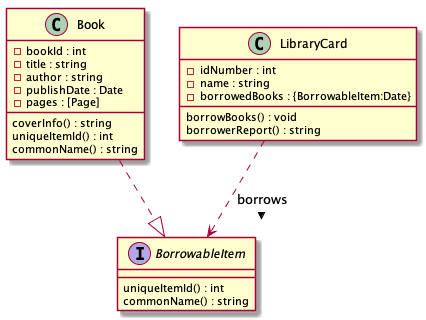
\includegraphics[keepaspectratio]{uml/public interface.png}}
\caption{Class diagram of a book class}
\end{figure}

\subsubsection{Abstraction of
Objects}\label{object-oriented-programming-paradigm.md__abstraction-of-objects}

\begin{quote}
The term abstraction is actually quite overloaded in OOP and CS in
general. The ``abstraction'' I'm talking about in this context is the
concept of abstraction.
\end{quote}

Creating interfaces like these provide OOP with the mechanism to create
\textbf{abstractions} in the object level. An abstraction in computer
science is basically a model of computation that is free from its
implementation. In the same way that functional programming creates
abstractions of mathematical functions by writing lambdas without side
effects, OOP creates abstractions of objects using interfaces that don't
specify the exact implementation of an object.

In the example above, the interface \texttt{BorrowableItem} is an
abstract representation of \emph{something from the library that can be
borrowed}. An interface like \texttt{BorrowableItem} contains method
names and type signatures but it doesn't actually contain code. That is
because a \texttt{BorrowableItem} is an abstract representation. We are
not supposed to care about the implementation of the methods
\texttt{uniqueItemId()} and \texttt{commonName()} all we should care
about is that \texttt{uniqueItemId()} should return an \texttt{int} and
\texttt{commonName()} should return a \texttt{string}.

The reason why this structure still works, is because we have a concrete
class called \texttt{Book} which is a \textbf{realization} or an
\textbf{implementation} of \texttt{BorrowableItem}. A book is
\emph{something from the library that can be borrowed}. Because a
\texttt{Book} is a \texttt{BorrowableItem}, it must also behave based on
the specifications of a \texttt{BorrowableItem}. Meaning it must contain
the methods \texttt{uniqueItemId()} and \texttt{commonName()} (which
should also have the same type signature as the methods of
\texttt{BorrowableItems}). Since \texttt{Book} is a concrete class it's
methods \texttt{uniqueItemId()} and \texttt{commonName()} should be
implemented (meaning there should be code inside these methods).

Why even go through all this trouble? If \emph{something from the
library that can be borrowed} is an abstract idea, what is the point of
modelling it's representation? This looks like extra code just to
represent something that doesn't really have an exact form in the real
world.

For the current structure we created, this feels like extra code because
our system is small enough right now. But imagine if our system grows
and we need to incorporate other things from the library that are not
books but can be borrowed. For example, a library also contains
periodicals that you can borrow as well, and these periodicals do not
follow the form of the book. You need a different representation for a
periodical, therefore you need to create a new concrete class called
\texttt{Periodical}. Since a periodical is also \emph{something from the
library that can be borrowed}, a periodical is another
\textbf{realization} of \texttt{BorrowableItem}. And with the tiny
effort of writing the implementation of a periodical (including the
realized methods \texttt{uniqueItemId()} and \texttt{commonName()} ), we
added an extra interaction that allows a \texttt{LibraryCard} to borrow
periodicals as well.

\begin{figure}
\centering
\pandocbounded{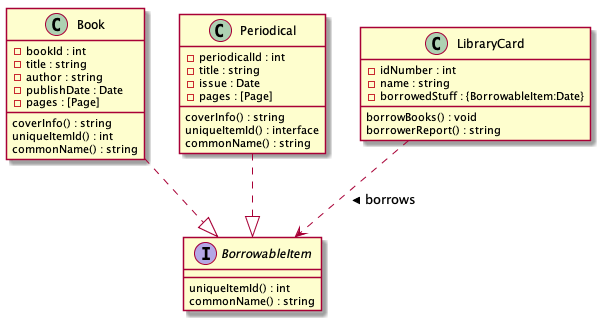
\includegraphics[keepaspectratio]{uml/public interface 2 realizations.png}}
\caption{Class diagram of a book class}
\end{figure}

\subsubsection{The Interface and the
Implementation}\label{object-oriented-programming-paradigm.md__the-interface-and-the-implementation}

Let's summarize what we learned so far by discussing how these
capabilities characterize the philosophy of OOP. The paradigm aims to
solve the issues of state and maintainability by allowing programmers to
create boundaries between its mix of attributes and methods. The
boundaries you enforce are basically the object structure you create. A
library card name shouldn't mix with a book title so we put a boundary
between them by \textbf{encapsulating} them into their respective
objects.

You can imagine these objects as amorphous blobs with surface separating
the methods and attributes inside it from other things in your code.
These amorphous blobs have volume and surface. The volume of these blobs
represent the \textbf{implementation} of these objects and the surface
of these blobs represent the \textbf{interface} of these objects. The
interaction, between two objects is characterized by the surfaces of
objects, the implementation. The volume of the object shouldn't dictate
how the objects relate to each other, in fact everything inside the
object should be inaccessible to other objects. Objects should only see
each other's surface. This means that the interaction between objects
should be defined by their interface not their implementation.

Your job as an OOP programmer is to make sure that the complexity of the
surface grows slower than the complexity of the core. This means that as
your system evolves, changes that happen in the core, the implementation
hidden inside each object, (as much as possible) shouldn't affect the
surface, the interfaces of each object. This is what harmony and
elegance in OOP means. Objects interact with each other seamlessly, and
intuitively, regardless of what their inside look like.

\subsection{Encapsulation}\label{object-oriented-programming-paradigm.md__encapsulation}

One of the most important design principle of object oriented
programming is the concept called encapsulation. I've said it again and
again and I don't mind saying it again right now, oop's innovation that
made the paradigm a solution to the issues of state is its mechanism to
construct boundaries wherever you want (you should want to put it
between irrelevant data). This mechanism is also called
\textbf{encapsulation}. Here are a few important points to remember:

\begin{itemize}
\tightlist
\item
  Encapsulation, when done correctly, makes your system approach a more
  accurate simulation of the real world. The more you encapsulate
  related data and methods, the more you'll create cohesive classes that
  have definite and indivisible purpose.
\item
  You should \textbf{encapsulate what varies}, meaning, things that
  always change should be encapsulated deep into the structure of your
  code. This will help with maintainability since the changing isolated
  data or behavior will have less impact to the to the whole system.
\item
  Encapsulation means both attributes and behaviors. Concrete objects
  should be given the responsibility of implementing their own behavior.
  This means that a method that describes the behavior of a certain
  class should belong to that class.
\end{itemize}

\subsection{Inheritance (you can skip this, there's a better explanation
in Class
Relationships)}\label{object-oriented-programming-paradigm.md__inheritance-you-can-skip-this-theres-a-better-explanation-in-class-relationships}

Another important design principle in OOP is the concept of
\textbf{inheritance}. Inheritance is the concept in which the definition
of a class is derived from another class. An existing class, called the
\textbf{super class} (also called the \textbf{base class} or the
\textbf{parent class}) passes all visible attributes and methods to a
\textbf{sub class} (also called the \textbf{derived class} or the
\textbf{child class}).

The concept of inheritance is also a representation of the real world.
You use inheritance to represent generalizations and specializations. A
super class is a generalization of a sub class and a sub class is a
specialization of a super class.

In this example the supertype animal is a generaliztion of the subtype
mammal. Although it isnt shown, \texttt{Mammal} will also have the
attributes \texttt{name} and \texttt{weight} and the method
\texttt{sound()} since it inherits these from the parent class. Mammal
has a method of its own called \texttt{lactate()} which it doesn share
with animal.

\begin{figure}
\centering
\pandocbounded{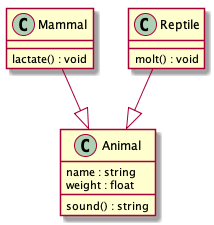
\includegraphics[keepaspectratio]{uml/inheritance.png}}
\caption{inheritance}
\end{figure}

A subclass can also be a super class for another class. This is used to
represent specializations of specializations.

\begin{figure}
\centering
\pandocbounded{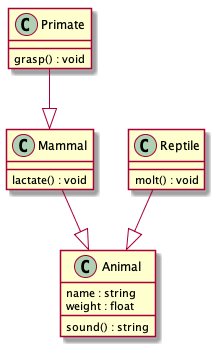
\includegraphics[keepaspectratio]{uml/inheritance2.png}}
\caption{inheritance}
\end{figure}

The class primates will then inherit all visible attributes and mehtods
of \texttt{Mammal} which include those that are inherited from
\texttt{Animal}.

Some programming languages will allow you to add restrictions to the
inheritance of an attribute or a method. Languages like \texttt{C++} or
\texttt{Java} does this using the modifiers \texttt{private} and
\texttt{protected}

\begin{longtable}[]{@{}
  >{\raggedright\arraybackslash}p{(\linewidth - 6\tabcolsep) * \real{0.2857}}
  >{\raggedright\arraybackslash}p{(\linewidth - 6\tabcolsep) * \real{0.2208}}
  >{\raggedright\arraybackslash}p{(\linewidth - 6\tabcolsep) * \real{0.2597}}
  >{\raggedright\arraybackslash}p{(\linewidth - 6\tabcolsep) * \real{0.2338}}@{}}
\toprule\noalign{}
\begin{minipage}[b]{\linewidth}\raggedright
super class visibility
\end{minipage} & \begin{minipage}[b]{\linewidth}\raggedright
public derivation
\end{minipage} & \begin{minipage}[b]{\linewidth}\raggedright
protected derivation
\end{minipage} & \begin{minipage}[b]{\linewidth}\raggedright
private derivation
\end{minipage} \\
\midrule\noalign{}
\endhead
\bottomrule\noalign{}
\endlastfoot
\texttt{public} & \texttt{public} & \texttt{protected} &
\texttt{private} \\
\texttt{protected} & \texttt{protected} & \texttt{protected} &
\texttt{private} \\
\texttt{private} & \emph{not inherited} & \emph{not inherited} &
\emph{not inherited} \\
\end{longtable}

\subsection{Polymorphism}\label{object-oriented-programming-paradigm.md__polymorphism}

Polymorphism literally means \emph{multiple forms}. One of the core
philosophy of OOP allows object instances to exist in multiple forms.
What this means code-wise is that the types of object instances can be
decided during runtime.

\subsubsection{Compile-time
polymorphism}\label{object-oriented-programming-paradigm.md__compile-time-polymorphism}

There's also another type of polymorphism that is not necessarily shared
by all OOP languages, compile-time polymorphism. This is basically the
feature where multiple functions can have the same name as long as they
have different parameter type signatures. This is also known as method
overloading. This concept is also known as dynamic dispatch.

\subsubsection{Run-time
polymorphism}\label{object-oriented-programming-paradigm.md__run-time-polymorphism}

Run-time polymorphism on the other hand, is basically achieved using
specialization and realization relationships between objects. This is
usually what Polymorphism refers to in the scope of OOP.

For example, An object instantiated to be of type \texttt{Primate} is
also an instance of an \texttt{Animal} because a primate is just a
specialization of an animal. This is a reflection of how the real world
works because a primate is indeed an animal. On realization
relationships like a \texttt{Book} and a \texttt{BorrowableItem}, the
same is also true, because a book is also something that can be
borrowed. Realization and specialization relationships guarantee that
you can interact with a sub type as its super type and you can interact
with concrete class as its abstraction.

\section{Optional
Readings}\label{object-oriented-programming-paradigm.md__optional-readings}

Abadi, Martin; Luca Cardelli (1998).
\href{https://link.springer.com/book/10.1007/978-1-4419-8598-9}{A Theory
of Objects. Springer}. ISBN 978-0-387-94775-4.

\chapter{Python
Introduction}\label{python-introduction.md__python-introduction}

\section{starting python from the command
line}\label{python-introduction.md__starting-python-from-the-command-line}

To start python repl on the command line, use the \texttt{python}
command. Make sure you have the path to python saved in your OS's
\texttt{PATH} environment variable. Some python distributions have to be
started with the specific version specified. For these distributions use
the command \texttt{python2} or \texttt{python3}.

\begin{verbatim}
> python
Python 3.8.5 (tags/v3.8.5:580fbb0, Jul 20 2020, 15:43:08) [MSC v.1926 32 bit (Intel)] on win32
Type "help", "copyright", "credits" or "license" for more information.
>>>
\end{verbatim}

To run a python script (\texttt{*.py}), use the same \texttt{python}
command followed by the path to the script

\begin{verbatim}
> python script.py
\end{verbatim}

\section{python syntax}\label{python-introduction.md__python-syntax}

Lets start by discussing simple python syntax. Python code looks like
this

\begin{Shaded}
\begin{Highlighting}[]
\NormalTok{x }\OperatorTok{=} \DecValTok{5}
\NormalTok{value }\OperatorTok{=} \DecValTok{6}
\BuiltInTok{print}\NormalTok{(x }\OperatorTok{+}\NormalTok{ value)}
\end{Highlighting}
\end{Shaded}

The first thing you notice is that python doesn't use semi-colons to
separate statements, python finds the semi-colon redundant since
programmers separate statements using newlines. Here python interprets
three separate statements, \texttt{x\ =\ 5} and \texttt{value\ =\ 6},
and \texttt{print(x\ +\ value)}. The last line is pythons way of
printing to an output stream.

\section{python atomic
types}\label{python-introduction.md__python-atomic-types}

\subsubsection{Integers}\label{python-introduction.md__integers}

An \texttt{int} in python is of course an implementation of an integer
in math. There is no limit to the size of a python integer (except for
system memory).

\begin{Shaded}
\begin{Highlighting}[]
\DecValTok{9999999999999999999999999999} \OperatorTok{+} \DecValTok{1}
\end{Highlighting}
\end{Shaded}

To check the type of a python object, you can use the function
\texttt{type}.

\begin{Shaded}
\begin{Highlighting}[]
\BuiltInTok{type}\NormalTok{(}\DecValTok{9999999999999999999999999999} \OperatorTok{+} \DecValTok{1}\NormalTok{)}
\end{Highlighting}
\end{Shaded}

\begin{Shaded}
\begin{Highlighting}[]
\BuiltInTok{int}
\end{Highlighting}
\end{Shaded}

\subsubsection{Floating-Point
Numbers}\label{python-introduction.md__floating-point-numbers}

A python \texttt{float} is an implementation of a floating point number.
Numbers written in scientific notation are also floating point numbers:

\begin{Shaded}
\begin{Highlighting}[]
\BuiltInTok{type}\NormalTok{(}\FloatTok{4.2}\NormalTok{)}
\end{Highlighting}
\end{Shaded}

\begin{Shaded}
\begin{Highlighting}[]
\BuiltInTok{float}
\end{Highlighting}
\end{Shaded}

\begin{Shaded}
\begin{Highlighting}[]
\BuiltInTok{type}\NormalTok{(}\FloatTok{4.2e5}\NormalTok{)}
\end{Highlighting}
\end{Shaded}

\begin{Shaded}
\begin{Highlighting}[]
\BuiltInTok{float}
\end{Highlighting}
\end{Shaded}

\subsubsection{Complex
numbers}\label{python-introduction.md__complex-numbers}

Complex numbers exist in python. The complex number \(a + bi\) is
represented as \texttt{a\ +\ bj} where \texttt{a} and \texttt{b} are
integer literals.

\begin{Shaded}
\begin{Highlighting}[]
\BuiltInTok{type}\NormalTok{(}\DecValTok{4} \OperatorTok{+} \OtherTok{3j}\NormalTok{)}
\end{Highlighting}
\end{Shaded}

\begin{Shaded}
\begin{Highlighting}[]
\BuiltInTok{complex}
\end{Highlighting}
\end{Shaded}

\subsubsection{Strings}\label{python-introduction.md__strings}

A python \texttt{string} is a sequence of characters. Strings can be
enclosed by single-quotes or double quotes (but you must pair
single-quotes with single-quotes and double-quotes with double quotes).

\begin{Shaded}
\begin{Highlighting}[]
\BuiltInTok{type}\NormalTok{(}\StringTok{\textquotesingle{}This\textquotesingle{}}\NormalTok{)}
\end{Highlighting}
\end{Shaded}

\begin{Shaded}
\begin{Highlighting}[]
\NormalTok{string}
\end{Highlighting}
\end{Shaded}

\begin{Shaded}
\begin{Highlighting}[]
\BuiltInTok{type}\NormalTok{(}\StringTok{"That"}\NormalTok{)}
\end{Highlighting}
\end{Shaded}

\begin{Shaded}
\begin{Highlighting}[]
\NormalTok{string}
\end{Highlighting}
\end{Shaded}

\subsubsection{Boolean}\label{python-introduction.md__boolean}

A \texttt{bool} in python is either \texttt{True} or \texttt{False}.

\begin{Shaded}
\begin{Highlighting}[]
\BuiltInTok{type}\NormalTok{(}\VariableTok{True}\NormalTok{)}
\end{Highlighting}
\end{Shaded}

\begin{Shaded}
\begin{Highlighting}[]
\BuiltInTok{bool}
\end{Highlighting}
\end{Shaded}

\begin{Shaded}
\begin{Highlighting}[]
\BuiltInTok{type}\NormalTok{(}\VariableTok{False}\NormalTok{)}
\end{Highlighting}
\end{Shaded}

\begin{Shaded}
\begin{Highlighting}[]
\BuiltInTok{bool}
\end{Highlighting}
\end{Shaded}

\subsubsection{Python
typing}\label{python-introduction.md__python-typing}

Python is a type inferred, mostly strongly typed, dynamically checked
language.

There are no explicit declarations in python. The first assignment to a
python identifier is its declaration. By assigning a value to that
identifier python infers the type based on the value assigned to it.
Changing the value assigned to an identifier changes its type as well.

\begin{Shaded}
\begin{Highlighting}[]
\NormalTok{x }\OperatorTok{=} \DecValTok{4}
\BuiltInTok{print}\NormalTok{(}\BuiltInTok{type}\NormalTok{(x))}
\NormalTok{x }\OperatorTok{=} \StringTok{\textquotesingle{}this\textquotesingle{}}
\BuiltInTok{print}\NormalTok{(}\BuiltInTok{type}\NormalTok{(x))}
\end{Highlighting}
\end{Shaded}

\begin{Shaded}
\begin{Highlighting}[]
\OperatorTok{\textless{}}\KeywordTok{class} \StringTok{\textquotesingle{}int\textquotesingle{}}\OperatorTok{\textgreater{}}
\OperatorTok{\textless{}}\KeywordTok{class} \StringTok{\textquotesingle{}str\textquotesingle{}}\OperatorTok{\textgreater{}}
\end{Highlighting}
\end{Shaded}

Python is mostly strongly typed, which means that most type conversions
result in a type error.

\begin{quote}
\textbf{Exercise (No submission but try to do this on your own)}

\textbf{Type Coercions}

What do you think would happen if you try to add different types in
python? Without actually executing anything, predict the expected
results of the following type surveys,

\begin{enumerate}
\def\labelenumi{\arabic{enumi}.}
\tightlist
\item
  \texttt{type(3\ +\ 3.0)}
\item
  \texttt{type(3\ +\ \textquotesingle{}3\textquotesingle{})}
\item
  \texttt{type(3\ +\ True)}
\item
  \texttt{type(4/2)}
\item
  \texttt{type(4/0)}
\end{enumerate}

After writing the expected results, write the actual results and compare
them to your expectations.
\end{quote}

Python is dynamically checked, this means that it checks for type safety
during runtime. This means that code that cannot be reached is not type
checked. Which means that the following results in a type error:

\begin{Shaded}
\begin{Highlighting}[]
\BuiltInTok{print}\NormalTok{(}\StringTok{"this"}\OperatorTok{+}\VariableTok{True}\NormalTok{)}
\end{Highlighting}
\end{Shaded}

But the following doesn't:

\begin{Shaded}
\begin{Highlighting}[]
\ControlFlowTok{if} \DecValTok{1} \OperatorTok{==} \DecValTok{0}\NormalTok{:}
    \BuiltInTok{print}\NormalTok{(}\StringTok{"this"}\OperatorTok{+}\VariableTok{True}\NormalTok{)}
\end{Highlighting}
\end{Shaded}

If you choose to do so you can annotate the type of an identifier using
the following syntax:

\begin{Shaded}
\begin{Highlighting}[]
\NormalTok{x:}\BuiltInTok{int} \OperatorTok{=} \DecValTok{3}
\end{Highlighting}
\end{Shaded}

\section{Iterable types}\label{python-introduction.md__iterable-types}

\subsubsection{List}\label{python-introduction.md__list}

A python list, is a vector of any mix of python objects:

\begin{Shaded}
\begin{Highlighting}[]
\BuiltInTok{type}\NormalTok{([}\DecValTok{1}\NormalTok{,}\DecValTok{2}\NormalTok{,}\DecValTok{3}\NormalTok{,}\StringTok{"4"}\NormalTok{,}\VariableTok{True}\NormalTok{,[]])}
\end{Highlighting}
\end{Shaded}

\begin{Shaded}
\begin{Highlighting}[]
\BuiltInTok{list}
\end{Highlighting}
\end{Shaded}

The length of a list can be found using the built-in function
\texttt{len} which accepts an iterable type and returns an integer which
is the length:

\begin{Shaded}
\begin{Highlighting}[]
\BuiltInTok{len}\NormalTok{(l)}
\end{Highlighting}
\end{Shaded}

\begin{Shaded}
\begin{Highlighting}[]
\DecValTok{6}
\end{Highlighting}
\end{Shaded}

Lists can be concatenated using the \texttt{+} operator:

\begin{Shaded}
\begin{Highlighting}[]
\NormalTok{[}\DecValTok{1}\NormalTok{,}\DecValTok{2}\NormalTok{,}\DecValTok{3}\NormalTok{]}\OperatorTok{+}\NormalTok{[}\DecValTok{4}\NormalTok{,}\DecValTok{5}\NormalTok{]}
\end{Highlighting}
\end{Shaded}

\begin{Shaded}
\begin{Highlighting}[]
\NormalTok{[}\DecValTok{1}\NormalTok{, }\DecValTok{2}\NormalTok{, }\DecValTok{3}\NormalTok{, }\DecValTok{4}\NormalTok{, }\DecValTok{5}\NormalTok{]}
\end{Highlighting}
\end{Shaded}

You can check if an element exists in an iterable using the \texttt{in}
operator:

\begin{Shaded}
\begin{Highlighting}[]
\DecValTok{2} \KeywordTok{in}\NormalTok{ [}\DecValTok{1}\NormalTok{,}\DecValTok{2}\NormalTok{,}\DecValTok{3}\NormalTok{,}\StringTok{"4"}\NormalTok{,}\VariableTok{True}\NormalTok{,[]]}
\end{Highlighting}
\end{Shaded}

\begin{Shaded}
\begin{Highlighting}[]
\VariableTok{True}
\end{Highlighting}
\end{Shaded}

List elements are accessed similar to c arrays.

\begin{Shaded}
\begin{Highlighting}[]
\NormalTok{l }\OperatorTok{=}\NormalTok{ [}\DecValTok{1}\NormalTok{,}\DecValTok{2}\NormalTok{,}\DecValTok{3}\NormalTok{,}\StringTok{"4"}\NormalTok{,}\VariableTok{True}\NormalTok{,[]]}
\NormalTok{l[}\DecValTok{2}\NormalTok{]}
\end{Highlighting}
\end{Shaded}

\begin{Shaded}
\begin{Highlighting}[]
\DecValTok{3}
\end{Highlighting}
\end{Shaded}

Negative indices count from the right

\begin{Shaded}
\begin{Highlighting}[]
\NormalTok{l[}\OperatorTok{{-}}\DecValTok{1}\NormalTok{]}
\end{Highlighting}
\end{Shaded}

\begin{Shaded}
\begin{Highlighting}[]
\NormalTok{[]}
\end{Highlighting}
\end{Shaded}

You can extract a copy of a sublist using the following indexing methods

\begin{itemize}
\tightlist
\item
  \texttt{list{[}n:m{]}} produces a sublist from index n to m (including
  the nth element but excluding the mth element).
\item
  \texttt{list{[}:m{]}} equivalent to \texttt{list{[}0:m{]}}.
\end{itemize}

\begin{Shaded}
\begin{Highlighting}[]
\NormalTok{l[}\DecValTok{1}\NormalTok{:}\DecValTok{3}\NormalTok{]}
\end{Highlighting}
\end{Shaded}

\begin{Shaded}
\begin{Highlighting}[]
\NormalTok{[}\DecValTok{2}\NormalTok{,}\DecValTok{3}\NormalTok{]}
\end{Highlighting}
\end{Shaded}

\begin{quote}
\textbf{Exercise (No submission but try to do this on your own) }

\textbf{Advanced list slicing}

Play around with lists and test the behavior of the list access operator
\texttt{::}. What is the result of the expression
\texttt{list{[}a::b{]}} where \texttt{list} is a \texttt{list} and
\texttt{a} and \texttt{b} are \texttt{int}s? What about
\texttt{list{[}a::{]}} and \texttt{list{[}::b{]}}.
\end{quote}

A python list is mutable, you can change the value of a specific element
or range:

\begin{Shaded}
\begin{Highlighting}[]
\NormalTok{l[}\DecValTok{1}\NormalTok{] }\OperatorTok{=} \DecValTok{0}
\NormalTok{l}
\end{Highlighting}
\end{Shaded}

\begin{Shaded}
\begin{Highlighting}[]
\NormalTok{[}\DecValTok{1}\NormalTok{, }\DecValTok{0}\NormalTok{, }\DecValTok{3}\NormalTok{, }\StringTok{\textquotesingle{}4\textquotesingle{}}\NormalTok{, }\VariableTok{True}\NormalTok{, []]}
\end{Highlighting}
\end{Shaded}

You can delete an element on a specific index or range:

\begin{Shaded}
\begin{Highlighting}[]
\KeywordTok{del}\NormalTok{ l[}\DecValTok{2}\NormalTok{]}
\NormalTok{l}
\end{Highlighting}
\end{Shaded}

\begin{Shaded}
\begin{Highlighting}[]
\NormalTok{[}\DecValTok{1}\NormalTok{, }\DecValTok{0}\NormalTok{, }\StringTok{\textquotesingle{}4\textquotesingle{}}\NormalTok{, }\VariableTok{True}\NormalTok{, []]}
\end{Highlighting}
\end{Shaded}

\begin{Shaded}
\begin{Highlighting}[]
\KeywordTok{del}\NormalTok{ l[}\DecValTok{2}\NormalTok{:}\DecValTok{4}\NormalTok{]}
\NormalTok{l}
\end{Highlighting}
\end{Shaded}

\begin{Shaded}
\begin{Highlighting}[]
\NormalTok{[}\DecValTok{1}\NormalTok{, }\DecValTok{0}\NormalTok{, []]}
\end{Highlighting}
\end{Shaded}

\subsubsection{Tuples}\label{python-introduction.md__tuples}

A python \texttt{tuple} is an immutable collection of objects. Tuples
are written surrounded by parentheses instead of square brackets.

\begin{Shaded}
\begin{Highlighting}[]
\NormalTok{t }\OperatorTok{=}\NormalTok{ (}\DecValTok{1}\NormalTok{,}\DecValTok{2}\NormalTok{,}\VariableTok{True}\NormalTok{,}\DecValTok{5}\NormalTok{,}\DecValTok{6}\NormalTok{)}
\end{Highlighting}
\end{Shaded}

Tuple elements and subtuples can be accessed the same way with lists.

\begin{Shaded}
\begin{Highlighting}[]
\NormalTok{t[}\DecValTok{2}\NormalTok{]}
\end{Highlighting}
\end{Shaded}

\begin{Shaded}
\begin{Highlighting}[]
\VariableTok{True}
\end{Highlighting}
\end{Shaded}

\begin{Shaded}
\begin{Highlighting}[]
\NormalTok{t[}\DecValTok{1}\NormalTok{:}\DecValTok{4}\NormalTok{]}
\end{Highlighting}
\end{Shaded}

\begin{Shaded}
\begin{Highlighting}[]
\NormalTok{(}\DecValTok{2}\NormalTok{, }\VariableTok{True}\NormalTok{, }\DecValTok{5}\NormalTok{)}
\end{Highlighting}
\end{Shaded}

Tuples can also be concatenated similar to lists.

\begin{Shaded}
\begin{Highlighting}[]
\NormalTok{(}\DecValTok{1}\NormalTok{,}\DecValTok{2}\NormalTok{,}\DecValTok{3}\NormalTok{) }\OperatorTok{+}\NormalTok{ (}\DecValTok{5}\NormalTok{,}\DecValTok{6}\NormalTok{)}
\end{Highlighting}
\end{Shaded}

\begin{Shaded}
\begin{Highlighting}[]
\NormalTok{(}\DecValTok{1}\NormalTok{, }\DecValTok{2}\NormalTok{, }\DecValTok{3}\NormalTok{, }\DecValTok{5}\NormalTok{, }\DecValTok{6}\NormalTok{)}
\end{Highlighting}
\end{Shaded}

Tuples are immutable so you cannot change the elements of a tuple.

\begin{Shaded}
\begin{Highlighting}[]
\NormalTok{t[}\DecValTok{1}\NormalTok{] }\OperatorTok{=} \DecValTok{2}
\end{Highlighting}
\end{Shaded}

\begin{Shaded}
\begin{Highlighting}[]
\NormalTok{...}
\PreprocessorTok{TypeError}\NormalTok{: }\StringTok{\textquotesingle{}tuple\textquotesingle{}} \BuiltInTok{object}\NormalTok{ does }\KeywordTok{not}\NormalTok{ support item assignment}
\end{Highlighting}
\end{Shaded}

\subsubsection{Dictionaries}\label{python-introduction.md__dictionaries}

A python dictionary is a collection of key-value pairs. It is written
surrounded by curly braces. Each pair is written,
\texttt{\textless{}key\textgreater{}:\textless{}value\textgreater{}}

\begin{Shaded}
\begin{Highlighting}[]
\NormalTok{d }\OperatorTok{=}\NormalTok{ \{}\StringTok{"a"}\NormalTok{:}\DecValTok{1}\NormalTok{,}\DecValTok{0}\NormalTok{:}\StringTok{"this"}\NormalTok{,}\StringTok{"b"}\NormalTok{:}\VariableTok{True}\NormalTok{\}}
\end{Highlighting}
\end{Shaded}

The elements of a dictionary can be accessed using the keys. Here the
value associated to the key ``a'' is accessed.

\begin{Shaded}
\begin{Highlighting}[]
\NormalTok{d[}\StringTok{"a"}\NormalTok{]}
\end{Highlighting}
\end{Shaded}

\begin{Shaded}
\begin{Highlighting}[]
\DecValTok{1}
\end{Highlighting}
\end{Shaded}

Here the value associated to the key \texttt{0} is accessed.

\begin{Shaded}
\begin{Highlighting}[]
\NormalTok{d[}\DecValTok{0}\NormalTok{]}
\end{Highlighting}
\end{Shaded}

\begin{Shaded}
\begin{Highlighting}[]
\CommentTok{"this"}
\end{Highlighting}
\end{Shaded}

To check if a specific key exists in the dictionary, use the \texttt{in}
operator in the same way you use it in lists:

\begin{Shaded}
\begin{Highlighting}[]
\CommentTok{"b"} \KeywordTok{in}\NormalTok{ d}
\end{Highlighting}
\end{Shaded}

\begin{verbatim}
True
\end{verbatim}

You can add new entries to the dictionary using the following syntax:
Notice how the dictionary has new entries after the second line

\begin{Shaded}
\begin{Highlighting}[]
\BuiltInTok{print}\NormalTok{(d)}
\NormalTok{d[}\StringTok{"newKey"}\NormalTok{]}\OperatorTok{=}\StringTok{"newValue"}
\BuiltInTok{print}\NormalTok{(d)}
\end{Highlighting}
\end{Shaded}

\begin{verbatim}
{'a': 1, 0: 'this', 'b': True}
{'a': 1, 0: 'this', 'b': True, 'newKey': 'newValue'}
\end{verbatim}

Key-value associations are injective meaning, a key can only be
associated to exactly one value. If you attempt to ``add'' an entry for
a key that already exists, it will not create a new entry, it will
instead overwrite the old value:

\begin{Shaded}
\begin{Highlighting}[]
\BuiltInTok{print}\NormalTok{(d)}
\NormalTok{d[}\StringTok{"newKey"}\NormalTok{]}\OperatorTok{=}\StringTok{"newerValue"}
\BuiltInTok{print}\NormalTok{(d)}
\end{Highlighting}
\end{Shaded}

\begin{verbatim}
{'a': 1, 0: 'this', 'b': True, 'newKey': 'newValue'}
{'a': 1, 0: 'this', 'b': True, 'newKey': 'newerValue'}
\end{verbatim}

To remove entries in the dictionary use \texttt{del} in the same way you
use it on lists:

\begin{Shaded}
\begin{Highlighting}[]
\KeywordTok{del}\NormalTok{ d[}\StringTok{"a"}\NormalTok{]}
\BuiltInTok{print}\NormalTok{(d)}
\end{Highlighting}
\end{Shaded}

\begin{verbatim}
{0: 'this', 'b': True, 'newKey': 'newerValue'}
\end{verbatim}

\section{Selection
expressions}\label{python-introduction.md__selection-expressions}

Python's if else statements follow this pattern (the else part can be
omitted if the execution does not need an alternative). The colon and
whitespace are part of the syntax and are mandatory. Every tabulated
line is inside the scope of the \texttt{if} part or the \texttt{else}
part.

\begin{Shaded}
\begin{Highlighting}[]
\ControlFlowTok{if}\NormalTok{ boolean:}
\NormalTok{    truePart}
\ControlFlowTok{else}\NormalTok{:}
\NormalTok{    alternativePart}
\end{Highlighting}
\end{Shaded}

Nesting if else statements in python has a shortcut. The following code:

\begin{Shaded}
\begin{Highlighting}[]
\ControlFlowTok{if} \VariableTok{False}\NormalTok{:}
    \BuiltInTok{print}\NormalTok{(}\StringTok{"won\textquotesingle{}t print"}\NormalTok{)}
\ControlFlowTok{else}\NormalTok{:}
    \ControlFlowTok{if} \VariableTok{False}\NormalTok{:}
        \BuiltInTok{print}\NormalTok{(}\StringTok{"won\textquotesingle{}t print too"}\NormalTok{)}
    \ControlFlowTok{else}\NormalTok{:}
        \BuiltInTok{print}\NormalTok{(}\StringTok{"will print"}\NormalTok{)}
\end{Highlighting}
\end{Shaded}

Can be summarized to this:

\begin{Shaded}
\begin{Highlighting}[]
\ControlFlowTok{if} \VariableTok{False}\NormalTok{:}
    \BuiltInTok{print}\NormalTok{(}\StringTok{"won\textquotesingle{}t print"}\NormalTok{)}
\ControlFlowTok{elif} \VariableTok{False}\NormalTok{:}
    \BuiltInTok{print}\NormalTok{(}\StringTok{"won\textquotesingle{}t print too"}\NormalTok{)}
\ControlFlowTok{else}\NormalTok{:}
    \BuiltInTok{print}\NormalTok{(}\StringTok{"will print"}\NormalTok{)}
\end{Highlighting}
\end{Shaded}

Python also understands ternary expressions:

\begin{Shaded}
\begin{Highlighting}[]
\NormalTok{x }\OperatorTok{=} \StringTok{"this"} \ControlFlowTok{if} \VariableTok{True} \ControlFlowTok{else} \StringTok{"That"}
\BuiltInTok{print}\NormalTok{(x)}
\end{Highlighting}
\end{Shaded}

\begin{Shaded}
\begin{Highlighting}[]
\NormalTok{this}
\end{Highlighting}
\end{Shaded}

The value of \texttt{x} will depend on the value of the condition. Since
this is true, the whole ternary expression reduces to \texttt{"this"}

\section{Iteration}\label{python-introduction.md__iteration}

Python's \texttt{while} loop is similar to C's while loop. The block of
code inside the while loop will be executed repeatedly until the
condition becomes false.

\begin{Shaded}
\begin{Highlighting}[]
\NormalTok{i }\OperatorTok{=} \DecValTok{0}
\ControlFlowTok{while}\NormalTok{ i }\OperatorTok{\textless{}} \DecValTok{5}\NormalTok{:}
    \BuiltInTok{print}\NormalTok{(i)}
\NormalTok{    i}\OperatorTok{+=}\DecValTok{1}
\end{Highlighting}
\end{Shaded}

\begin{Shaded}
\begin{Highlighting}[]
\DecValTok{0}
\DecValTok{1}
\DecValTok{2}
\DecValTok{3}
\DecValTok{4}
\end{Highlighting}
\end{Shaded}

Python's \texttt{for} loop is different from C. Python's \texttt{for}
loop is a collections loop similar to Java's \texttt{foreach}
expression.

\begin{Shaded}
\begin{Highlighting}[]
\ControlFlowTok{for}\NormalTok{ i }\KeywordTok{in}\NormalTok{ [}\StringTok{"this"}\NormalTok{,}\DecValTok{2}\NormalTok{,}\VariableTok{True}\NormalTok{,}\DecValTok{4}\NormalTok{]:}
    \BuiltInTok{print}\NormalTok{(i)}
\end{Highlighting}
\end{Shaded}

\begin{verbatim}
this
2
True
4
\end{verbatim}

This for loop can be interpreted in common language as, \emph{For every
element \(i\) in {[}``this'',2,True,4{]}, print \(i\)}. Inside the for
loop, the value of \texttt{i} refers to the elements inside the list. At
the first execution of \texttt{print(i)}, \texttt{i} refers to the first
element of the list. At the second execution \texttt{i} refers to the
2nd element of the list. and so on until it exhausts the list.

A common pattern for a \texttt{for} loop is something like this:

\begin{Shaded}
\begin{Highlighting}[]
\ControlFlowTok{for}\NormalTok{ i }\KeywordTok{in} \BuiltInTok{range}\NormalTok{(}\DecValTok{0}\NormalTok{,}\DecValTok{5}\NormalTok{):}
    \BuiltInTok{print}\NormalTok{(i)}
\end{Highlighting}
\end{Shaded}

\begin{Shaded}
\begin{Highlighting}[]
\DecValTok{0}
\DecValTok{1}
\DecValTok{2}
\DecValTok{3}
\DecValTok{4}
\end{Highlighting}
\end{Shaded}

The function \texttt{range} produces a list of integers, starting from
\texttt{0} until the \texttt{4}. \texttt{range(0,5)} can even be
shortened to \texttt{range(5)}.

\section{Python
functions}\label{python-introduction.md__python-functions}

Python functions are written using the following syntax:

\begin{Shaded}
\begin{Highlighting}[]
\KeywordTok{def}\NormalTok{ f(parameters):}
\NormalTok{    body}
\end{Highlighting}
\end{Shaded}

For example creating the add function:

\begin{Shaded}
\begin{Highlighting}[]
\KeywordTok{def}\NormalTok{ add(x,y):}
    \ControlFlowTok{return}\NormalTok{ x }\OperatorTok{+}\NormalTok{ y}
\end{Highlighting}
\end{Shaded}

\section{Python file reading and
writing}\label{python-introduction.md__python-file-reading-and-writing}

\subsection{Opening a
file}\label{python-introduction.md__opening-a-file}

To open file in python

\begin{Shaded}
\begin{Highlighting}[]
\NormalTok{f }\OperatorTok{=} \BuiltInTok{open}\NormalTok{(}\StringTok{"input.in"}\NormalTok{,}\StringTok{"a"}\NormalTok{) }
\end{Highlighting}
\end{Shaded}

The first parameter is the path to the file and the second parameter is
the mode the file opening

\begin{itemize}
\tightlist
\item
  \texttt{"a"} - append mode
\item
  \texttt{"a+"} - append mode but if the file being opened does not
  exist, create the file and append
\item
  \texttt{"w"} - for write mode (overwrites the contents of the file)
\item
  \texttt{"w+"} - write mode but if the file being opened does not
  exist, create the file and write
\item
  \texttt{"r"} - read mode
\item
  \texttt{"r+"} - read mode but if the file being opened does not exist,
  create the file and read
\end{itemize}

\subsection{Writing to a
file}\label{python-introduction.md__writing-to-a-file}

To write a single line in the file use the method \texttt{write()}. If
the file is opened using \texttt{"a"} and \texttt{"a+"} mode the string
is appended to the file. If it is opened using \texttt{w} and
\texttt{w+} modes, the files contents are overwritten by this new line.
Will not work on \texttt{"r"} and \texttt{"r"+} modes.

\begin{Shaded}
\begin{Highlighting}[]
\NormalTok{f.write(}\StringTok{"foo"}\NormalTok{)}
\end{Highlighting}
\end{Shaded}

\subsection{Reading from a
file}\label{python-introduction.md__reading-from-a-file}

To read an entire file use the method \texttt{read()}. This function
returns the whole file as a string

\begin{Shaded}
\begin{Highlighting}[]
\NormalTok{f.read()}
\end{Highlighting}
\end{Shaded}

\subsection{Closing a
file}\label{python-introduction.md__closing-a-file}

\begin{Shaded}
\begin{Highlighting}[]
\NormalTok{f.close()}
\end{Highlighting}
\end{Shaded}

\section{Formatted
Strings}\label{python-introduction.md__formatted-strings}

When working with multiple string concatenations you can use formatted
strings. For example, the following string

\begin{Shaded}
\begin{Highlighting}[]
\NormalTok{s }\OperatorTok{=} \StringTok{"this"}
\NormalTok{t }\OperatorTok{=} \StringTok{"is"}
\NormalTok{u }\OperatorTok{=} \StringTok{"tedious"}
\NormalTok{v }\OperatorTok{=} \StringTok{"times"}
\NormalTok{w }\OperatorTok{=} \DecValTok{100}

\NormalTok{c }\OperatorTok{=}\NormalTok{ s }\OperatorTok{+} \StringTok{" "} \OperatorTok{+}\NormalTok{ t }\OperatorTok{+} \StringTok{" "} \OperatorTok{+}\NormalTok{ u }\OperatorTok{+} \StringTok{" "} \OperatorTok{+}\NormalTok{ v }\OperatorTok{+} \StringTok{" "} \OperatorTok{+} \BuiltInTok{str}\NormalTok{(w)}
\BuiltInTok{print}\NormalTok{(c)}
\end{Highlighting}
\end{Shaded}

\begin{verbatim}
this is tedious times 100
\end{verbatim}

Can be concatenated similar to C's formatting using the \texttt{\%}
operator

\begin{Shaded}
\begin{Highlighting}[]
\NormalTok{s }\OperatorTok{=} \StringTok{"this"}
\NormalTok{t }\OperatorTok{=} \StringTok{"is"}
\NormalTok{u }\OperatorTok{=} \StringTok{"tedious"}
\NormalTok{v }\OperatorTok{=} \StringTok{"times"}
\NormalTok{w }\OperatorTok{=} \DecValTok{100}

\NormalTok{c }\OperatorTok{=} \StringTok{"}\SpecialCharTok{\%s}\StringTok{ }\SpecialCharTok{\%s}\StringTok{ }\SpecialCharTok{\%s}\StringTok{ }\SpecialCharTok{\%s}\StringTok{ }\SpecialCharTok{\%d}\StringTok{"} \OperatorTok{\%}\NormalTok{ (s,t,u,v,w)}
\BuiltInTok{print}\NormalTok{(c)}
\end{Highlighting}
\end{Shaded}

\begin{verbatim}
this is tedious times 100
\end{verbatim}

\section{Type
Annotations}\label{python-introduction.md__type-annotations}

Type annotations mark the type of identifiers.

\begin{Shaded}
\begin{Highlighting}[]
\NormalTok{x:}\BuiltInTok{int} \OperatorTok{=} \DecValTok{1}
\NormalTok{s:}\BuiltInTok{str} \OperatorTok{=} \StringTok{"Hey"}
\end{Highlighting}
\end{Shaded}

You can also annotations to set the parameter types and the return type
of a function

\begin{Shaded}
\begin{Highlighting}[]
\KeywordTok{def}\NormalTok{ add(x:}\BuiltInTok{int}\NormalTok{,y:}\BuiltInTok{int}\NormalTok{) }\OperatorTok{{-}\textgreater{}} \BuiltInTok{int}\NormalTok{:}
    \ControlFlowTok{return}\NormalTok{ x }\OperatorTok{*}\NormalTok{ y}
\end{Highlighting}
\end{Shaded}

Type annotations are only annotations, you don't have to write them. But
writing them will help you make sense of a complicated system

\section{Python library
import}\label{python-introduction.md__python-library-import}

To import python libraries use the keyword \texttt{import} followed by
the python library name. As much as possible write imports at the
topmost part of your python files

\begin{Shaded}
\begin{Highlighting}[]
\ImportTok{import}\NormalTok{ math}
\NormalTok{math.ceil(}\FloatTok{1.5}\NormalTok{)}
\end{Highlighting}
\end{Shaded}

\begin{verbatim}
2
\end{verbatim}

You can give the library name a shorter alias for convenience

\begin{Shaded}
\begin{Highlighting}[]
\ImportTok{import}\NormalTok{ math }\ImportTok{as}\NormalTok{ m}
\NormalTok{m.ceil(}\FloatTok{1.5}\NormalTok{)}
\end{Highlighting}
\end{Shaded}

\begin{verbatim}
2
\end{verbatim}

You can also choose not to import the whole library, just specific
classes and functions. When you do this you can directly access the
class or function without the dot reference.

\begin{Shaded}
\begin{Highlighting}[]
\ImportTok{from}\NormalTok{ math }\ImportTok{import}\NormalTok{ floor,ceil }\CommentTok{\#importing floor,and ceil only}
\NormalTok{floor(}\FloatTok{1.2}\NormalTok{) }\OperatorTok{+}\NormalTok{ ceil(}\FloatTok{1.5}\NormalTok{)}
\end{Highlighting}
\end{Shaded}

\begin{verbatim}
3
\end{verbatim}

If you are importing your own files, the same syntax will work as long
as you are in the same directory as the python file you are importing.

\begin{Shaded}
\begin{Highlighting}[]
\ImportTok{from}\NormalTok{ myPythonFile }\ImportTok{import}\NormalTok{ someMethod, someFile}
\end{Highlighting}
\end{Shaded}

\begin{quote}
Assuming \texttt{myPythonFile.py} exists in the same directory you are
currently in
\end{quote}

\section{Python comments}\label{python-introduction.md__python-comments}

Comments are made using the octothorpe/pound/hash/sharp symbol
(\texttt{\#})

\begin{Shaded}
\begin{Highlighting}[]
\DecValTok{1} \OperatorTok{+} \DecValTok{1} \CommentTok{\#comments are made using the octothorpe/pound/hash/sharp symbol}
\end{Highlighting}
\end{Shaded}

\chapter{Class
Relationships}\label{class-relationships.md__class-relationships}

\section{Introduction}\label{class-relationships.md__introduction}

The interactions between one an instance of a class to another is
largely characterized by the relationship between them. Here we talk
about relationships that define the polymorphism between classes and
relationships that define dependency between objects.

\section{Learning
Outcomes}\label{class-relationships.md__learning-outcomes}

\begin{enumerate}
\def\labelenumi{\arabic{enumi}.}
\tightlist
\item
  Differentiate realization relationships and specialization
  relationships
\item
  Describe how class abstract methods work in realization relationships
\item
  Describe the concept of inheritance
\item
  Differentiate aggregation relationships and composition relationships
\end{enumerate}

\begin{center}\rule{0.5\linewidth}{0.5pt}\end{center}

\section{Type Based
Relationships}\label{class-relationships.md__type-based-relationships}

Type based relationships are characterized by how two classes are
related to each other through ontological hierarchy. A mammal class's
relationship with an animal class's relationship is type based. That is
because a mammal is considered as an animal while an animal is not
necessarily a mammal.

There are two type based relationships (there can be an extra one which
is a type relationship that is sort of a hybrid of the two).

\subsection{Realization}\label{class-relationships.md__realization}

A realization relationship is a one way relationship that describes how
something abstract is REALized by something concrete. Given a
\texttt{Realization} class and an \texttt{Abstraction} class, The
\texttt{Realization} class realizes the \texttt{Abstraction} class.

\begin{quote}
A realization relationship is also called an \textbf{implementation}
relationship. An implementation, implements some interface.
\textbf{Interface} is also a fitting term for abstractions because it is
through these classes that other objects interact with each other.
\end{quote}

An \texttt{Abstraction} is a special type of class that does not contain
any implementation. This means that \texttt{Abstraction} doesn't have
code that controls the form and behavior of the class. It only contains
code that specify how this class interacts with other objects. This
means that abstract classes only contain method names and type
signatures with empty bodies.

These \texttt{Abstraction} classes appear useless at first since it
doesn't do anything at all. In fact you cannot even create an instance
of an abstraction. Even if you do it will be pointless since it doesn't
have code that controls how it behaves.

An abstraction can only be useful if some other class realizes this
abstraction. These \texttt{Realization} classes provide abstractions
their form and behavior.

\textbf{What's the point in maintaining some realization relationship
between classes? If abstractions can only be used through their
realizations , then why create the abstraction at all?}

The importance of this seemingly pointless relationship lies in OOP's
data hiding principle. We will explore more about why these
relationships are very common in a future discussion about SOLID
principles. For now I'll show one of the reasons why this is useful
through an example:

\begin{figure}
\centering
\pandocbounded{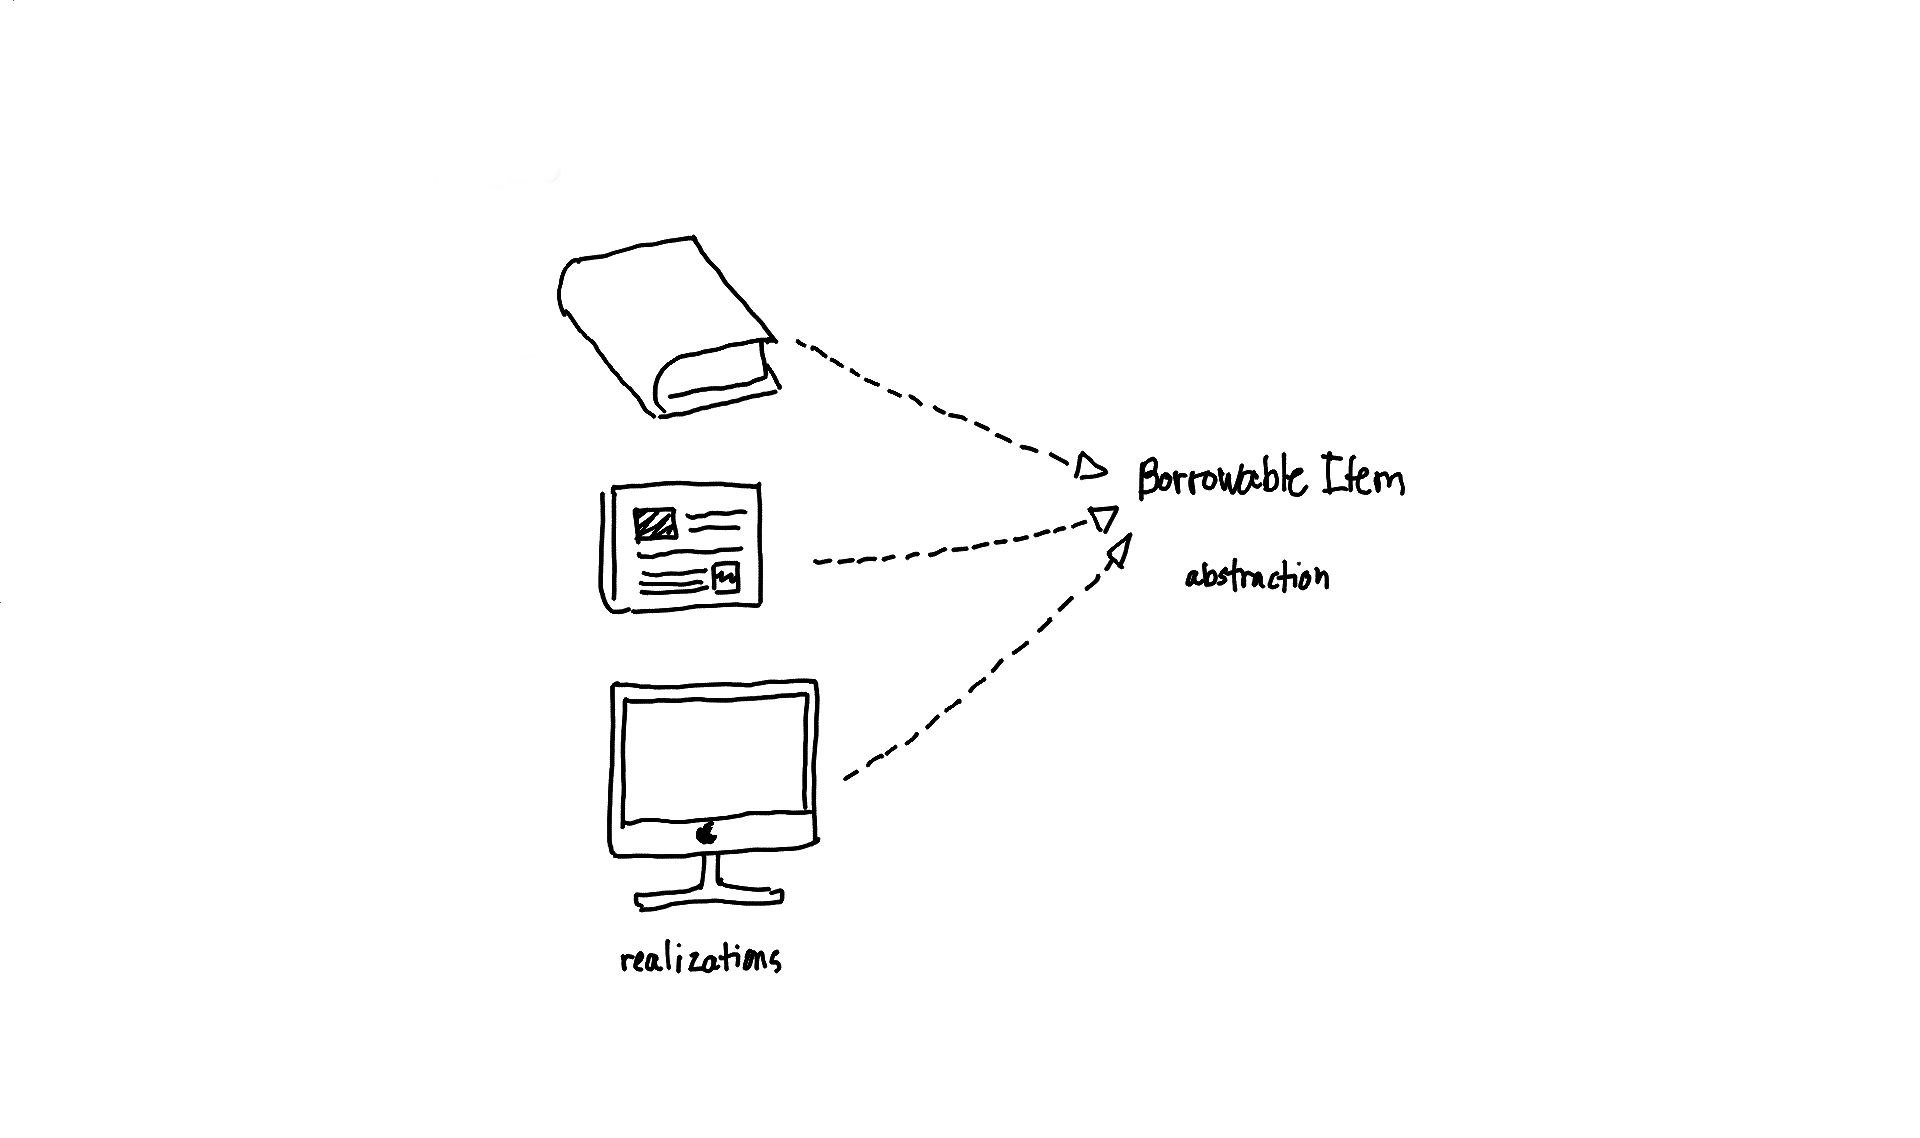
\includegraphics[keepaspectratio]{https://raw.githubusercontent.com/HowDoIGitHelp/CMSC23MDNotes/master/Markdown\%20Lecture\%20Notes\%20and\%20Lab\%20Exercises/copyright\%20free\%20drawings/RealizationRelationship.png}}
\caption{Realization Relationship Example}
\end{figure}

Consider a library system. In a library, you are able to borrow
resources such as books, newspapers, and computers. When the library
system interacts with these resources to facilitate transactions such as
borrowing and returning, the library system treats these resource like
general \textbf{Borrowable Items}. It doesn't really need to concern
itself of the specific type. Operating like this is better for the
library system for reasons such as maintainability and future proofing
(this will be explained in detail in when we discuss SOLID design
principles). Therefore, the best architecture to use in this situation
is to make each resource type a realization of Borrowable Item. A
\texttt{BorrowableItem} class would merely be an abstraction. This class
would contain no behavior or form, it only contains specifications of
how to interact with it. And it does make sense, I mean, how exactly
does a general borrowable item behave or look like? It's abstract. What
we know is that any \texttt{BorrowableItem} can be borrowed or returned
so we write empty \texttt{borrow()} and \texttt{return()} functions (it
specifies how it interacts with others but it doesn't have any specific
behavior, these methods are called abstract methods).

Any realization of \texttt{BorrowableItem}, such as \texttt{Book} or
\texttt{Newspaper} will be forced to implement the \texttt{borrow()} and
\texttt{return()} methods as well (btw all realizations are forced to
implement the methods of its abstraction), meaning it needs to include
these methods with each of their own method bodies for borrowing and
returning (if books and newspapers are borrowed or returned in different
manners, then you write different method bodies for each).

\begin{quote}
Realizations can also have extra methods that are not present in the
abstractions.
\end{quote}

This is how realization relationships enable \textbf{polymorphism}, a
\texttt{Book} is a \texttt{BorrowableItem}, allowing the library system
to interact with it like any \texttt{BorrowableItem}. But at the same
time \texttt{Book} is a book so it behaves in the manner a book behaves.

By building all of these relationships, the library system is able
interact with resources without explicitly knowing which exact resource
it is. The system knows that it is borrowing some instance of a
borrowable item but it does not know if it is a book or a newspaper. The
exact type of this instance will then behave depending on its type.
Although all this effort may seem unnecessary, you will learn in this
course that through the establishment of these relationships, OOP is
able to uphold one of its core design principles, \textbf{data-hiding}.

Abstractions can also realize abstractions. For example given an
abstraction A, another abstraction, called B, can realize A. A class C
then realizes B. When this happens, B does not need to implement A's
abstract methods because B is an abstraction itself. Therefore, C will
inherit all of A and B's abstract methods. The abstract methods of an
abstraction cascades down to the realization realizing any of its
realizations as well.

In this case C instances can be treated as B instances or A instances
but it will behave in the way C behaves.

\subsection{Specialization}\label{class-relationships.md__specialization}

Specialization relationships are very similar to realization
relationships. You can think of these specialization relationships as
realizations but between two real/concrete classes. A specialized class
specializes some general class. By establishing this relationship, you
are able to extend the form and behavior of a specific class.

\begin{quote}
Specialization has plenty of names. This relationship is also called
\textbf{extension} between the special/child/sub class and
general/parent/super class. Another name for it would be
\textbf{inheritance}.
\end{quote}

\begin{figure}
\centering
\pandocbounded{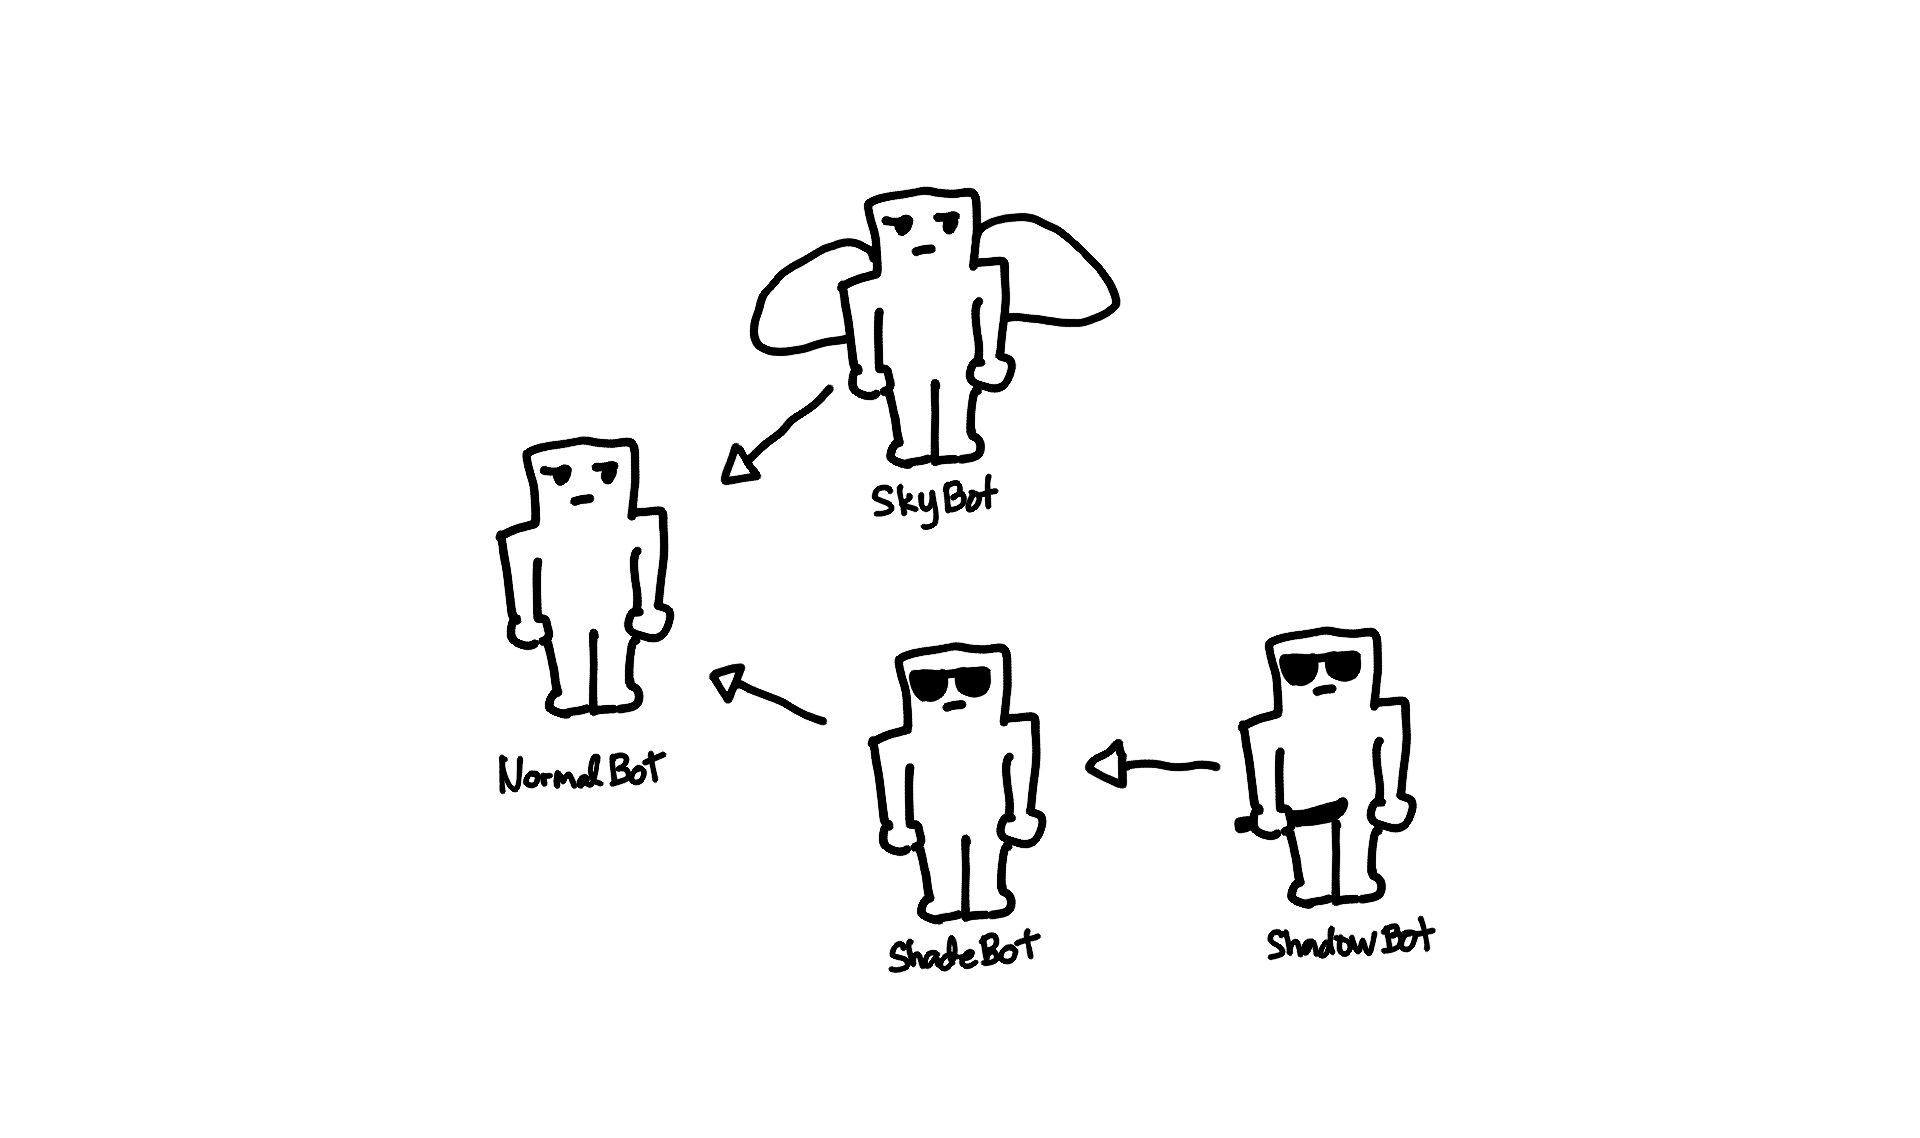
\includegraphics[keepaspectratio]{https://raw.githubusercontent.com/HowDoIGitHelp/CMSC23MDNotes/master/Markdown\%20Lecture\%20Notes\%20and\%20Lab\%20Exercises/copyright\%20free\%20drawings/SpecializationRelationship.png}}
\caption{Specialization Example}
\end{figure}

Here's an example that would illustrate what the specialization
relationship means. Consider a factory that builds robots. This factory
is able to build \texttt{NormalBot}s which are the general type of
robots. Instead of creating entirely separate mechanisms to build each
type of robot, the factory is able to exploit the fact that other robots
are just specializations of \texttt{NormalBot}. \texttt{Skybot} is just
the same as \texttt{NormalBot} but it has extra flight capabilities.
\texttt{ShadeBot} is just the same as \texttt{NormalBot} but it has UV
Protection. Because of this the factory is able to use the building
recipes for \texttt{NormalBot} to build \texttt{Skybot} and
\texttt{ShadeBot}. All they need to do is to add some extra layers of
construction such as adding wings or outfitting shades.

Specialization relationships work like this as well. When you write code
for the general class, you do not need to rewrite it for
specializations. What you write inside specializations are the the
attributes and method that make it special. If this specialization has
flight capabilities then add attributes for wings and methods for
flight. If this specialization behave in a different manner for some
specific method then you only change that specific method.

Because of this relationship, you only need to write one copy of the
code that is common for the general class and its specializations. This
means that you do not need to rewrite said code, saving time and effort
but more importantly, having one copy of code helps for maintainability.
When the recipe of all robot types need to change, the factory only
needs to change the recipe of \texttt{NormalBot}, all of the special
robots' recipes will change as well since they all use
\texttt{NormalBot}'s recipe. When the code for the general class and the
special classes need to be updated, changing the shared code found
inside the general class will automatically affect special classes.
Through this mechanism, specialization relationships enable
\textbf{inheritance}, one of OOP's core design principle.

\begin{quote}
This is where the terms \textbf{inheritance} and extension make sense.
Special class inherit all of the attributes and methods of the general
class. Special classes can also be thought of as extensions of the
general class, since these special classes extend or tweak the
capabilities of the general class.
\end{quote}

You can also specialize, specializations. This is illustrated by
\texttt{ShadowBot}, which is a special \texttt{ShadeBot} that has knife.
Since \texttt{ShadowBot} is a special \texttt{ShadeBot} and
\texttt{ShadeBot} is a special \texttt{NormalBot}, \texttt{ShadowBot} is
automatically a specialization of \texttt{NormalBot} as well.

Specializations also allow polymorphism in the same way realizations do.
A \texttt{ShadowBot} can be interacted with like any \texttt{NormalBot}
or \texttt{ShadeBot} but since it is also a \texttt{ShadowBot} it will
behave specifically like a \texttt{ShadowBot}.

\subsection{Abstract
Classes}\label{class-relationships.md__abstract-classes}

An abstract class is something in between an abstraction and a
generalization. It contains attributes and methods with bodies but it
also contains abstract methods as well. When classes specialize/realize
abstract classes, they inherit the attributes and methods with bodies
but they are forced to implement the abstract methods as well. These
relationships are sometimes used if the system requires a mix of
inheritance and implementation between classes.

\subsection{Multiple Type
Relationships}\label{class-relationships.md__multiple-type-relationships}

It is possible for a class to realize/specialize multiple
abstractions/generalizations. For example, given abstractions, A,B and
C, and generalizations E,F, and G, a class X can realize/specialize all
of them. When you do this, X will be forced to inherit all of the
abstract methods in A, B and C, and automatically inherit everything
from E, F, and G.

\section{Dependency
Relationships}\label{class-relationships.md__dependency-relationships}

Dependency relationships, also known as \textbf{associations},
characterize how two classes interact with each other. A class which is
dependent on another class, needs to know how to interact with it. These
interactions range from being used as method parameters, being returned
in methods, being used inside method bodies, being used as attributes
and etc. A dependency relationship is one way (but it is also possible
for two objects to be dependent on each other). A \textbf{client} class
is dependent on some \textbf{dependency}. There are two types of
dependencies:

\begin{figure}
\centering
\pandocbounded{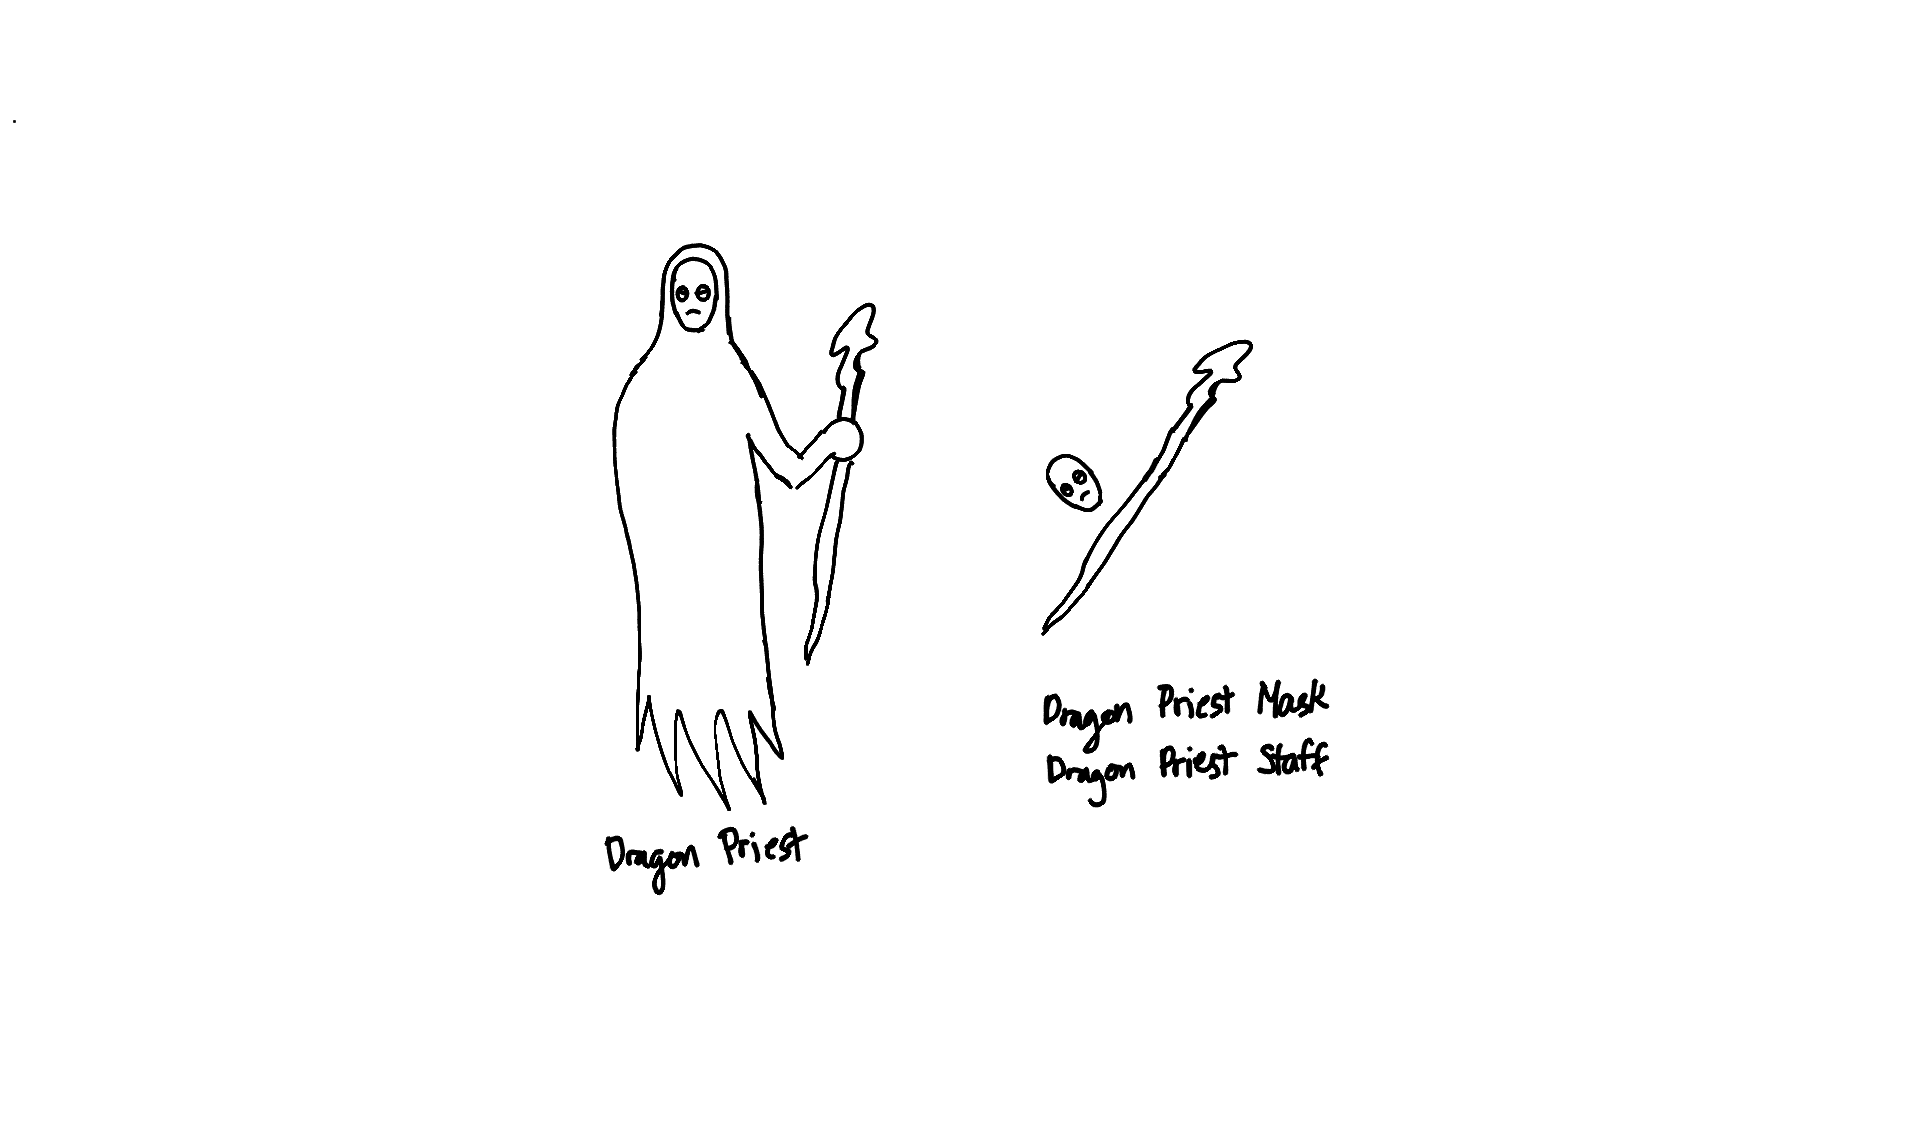
\includegraphics[keepaspectratio]{https://raw.githubusercontent.com/HowDoIGitHelp/CMSC23MDNotes/master/Markdown\%20Lecture\%20Notes\%20and\%20Lab\%20Exercises/copyright\%20free\%20drawings/DependencyRelationship.png}}
\caption{Dependency Example}
\end{figure}

\subsection{Aggregation}\label{class-relationships.md__aggregation}

Aggregation relationships are general usage and transactional
dependencies. When a dependency is an aggregate of some client, it means
that the client merely \textbf{uses} the instances of this dependency.
These relationships are the looser forms of dependency, because the
dependency instance can exist outside the lifetime of the client
instance.

For example, in a videogame, a hostile enemy instance of
\texttt{DragonPriest} spawns equipped with instances
of\texttt{DragonPriestMask} and \texttt{DragonPriestStaff}. The
\texttt{DragonPriest} instance is a client of the dependencies
\texttt{DragonPriestMask} and \texttt{DragonPriestStaff}.
\texttt{DragonPriest} interacts with these dependencies to calculate its
attack damage, its defenses and etc. But when this specific instance of
\texttt{DragonPriest} is defeated, it despawns, leaving behind the its
\texttt{DragonPriestMask} and \texttt{DragonPriestStaff}. These
instances will continue to exist since it can still be used by other
client objects in the game, such as the player character, some storage
chest or whatever. This means that the relationship between
\texttt{DragonPriest} and the dependencies \texttt{DragonPriestMask} and
\texttt{DragonPriestStaff} is aggregation.

\subsection{Composition}\label{class-relationships.md__composition}

Composition relationships are ownership dependencies. When a client is
composed of some dependency, this means that the client \textbf{owns}
the instances of this dependency. These relationships are stronger forms
of dependency since the existence of the dependency instance is tied to
the client, meaning, the dependency ceases to exist outside the lifetime
of the client instance.

In the same videogame, the hostile enemy instance of
\texttt{DragonPriest} appears in game using some
\texttt{DragonPriestCharacterModel} instance. When the
\texttt{DragonPriest} instance is defeated, it despawns. It makes no
sense for the \texttt{DragonPriestCharacterModel} instance to stay
behind after the \texttt{DragonPriest} instance is defeated, therefore
it ceases to exist as well. This means that the relationship between
\texttt{DragonPriest} and the dependency
\texttt{DragonPriestCharacterModel} is composition.

\chapter{OOPython}\label{oopython.md__oopython}

\section{Introduction}\label{oopython.md__introduction}

Python was never originally meant for pure oop. But OOP is not a
classification, it is a paradigm. The language does not make the OOP
elegant, it's how you adhere to the design principles of the paradigm.

\section{Learning Outcomes}\label{oopython.md__learning-outcomes}

\begin{enumerate}
\def\labelenumi{\arabic{enumi}.}
\tightlist
\item
  Create python classes and objects/instances
\item
  Create \texttt{\_\_init\_\_()} methods
\item
  Establish realization relationships in python
\item
  Establish specialization relationships in python
\item
  Explain how different levels of visibility affects access and
  inheritance in python
\end{enumerate}

\begin{center}\rule{0.5\linewidth}{0.5pt}\end{center}

\section{Python Classes}\label{oopython.md__python-classes}

Creating classes in python is very easy, here's an empty class called
\texttt{EmptyClass}:

\begin{quote}
In python and other OOP languages, naming classes with nouns that start
with capital letters is a convention. You can name it with weird names
but correct naming is good practice for maintainability.
\end{quote}

\begin{Shaded}
\begin{Highlighting}[]
\KeywordTok{class}\NormalTok{ EmptyClass:}
    \ControlFlowTok{pass}
\end{Highlighting}
\end{Shaded}

You write \texttt{pass} to indicate that this specific scope is empty.
By putting \texttt{pass} inside classes the classes will have no
attributes or methods, thus an empty class.

To make this class more interesting, lets put something inside it. You
can put methods and attributes inside classes. Everything found inside
the indent level of a class, belongs to that class.

\begin{Shaded}
\begin{Highlighting}[]
\ImportTok{from}\NormalTok{ abc }\ImportTok{import}\NormalTok{ ABC, abstractmethod}

\KeywordTok{class}\NormalTok{ EmptyClass:}
    \ControlFlowTok{pass}

\KeywordTok{class}\NormalTok{ VoiceBox:}
\NormalTok{    name : }\BuiltInTok{str} \OperatorTok{=} \StringTok{"Vincent"}
    \KeywordTok{def}\NormalTok{ speak():}
        \BuiltInTok{print}\NormalTok{(}\StringTok{"Hi, I\textquotesingle{}m "} \OperatorTok{+}\NormalTok{ VoiceBox.name }\OperatorTok{+} \StringTok{" the VoiceBox"}\NormalTok{)}

\NormalTok{VoiceBox.speak()}
\NormalTok{VoiceBox.name }\OperatorTok{=} \StringTok{"Vito"}
\NormalTok{VoiceBox.speak()}
\end{Highlighting}
\end{Shaded}

\begin{verbatim}
Hi, I'm Vincent the VoiceBox
Hi, I'm Vito the VoiceBox
\end{verbatim}

When the \texttt{VoiceBox.speak()} is called, the method
\texttt{speak()} found inside the scope of \texttt{VoiceBox} is called.
This function accesses an a identifier called \texttt{VoiceBox.name}
which refers to the identifier \texttt{name} found inside
\texttt{VoiceBox}. As, you can see, classes in python uses dot-reference
similar to C.

When \texttt{VoiceBox.name\ =\ "Vito"} is executed, it changes the
assigned value to ``Vito (which was originally''Vincent''). Now when
\texttt{VoiceBox.speak()} is invoked again, it says ``Hi, I'm Vito the
VoiceBox''.

This usage of classes is not actually interesting at all. Even though it
contains attributes and methods, this class is merely used like a data
holder. The attributes and methods you see inside \texttt{VoiceBox}
right now are what we call \textbf{static} attributes and
\textbf{static} methods. We won't really use a lot of static attributes
and methods in this course (it's not good practice to use them).
Basically, statics are attributes and methods that are not associated to
class instances. They exist in the class itself, outside the lifetime of
any instance.

Right now, the \texttt{VoiceBox} class is unable to create meaningful
instances or objects. To do that we need to implement a constructor.
Let's make a new class, one that can construct meaningful instances of
itself.

\section{\texorpdfstring{\texttt{\_\_init\_\_()}
Constructor}{\_\_init\_\_() Constructor}}\label{oopython.md__init__-constructor}

The \texttt{\_\_init\_\_()} method is a special method that is
responsible for spawning instances of the class. This method stands for
\textbf{initialization}. Here it is in action.

\begin{quote}
\texttt{\_\_init\_\_} is surrounded by two underscores on each side.
\end{quote}

\begin{Shaded}
\begin{Highlighting}[]
\KeywordTok{class}\NormalTok{ Robot:}
    \KeywordTok{def} \FunctionTok{\_\_init\_\_}\NormalTok{(}\VariableTok{self}\NormalTok{, n : }\BuiltInTok{str}\NormalTok{):}
        \VariableTok{self}\NormalTok{.name }\OperatorTok{=}\NormalTok{ n}

    \KeywordTok{def}\NormalTok{ talk(}\VariableTok{self}\NormalTok{):}
        \BuiltInTok{print}\NormalTok{(}\StringTok{"Howdy, it\textquotesingle{}s me, "}\OperatorTok{+} \VariableTok{self}\NormalTok{.name)}

    \KeywordTok{def}\NormalTok{ communicate(}\VariableTok{self}\NormalTok{, partner : }\StringTok{\textquotesingle{}Robot\textquotesingle{}}\NormalTok{):}
        \BuiltInTok{print}\NormalTok{(}\StringTok{"Howdy, "}\OperatorTok{+}\NormalTok{ partner.name }\OperatorTok{+} \StringTok{" it\textquotesingle{}s me, "}\OperatorTok{+} \VariableTok{self}\NormalTok{.name )}

\NormalTok{r1 : Robot }\OperatorTok{=}\NormalTok{ Robot(}\StringTok{"Bonk"}\NormalTok{)}
\NormalTok{r2 : Robot }\OperatorTok{=}\NormalTok{ Robot(}\StringTok{"Chonk"}\NormalTok{)}

\NormalTok{r1.talk()}
\NormalTok{r2.talk()}

\NormalTok{r1.name }\OperatorTok{=} \StringTok{"Donk"}

\NormalTok{r2.communicate(r1)}
\end{Highlighting}
\end{Shaded}

\begin{verbatim}
Howdy, it's me, Bonk
Howdy, it's me, Chonk
Howdy, Donk it's me, Chonk
\end{verbatim}

Lets look at this code piece by piece. First the \texttt{\_\_init\_\_()}
method

\begin{Shaded}
\begin{Highlighting}[]
\CommentTok{\#Robot}
\KeywordTok{def} \FunctionTok{\_\_init\_\_}\NormalTok{(}\VariableTok{self}\NormalTok{, n : }\BuiltInTok{str}\NormalTok{):}
    \VariableTok{self}\NormalTok{.name }\OperatorTok{=}\NormalTok{ n}
\end{Highlighting}
\end{Shaded}

Here you'll notice a special identifier called \texttt{self}. The
identifier \texttt{self} is a special reference to the instance of the
class using this. Basically whichever instance is being spawned right
now is assigned to \texttt{self}. It doesn't actually have to be named
\texttt{self} you can name it anything (but naming it \texttt{self} is a
python convention). Python understands that the first identifier found
at any non-static method is a reference to the instance invoking the
method.

Inside, we are preparing the instance by assigning values to its
attributes. We do that by assigning \texttt{n}, a string type parameter
passed to \texttt{\_\_init\_\_()}, to \texttt{self.name}. Since name is
dot referenced to \texttt{self}, which is the instance being spawned,
the instance gains the \texttt{name} attribute. Unlike,
\texttt{VoiceBox.name}, this attribute is associated to an instance of
\texttt{Robot} not the class \texttt{Robot} itself.

There's also something not explicitly shown here that python
automatically does. The method \texttt{\_\_init\_\_()} returns
\texttt{self}, the instance being spawned at the by
\texttt{\_\_init\_\_()}.

To use the \texttt{\_\_init\_\_()} function, we create two instances of
\texttt{Robot} using the following code:

\begin{Shaded}
\begin{Highlighting}[]
\CommentTok{\#outside Robot}
\NormalTok{r1 : Robot }\OperatorTok{=}\NormalTok{ Robot(}\StringTok{"Bonk"}\NormalTok{)}
\NormalTok{r2 : Robot }\OperatorTok{=}\NormalTok{ Robot(}\StringTok{"Chonk"}\NormalTok{)}
\end{Highlighting}
\end{Shaded}

The identifier \texttt{r1} is assigned a new instance of \texttt{Robot}
named ``Bonk'', and the identifier \texttt{r2} is assigned a new
instance of \texttt{Robot} named ``Chonk''.

The expression \texttt{Robot("Bonk")} is equivalent to the invoking the
\texttt{\_\_init\_\_()} function, while passing the string ``Bonk'' to
be assigned to the parameter \texttt{n}. Notice how
\texttt{\_\_init\_\_()} expects two parameters but its invocation
\texttt{Robot("Bonk")} only provides two, that is because the instance
assigned to \texttt{self} is automatically passed without being
explicitly shown (take note of this because a lot of people forget about
the hidden \texttt{self}, including me from time to time).

\begin{Shaded}
\begin{Highlighting}[]
\CommentTok{\#outside Robot}
\NormalTok{r1.talk()}
\NormalTok{r2.talk()}
\end{Highlighting}
\end{Shaded}

\begin{verbatim}
Howdy, it's me, Bonk
Howdy, it's me, Chonk
\end{verbatim}

Since there are two separate instances of \texttt{Robot} with different
names, it prints two different lines. This happens because inside of
what we wrote inside the method \texttt{talk()}

\begin{Shaded}
\begin{Highlighting}[]
\CommentTok{\#outside Robot}
\KeywordTok{def}\NormalTok{ talk(}\VariableTok{self}\NormalTok{):}
    \BuiltInTok{print}\NormalTok{(}\StringTok{"Howdy, it\textquotesingle{}s me, "}\OperatorTok{+} \VariableTok{self}\NormalTok{.name)}
\end{Highlighting}
\end{Shaded}

Notice how \texttt{talk()} uses the special reference \texttt{self}
again. \texttt{self} which is the first and only parameter passed, is
used by concatenating \texttt{self.name} to the printed message. Since
\texttt{self} refers to the instance invoking talk, the instance's own
name is used (``Bonk'' for \texttt{r1} and ``Chonk'' for \texttt{r2}).

Also, notice how when invoked, nothing is passed to \texttt{talk()},
despite expecting one parameter. This is again because the instance
invoking, is automatically passed and assigned to \texttt{self} behind
the scenes.

\begin{quote}
When you're writing a non-static method, always include \texttt{self}.
Even if you do not use the reference to \texttt{self} inside the
function. That's because python will force the first parameter in the
method to accept the instance reference.
\end{quote}

Let's look at the next lines of code.

\begin{Shaded}
\begin{Highlighting}[]
\CommentTok{\#outside Robot}

\NormalTok{r1.name }\OperatorTok{=} \StringTok{"Donk"}

\NormalTok{r2.communicate(r1)}
\end{Highlighting}
\end{Shaded}

\begin{verbatim}
Howdy, Donk it's me, Chonk
\end{verbatim}

First, the name of the instance assigned to \texttt{r1} is changed from
``Bonk'' to ``Donk''. Then, \texttt{r2} invokes its method
\texttt{communicate()} passing the instance \texttt{r1}. Let's look at
the insides of \texttt{communicate()}.

\begin{Shaded}
\begin{Highlighting}[]
\CommentTok{\#inside Robot}
\KeywordTok{def}\NormalTok{ communicate(}\VariableTok{self}\NormalTok{, partner : }\StringTok{\textquotesingle{}Robot\textquotesingle{}}\NormalTok{):}
    \BuiltInTok{print}\NormalTok{(}\StringTok{"Howdy, "}\OperatorTok{+}\NormalTok{ partner.name }\OperatorTok{+} \StringTok{" it\textquotesingle{}s me, "}\OperatorTok{+} \VariableTok{self}\NormalTok{.name )}
\end{Highlighting}
\end{Shaded}

The instance assigned to \texttt{r1} is passed and assigned to
\texttt{Robot}. The instance \texttt{r2} is also passed and assigned to
\texttt{self} but behind the scenes. Inside this method both
\texttt{partner.name} and \texttt{self.name} are used. \texttt{partner}
refers to the instance named ``Donk'' and \texttt{self} refers to the
invoker of the method, the one named ``Chonk''. As, a resilt of all
these, the line ``Howdy, Donk it's me, Chonk'' is printed.

\begin{quote}
If you notice the type annotation \texttt{Robot} is surrounded by single
quotes. If you remove these quotes, python will spill an error because
it doesn't recognize an \texttt{Robot} as a class name yet. That's
because the \texttt{communicate()} function is inside \texttt{Robot},
therefore Robot hasn't been defined yet.
\end{quote}

\section{Python Realizations and
Specializations}\label{oopython.md__python-realizations-and-specializations}

\subsection{Specialization}\label{oopython.md__specialization}

The syntax for establishing realization and specialization relationships
are the same in python. It just depends if the classes involved are
abstractions or generalizations.

Here's a generalization relationship in action.

\begin{Shaded}
\begin{Highlighting}[]
\KeywordTok{class}\NormalTok{ SkyBot(Robot):}
    \KeywordTok{def}\NormalTok{ fly(}\VariableTok{self}\NormalTok{, height:}\BuiltInTok{int}\NormalTok{):}
        \BuiltInTok{print}\NormalTok{(}\StringTok{"I\textquotesingle{}m "}\OperatorTok{+} \BuiltInTok{str}\NormalTok{(height) }\OperatorTok{+}\StringTok{"m high in the air. Skybot go zoom. "}\NormalTok{)}

\NormalTok{r3:SkyBot }\OperatorTok{=}\NormalTok{ SkyBot(}\StringTok{"Zonk"}\NormalTok{)}
\NormalTok{r3.talk()}
\NormalTok{r3.fly(}\DecValTok{3}\NormalTok{)}
\end{Highlighting}
\end{Shaded}

\begin{verbatim}
Howdy, it's me, Zonk
I'm 3m high in the air. Skybot go zoom.
\end{verbatim}

\begin{quote}
Note how even though, \texttt{self} is unused inside the method
\texttt{fly()}, \texttt{self} is written in the parameter list. If you
do not do that, the python will assign the invoking instance to
\texttt{height}.
\end{quote}

\begin{quote}
Since \texttt{height} is \texttt{int} you need to convert it using the
\texttt{str()} function so that concatenation is allowed.
\end{quote}

The class \texttt{SkyBot} becomes a specialization of \texttt{Robot}
through the line, \texttt{class\ SkyBot(Robot):}. The class name between
the parentheses will be specialized by the class outside the
parentheses.

\begin{figure}
\centering
\pandocbounded{\includesvg[keepaspectratio]{uml/robots.svg}}
\caption{robot relationships}
\end{figure}

Notice how even though the functions \texttt{\_\_init\_\_()},
\texttt{talk()}, and \texttt{communicate()} are not in found in the
scope of \texttt{SkyBot}, you are still able to use them. That is
because \texttt{SkyBot} has inherited them.

\begin{quote}
If class relationships haven't been discussed yet. Don't worry we will
talk about them in a future lecture. For this lecture focus on python
syntax.
\end{quote}

Here's an example that shows how to extend the attributes of a
generalization

\begin{Shaded}
\begin{Highlighting}[]
\KeywordTok{class}\NormalTok{ ShadeBot(Robot):}
    \KeywordTok{def} \FunctionTok{\_\_init\_\_}\NormalTok{(}\VariableTok{self}\NormalTok{, n:}\BuiltInTok{str}\NormalTok{, o:}\BuiltInTok{float}\NormalTok{):}
\NormalTok{        Robot.}\FunctionTok{\_\_init\_\_}\NormalTok{(}\VariableTok{self}\NormalTok{,n)}
        \VariableTok{self}\NormalTok{.visorOpacity }\OperatorTok{=}\NormalTok{ o}

    \KeywordTok{def}\NormalTok{ communicate(}\VariableTok{self}\NormalTok{,partner:Robot):}
        \ControlFlowTok{if} \VariableTok{self}\NormalTok{.visorOpacity }\OperatorTok{\textgreater{}=} \DecValTok{1}\NormalTok{:}
            \BuiltInTok{print}\NormalTok{(}\StringTok{"Howdy, it\textquotesingle{}s me, "}\OperatorTok{+} \VariableTok{self}\NormalTok{.name }\OperatorTok{+} \StringTok{". Sorry I cant see you my shades are too dark"}\NormalTok{)}
        \ControlFlowTok{else}\NormalTok{:}
            \BuiltInTok{print}\NormalTok{(}\StringTok{"Howdy, "}\OperatorTok{+}\NormalTok{ partner.name }\OperatorTok{+} \StringTok{" it\textquotesingle{}s me, "}\OperatorTok{+} \VariableTok{self}\NormalTok{.name)}

\NormalTok{r4:ShadeBot }\OperatorTok{=}\NormalTok{ ShadeBot(}\StringTok{"Tonk"}\NormalTok{, }\DecValTok{1}\NormalTok{)}
\NormalTok{r4.talk()}
\NormalTok{r4.communicate(r3)}
\end{Highlighting}
\end{Shaded}

\begin{verbatim}
Howdy, it's me, Tonk
Howdy, it's me, Tonk. Sorry I cant see you my shades are too dark
\end{verbatim}

Here, even though \texttt{ShadeBot} inherits \texttt{\_\_init\_\_} from
\texttt{Robot}, it has its own definition of \texttt{\_\_init\_\_}. When
this is done, \texttt{ShadeBot} replaces \texttt{Robot}'s version of
\texttt{\_\_init\_\_} with its own. This is called \textbf{method
overriding}. You will need to do this for \texttt{\_\_init\_\_} if you
need to extend the class to have more attributes (You also override
methods if you need something changed for the specializations). We are
doing this for \texttt{ShadeBot} since we need to add the attribute
\texttt{visorOpacity}.

You'll notice the strange line of code,
\texttt{Robot.\_\_init\_\_(self,n)} inside \texttt{Shadebot}'s
\texttt{\_\_init\_\_}. What you're doing here is statically invoking
\texttt{Robot}'s \texttt{\_\_init\_\_} function to reuse the code inside
it (statically invoking means that the class itself is invoking the
method not any instance, that's why \texttt{self} is being explicitly
passed). Calling this is similar to doing the following

\begin{Shaded}
\begin{Highlighting}[]
\CommentTok{\#ShadeBot}
\KeywordTok{def} \FunctionTok{\_\_init\_\_}\NormalTok{(}\VariableTok{self}\NormalTok{, n:}\BuiltInTok{str}\NormalTok{, o:}\BuiltInTok{float}\NormalTok{):}
    \VariableTok{self}\NormalTok{.name }\OperatorTok{=}\NormalTok{ n}
    \VariableTok{self}\NormalTok{.visorOpacity }\OperatorTok{=}\NormalTok{ o}
\end{Highlighting}
\end{Shaded}

If you're not changing anything that happens during the
\texttt{\_\_init\_\_} of the specialization just extending it, then you
can statically invoke the generalization's \texttt{\_\_init\_\_}.
Otherwise, if you need to change how the specialization gets its name
for example, then you have to fully write the whole specialization's
\texttt{\_\_init\_\_}.

\begin{Shaded}
\begin{Highlighting}[]
\CommentTok{\#ShadeBot}
\KeywordTok{def} \FunctionTok{\_\_init\_\_}\NormalTok{(}\VariableTok{self}\NormalTok{, n:}\BuiltInTok{str}\NormalTok{, o:}\BuiltInTok{float}\NormalTok{):}
    \VariableTok{self}\NormalTok{.name }\OperatorTok{=} \StringTok{"Mr."} \OperatorTok{+}\NormalTok{ n}
    \VariableTok{self}\NormalTok{.visorOpacity }\OperatorTok{=}\NormalTok{ o}
\end{Highlighting}
\end{Shaded}

\section{Realization}\label{oopython.md__realization}

The syntax for realization is just the same as specialization. If you
put an abstraction inside the parentheses then the relationship becomes
realization.

\begin{Shaded}
\begin{Highlighting}[]
\ImportTok{from}\NormalTok{ abc }\ImportTok{import}\NormalTok{ ABC, abstractmethod}

\KeywordTok{class}\NormalTok{ BorrowableItem(ABC):}
    \AttributeTok{@abstractmethod}
    \KeywordTok{def}\NormalTok{ borrow(}\VariableTok{self}\NormalTok{):}
        \ControlFlowTok{pass}

    \AttributeTok{@abstractmethod}
    \KeywordTok{def}\NormalTok{ name(}\VariableTok{self}\NormalTok{) }\OperatorTok{{-}\textgreater{}} \BuiltInTok{str}\NormalTok{:}
        \ControlFlowTok{pass}

\KeywordTok{class}\NormalTok{ Book(BorrowableItem):}
    \KeywordTok{def} \FunctionTok{\_\_init\_\_}\NormalTok{(}\VariableTok{self}\NormalTok{, title:}\BuiltInTok{str}\NormalTok{):}
        \VariableTok{self}\NormalTok{.title }\OperatorTok{=}\NormalTok{ title}

    \KeywordTok{def}\NormalTok{ borrow(}\VariableTok{self}\NormalTok{):}
        \BuiltInTok{print}\NormalTok{(}\StringTok{"I\textquotesingle{}m a book called "}\OperatorTok{+} \VariableTok{self}\NormalTok{.name() }\OperatorTok{+}\StringTok{" and I\textquotesingle{}m being borrowed"}\NormalTok{)}

    \KeywordTok{def}\NormalTok{ name(}\VariableTok{self}\NormalTok{) }\OperatorTok{{-}\textgreater{}} \BuiltInTok{str}\NormalTok{:}
        \ControlFlowTok{return} \VariableTok{self}\NormalTok{.title}

\KeywordTok{class}\NormalTok{ IMacUnit(BorrowableItem):}
    \KeywordTok{def} \FunctionTok{\_\_init\_\_}\NormalTok{(}\VariableTok{self}\NormalTok{, }\BuiltInTok{id}\NormalTok{:}\BuiltInTok{int}\NormalTok{):}
        \VariableTok{self}\NormalTok{.}\BuiltInTok{id} \OperatorTok{=} \BuiltInTok{id}

    \KeywordTok{def}\NormalTok{ borrow(}\VariableTok{self}\NormalTok{):}
        \BuiltInTok{print}\NormalTok{(}\StringTok{"I\textquotesingle{}m an iMac called "}\OperatorTok{+} \VariableTok{self}\NormalTok{.name() }\OperatorTok{+}\StringTok{" and I\textquotesingle{}m being borrowed"}\NormalTok{)}

    \KeywordTok{def}\NormalTok{ name(}\VariableTok{self}\NormalTok{) }\OperatorTok{{-}\textgreater{}} \BuiltInTok{str}\NormalTok{:}
        \ControlFlowTok{return} \StringTok{"iMac"} \OperatorTok{+} \BuiltInTok{str}\NormalTok{(}\VariableTok{self}\NormalTok{.}\BuiltInTok{id}\NormalTok{)}


\NormalTok{b : BorrowableItem }\OperatorTok{=}\NormalTok{ Book(}\StringTok{"Necronomicon"}\NormalTok{)}
\NormalTok{i : BorrowableItem }\OperatorTok{=}\NormalTok{ IMacUnit(}\DecValTok{5}\NormalTok{)}

\NormalTok{b.borrow()}
\NormalTok{i.borrow()}
\end{Highlighting}
\end{Shaded}

\begin{verbatim}
I'm a book called Necronomicon and I'm being borrowed
I'm an iMac called iMac5 and I'm being borrowed
\end{verbatim}

First things first, to be able to make use of abstractions, you need to
import the \texttt{abc} library. We specifically need 2 things, the
class \texttt{ABC} which stands for \textbf{abstract base class} and the
decorator \texttt{abstractmethod}. You typically put import lines at the
top of your code, above everything else.

\begin{figure}
\centering
\pandocbounded{\includesvg[keepaspectratio]{uml/OOPythonLib.svg}}
\caption{realization uml}
\end{figure}

The abstraction in this case is the class called
\texttt{BorrowableItem}. For a class to become an abstraction it needs
to realize the imported class \texttt{ABC}, hence the line
\texttt{class\ BorrowableItem(ABC):}.

Inside \texttt{BorrowableItem} are two methods called \texttt{borrow()}
and \texttt{name()}. Both of these methods are decorated by
\texttt{@abstracmethod}. You see this decoration above all methods that
you want to be abstracted. Inside each of \texttt{borrow()} and
\texttt{name()} is the special expression \texttt{pass}. Which means
that these methods are empty. They do not contain any implementation or
body. You can put code inside these methods but it wouldn't matter since
these methods will be guaranteed to be overwritten by
\texttt{BorrowableItem}'s realizations.

What \texttt{@abstractmethod} does is, it indicate to python that the
directly method below it, must be overridden by the abstraction's
realizations. You'll notice this if you change the code above by adding
another method decorated with \texttt{@abstractmethod} without
implementing it inside all the realizations, you'll get the following
error during instantiation:

\begin{Shaded}
\begin{Highlighting}[]
\CommentTok{\#BorrowableItem}
\AttributeTok{@abstractmethod}
\KeywordTok{def}\NormalTok{ implementationRequirement(}\VariableTok{self}\NormalTok{):}
    \ControlFlowTok{pass}
\end{Highlighting}
\end{Shaded}

\begin{verbatim}
Traceback (most recent call last):
  File ".\OOPython.py", line 95, in <module>
    b : BorrowableItem = Book("Necronomicon")
TypeError: Can't instantiate abstract class Book with abstract methods implementationRequirement
\end{verbatim}

Without \texttt{@abstractmethod} python will not complain

\begin{Shaded}
\begin{Highlighting}[]
\CommentTok{\#BorrowableItem}
\KeywordTok{def}\NormalTok{ implementationRequirement(}\VariableTok{self}\NormalTok{):}
    \ControlFlowTok{pass}
\end{Highlighting}
\end{Shaded}

\begin{verbatim}
I'm a book called Necronomicon and I'm being borrowed
I'm an iMac called iMac5 and I'm being borrowed
\end{verbatim}

The decorator \texttt{@abstractmethod} reminds all realizations of the
requirements to remind any class that realizes the abstraction, ``hey
these are the functions that you need to be considered a
\texttt{BorrowableItem}''.

Moving on to the realizations, you see is that each realization
overrides all abstract methods. You can also put methods that are not
found in the abstraction. Here, you see both of them contain an
\texttt{\_\_init\_\_()} method for instantiation.

\begin{quote}
Note on the code inside \texttt{Book}`s \texttt{\_\_init\_\_()}':
although the parameter is called \texttt{title} and the attribute is
called \texttt{title} as well, python can differentiate between them
since the instance's title has to be dot referenced as
\texttt{self.title} while the non-dot referenced \texttt{title} can only
mean the parameter. It's fine to this, especially if you want to
emphasize which parameters are stored to which attributes. In fact, I do
this quite a lot.
\end{quote}

\begin{quote}
Note how the abstraction \texttt{BorrowableItem} does not contain an
\texttt{\_\_init\_\_()} method. This is because he
\texttt{BorrowableItem} is not meant to be spawned/instantiated. It is
merely an abstraction so it must be ethereal and formless.
\end{quote}

Outside the class scopes you'll see these borrowable items instantiated
like these:

\begin{Shaded}
\begin{Highlighting}[]
\NormalTok{b : BorrowableItem }\OperatorTok{=}\NormalTok{ Book(}\StringTok{"Necronomicon"}\NormalTok{)}
\NormalTok{i : BorrowableItem }\OperatorTok{=}\NormalTok{ IMacUnit(}\DecValTok{5}\NormalTok{)}
\end{Highlighting}
\end{Shaded}

Both \texttt{b} and \texttt{i} are annotated to be of type
\texttt{BorrowableItem} but they are instantiated from \texttt{Book} and
\texttt{IMacUnit}. This is allowed because of polymorphism. Through
realization, instances of \texttt{Book} and \texttt{IMacUnit} can be
treated as \texttt{BorrowableItem}'s (they can also be treated
specifically as \texttt{Book} and \texttt{IMacUnit}).

\section{Python Visibility
Control}\label{oopython.md__python-visibility-control}

Another important python syntax to remember is how to simulate different
visibility levels for methods and attributes. Given the following class
below, notice how the attributes and methods have special prefixes.
These prefixes tell you that their visibility level.

\begin{Shaded}
\begin{Highlighting}[]
\KeywordTok{class}\NormalTok{ ClandestineClass:}
    \KeywordTok{def} \FunctionTok{\_\_init\_\_}\NormalTok{(}\VariableTok{self}\NormalTok{, publicValue:}\BuiltInTok{int}\NormalTok{, protectedValue:}\BuiltInTok{int}\NormalTok{, privateValue:}\BuiltInTok{int}\NormalTok{):}
        \VariableTok{self}\NormalTok{.publicValue }\OperatorTok{=}\NormalTok{ publicValue}
        \VariableTok{self}\NormalTok{.\_protectedValue }\OperatorTok{=}\NormalTok{ protectedValue}
        \VariableTok{self}\NormalTok{.\_\_privateValue }\OperatorTok{=}\NormalTok{ privateValue}


    \KeywordTok{def}\NormalTok{ doPublicly(}\VariableTok{self}\NormalTok{):}
        \BuiltInTok{print}\NormalTok{(}\StringTok{"Hey!, these are my values"}\NormalTok{)}
        \BuiltInTok{print}\NormalTok{(}\VariableTok{self}\NormalTok{.publicValue)}
        \BuiltInTok{print}\NormalTok{(}\VariableTok{self}\NormalTok{.\_protectedValue)}
        \BuiltInTok{print}\NormalTok{(}\VariableTok{self}\NormalTok{.\_\_privateValue)}

    \KeywordTok{def}\NormalTok{ \_doProtectedly(}\VariableTok{self}\NormalTok{):}
        \BuiltInTok{print}\NormalTok{(}\StringTok{"hey"}\NormalTok{)}

    \KeywordTok{def}\NormalTok{ \_\_doPrivately(}\VariableTok{self}\NormalTok{):}
        \BuiltInTok{print}\NormalTok{(}\StringTok{"..."}\NormalTok{)}
\end{Highlighting}
\end{Shaded}

When the following code is ran, you'll notice that private, attributes
and methods are not recognized by python:

\begin{Shaded}
\begin{Highlighting}[]
\CommentTok{\#outside ClandestineClass}
\BuiltInTok{print}\NormalTok{(c.publicValue)}
\BuiltInTok{print}\NormalTok{(c.\_protectedValue)}
\BuiltInTok{print}\NormalTok{(c.\_\_privateValue)}
\end{Highlighting}
\end{Shaded}

\begin{verbatim}
1
2
Traceback (most recent call last):
  File ".\OOPython.py", line 122, in <module>
    print(c.__privateValue)
\end{verbatim}

In other oop based languages, protected values are not supposed to be
accessible outside the class. But python doesn't have this mechanism.
What python programmers do instead is to write protected identifiers
with a single underscore prefix. Yes you can access them but you are not
supposed to.

Of course all of these attributes can be accessed \textbf{inside} the
class:

\begin{Shaded}
\begin{Highlighting}[]
\NormalTok{c.doPublicly()}
\end{Highlighting}
\end{Shaded}

\begin{verbatim}
Hey!, these are my values
1
2
3
\end{verbatim}

Specializations do not have access to the private attributes and methods
of its generalizations. . But both public and protected are. If you want
some attributes/methods to be inherited but still (sort-of) inaccessible
outside, make them protected instead.

\begin{Shaded}
\begin{Highlighting}[]
\KeywordTok{class}\NormalTok{ SpecialClandestineClass(ClandestineClass):}
    \KeywordTok{def}\NormalTok{ doSomethingSpecial(}\VariableTok{self}\NormalTok{):}
        \BuiltInTok{print}\NormalTok{(}\VariableTok{self}\NormalTok{.publicValue)}
        \BuiltInTok{print}\NormalTok{(}\VariableTok{self}\NormalTok{.\_protectedValue)}
        \BuiltInTok{print}\NormalTok{(}\VariableTok{self}\NormalTok{.\_\_privateValue)}

\NormalTok{s:SpecialClandestineClass }\OperatorTok{=}\NormalTok{ SpecialClandestineClass(}\DecValTok{1}\NormalTok{,}\DecValTok{2}\NormalTok{,}\DecValTok{3}\NormalTok{)}
    
\NormalTok{s.doPublicly()}
\BuiltInTok{print}\NormalTok{() }\CommentTok{\#prints a new line for formatting}
\NormalTok{s.doSomethingSpecial()}
\end{Highlighting}
\end{Shaded}

\begin{verbatim}
Hey!, these are my values
1
2
3

1
2
Traceback (most recent call last):
  File ".\OOPython.py", line 133, in <module>
    s.doSomethingSpecial()
  File ".\OOPython.py", line 123, in doSomethingSpecial
    print(self.__privateValue)
AttributeError: 'SpecialClandestineClass' object has no attribute '_SpecialClandestineClass__privateValue'
\end{verbatim}

Note how \texttt{s.doPublicly()} still works perfectly because its
definition lies inside \texttt{ClandestineClass}. On the other hand,
\texttt{s.doSomethingSpecial()} will fail in printing private values
since it is outside \texttt{ClandestineClass}.

Here's a summary of the access rules.

\begin{longtable}[]{@{}
  >{\raggedright\arraybackslash}p{(\linewidth - 6\tabcolsep) * \real{0.0893}}
  >{\raggedright\arraybackslash}p{(\linewidth - 6\tabcolsep) * \real{0.2143}}
  >{\raggedright\arraybackslash}p{(\linewidth - 6\tabcolsep) * \real{0.2143}}
  >{\raggedright\arraybackslash}p{(\linewidth - 6\tabcolsep) * \real{0.4821}}@{}}
\toprule\noalign{}
\begin{minipage}[b]{\linewidth}\raggedright
visibility
\end{minipage} & \begin{minipage}[b]{\linewidth}\raggedright
prefix
\end{minipage} & \begin{minipage}[b]{\linewidth}\raggedright
accessed specializations
\end{minipage} & \begin{minipage}[b]{\linewidth}\raggedright
accessed by clients
\end{minipage} \\
\midrule\noalign{}
\endhead
\bottomrule\noalign{}
\endlastfoot
public & (none) & yes & yes \\
protected & \texttt{\_} (single underscore) & yes & technically yes in
python (but you're not supposed to) \\
private & \texttt{\_\_} (double underscore) & no & no \\
\end{longtable}

\begin{quote}
Private values in python can actually be accessed outside using a
special syntax. But it is out of scope here and you're not supposed to
this anyway so don't worry about it.
\end{quote}

\section{Abstract Classes}\label{oopython.md__abstract-classes}

Abstract classes in python are implemented similar to how Abstractions
are implemented. All methods that you want to be implemented are
decorated by \texttt{@abstractmethod} while all methods you want to be
inherited are not decorated.

\begin{Shaded}
\begin{Highlighting}[]
\KeywordTok{class}\NormalTok{ AbstractClass(ABC):}
    \AttributeTok{@abstractmethod}
    \KeywordTok{def}\NormalTok{ printSomethingA(}\VariableTok{self}\NormalTok{):}
        \ControlFlowTok{pass}

    \KeywordTok{def}\NormalTok{ printSomethingB(}\VariableTok{self}\NormalTok{):}
        \BuiltInTok{print}\NormalTok{(}\StringTok{"I\textquotesingle{}m inherited. You can also override me if you want"}\NormalTok{)}

\KeywordTok{class}\NormalTok{ ConcreteClass1(AbstractClass):}
    \KeywordTok{def}\NormalTok{ printSomethingA(}\VariableTok{self}\NormalTok{):}
        \BuiltInTok{print}\NormalTok{(}\StringTok{"I\textquotesingle{}m implemented by Concrete Class 1"}\NormalTok{)}

\KeywordTok{class}\NormalTok{ ConcreteClass2(AbstractClass):}
    \KeywordTok{def}\NormalTok{ printSomethingA(}\VariableTok{self}\NormalTok{):}
        \BuiltInTok{print}\NormalTok{(}\StringTok{"I\textquotesingle{}m implemented by Concrete Class 2"}\NormalTok{)}

    \KeywordTok{def}\NormalTok{ printSomethingB(}\VariableTok{self}\NormalTok{):}
        \BuiltInTok{print}\NormalTok{(}\StringTok{"I\textquotesingle{}m overriden by Concrete Class 2"}\NormalTok{)}
\end{Highlighting}
\end{Shaded}

Both \texttt{ConcreteClass1} and \texttt{ConcreteClass2} are
realizations/specializations of \texttt{AbstractClass} therefore they
must implement \texttt{printSomethingA()} otherwise it will cause an
error (because of the \texttt{@abstractmethod} decoration). The other
method \texttt{printSomethingB()} will automatically be inherited by
both, but can still be optionally overridden (\texttt{ConcreteClass2}
does this).

\begin{Shaded}
\begin{Highlighting}[]
\CommentTok{\#outside the classes}
\NormalTok{c1.printSomethingA()}
\NormalTok{c1.printSomethingB()}
\BuiltInTok{print}\NormalTok{()}
\NormalTok{c2.printSomethingA()}
\NormalTok{c2.printSomethingB()}
\end{Highlighting}
\end{Shaded}

\begin{verbatim}
I'm implemented by Concrete Class 1
I'm inherited. You can also override me if you want

I'm implemented by Concrete Class 2
I'm overriden by Concrete Class 2
\end{verbatim}

\chapter{Unified Modelling Language for Class
Diagrams}\label{unified-modelling-language-for-class-diagrams.md__unified-modelling-language-for-class-diagrams}

\section{Introduction}\label{unified-modelling-language-for-class-diagrams.md__introduction}

The modelling language we are going to use to represent architecture
would be UML or \textbf{Unified Modelling Language}. We use this to show
the relevant classes in the system including their attributes, methods
and relationships with other classes. UML differ a little depending on
the source. The specifications we'll be following in this class would be
based on PlantUML.

\section{Learning
Outcomes}\label{unified-modelling-language-for-class-diagrams.md__learning-outcomes}

\begin{enumerate}
\def\labelenumi{\arabic{enumi}.}
\tightlist
\item
  Create class diagrams to represent OOP architecture in UML

  \begin{enumerate}
  \def\labelenumii{\arabic{enumii}.}
  \tightlist
  \item
    Create classes with attributes and methods in UML
  \item
    Establish class relationships in UML
  \end{enumerate}
\end{enumerate}

\begin{center}\rule{0.5\linewidth}{0.5pt}\end{center}

\section{Modelling
Classes}\label{unified-modelling-language-for-class-diagrams.md__modelling-classes}

The example below shows three classes. One is concrete class called
\texttt{ExampleClass} (notice the ``C'' in the title that denotes it is
a concrete class). Another is an abstraction called
\texttt{ExampleAbstraction} (denoted by ``I'' which stands for
interface). The last one is \texttt{ExampleAbstractClass} which is an
abstract class (denoted by ``A'').

\begin{figure}
\centering
\pandocbounded{\includesvg[keepaspectratio]{https://raw.githubusercontent.com/HowDoIGitHelp/CMSC23MDNotes/master/Markdown\%20Lecture\%20Notes\%20and\%20Lab\%20Exercises/uml/classExample.svg}}
\caption{Class Diagrams}
\end{figure}

Attributes are placed in the top portion and methods are placed in the
bottom portion. The shape to the left of each attribute or method
indicates its visibility. Filled shapes indicate visibilities for
methods while unfilled shapes indicate visibilities for attributes.

\begin{quote}
When writing UML for python code, I usually omit writing the
\texttt{self} special identifier inside method specifications. It is
implied that \texttt{self} is passed always for all non-static methods
in python.
\end{quote}

\begin{longtable}[]{@{}
  >{\centering\arraybackslash}p{(\linewidth - 4\tabcolsep) * \real{0.4615}}
  >{\centering\arraybackslash}p{(\linewidth - 4\tabcolsep) * \real{0.4615}}
  >{\centering\arraybackslash}p{(\linewidth - 4\tabcolsep) * \real{0.0769}}@{}}
\toprule\noalign{}
\begin{minipage}[b]{\linewidth}\centering
attribute
\end{minipage} & \begin{minipage}[b]{\linewidth}\centering
method
\end{minipage} & \begin{minipage}[b]{\linewidth}\centering
visibility
\end{minipage} \\
\midrule\noalign{}
\endhead
\bottomrule\noalign{}
\endlastfoot
\pandocbounded{
\includegraphics[keepaspectratio]{https://raw.githubusercontent.com/HowDoIGitHelp/CMSC23MDNotes/master/Markdown\%20Lecture\%20Notes\%20and\%20Lab\%20Exercises/uml/private-field.png}}
&
\pandocbounded{
\includegraphics[keepaspectratio]{https://raw.githubusercontent.com/HowDoIGitHelp/CMSC23MDNotes/master/Markdown\%20Lecture\%20Notes\%20and\%20Lab\%20Exercises/uml/private-method.png}}
& private \\
\pandocbounded{
\includegraphics[keepaspectratio]{https://raw.githubusercontent.com/HowDoIGitHelp/CMSC23MDNotes/master/Markdown\%20Lecture\%20Notes\%20and\%20Lab\%20Exercises/uml/protected-field.png}}
&
\pandocbounded{
\includegraphics[keepaspectratio]{https://raw.githubusercontent.com/HowDoIGitHelp/CMSC23MDNotes/master/Markdown\%20Lecture\%20Notes\%20and\%20Lab\%20Exercises/uml/protected-method.png}}
& protected \\
\pandocbounded{
\includegraphics[keepaspectratio]{https://raw.githubusercontent.com/HowDoIGitHelp/CMSC23MDNotes/master/Markdown\%20Lecture\%20Notes\%20and\%20Lab\%20Exercises/uml/public-field.png}}
&
\pandocbounded{
\includegraphics[keepaspectratio]{https://raw.githubusercontent.com/HowDoIGitHelp/CMSC23MDNotes/master/Markdown\%20Lecture\%20Notes\%20and\%20Lab\%20Exercises/uml/public-method.png}}
& public \\
\end{longtable}

The names for abstract methods, abstractions, and abstract classes are
italicized.

If possible, write the expected type of attributes, parameters and
function returns. This is written on the right side of their names, to
the right of ``:''.

\begin{quote}
\textbf{Disclaimer}: sometimes you'll find some mistakes in my uml
diagrams, sometimes I write the incorrect visibility marker or neglect
abstract italicizations. Rest assured the code will contain the correct
visibility markers, abstract modifiers and etc.
\end{quote}

\section{Modelling Class
Relationships}\label{unified-modelling-language-for-class-diagrams.md__modelling-class-relationships}

Here's a reference arrows that indicate the relationship between two
classes:

\begin{figure}
\centering
\pandocbounded{\includesvg[keepaspectratio]{https://raw.githubusercontent.com/HowDoIGitHelp/CMSC23MDNotes/master/Markdown\%20Lecture\%20Notes\%20and\%20Lab\%20Exercises/uml/classRelationships.svg}}
\caption{class relationships}
\end{figure}

\begin{quote}
Sometimes, instead of writing the specific kind of dependency arrow
(aggregation or composition), I just write the general dependency arrow
instead
\end{quote}

\section{Optional
Readings}\label{unified-modelling-language-for-class-diagrams.md__optional-readings}

PlantUML Class Diagrams. https://plantuml.com/class-diagram Accessed
August 31, 2020

\chapter{Exceptions}\label{exceptions.md__exceptions}

\section{Introduction}\label{exceptions.md__introduction}

One of the features added to imperative programming was the elegant
handling of errors. Exception handling provided OOP a mechanism to
control what exactly the system does when parts of the system fail.

\section{Learning Outcomes}\label{exceptions.md__learning-outcomes}

\begin{enumerate}
\def\labelenumi{\arabic{enumi}.}
\tightlist
\item
  Create methods that raise errors in python
\item
  Create a try-except clause to properly react to errors in python
\item
  Design systems that correctly assign error handling responsibilties
\end{enumerate}

\begin{center}\rule{0.5\linewidth}{0.5pt}\end{center}

Let's explore this with an example. In the snippet below, the last line
is not reached because the system fails during
\texttt{print(quotientUnsafe(3,0))}.

\begin{Shaded}
\begin{Highlighting}[]
\KeywordTok{def}\NormalTok{ quotientUnsafe(a:}\BuiltInTok{float}\NormalTok{, b:}\BuiltInTok{float}\NormalTok{) }\OperatorTok{{-}\textgreater{}} \BuiltInTok{float}\NormalTok{:}
    \ControlFlowTok{return}\NormalTok{ a}\OperatorTok{/}\NormalTok{b}

\BuiltInTok{print}\NormalTok{(quotientUnsafe(}\DecValTok{3}\NormalTok{,}\DecValTok{2}\NormalTok{))}
\BuiltInTok{print}\NormalTok{(quotientUnsafe(}\DecValTok{3}\NormalTok{,}\DecValTok{0}\NormalTok{))}
\BuiltInTok{print}\NormalTok{(}\StringTok{"some more behavior"}\NormalTok{)}
\end{Highlighting}
\end{Shaded}

\begin{Shaded}
\begin{Highlighting}[]
\FloatTok{1.5}
\OperatorTok{{-}{-}{-}{-}{-}{-}{-}{-}{-}{-}{-}{-}{-}{-}{-}{-}{-}{-}{-}{-}{-}{-}{-}{-}{-}{-}{-}{-}{-}{-}{-}{-}{-}{-}{-}{-}{-}{-}{-}{-}{-}{-}{-}{-}{-}{-}{-}{-}{-}{-}{-}{-}{-}{-}{-}{-}{-}{-}{-}{-}{-}{-}{-}{-}{-}{-}{-}{-}{-}{-}{-}{-}{-}{-}{-}}
\PreprocessorTok{ZeroDivisionError}\NormalTok{                         Traceback (most recent call last)}
 \KeywordTok{in} 
      \DecValTok{3} 
      \DecValTok{4} \BuiltInTok{print}\NormalTok{(quotientUnsafe(}\DecValTok{3}\NormalTok{,}\DecValTok{2}\NormalTok{))}
\OperatorTok{{-}{-}{-}{-}\textgreater{}} \DecValTok{5} \BuiltInTok{print}\NormalTok{(quotientUnsafe(}\DecValTok{3}\NormalTok{,}\DecValTok{0}\NormalTok{))}
      \DecValTok{6} \BuiltInTok{print}\NormalTok{(}\StringTok{"some more behavior"}\NormalTok{)}

 \KeywordTok{in}\NormalTok{ quotientUnsafe(a, b)}
      \DecValTok{1} \KeywordTok{def}\NormalTok{ quotientUnsafe(a:}\BuiltInTok{float}\NormalTok{, b:}\BuiltInTok{float}\NormalTok{) }\OperatorTok{{-}\textgreater{}} \BuiltInTok{float}\NormalTok{:}
\OperatorTok{{-}{-}{-}{-}\textgreater{}} \DecValTok{2}     \ControlFlowTok{return}\NormalTok{ a}\OperatorTok{/}\NormalTok{b}
      \DecValTok{3} 
      \DecValTok{4} \BuiltInTok{print}\NormalTok{(quotientUnsafe(}\DecValTok{3}\NormalTok{,}\DecValTok{2}\NormalTok{))}
      \DecValTok{5} \BuiltInTok{print}\NormalTok{(quotientUnsafe(}\DecValTok{3}\NormalTok{,}\DecValTok{0}\NormalTok{))}

\PreprocessorTok{ZeroDivisionError}\NormalTok{: division by zero}
\end{Highlighting}
\end{Shaded}

\begin{quote}
Python has its own error raised when it encounter division by zero but
well create our own for the sake of learning
\end{quote}

Problematic functions and methods like \texttt{quotientUnsafe} don't
always return a float. The problem for this \texttt{quotientUnsafe}
function is that there is a possibility you'll end up dividing with
zero. This introduces the concept of exception. Where the quotient
function works \textbf{except} when the denominator is zero.

To implement this kind of behavior. You create an if-else check (or any
control statement) to make sure the denominator is not zero. If you do
encounter a zero denominator you \textbf{\texttt{raise}} an error. Here
you are raising a user defined error object called
\texttt{DivisionByZeroError}.

\begin{Shaded}
\begin{Highlighting}[]
\KeywordTok{class}\NormalTok{ DivisionByZeroError(}\PreprocessorTok{Exception}\NormalTok{):}
    \KeywordTok{def} \FunctionTok{\_\_init\_\_}\NormalTok{(}\VariableTok{self}\NormalTok{,numerator:}\BuiltInTok{float}\NormalTok{, denominator:}\BuiltInTok{float}\NormalTok{):}
        \VariableTok{self}\NormalTok{.numerator }\OperatorTok{=}\NormalTok{ numerator}
        \VariableTok{self}\NormalTok{.denominator }\OperatorTok{=}\NormalTok{ denominator}

\KeywordTok{def}\NormalTok{ quotient(a:}\BuiltInTok{float}\NormalTok{, b:}\BuiltInTok{float}\NormalTok{) }\OperatorTok{{-}\textgreater{}} \BuiltInTok{float}\NormalTok{: }\CommentTok{\#maybe a float}
    \ControlFlowTok{if}\NormalTok{ b }\OperatorTok{==} \DecValTok{0}\NormalTok{:}
        \ControlFlowTok{raise}\NormalTok{ DivisionByZeroError(a,b)}
    \ControlFlowTok{else}\NormalTok{:}
        \ControlFlowTok{return}\NormalTok{ a}\OperatorTok{/}\NormalTok{b}
\end{Highlighting}
\end{Shaded}

When quotient is called where the denominator passed is zero, python
will inform you that the function call has resulted in a
\texttt{DivisionByZeroError}

\begin{Shaded}
\begin{Highlighting}[]
\ControlFlowTok{try}\NormalTok{:}
\NormalTok{    quotient(}\DecValTok{3}\NormalTok{,}\DecValTok{2}\NormalTok{)}
\NormalTok{    quotient(}\DecValTok{3}\NormalTok{,}\DecValTok{0}\NormalTok{)}
\ControlFlowTok{except}\NormalTok{ DivisionByZeroError:}
    \BuiltInTok{print}\NormalTok{(}\StringTok{"there was dividing by zero somewhere but it\textquotesingle{}s okay I\textquotesingle{}m still fine"}\NormalTok{)}
    
\BuiltInTok{print}\NormalTok{(}\StringTok{"some more behavior"}\NormalTok{)}
\end{Highlighting}
\end{Shaded}

\begin{verbatim}
there was dividing by zero somewhere but it's okay I'm still fine
some more behavior
\end{verbatim}

By enclosing the lines of code that could potentially raise errors, you
create a safety net for the system. The system \textbf{tries} to execute
these lines, and if there are no errors raised inside the \texttt{try}
block then the system runs normally. Nothing abnormal would occur
\textbf{except} when the problematic lines of code raises an error. In
this specific case, the system is catching, a specific type of error
called \texttt{DivisionByZeroError}. If a specific type of error is not
specified in the exception block, the system will catch any general
error.

If a method with potential to raise errors like \texttt{quotient()}, is
invoked inside another method without using the try except block, the
caller method becomes a method with potential to raise errors as well.

\begin{Shaded}
\begin{Highlighting}[]
\KeywordTok{def}\NormalTok{ mixedFraction(a:}\BuiltInTok{float}\NormalTok{, b: }\BuiltInTok{float}\NormalTok{, c:}\BuiltInTok{float}\NormalTok{) }\OperatorTok{{-}\textgreater{}} \BuiltInTok{float}\NormalTok{: }\CommentTok{\#maybe a float}
    \ControlFlowTok{return}\NormalTok{ a }\OperatorTok{+}\NormalTok{ quotient(b,c)}

\NormalTok{mixedFraction(}\DecValTok{1}\NormalTok{,}\DecValTok{1}\NormalTok{,}\DecValTok{0}\NormalTok{)}
\BuiltInTok{print}\NormalTok{(}\StringTok{"some more behavior"}\NormalTok{)}
\end{Highlighting}
\end{Shaded}

\begin{Shaded}
\begin{Highlighting}[]
\OperatorTok{{-}{-}{-}{-}{-}{-}{-}{-}{-}{-}{-}{-}{-}{-}{-}{-}{-}{-}{-}{-}{-}{-}{-}{-}{-}{-}{-}{-}{-}{-}{-}{-}{-}{-}{-}{-}{-}{-}{-}{-}{-}{-}{-}{-}{-}{-}{-}{-}{-}{-}{-}{-}{-}{-}{-}{-}{-}{-}{-}{-}{-}{-}{-}{-}{-}{-}{-}{-}{-}{-}{-}{-}{-}{-}{-}}
\NormalTok{DivisionByZeroError                       Traceback (most recent call last)}
 \KeywordTok{in}\NormalTok{ ()}
      \DecValTok{2}     \ControlFlowTok{return}\NormalTok{ a }\OperatorTok{+}\NormalTok{ quotient(b,c)}
      \DecValTok{3} 
\OperatorTok{{-}{-}{-}{-}\textgreater{}} \DecValTok{4}\NormalTok{ mixedFraction(}\DecValTok{1}\NormalTok{,}\DecValTok{1}\NormalTok{,}\DecValTok{0}\NormalTok{)}

 \KeywordTok{in}\NormalTok{ mixedFraction(a, b, c)}
      \DecValTok{1} \KeywordTok{def}\NormalTok{ mixedFraction(a:}\BuiltInTok{float}\NormalTok{, b: }\BuiltInTok{float}\NormalTok{, c:}\BuiltInTok{float}\NormalTok{) }\OperatorTok{{-}\textgreater{}} \BuiltInTok{float}\NormalTok{: }\CommentTok{\#maybe a float}
\OperatorTok{{-}{-}{-}{-}\textgreater{}} \DecValTok{2}     \ControlFlowTok{return}\NormalTok{ a }\OperatorTok{+}\NormalTok{ quotient(b,c)}
      \DecValTok{3} 
      \DecValTok{4}\NormalTok{ mixedFraction(}\DecValTok{1}\NormalTok{,}\DecValTok{1}\NormalTok{,}\DecValTok{0}\NormalTok{)}

 \KeywordTok{in}\NormalTok{ quotient(a, b)}
      \DecValTok{7} \KeywordTok{def}\NormalTok{ quotient(a:}\BuiltInTok{float}\NormalTok{, b:}\BuiltInTok{float}\NormalTok{) }\OperatorTok{{-}\textgreater{}} \BuiltInTok{float}\NormalTok{: }\CommentTok{\#maybe a float}
      \DecValTok{8}     \ControlFlowTok{if}\NormalTok{ b }\OperatorTok{==} \DecValTok{0}\NormalTok{:}
\OperatorTok{{-}{-}{-}{-}\textgreater{}} \DecValTok{9}         \ControlFlowTok{raise}\NormalTok{ DivisionByZeroError(a,b)}
     \DecValTok{10}     \ControlFlowTok{else}\NormalTok{:}
     \DecValTok{11}         \ControlFlowTok{return}\NormalTok{ a}\OperatorTok{/}\NormalTok{b}

\NormalTok{DivisionByZeroError: (}\DecValTok{1}\NormalTok{, }\DecValTok{0}\NormalTok{)}
\end{Highlighting}
\end{Shaded}

Here, the \texttt{quotient()}'s caller,\texttt{mixedFraction()}, does
not enclose the problematic line with a try-except block. This means
that \texttt{mixedFraction} is basically the ignoring any potential
error, shifting the responsibility of dealing with the error to wherever
\texttt{mixedFraction()} is called.

On the example below, \texttt{quotient()} is invoked inside
\texttt{quotientString()}, but instead of ignoring the error,
\texttt{quotientString()} deals with it using a try-except block. When
quotient fails, the function returns ``undefined number'' instead of a
fraction string.

\begin{Shaded}
\begin{Highlighting}[]
\KeywordTok{def}\NormalTok{ quotientString(a:}\BuiltInTok{float}\NormalTok{,b:}\BuiltInTok{float}\NormalTok{) }\OperatorTok{{-}\textgreater{}} \BuiltInTok{str}\NormalTok{: }\CommentTok{\#always a string}
    \ControlFlowTok{try}\NormalTok{:}
\NormalTok{        wholePart }\OperatorTok{=}\NormalTok{ math.floor(quotient(a,b))}
\NormalTok{        decimalPart }\OperatorTok{=}\NormalTok{ quotient(a,b) }\OperatorTok{{-}}\NormalTok{ wholePart}
        \ControlFlowTok{return} \BuiltInTok{str}\NormalTok{(wholePart) }\OperatorTok{+} \StringTok{" and "} \OperatorTok{+} \BuiltInTok{str}\NormalTok{(decimalPart)}
    \ControlFlowTok{except} \PreprocessorTok{Exception}\NormalTok{:}
        \ControlFlowTok{return} \StringTok{"undefined number"}
\BuiltInTok{print}\NormalTok{(quotientString(}\DecValTok{17}\NormalTok{,}\DecValTok{7}\NormalTok{))}
\BuiltInTok{print}\NormalTok{(quotientString(}\DecValTok{1}\NormalTok{,}\DecValTok{0}\NormalTok{))}
\BuiltInTok{print}\NormalTok{(quotientString(}\DecValTok{1}\NormalTok{,}\DecValTok{3}\NormalTok{))}
\end{Highlighting}
\end{Shaded}

\begin{Shaded}
\begin{Highlighting}[]
\DecValTok{2} \KeywordTok{and} \FloatTok{0.4285714285714284}
\NormalTok{undefined number}
\DecValTok{0} \KeywordTok{and} \FloatTok{0.3333333333333333}
\end{Highlighting}
\end{Shaded}

By dealing with potential errors, \texttt{quotientString()} becomes a
safe function that has no potential of breaking the system.

You can catch multiple kinds of exceptions if you want to handle
different exceptions differently. The exception \texttt{IndexError} is
raised when an iterable type like list accesses a non-existent member.
Here the function \texttt{quotientList} wants to append
\texttt{math.inf} if you're dividing by zero and not append anything if
you're dividing with non-existent list members.

\begin{Shaded}
\begin{Highlighting}[]
\KeywordTok{def}\NormalTok{ quotientList(l:}\BuiltInTok{list}\NormalTok{[}\BuiltInTok{float}\NormalTok{],m:}\BuiltInTok{list}\NormalTok{[}\BuiltInTok{float}\NormalTok{]) }\OperatorTok{{-}\textgreater{}}\NormalTok{ [}\BuiltInTok{float}\NormalTok{]: }\CommentTok{\#always a list of float}
\NormalTok{    r }\OperatorTok{=}\NormalTok{ []}
    \ControlFlowTok{for}\NormalTok{ i }\KeywordTok{in} \BuiltInTok{range}\NormalTok{(}\DecValTok{0}\NormalTok{,}\BuiltInTok{len}\NormalTok{(l)):}
        \ControlFlowTok{try}\NormalTok{:}
\NormalTok{            r.append(quotient(l[i],m[i]))}
        \ControlFlowTok{except}\NormalTok{ DivisionByZeroError:}
\NormalTok{            r.append(math.inf)}
        \ControlFlowTok{except} \PreprocessorTok{IndexError}\NormalTok{:}
            \ControlFlowTok{pass}
    \ControlFlowTok{return}\NormalTok{ r}
\NormalTok{quotientList([}\DecValTok{1}\NormalTok{,}\DecValTok{2}\NormalTok{,}\DecValTok{3}\NormalTok{,}\DecValTok{4}\NormalTok{,}\DecValTok{5}\NormalTok{,}\DecValTok{6}\NormalTok{],[}\DecValTok{3}\NormalTok{,}\DecValTok{0}\NormalTok{,}\DecValTok{2}\NormalTok{,}\DecValTok{2}\NormalTok{,}\DecValTok{1}\NormalTok{])}
\end{Highlighting}
\end{Shaded}

\begin{Shaded}
\begin{Highlighting}[]
\NormalTok{quotientList([}\DecValTok{1}\NormalTok{,}\DecValTok{2}\NormalTok{,}\DecValTok{3}\NormalTok{,}\DecValTok{4}\NormalTok{,}\DecValTok{5}\NormalTok{,}\DecValTok{6}\NormalTok{],[}\DecValTok{3}\NormalTok{,}\DecValTok{0}\NormalTok{,}\DecValTok{2}\NormalTok{,}\DecValTok{2}\NormalTok{,}\DecValTok{1}\NormalTok{])}
\end{Highlighting}
\end{Shaded}

\subsection{To ignore errors or to deal with
errors?}\label{exceptions.md__to-ignore-errors-or-to-deal-with-errors}

So you've seen two ways to react with potential errors, to ignore them
like \texttt{mixedFraction()} or to deal with them like
\texttt{quotientString()}. Which is the proper way? You might think that
dealing with errors is better since it's this way doesn't break the
system. But actually the choice to ignore or to deal with errors depends
on who has the correct responsibility in fixing the error.

If you immediately deal with the error as quickly as possible, you'll
end up missing the importance of raising errors. The method
\texttt{quotient()} for example, is responsible for providing the caller
with a quotient, that must be this method's only responsibility. You
should not give \texttt{quotient} the responsibility of fixing division
by zeroes. That responsibility lies on its caller, because different
caller's may have different ways to deal with the error. The method
\texttt{quotientString()} deals with division by zero with ``undefined
number'' while the method \texttt{quotientList()} deals with division by
zero with ``inf''. These two callers have different ways of interpreting
division by zero so they should be the one's responsible for dealing
with the error.

\chapter{SOLID Objects}\label{solid-objects.md__solid-objects}

\section{Introduction}\label{solid-objects.md__introduction}

SOLID is an acronym describing design principles for creating OOP
systems. By committing your code to these principles you will naturally
build systems that don't only work perfectly, but work elegantly.

\section{Learning Outcomes}\label{solid-objects.md__learning-outcomes}

\begin{enumerate}
\def\labelenumi{\arabic{enumi}.}
\tightlist
\item
  Design methods and classes with exactly one responsibility
\item
  Design extension to classes to incorporate new behavior
\item
  Design proper realization and specialization relationships
\item
  Design purposeful abstractions and abstract methods
\item
  Design systems that interact through abstractions
\end{enumerate}

\begin{center}\rule{0.5\linewidth}{0.5pt}\end{center}

Briefly, these five principles are:

\begin{itemize}
\tightlist
\item
  \textbf{Single Responsibility Principle} - Objects should have
  cohesive and complete responsibilities. It shouldn't be aware of
  knowledge it doesn't need and it shouldn't perform responsibilities
  that are irrelevant from it.
\item
  \textbf{Open/Closed Principle} - Classes should be open to extension
  and closed to modification. Instead of changing the form and behavior
  of an existing class, you should extend the class
\item
  \textbf{Liskov-Substitution Principle} - Substituting objects by their
  subtypes/realizations should always work.
\item
  \textbf{Interface Segregation Principle} - A client shouldn't be
  forced to implement methods that it doesn't use
\item
  \textbf{Dependency Inversion Principle} - Object relationships should
  depend on abstractions instead of implementations
\end{itemize}

\subsection{Single Responsibility
Principle}\label{solid-objects.md__single-responsibility-principle}

\subsubsection{The GOD Class}\label{solid-objects.md__the-god-class}

One of the canonical examples of violations against SRP is the concept
known as the \textbf{god class}. A god class is a class that basically
contains all the attributes and methods of the whole system. You'll
recognize these god classes as those classes that control the behavior
of objects (they contain the implementation of client objects'
behavior). These god classes are also aware of all of the objects
secrets (they expose and manipulate private attributes and methods).

\begin{figure}
\centering
\pandocbounded{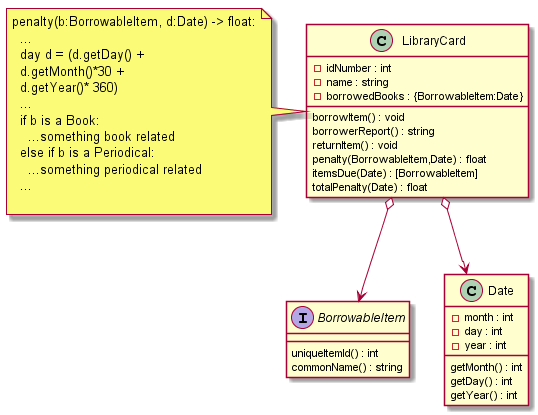
\includegraphics[keepaspectratio]{https://raw.githubusercontent.com/HowDoIGitHelp/CMSC23MDNotes/master/Markdown\%20Lecture\%20Notes\%20and\%20Lab\%20Exercises/uml/godclasslibrarycard.png}}
\caption{god class library card}
\end{figure}

On the example above \texttt{LibraryCard} is a god class since it
exposes the secrets of \texttt{Date} by forcing the creations of
\emph{evil} getters (\texttt{getMonth()}, \texttt{getDay()},
\texttt{getYear()}) for otherwise private details. Although it isn't
obvious, it also tampers on the responsibilities of
\texttt{BorrowableItem} by deciding by itself how penalty is calculated
for each realization.

\begin{quote}
The moment you ask an object what it's exact type is, you should
consider refactoring your code since introspective checks like
\texttt{isinstance} , \texttt{instanceof} \texttt{typeof} and etc., are
symptoms of smelly design. You can think of these checks as analogies to
racial discrimination since your client object asks the race (type) of
the dependency.
\end{quote}

\subsubsection{Assigning the correct
responsibilities}\label{solid-objects.md__assigning-the-correct-responsibilities}

When you're introducing new behavior or information to a system, you
should ask first: \emph{who should be responsible of this behavior or
information?}

\begin{itemize}
\tightlist
\item
  Who should be responsible of calculating the differences between
  dates? \textbf{\texttt{Date} should be responsible, not
  \texttt{LibraryCard}}.
\item
  Who should be responsible of calculating the penalties of specific
  \texttt{BorrowableItem} realizations? \textbf{\texttt{BorrowableItem}
  realizations should be responsible, not \texttt{LibraryCard}}
\end{itemize}

The best implementation of the system contains multiple examples of SRP.
The \texttt{Date} class should be responsible of subtracting dates and
adding dates, not the \texttt{LibraryCard} class. Forcing
\texttt{LibraryCard} to contain code for \texttt{Date} operations will
force you into breaking the boundaries of your classes (e.g.~creating
getters to expose private attributes). \texttt{LibraryCard} should not
be aware of \textbf{how} dates are subtracted to be able to subtract
dates. The same is true for a \texttt{BorrowableItem}'s due date. The
\texttt{LibraryCard} shouldn't contain the specifications as to how
\texttt{BorrowableItem}s calculate their due date. In fact
\texttt{LibraryCard} shouldn't even be aware of the exact type of the
\texttt{BorrowableItem} (\texttt{isinstance} violates this).

The process of designing these cohesive systems requires not only OOP
design techniques but also domain knowledge. The designer of the system,
should know how a library system operates so that, he/she can accurately
simulate their responsibilities on code.

You can also apply SRP on individual methods inside objects. Methods
should be responsible of one thing only. Keeping methods pure like these
will help reduce unwanted side effects. The builder/manipulator naming
scheme will help you with this. Also, a method should not be responsible
of handling the problems such as errors/exceptions. The method should
delegate that responsibility to the clients of that method. The methods
itself should only report/raise/throw the problem. The best way to do
this in OOP is by raising an exception.

\subsection{Open/Closed
Principle}\label{solid-objects.md__openclosed-principle}

A good class in OOP is both open and closed. It is open for extension
but closed for modification.

To understand this principle lets have an example of a system that is
closed for extension:

\begin{figure}
\centering
\pandocbounded{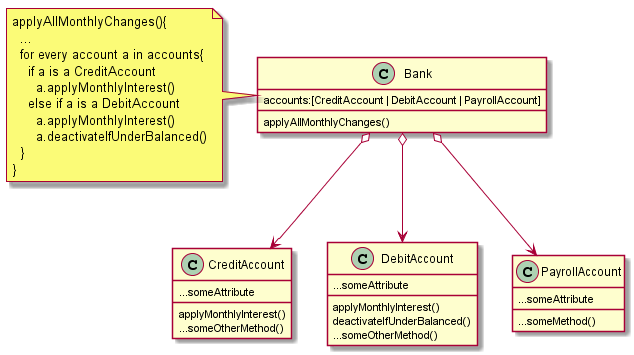
\includegraphics[keepaspectratio]{https://raw.githubusercontent.com/HowDoIGitHelp/CMSC23MDNotes/master/Markdown\%20Lecture\%20Notes\%20and\%20Lab\%20Exercises/uml/closedforextension.png}}
\caption{god class library card}
\end{figure}

\begin{quote}
Forgive the long Java-like method names, they're named as descriptive as
possible so that I can skip actually explaining what they do.
\end{quote}

This is a system that indeed works perfectly. The bank will be able to
apply the appropriate changes to the account types because of the
\texttt{if-else} block that segregates the accounts based on its type
(another instance of type discrimination so that's a hint that this is
bad design). The problem with this is that whenever there are changes
regarding the monthly changes or interest calculations, you would have
to tamper with the contents of bank. This is \textbf{opening
\texttt{Bank} up for modification}. Every time there's a change related
to monthly updates you would have to do some kind of surgical procedure
on \texttt{Bank} and rearrange its internal organs so that the change
may be supported. This is extra rough on \texttt{Bank} because
\texttt{Bank} shouldn't even be responsible for these behaviors (a
violation of SRP). If there are new types of account, then you would
have to open up \texttt{Bank} again and to add another \texttt{else\ if}
block. Poor \texttt{Bank}, who knows how many more new types of accounts
there are in the future.

Instead of rearranging the organs of your classes to accommodate changes
to behavior they are not even responsible for, you should close the
classes for modification and open them for extension instead:

\begin{figure}
\centering
\pandocbounded{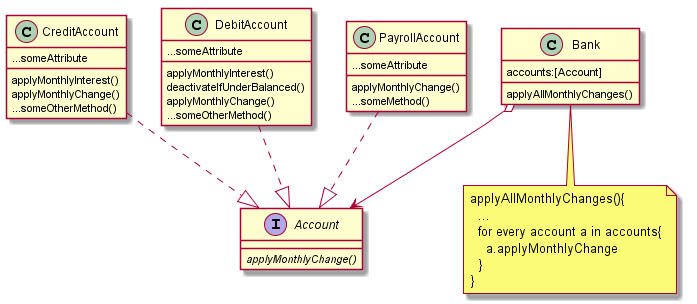
\includegraphics[keepaspectratio]{https://raw.githubusercontent.com/HowDoIGitHelp/CMSC23MDNotes/master/Markdown\%20Lecture\%20Notes\%20and\%20Lab\%20Exercises/uml/openforextension.png}}
\caption{open for extension}
\end{figure}

Since \texttt{applyMonthlyChange()} is an abstract method of account,
all its realizations are required to implement it. We extend the
functionality of \texttt{CreditAccount}, \texttt{DebitAccount}, and
\texttt{PayrollAccount} by adding an extra method.

\begin{itemize}
\tightlist
\item
  inside \texttt{CreditAccount.applyMonthlyChange()} you just call
  \texttt{applyMonthlyInterest()},\\
\item
  inside \texttt{DebitAccount.applyMonthlyChange()} you call both
  \texttt{applyMontlyInterest()} and
  \texttt{deactivateIfUnderBalanced()}
\item
  inside \texttt{PayrollAccount.applyMonthlyChange()} you do nothing
\end{itemize}

Is a method that does nothing inelegant? Not really because this is an
accurate representation as to how a \texttt{PayrollAccount} changes
every month--- it doesn't change. Also, in the future, the inertness of
\texttt{PayrollAccount} may change so at least you have the function
prepared.

\begin{quote}
The previous library card example and bank examples are indeed similar .
This is because introspective checks like \texttt{isinstance} are again
symptoms of inelegant design.
\end{quote}

Another example of this is how you need to augment the
\texttt{PayrollAccount} class to contain the \texttt{recieveFund(float)}
or \texttt{deposit(float)} method so that it can become a recipient for
transfer.

\begin{quote}
Closed for modification does not mean you cannot change literally
anything in the class. Of course if there are mistakes in the specific
behavior of the class then you have to modify it.
\end{quote}

\subsection{Liskov-Substitution
Principle}\label{solid-objects.md__liskov-substitution-principle}

This principle basically dictates when should an object be a subtype or
a realization of another object. Should \texttt{PayrollAccount} be a
realization of \texttt{Account}? If you can substitute any instance of
an \texttt{Account}with a \texttt{PayrollAccount} then the answer is
yes. The same is true if you want to establish an inheritance
relationship between \texttt{Account} and \texttt{PayrollAccount}. LSP
is important because it ensures the polymorphic capabilities of your
realizations and subtypes.

\subsection{Interface Segregation
Principle}\label{solid-objects.md__interface-segregation-principle}

Sometimes the subtypes/realizations of a certain object may have diverse
functionality. Some subtypes can deposit, some subtypes can't, all
subtypes can be recipient for transfers but not all can be senders. The
diversity of functionality support may sometimes force the designer to
pollute the system with methods that the subtypes don't actually use.
\texttt{PayrollAccount} will not use deposit but since it realizes
\texttt{Account} then we reluctantly add it. This is a violation if LSP
which states that an object should not be forced to implement methods it
doesn't use.

\subsubsection{Role Interfaces}\label{solid-objects.md__role-interfaces}

The best way to design these diverse systems it by refactoring your
architecture to have diverse role interfaces instead.

\begin{figure}
\centering
\pandocbounded{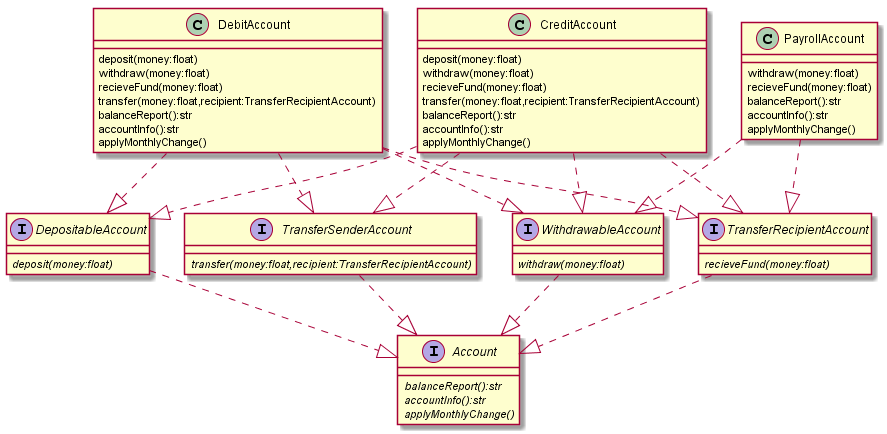
\includegraphics[keepaspectratio]{https://raw.githubusercontent.com/HowDoIGitHelp/CMSC23MDNotes/master/Markdown\%20Lecture\%20Notes\%20and\%20Lab\%20Exercises/uml/roleinterfaces.png}}
\caption{god class library card}
\end{figure}

Now instead of cluttering you realizations with useless methods, your
systems is now cluttered with role interfaces. This is a benevolent kind
of clutter. Because more objects and looser dependencies make for a
maintainable and therefore elegant system (in the same way a language
with more words have less chances for ambiguity). Because of this
clutter, you can have rich polymorphism without sacrificing ISP.
Although be careful not to overdo it though. You wouldn't want a role
interface for every conceivable method out there.

When you have role interfaces, you can refine lines of your code by
describing which exact role interface applies. For example, instead of
writing \texttt{transfer} to be an process which is \texttt{Account} to
\texttt{Account} they are \texttt{TransferSenderAccount} to
\texttt{TransferRecipientAccount}.

\subsection{Dependency Inversion
Principle}\label{solid-objects.md__dependency-inversion-principle}

The relationships between objects should be defined by surface instead
of their interior. This means that How a bank interacts with an account
should not be dependent on the implementation. The way \texttt{Bank}
prints the balance report should not be by directly concatenating
\texttt{"Your\ balance\ is"\ \ +\ account.balance} . Bank should
interact with an account by printing the return value the abstract
builder method, \texttt{balanceReport()}. The class \texttt{Bank} should
not dissect an \texttt{Account} to retrieve the balance. It should tell
the \texttt{Account} to build a balance report.

\section{Optional Reading}\label{solid-objects.md__optional-reading}

Bailey D., (2009)
\href{https://lostechies.com/derickbailey/2009/02/11/solid-development-principles-in-motivational-pictures/}{SOLID
Development Principles -- In Motivational Pictures}. Accessed August 31,
2020

\chapter{Extra Stuff}\label{extra-stuff.md__extra-stuff}

Here are extra things I want to discuss that do not really fall into
specific lectures.

\section{Naming Methods
Elegantly}\label{extra-stuff.md__naming-methods-elegantly}

One of the important things to consider about coding in OOP (and in
general) is properly naming identifiers, functions, and classes. I'm
sure this was talked about in your early programming languages. Creating
names is a programming skill in and of itself. Creating concise (unlike
Java's verbose naming schemes), descriptive names help in the
maintainability of the code you're writing. When the name itself tells
you what an identifier is for and when the name of the modifier tells
you what it does, then you don't need to explain it in documentation or
comments.

Since you're probably experts in naming identifiers from you C coding
experience, lets focus on naming methods.

\begin{quote}
\textbf{Disclaimer}: These naming conventions are according to MY
standards of code elegance. I'm not saying that this particular way of
naming is the correct way, to be honest these standards are more
subjective than objective. While your in my course I hope you'll at
least try incorporate these conventions in your code. I don't care about
how you write names in other course, but in my course, these are the
names that I consider to be \emph{beautiful}.

Sometimes, even I forget to adhere to my own conventions, especially
when I'm writing code outside OOP. You'll probably notice some
contradictions to these conventions somewhere in this course. Just
consider these contradictions as proof that the instructor that made
these resources is indeed a human being. Let me offer you a preemptive
\emph{whoops} for all of those contradictions.
\end{quote}

Methods (and functions in general) can be divided into two types,
methods that return something, known as \textbf{builders}, and methods
that do not return something, known as \textbf{manipulators}.

\subsection{Builders}\label{extra-stuff.md__builders}

An inelegant method name:

\begin{Shaded}
\begin{Highlighting}[]
\KeywordTok{def}\NormalTok{ add(addend1:}\BuiltInTok{int}\NormalTok{, addend2:}\BuiltInTok{int}\NormalTok{) }\OperatorTok{{-}\textgreater{}} \BuiltInTok{int}\NormalTok{:}
    \ControlFlowTok{return}\NormalTok{ addend1 }\OperatorTok{+}\NormalTok{ addend2}
\end{Highlighting}
\end{Shaded}

Now this seems like a descriptive enough name that describes what the
method does. What is wrong with it? The issues start to surface once you
invoke the function:

\begin{Shaded}
\begin{Highlighting}[]
\NormalTok{solution }\OperatorTok{=} \DecValTok{5} \OperatorTok{{-}}\NormalTok{ add(}\DecValTok{3}\NormalTok{,}\DecValTok{2}\NormalTok{)}
\end{Highlighting}
\end{Shaded}

When you see this line of code, your brain reads this as:

``solution becomes five minus add three and two''

Which can still be understood since we're used to what the method
\texttt{add()} usually means. But consider this alternative way of
naming this function:

\begin{Shaded}
\begin{Highlighting}[]
\KeywordTok{def} \BuiltInTok{sum}\NormalTok{(addend1:}\BuiltInTok{int}\NormalTok{, addend2:}\BuiltInTok{int}\NormalTok{) }\OperatorTok{{-}\textgreater{}} \BuiltInTok{int}\NormalTok{:}
    \ControlFlowTok{return}\NormalTok{ addend1 }\OperatorTok{+}\NormalTok{ addend2}
\end{Highlighting}
\end{Shaded}

When called:

\begin{Shaded}
\begin{Highlighting}[]
\NormalTok{solution }\OperatorTok{=} \DecValTok{5} \OperatorTok{{-}} \BuiltInTok{sum}\NormalTok{(}\DecValTok{3}\NormalTok{,}\DecValTok{2}\NormalTok{)}
\end{Highlighting}
\end{Shaded}

Your brain reads this as:

``solution becomes 5 minus sum of 3 and 2''

Which makes way more sense.

One of the most egregious violations to this convention is the naming of
\textbf{getter}. Like the following

\begin{Shaded}
\begin{Highlighting}[]
\CommentTok{\#inside some class}
\KeywordTok{def}\NormalTok{ getName(}\VariableTok{self}\NormalTok{):}
    \ControlFlowTok{return} \VariableTok{self}\NormalTok{.\_\_name}
\end{Highlighting}
\end{Shaded}

\begin{Shaded}
\begin{Highlighting}[]
\BuiltInTok{print}\NormalTok{(}\StringTok{"Hello "} \OperatorTok{+}\NormalTok{ p.getName())}
\end{Highlighting}
\end{Shaded}

Getter functions are usually created to reveal the values of private
attributes. First of all getters, are a bit evil and must be avoided as
much as possible since they violate the privacy of private attributes.
It's supposed to be a private attribute, other classes are not supposed
to access.

But sometimes exposing these attributes are needed. Sometimes, you don't
need to be able to change the value of the private attribute, you just
need to know its value. The best way to name a getter is the following.

\begin{Shaded}
\begin{Highlighting}[]
\CommentTok{\#inside some class}
\KeywordTok{def}\NormalTok{ name(}\VariableTok{self}\NormalTok{):}
    \ControlFlowTok{return} \VariableTok{self}\NormalTok{.\_\_name}
\end{Highlighting}
\end{Shaded}

\begin{Shaded}
\begin{Highlighting}[]
\BuiltInTok{print}\NormalTok{(}\StringTok{"Hello "} \OperatorTok{+}\NormalTok{ p.name())}
\end{Highlighting}
\end{Shaded}

People might complain, that \texttt{name()} and \texttt{\_\_name} are
ambiguous. But for me this ambiguity is fine since they end up meaning
the same thing. Plus, they will never be used interchangeably (maybe in
functional paradigm they may) because one is a method and the other is
an attribute.

So the rule of the thumb that you need to follow when you are naming
builders is the following, \textbf{A method that returns something (a
builder), should be named after a noun that describe what it is
returning.}

\subsubsection{Some more builders named
elegantly}\label{extra-stuff.md__some-more-builders-named-elegantly}

This is a factory method, which is responsible for building new
instances of a class called person. Therefore this method is called
\texttt{newPerson()}

\begin{Shaded}
\begin{Highlighting}[]
\CommentTok{\#inside some class}
\KeywordTok{def}\NormalTok{ newPerson(}\VariableTok{self}\NormalTok{) }\OperatorTok{{-}\textgreater{}}\NormalTok{ Person:}
    \ControlFlowTok{return}\NormalTok{ Person()}
\end{Highlighting}
\end{Shaded}

This method returns the element of a given list at position \(k\)

\begin{Shaded}
\begin{Highlighting}[]
\KeywordTok{def}\NormalTok{ kthElement(}\BuiltInTok{list}\NormalTok{:[}\BuiltInTok{float}\NormalTok{],k:}\BuiltInTok{int}\NormalTok{) }\OperatorTok{{-}\textgreater{}} \BuiltInTok{float}\NormalTok{:}
    \ControlFlowTok{return} \BuiltInTok{list}\NormalTok{[k]}
\end{Highlighting}
\end{Shaded}

This is a method that returns the concatenation of two strings

\begin{Shaded}
\begin{Highlighting}[]
\KeywordTok{def}\NormalTok{ concatenation(u:}\BuiltInTok{str}\NormalTok{, v: }\BuiltInTok{str}\NormalTok{) }\OperatorTok{{-}\textgreater{}} \BuiltInTok{str}\NormalTok{:}
    \ControlFlowTok{return}\NormalTok{ u }\OperatorTok{+}\NormalTok{ v}
\end{Highlighting}
\end{Shaded}

\subsection{Manipulators}\label{extra-stuff.md__manipulators}

This is an example of an inelegantly named manipulator:

\begin{Shaded}
\begin{Highlighting}[]
\CommentTok{\#inside some class}
\KeywordTok{def}\NormalTok{ nameString(}\VariableTok{self}\NormalTok{):}
    \BuiltInTok{print}\NormalTok{(}\VariableTok{self}\NormalTok{.\_\_name)}
\end{Highlighting}
\end{Shaded}

When your brain reads an invocation of this method it appears out of
place:

\begin{Shaded}
\begin{Highlighting}[]
\ControlFlowTok{if}\NormalTok{ (value }\OperatorTok{\textgreater{}}\NormalTok{ threshold):}
\NormalTok{    nameString()}
\ControlFlowTok{else}\NormalTok{:}
    \BuiltInTok{print}\NormalTok{(}\StringTok{"value is invalid"}\NormalTok{)}
\end{Highlighting}
\end{Shaded}

A better name for this function is the following:

\begin{Shaded}
\begin{Highlighting}[]
\CommentTok{\#inside some class}
\KeywordTok{def}\NormalTok{ printName(}\VariableTok{self}\NormalTok{):}
    \BuiltInTok{print}\NormalTok{(}\VariableTok{self}\NormalTok{.\_\_name)}
\end{Highlighting}
\end{Shaded}

\begin{Shaded}
\begin{Highlighting}[]
\ControlFlowTok{if}\NormalTok{ (value }\OperatorTok{\textgreater{}}\NormalTok{ threshold):}
\NormalTok{    p.printName()}
\ControlFlowTok{else}\NormalTok{:}
    \BuiltInTok{print}\NormalTok{(}\StringTok{"value is invalid"}\NormalTok{)}
\end{Highlighting}
\end{Shaded}

The original name \texttt{nameString()} is inelegant because it is named
like a builder, when in fact it doesn't build anything. It returns
nothing. This method an example of a \textbf{manipulator}. It should be
named like a manipulator. This particular method manipulates the output
stream of wherever you are printing.

\textbf{Setter} methods are actually named correctly, setter methods are
methods that set the value of a specific private attribute:

\begin{Shaded}
\begin{Highlighting}[]
\CommentTok{\#inside some class}
\KeywordTok{def}\NormalTok{ setName(}\VariableTok{self}\NormalTok{, newValue:}\BuiltInTok{str}\NormalTok{):}
    \VariableTok{self}\NormalTok{.\_\_name }\OperatorTok{=}\NormalTok{ newValue}
\end{Highlighting}
\end{Shaded}

Setters are also quite evil in the same way getters are evil. These
methods change the values of private methods, violating their privacy.
Although the usage of setters is unavoidable in some design patterns,
avoid them as much as you can. But at least its name follows this
convention for naming manipulators.

The rule of thumb for naming manipulators is the following. \textbf{A
method that doesn't return anything should be a manipulator and must be
named from the verb that describes the its manipulation}.

\subsubsection{Some more manipulators named
elegantly}\label{extra-stuff.md__some-more-manipulators-named-elegantly}

A method that advances time by 5 seconds:

\begin{Shaded}
\begin{Highlighting}[]
\CommentTok{\#inside some class}
\KeywordTok{def}\NormalTok{ skipForward(}\VariableTok{self}\NormalTok{):}
    \VariableTok{self}\NormalTok{.\_\_time }\OperatorTok{=} \VariableTok{self}\NormalTok{.\_\_time }\OperatorTok{+} \DecValTok{5}
\end{Highlighting}
\end{Shaded}

A method that removes the first element in the list

\begin{Shaded}
\begin{Highlighting}[]
\CommentTok{\#inside some class}
\KeywordTok{def}\NormalTok{ decapitate(}\VariableTok{self}\NormalTok{):}
    \VariableTok{self}\NormalTok{.\_\_list }\OperatorTok{=} \VariableTok{self}\NormalTok{.\_\_list[}\DecValTok{1}\NormalTok{::]}
\end{Highlighting}
\end{Shaded}

\begin{quote}
It's called decapitate because it removes the head of he list.
Sometimes, creative and descriptive method names like this help you
remember what they do, just because they are accurately named but still
memorable
\end{quote}

\subsection{Predicates}\label{extra-stuff.md__predicates}

\begin{Shaded}
\begin{Highlighting}[]
\KeywordTok{def}\NormalTok{ isPositive(n:}\BuiltInTok{int}\NormalTok{) }\OperatorTok{{-}\textgreater{}} \BuiltInTok{bool}\NormalTok{:}
    \ControlFlowTok{return}\NormalTok{ n }\OperatorTok{\textgreater{}} \DecValTok{0}
\end{Highlighting}
\end{Shaded}

Predicates are methods that return either true or false. Although these
methods are technically builders, they follow a different naming
convention. These methods are named like predicates in a sentence.
Example:

Checks if a word is capitalized

\begin{Shaded}
\begin{Highlighting}[]
\KeywordTok{def}\NormalTok{ isCapitalized(word:}\BuiltInTok{str}\NormalTok{) }\OperatorTok{{-}\textgreater{}} \BuiltInTok{bool}\NormalTok{:}
    \ControlFlowTok{return}\NormalTok{ word[}\DecValTok{0}\NormalTok{].isUpper()}
\end{Highlighting}
\end{Shaded}

Checks is a list is empty

\begin{Shaded}
\begin{Highlighting}[]
\KeywordTok{def}\NormalTok{ isEmpty(}\BuiltInTok{list}\NormalTok{:[}\BuiltInTok{int}\NormalTok{]) }\OperatorTok{{-}\textgreater{}} \BuiltInTok{bool}\NormalTok{:}
    \ControlFlowTok{return} \BuiltInTok{len}\NormalTok{(}\BuiltInTok{list}\NormalTok{) }\OperatorTok{==} \DecValTok{0}
\end{Highlighting}
\end{Shaded}

The reason why predicates are named like this is because of how they are
used inside if statements. The following is way more readable:

\begin{Shaded}
\begin{Highlighting}[]
\ControlFlowTok{if}\NormalTok{ (isPositive(n)):}
    \ControlFlowTok{return}\NormalTok{ n}
\ControlFlowTok{else}\NormalTok{:}
    \ControlFlowTok{return} \OperatorTok{{-}}\NormalTok{n}
\end{Highlighting}
\end{Shaded}

``If n is positive then \ldots{}''

Compared to this

\begin{Shaded}
\begin{Highlighting}[]
\ControlFlowTok{if}\NormalTok{(positivity(n)):}
    \ControlFlowTok{return}\NormalTok{ n}
\ControlFlowTok{else}\NormalTok{:}
    \ControlFlowTok{return} \OperatorTok{{-}}\NormalTok{n}
\end{Highlighting}
\end{Shaded}

``If positivity of n then \ldots{}''

\subsection{Single Responsibility Principle and correct
naming}\label{extra-stuff.md__single-responsibility-principle-and-correct-naming}

The correct naming of methods helps with one of OOP's design principle,
SRP. The name of the function describes the one thing it does. For
example the method \texttt{sum()} does exactly one thing, it builds the
sum of two numbers. The method \texttt{decapitate()} does exactly one
thing, it removes the head of the list. Whenever you encounter a
function that gives you trouble in deciding a name because it is both a
manipulator and a builder then it means that the method has more than
one responsibility. This means that you should break down this method
into smaller methods that does exactly one thing.

The following method should be broken down

\begin{Shaded}
\begin{Highlighting}[]
\KeywordTok{def}\NormalTok{ decapitateAndHead(}\VariableTok{self}\NormalTok{):}
\NormalTok{    head }\OperatorTok{=} \VariableTok{self}\NormalTok{.\_\_list[}\DecValTok{0}\NormalTok{]}
    \VariableTok{self}\NormalTok{.\_\_list }\OperatorTok{=} \VariableTok{self}\NormalTok{.\_\_list[}\DecValTok{1}\NormalTok{::]}
    \ControlFlowTok{return}\NormalTok{ head}
\end{Highlighting}
\end{Shaded}

Into these two methods:

\begin{Shaded}
\begin{Highlighting}[]
\KeywordTok{def}\NormalTok{ decapitate(}\VariableTok{self}\NormalTok{):}
    \VariableTok{self}\NormalTok{.\_\_list }\OperatorTok{=} \VariableTok{self}\NormalTok{.\_\_list[}\DecValTok{1}\NormalTok{::]}
\end{Highlighting}
\end{Shaded}

\begin{Shaded}
\begin{Highlighting}[]
\KeywordTok{def}\NormalTok{ head(}\VariableTok{self}\NormalTok{) }\OperatorTok{{-}\textgreater{}} \BuiltInTok{int}\NormalTok{:}
    \ControlFlowTok{return} \VariableTok{self}\NormalTok{.\_\_list[}\DecValTok{0}\NormalTok{]}
\end{Highlighting}
\end{Shaded}

\section{\texorpdfstring{The special function
\texttt{\_\_str\_\_()}}{The special function \_\_str\_\_()}}\label{extra-stuff.md__the-special-function-__str__}

You will sometimes encounter the following function in the lab
exercises. When you add this function inside your class, it makes the
instances of that class \emph{stringable} and \emph{printable}. This
means that the class now has a string representation, which means that
instances of the class can be easily converted to string and can be
printed directly using \texttt{print()}.

For example, given a person class:

\begin{Shaded}
\begin{Highlighting}[]
\KeywordTok{class}\NormalTok{ Person:}
    \KeywordTok{def} \FunctionTok{\_\_init\_\_}\NormalTok{(}\VariableTok{self}\NormalTok{,name:}\BuiltInTok{str}\NormalTok{,age:}\BuiltInTok{int}\NormalTok{):}
        \VariableTok{self}\NormalTok{.name }\OperatorTok{=}\NormalTok{ name}
        \VariableTok{self}\NormalTok{.age }\OperatorTok{=}\NormalTok{ age}

    \KeywordTok{def} \FunctionTok{\_\_str\_\_}\NormalTok{(}\VariableTok{self}\NormalTok{) }\OperatorTok{{-}\textgreater{}} \BuiltInTok{str}\NormalTok{:}
        \ControlFlowTok{return} \VariableTok{self}\NormalTok{.name }\OperatorTok{+} \StringTok{" "} \OperatorTok{+} \BuiltInTok{str}\NormalTok{(}\VariableTok{self}\NormalTok{.age)}
\end{Highlighting}
\end{Shaded}

By implementing the \texttt{\_\_str\_\_()} method your class instances
can now be treated like a stringable or printable instances:

\begin{quote}
\texttt{\_\_str\_\_()} should always accept nothing (but the reference
to self) as a parameter and return a string.
\end{quote}

\textbf{Printing the instance itself}

When a printable type is placed inside the print function and nothing
else, it automatically converts it as a string and prints it

\begin{Shaded}
\begin{Highlighting}[]
\BuiltInTok{print}\NormalTok{(Person(}\StringTok{"Cheems"}\NormalTok{,}\DecValTok{29}\NormalTok{))}
\end{Highlighting}
\end{Shaded}

\begin{verbatim}
Cheems 29
\end{verbatim}

The string above is printed since this is the value that
\texttt{Persons}`s' \texttt{\_\_str\_\_()} method returns.

\textbf{Conversion to string}

A stringable instance can be converted to a string using the builtin
\texttt{str()} function:

\begin{Shaded}
\begin{Highlighting}[]
\BuiltInTok{print}\NormalTok{(}\StringTok{"Hi I\textquotesingle{}m "} \OperatorTok{+} \BuiltInTok{str}\NormalTok{(Person(}\StringTok{"Cheems"}\NormalTok{,}\DecValTok{29}\NormalTok{)) }\OperatorTok{+} \StringTok{" years old"}\NormalTok{)}
\end{Highlighting}
\end{Shaded}

\begin{verbatim}
Hi I'm Cheems 29 years old
\end{verbatim}

This will also work for formatted strings if you use the sigil
\texttt{\%s}:

\begin{verbatim}
print("Hi I'm %s years old" % Person("Cheems",29))
\end{verbatim}

\begin{verbatim}
Hi I'm Cheems 29 years old
\end{verbatim}

\chapter{Design Patterns
Introduction}\label{design-patterns-introduction.md__design-patterns-introduction}

\section{Introduction}\label{design-patterns-introduction.md__introduction}

Design patterns, are general, reusable solutions to a commonly occurring
problem within a given context in software design. Unlike algorithms,
design patterns are not clear instructions that can automatically be
transferred to your system. Design patterns are more like templates that
describe the general concept to solve the problem. It doesn't contain
implementation details; it contains structural blueprints.

\section{Learning
Outcomes}\label{design-patterns-introduction.md__learning-outcomes}

\begin{enumerate}
\def\labelenumi{\arabic{enumi}.}
\tightlist
\item
  Discuss the origins of design patterns in OOP
\item
  Explain the advantages of design patterns
\item
  Explain the disadvantages of design patterns
\item
  Identify the three classifications of design patterns
\end{enumerate}

\begin{center}\rule{0.5\linewidth}{0.5pt}\end{center}

\section{History of Design
Patterns}\label{design-patterns-introduction.md__history-of-design-patterns}

Design patterns are not novel and sophisticated discoveries, they are
instead, typical solutions to common problems. The pattern of these
solutions become so ubiquitous that it becomes worthwhile to put a name
to it. Design patterns in software engineering are just borrowed
concepts from architecture/design.

The concept of design patterns is often attributed to Christopher
Alexander, from his book, \emph{A Pattern Language: Towns, Buildings,
Construction} \footnote{Alexander (1977). \emph{A Pattern Language:
  Towns, Buildings, Construction}.}. These patterns may describe how
high windows should be, how many levels a building should have, how
large green areas in a neighborhood are supposed to be, and so on.

Four software engineers, Erich Gamma, John Vlissides, Ralph Johnson, and
Richard Helm, used this as an inspiration to publish the famous book,
\emph{Design Patterns: Elements of Reusable Object-Oriented Software.}
\footnote{Gamma, Vlissides, Johnson, and Helm (1994). \emph{Design
  Patterns: Elements of Reusable Object-Oriented Software}} The four
became collectively known as the ``\textbf{Gang of Four''}. And their
book became known as the GoF book. It contains a catalog of 23 design
patterns solving various problems of OOP design.

\section{Why
Patterns?}\label{design-patterns-introduction.md__why-patterns}

The answer to this problem is similar to the reason as to why you don't
``reinvent the wheel''. Design patterns are tried and tested solutions,
knowing these patterns give programmers a toolset to solve a variety of
problems in software design.

Design patterns also help with communication. A team of software
engineers well versed in design patterns wouldn't need to explain to
each other what exactly must be done to use an ``Adapter pattern''.

\section{Why not
Patterns?}\label{design-patterns-introduction.md__why-not-patterns}

Design patterns are sometimes used to simulate features that the
programming language doesn't have. If you use a powerful enough language
you wouldn't need the pattern at all. Example of this is how the
Strategy pattern can be replaced by lambdas.

Patterns are not end-all be-all solutions to any design problem out
there. At the end of the day context matters the most. An inexperienced
programmer will implement a problem to the dot, instead of adapting the
pattern for the context. Patterns are not end-all be-all solutions to
any design problem out there. At the end of the day context matters the
most.

Sometimes, you don't even need a pattern at all. A simple problem solved
using a complicated solution is inelegant.

\section{Classifications of Design
Patterns}\label{design-patterns-introduction.md__classifications-of-design-patterns}

\begin{itemize}
\tightlist
\item
  \textbf{Creational Patterns} provide object creation mechanisms that
  increase flexibility and reuse of existing code
\item
  \textbf{Structural patterns} explain how to assemble objects and
  classes into larger structures, while keeping the structures flexible
  and efficient.
\item
  \textbf{Behavioral patterns} take care of effective communication and
  the assignment of responsibilities between objects.
\end{itemize}

\section{Optional
Reading}\label{design-patterns-introduction.md__optional-reading}

Gamma, Vlissides, Johnson, and Helm (1994). Design Patterns: Elements of
Reusable Object-Oriented Software

\chapter{Creational
Patterns}\label{creational-patterns.md__creational-patterns}

\section{Introduction}\label{creational-patterns.md__introduction}

Almost all programming languages with object oriented support provides
you rich features in creating instances of classes using constructor
methods. Inside the constructors you can add business logic to
initialize objects and make them ready for use. Some programming
languages (like Java or C++) even have the capability to have more than
one constructor method so that instances can be shipped with different
states depending on the chosen constructor.

Unfortunately native constructors capabilities are not powerful enough
for our standards of elegance. Some systems have complicated object
production mechanisms that require extra capabilities. Sometimes classes
have too many attributes for a simple constructors. Sometimes object
creation require polymorphic support and decoupling against the exact
subtypes or realizations. Sometimes you need to ensure that certain
classes have exactly one instance throughout the lifetime of your
system.

\section{Learning
Outcomes}\label{creational-patterns.md__learning-outcomes}

\begin{enumerate}
\def\labelenumi{\arabic{enumi}.}
\tightlist
\item
  Design systems that apply the factory method design pattern
\item
  Design systems that apply the abstract factory pattern
\end{enumerate}

\begin{center}\rule{0.5\linewidth}{0.5pt}\end{center}

\section{Factory Method
Pattern}\label{creational-patterns.md__factory-method-pattern}

\subsection{Problem}\label{creational-patterns.md__problem}

The exact type of the dependency (a product) created and used by some
client (a factory) is decided by a client of that factory. Somewhere,
inside this factory class, a specific product is being instantiated and
maybe used (this instantiation happens maybe more than once). But, as it
turns out, there are different types of products, (there's also the
possibility of more product types in the future). You can change the
code of the factory class to accommodate multiple product types. For
every product, you modify the factory and add some if-else clause to
produce the correct product type.

As you see this process is quite tedious. For every new product type
that is added to your system, you perform surgery to the factory class.
This process will end up forcing you to create smelly if-else checks to
switch to the correct product type.

\begin{figure}
\centering
\pandocbounded{\includegraphics[keepaspectratio]{https://raw.githubusercontent.com/HowDoIGitHelp/CMSC23MDNotes/master/Markdown\%20Lecture\%20Notes\%20and\%20Lab\%20Exercises/copyright\%20free\%20drawings/Factory\%20Method.png}}
\caption{Factory Method}
\end{figure}

\subsection{Solution}\label{creational-patterns.md__solution}

You encapsulate the creation of a class inside a \textbf{factory method}
that is specified to return an abstraction of the product. If there are
other real product types that have to be produced, you create a
specialized factory which overrides the factory method.

\begin{figure}
\centering
\pandocbounded{\includesvg[keepaspectratio]{https://raw.githubusercontent.com/HowDoIGitHelp/CMSC23MDNotes/master/Markdown\%20Lecture\%20Notes\%20and\%20Lab\%20Exercises/uml/factorymethod.svg}}
\caption{factory method class diagram}
\end{figure}

\begin{quote}
Somewhere inside factory you have one or more instances of creating or
using the product.
\end{quote}

If you choose to build \texttt{Factory} as a concrete superclass, the
factory method inside the \texttt{Factory} should return some
realization of \texttt{Product}. This is the default product returned by
any \texttt{Factory}. If you need to return a different \texttt{Product}
realization, you override the factory method to return that particular
\texttt{Product} realization.

\subsection{Example}\label{creational-patterns.md__example}

\subsubsection{Online Marketplace
Delivery}\label{creational-patterns.md__online-marketplace-delivery}

Consider you're developing the product delivery side of an online
marketplace app (think Amazon/Lazada). Your app is on its early stage so
their is only one delivery option, standard nationwide delivery that
takes a minimum of 7 days.

What you have is \texttt{Shipment} class that contains a
\texttt{StandardDelivery} class. Inside the shipment class is the
\texttt{shipmentDetails()} builder which builds a string representing
the details of the shipment, this includes the delivery details (which
requires access to the composed \texttt{StandardDelivery} instance).
Inside the constructor of \texttt{Shipment} an instance of
\texttt{StandardDelivery} is created so that every \texttt{Shipment} is
set to be delivered using standard delivery.

\begin{figure}
\centering
\pandocbounded{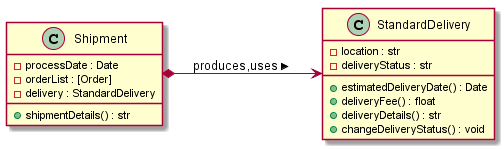
\includegraphics[keepaspectratio]{https://raw.githubusercontent.com/HowDoIGitHelp/CMSC23MDNotes/master/Markdown\%20Lecture\%20Notes\%20and\%20Lab\%20Exercises/uml/nonfactorymethodExample.png}}
\caption{online marketplace}
\end{figure}

This system does work. It works but it is still inelegant. As soon as
your app grows, you will incorporate new delivery options like express
delivery, or pickups or whatever. Every time you need to add a new
delivery method you will need to perform surgery in \texttt{Shipment}
since the \texttt{StandardDelivery} instance is created inside the
constructor of \texttt{Shipment}. \texttt{Shipment}'s code is too
coupled with \texttt{StandardDelivery}.

To solve this you need to implement the factory method pattern. Right
now shipment is a factory since it constructs its own instance of
\texttt{StandardDelivery}. To refactor this into elegant code, you need
to so create an abstraction called\texttt{Delivery} first to support
polymorphism. Inside \texttt{Shipment} instead of creating instances of
\texttt{Delivery}'s using a constructor, you invoke a factory method
that encapsulates the instantiation of \texttt{Delivery}. In this case
we name this method \texttt{newDelivery()}. All it does is return an
instance of \texttt{StandardDelivery} using its constructor.

\begin{figure}
\centering
\pandocbounded{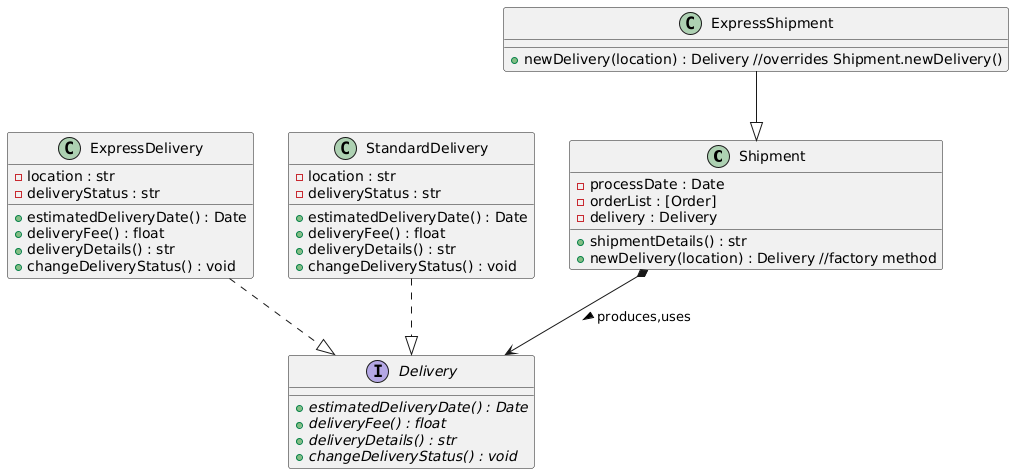
\includegraphics[keepaspectratio]{https://raw.githubusercontent.com/HowDoIGitHelp/CMSC23MDNotes/master/Markdown\%20Lecture\%20Notes\%20and\%20Lab\%20Exercises/uml/factorymethodExample.png}}
\caption{online marketplace}
\end{figure}

In this new architecture, whenever there are new delivery methods a
shipment could have, all you have to do is to create a realization of
that delivery method. In this case the new delivery method is
\texttt{ExpressDelivery} which delivers for two days but is twice as
expensive. And instead of changing \texttt{Shipment} (violates
Open/Closed Principle), you make an extension to \texttt{Shipment}. This
extension is the specialization to shipment called
\texttt{ExpressShipment} (a shipment that uses express delivery). In
this specialization, you only need to override the factory method
delivery, so that every instance of delivery construction creates
\texttt{ExpressDelivery}. The difference between
\texttt{ExpressDelivery} and \texttt{Delivery} is that
\texttt{ExpressDelivery} has a delivery fee of 1000 and the estimated
delivery date is 1 day after the processing date.

\subsection{Why this is
elegant}\label{creational-patterns.md__why-this-is-elegant}

\begin{itemize}
\tightlist
\item
  \textbf{Single Responsibility Principle} - the extra level of
  encapsulation on the construction of the product (factory method),
  allows the factory to be responsible of creating the exact product
  type it needs.
\item
  \textbf{Open/Closed Principle} - instead of modifying the factory to
  incorporate the creation of different product realizations, you
  instead create an extension of the factory. No need for introspective
  checks since the factory method supports polymorphism of the product
  it creates.
\item
  \emph{Encapsulate what varies} - This pattern upholds one of OOP
  paradigms most important principles. Since the construction of product
  varies from product type to product type, it is encapsulated into the
  factory method.

  \begin{itemize}
  \tightlist
  \item
    This avoids tight \textbf{coupling} between the factory and the
    product
  \end{itemize}
\end{itemize}

\begin{quote}
Coupled classes are classes which are very dependent on each other.
Changing the code of one will most likely affect the other
\end{quote}

\subsection{How to implement
it:}\label{creational-patterns.md__how-to-implement-it}

\begin{enumerate}
\def\labelenumi{\arabic{enumi}.}
\tightlist
\item
  Create an abstraction for all product types (\texttt{Product}).
\item
  Inside the base factory create the the factory method function
  \texttt{newProduct():Product}. Make sure it is specified to return
  abstraction \texttt{Product}.\\
\item
  For every new product type that is added to the system, create 2 new
  classes: the new product type as a realization of \texttt{Product}
  and, and the factory for the new product type as a realization of
  \texttt{Factory}.
\item
  Inside each factory specialization override \texttt{newProduct()} to
  return the correct realization of \texttt{Product}.
\item
  Replace every instance of constructor calls inside \texttt{Factory}
  with a call to the factory method \texttt{newProduct()}.
\end{enumerate}

\section{Abstract
Factory}\label{creational-patterns.md__abstract-factory}

\subsection{Problem}\label{creational-patterns.md__problem-1}

Your system consists of a family of related products. These products
also have different variants. You need a way to create these products so
that the products match the the same variant. The exact variants of the
family of products are decided during runtime, somewhere else in the
code (similar to product creation in a factory method)

\begin{figure}
\centering
\pandocbounded{\includegraphics[keepaspectratio]{https://raw.githubusercontent.com/HowDoIGitHelp/CMSC23MDNotes/master/Markdown\%20Lecture\%20Notes\%20and\%20Lab\%20Exercises/copyright\%20free\%20drawings/Abstract\%20Factory.png}}
\caption{Abstract Factory}
\end{figure}

\subsection{Solution}\label{creational-patterns.md__solution-1}

You create different kinds of factories that realize under the same
abstract factory. The exact type of factory will decide the variant of
the family of products that are created. To do this you need to create
different factory methods for each product. These factory methods must
be abstract methods in the abstract factory so that every factory
realization can create all members of the product family.

\begin{figure}
\centering
\pandocbounded{\includesvg[keepaspectratio]{https://raw.githubusercontent.com/HowDoIGitHelp/CMSC23MDNotes/master/Markdown\%20Lecture\%20Notes\%20and\%20Lab\%20Exercises/uml/abstractFactory.svg}}
\caption{abstract factory}
\end{figure}

The family of products, are \texttt{ProductA} and \texttt{ProductB},
These products come in two variants, variant 1 and 2.
\texttt{FactoryVariant1} is a realization of \texttt{Factory} which
creates all of the product in variant 1 while \texttt{FactoryVariant2}
creates all the products in variant 2.

\begin{quote}
If it makes sense for the system, you can make an abstract
\texttt{Product} class for all the types of products.
\end{quote}

When the client of an abstract factory produces its products, it doesn't
need to know what kind of factory is producing the products. This means
that the concrete type of a product (its variant) is not decided during
compile time but instead it depends on the concrete type of the factory
that is creating it.

\subsection{Example}\label{creational-patterns.md__example-1}

\subsubsection{Bootleg Text-based Zelda
Game}\label{creational-patterns.md__bootleg-text-based-zelda-game}

You're creating the dungeon encounter mechanics of some bootleg
text-based zelda game. In this game,every time you enter a dungeon, you
encounter 0-8 monsters (the exact number is randomly determined). There
are 3 types of monsters, bokoblins, moblins, and lizalflos (different
types have different moves). The exact type of monster is randomly
decided as well.

Right now the game works like this:

As soon as you enter the dungeon, all the enemies are announced:

\begin{verbatim}
5 monsters appeared
A lizalflos appeared
A lizalflos appeared
A lizalflos appeared
A moblin appeared
A moblin appeared
\end{verbatim}

After this, each enemy in the encounter attacks. They randomly pick an
attack from their moveset.

\begin{verbatim}
Lizalflos thorws its lizal boomerang at you for 2 damage
Lizalflos thorws its lizal boomerang at you for 2 damage
Lizalflos camouflages itself
Moblin stabs you with a spear for 3 damage
Moblin stabs you with a spear for 3 damage
\end{verbatim}

The encounter ends with Link dying since you haven't coded anything past
this part.

You decide to make things exciting for your game by adding harder
dungeons, medium dungeon and hard dungeon.

\paragraph{Medium dungeon}\label{creational-patterns.md__medium-dungeon}

Instead of encountering, normal monsters you encounter stronger versions
of the monsters, these monsters are blue colored:

\begin{itemize}
\tightlist
\item
  \textbf{Blue Bokoblin}

  \begin{itemize}
  \tightlist
  \item
    equipped with a spiked boko club and a spiked boko shield
  \item
    bludgeon deals 2 damage
  \end{itemize}
\item
  \textbf{Blue Moblin}

  \begin{itemize}
  \tightlist
  \item
    equipped with rusty halberd
  \item
    stab deals 5 damage
  \item
    kick deals 2 damage
  \end{itemize}
\item
  \textbf{Blue Lizalflos}

  \begin{itemize}
  \tightlist
  \item
    equipped with a forked boomerang
  \item
    throw boomerang deals 3 damage
  \end{itemize}
\end{itemize}

\paragraph{Hard dungeon}\label{creational-patterns.md__hard-dungeon}

These monsters are silver colored extra stronger versions of the
monsters

\begin{itemize}
\tightlist
\item
  \textbf{Silver Bokoblin}

  \begin{itemize}
  \tightlist
  \item
    equipped with a dragonbone boko club and a dragonbone boko shield
  \item
    bludgeon deals 5 damage
  \end{itemize}
\item
  \textbf{Silver Moblin}

  \begin{itemize}
  \tightlist
  \item
    equipped with knight's halberd
  \item
    stab deals 10 damage
  \item
    kick deals 3 damage
  \end{itemize}
\item
  \textbf{Silver Lizalflos}

  \begin{itemize}
  \tightlist
  \item
    equipped with a tri-boomerang
  \item
    throw boomerang deals 7 damage
  \end{itemize}
\end{itemize}

To seamlessly incorporate these harder monsters in your system, you need
to create an abstract factory for each dungeon difficulty. There are now
three variants for each monster. For every variant, there is a factory
that spawns new instances of each monster.

\begin{figure}
\centering
\pandocbounded{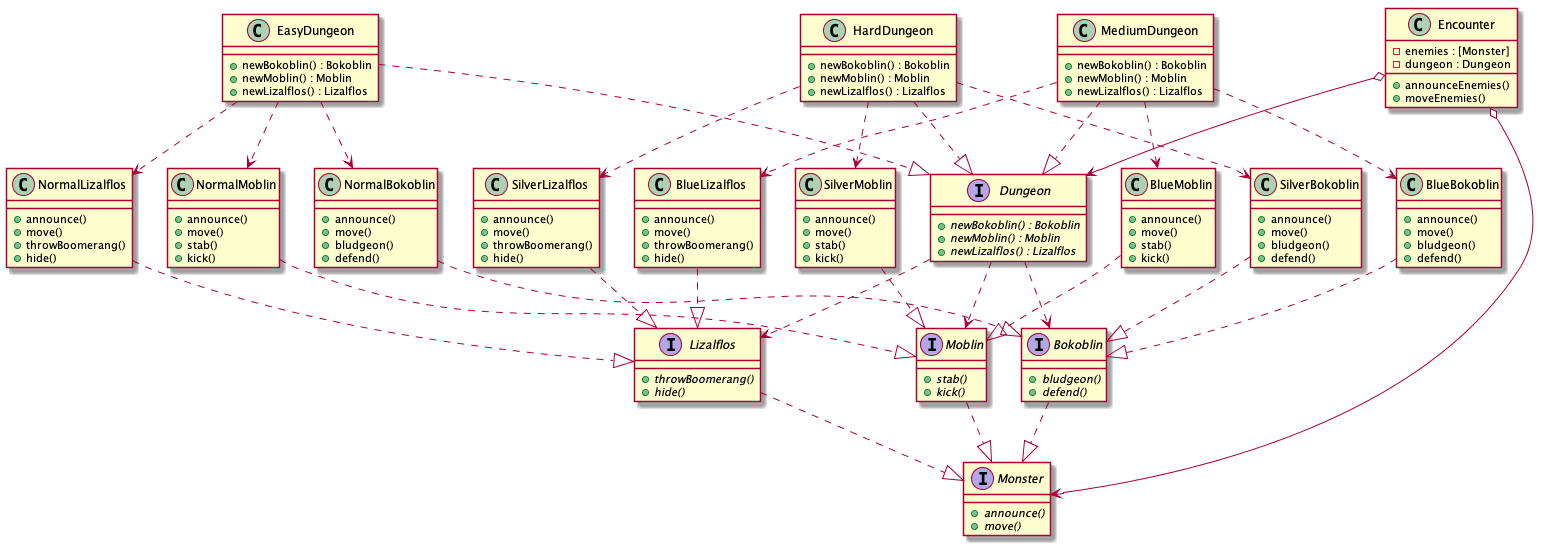
\includegraphics[keepaspectratio]{https://raw.githubusercontent.com/HowDoIGitHelp/CMSC23MDNotes/master/Markdown\%20Lecture\%20Notes\%20and\%20Lab\%20Exercises/uml/abstractFactoryExample.png}}
\caption{abstract factory example}
\end{figure}

\subsection{Why this is
elegant}\label{creational-patterns.md__why-this-is-elegant-1}

\begin{itemize}
\tightlist
\item
  \textbf{Open/Closed Principle} - This solution is easier to maintain
  since you can add more variants of \texttt{Product} without touching
  any existing code. All you have to do is to add new realization for
  \texttt{Product} and a new realization \texttt{AbstractFactory}
\item
  Changing the form and behavior of specific variants are isolated since
  its creation is abstracted.
\item
  You can easily switch between variants by swapping out the factory.
\end{itemize}

\subsection{How to implement
it:}\label{creational-patterns.md__how-to-implement-it-1}

\begin{itemize}
\tightlist
\item
  For every product in the family of products, create an abstraction of
  it (\texttt{ProductA}, \texttt{ProductB}).
\item
  For every variant of the products, create a factory,
  (\texttt{FactoryVariant1}, \texttt{FactoryVariant2}). These factories
  must realize under an abstract \texttt{AbstractFactory}. The factory
  should contain abstract factory methods for each product,
\item
  Inside every factory realization implement all factory methods.
\end{itemize}

\section{Singleton Pattern (Optional
Read)}\label{creational-patterns.md__singleton-pattern-optional-read}

\subsection{Problem}\label{creational-patterns.md__problem-2}

Sometimes it wouldn't make sense for a class to have more than one
instance in the lifetime of the application. These things are called
singletons.

\subsection{Solution}\label{creational-patterns.md__solution-2}

Inside the singleton. Create a static attribute that represents the
singleton. Since it is static all instances of the class will share this
value. Create a builder to lazily instantiate the value of the singleton
and expose the value of the instance.

Disallow the usage of the normal constructor as much as possible. To
access the shared static instance, use the builder.

\begin{figure}
\centering
\pandocbounded{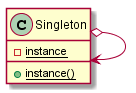
\includegraphics[keepaspectratio]{https://raw.githubusercontent.com/HowDoIGitHelp/CMSC23MDNotes/master/Markdown\%20Lecture\%20Notes\%20and\%20Lab\%20Exercises/uml/singleton.png}}
\caption{singleton}
\end{figure}

\begin{quote}
Disallowing the creation of a singleton depends on the language you use,
you can set the constructor to private, or you can raise an error if you
try to use the constructor outside the instance builder.

You can also choose to not disallow the use of the constructor, as long
as you trust the users to always use the instance builder instead.
\end{quote}

\subsection{Example}\label{creational-patterns.md__example-2}

\subsubsection{A Catalog of
Globals}\label{creational-patterns.md__a-catalog-of-globals}

It doesn't make sense for you to keep multiple copies of global
variables in your application, so you decide to place them in a
singleton class.

\subsubsection{Why this is NOT
elegant}\label{creational-patterns.md__why-this-is-not-elegant}

A singleton pattern is actually hated by most developers. Yes you can
ensure that there is exactly one instance of a class, but its advantages
come with a lot of drawbacks.

\begin{itemize}
\tightlist
\item
  You can ensure single instance classes, just by being vigilant.
\item
  Singletons require the use of static attributes and methods. Statics
  are anti-pattern because they are global variables and manipulators
  that can have invisible changes to state.
\item
  Singletons are usually symptoms of bad design.
\end{itemize}

\section{Optional
Reading}\label{creational-patterns.md__optional-reading}

Shvets A. (2018)
\href{https://sourcemaking.com/design_patterns/creational_patterns}{Creational
Patterns} Accessed August 31, 2020

\chapter{Behavioral
Patterns}\label{behavioral-patterns.md__behavioral-patterns}

\section{Introduction}\label{behavioral-patterns.md__introduction}

Some systems require complex and extremely decoupled relationships.
Behavioral patterns are used on these tightly interconnected systems so
that they are easier to maintain. These patterns separate behavioral
responsibilities among the classes in your system in such a way that
volatile behaviors are encapsulated deep into your object structure.

\section{Learning
Outcomes}\label{behavioral-patterns.md__learning-outcomes}

\begin{enumerate}
\def\labelenumi{\arabic{enumi}.}
\tightlist
\item
  Design systems that apply the strategy pattern
\item
  Design systems that apply the state pattern
\item
  Design systems that apply the command pattern
\item
  Design systems that apply the observer pattern
\item
  Design systems that apply the template pattern
\item
  Design systems that apply the iterator pattern
\end{enumerate}

\begin{center}\rule{0.5\linewidth}{0.5pt}\end{center}

\section{Strategy
pattern}\label{behavioral-patterns.md__strategy-pattern}

\subsection{Problem}\label{behavioral-patterns.md__problem}

Some systems require behavior that have to be parametrized for other
behavior. This is easily done in a functional programming environment
since higher order functions are used to represent these. In programming
languages that don't support these features, the strategy pattern is
used.

\begin{figure}
\centering
\pandocbounded{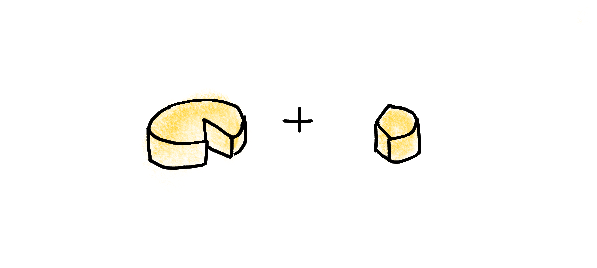
\includegraphics[keepaspectratio]{https://raw.githubusercontent.com/HowDoIGitHelp/CMSC23MDNotes/master/Markdown\%20Lecture\%20Notes\%20and\%20Lab\%20Exercises/copyright\%20free\%20drawings/Strategy.png}}
\caption{strategy}
\end{figure}

\subsection{Solution}\label{behavioral-patterns.md__solution}

Functions that are not first class citizens are encapsulated inside a
\texttt{Strategy} class. A strategy class simply contains the method
\texttt{execute(params)}, which represents the behavior that should be
passed into a higher order function. Any method that can be passed into
the higher order function should realize \texttt{Strategy}.

\begin{figure}
\centering
\pandocbounded{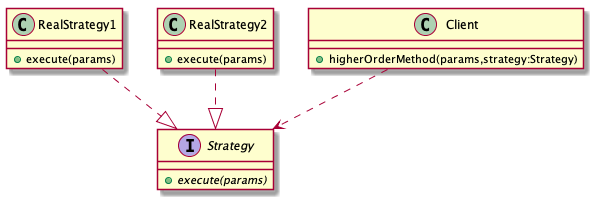
\includegraphics[keepaspectratio]{https://raw.githubusercontent.com/HowDoIGitHelp/CMSC23MDNotes/master/Markdown\%20Lecture\%20Notes\%20and\%20Lab\%20Exercises/uml/strategy.png}}
\caption{Strategy pattern}
\end{figure}

The object \texttt{params} represent the data that you need to pass into
the correct class. In this pattern you pass the the whole
\texttt{Strategy} realization so that \texttt{strategy.execute(params)}
perform the desired behavior. You can add other methods in the
\texttt{Strategy} abstraction, if it makes sense for the system.

\subsection{Example}\label{behavioral-patterns.md__example}

\subsubsection{Fraction
Calculations}\label{behavioral-patterns.md__fraction-calculations}

You're creating a less sophisticated version of a fraction calculator.
This calculator only has arithmetic operations inside it, addition,
subtraction, division, and multiplication. Inside this calculator, a
calculation is represented in a \texttt{Calculation} instance. Every
calculation has four parts:

\begin{itemize}
\tightlist
\item
  \texttt{\_\_left} - represents the left operand fraction
\item
  \texttt{\_\_right} - represents the right operand fraction
\item
  \texttt{\_\_operation} - represents the operation
  (\(+\),\(-\),\(\times\),\(\div\))
\item
  \texttt{\_\_answer} - represents the solution of the calculation
\end{itemize}

Python does indeed support higher order functions but your boss is
anti-functional programming so he forbids the use these features.
Because of this you decide to implement the strategy pattern.

To do this, you need to create an abstraction called \texttt{Operation}
to represent the different operations. For each operation, you create a
class that realizes \texttt{Operation}.

\begin{figure}
\centering
\pandocbounded{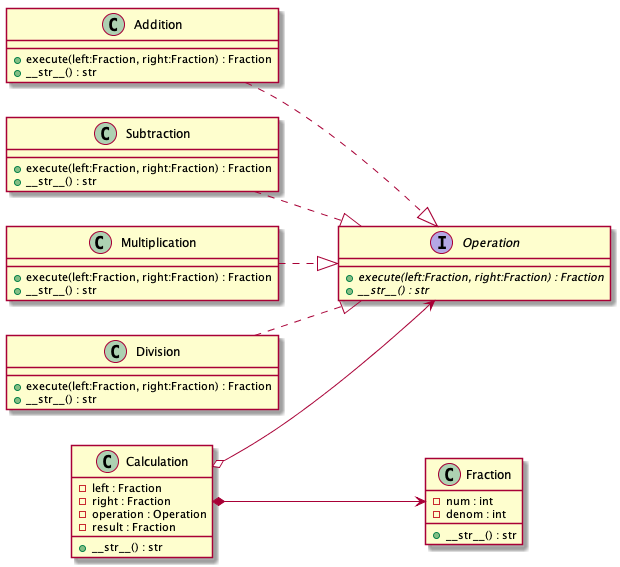
\includegraphics[keepaspectratio]{https://raw.githubusercontent.com/HowDoIGitHelp/CMSC23MDNotes/master/Markdown\%20Lecture\%20Notes\%20and\%20Lab\%20Exercises/uml/strategyexample.png}}
\caption{strategy pattern example}
\end{figure}

\begin{quote}
\texttt{execute()} should have been named like a builder method
(something like \texttt{solution()}), I'm keeping the name
\texttt{execute()} since this is how Strategy patterns usually names
this particular method.
\end{quote}

\subsection{Why this is
elegant}\label{behavioral-patterns.md__why-this-is-elegant}

\begin{itemize}
\tightlist
\item
  \textbf{Open/Closed Principle} - If you want to add new strategies,
  you wouldn't need to touch any existing code.
\item
  The implementation of a strategy is deeply tucked inside multiple
  layers of encapsulation. Changing these implementations is very easy.
\item
  You can swap strategies during runtime in the same way you do in
  functional programming.
\end{itemize}

\subsection{How to implement
it}\label{behavioral-patterns.md__how-to-implement-it}

\begin{enumerate}
\def\labelenumi{\arabic{enumi}.}
\tightlist
\item
  Create an abstract \texttt{Strategy} that contains an abstract method
  called \texttt{execute}. This method should be specified to accept all
  the necessary parameters needed by your parameterized function.
\item
  For every strategy, the higher order method can accept, you create a
  realization for \texttt{Strategy} and implement the correct behavior
  in \texttt{execute}.
\item
  The higher order function should now be specified to accept a
  \texttt{strategy} of type \texttt{Strategy}.
\item
  Inside the higher order function, whenever it wants to perform the
  strategies embedded behavior, call \texttt{strategy.execute(...)}.
\end{enumerate}

\section{State Pattern}\label{behavioral-patterns.md__state-pattern}

\subsection{Problem}\label{behavioral-patterns.md__problem-1}

Some objects can change into many different states. If different objects
behavior is dependent on its current state, it would require, bulky and
annoying if-else blocks to handle its dynamic behavior.

\begin{figure}
\centering
\pandocbounded{
\includegraphics[keepaspectratio]{https://raw.githubusercontent.com/HowDoIGitHelp/CMSC23MDNotes/master/Markdown\%20Lecture\%20Notes\%20and\%20Lab\%20Exercises/copyright\%20free\%20drawings/State.png}}
\caption{State}
\end{figure}

\subsection{Solution}\label{behavioral-patterns.md__solution-1}

An object that can have many states should contain an attribute
representing its state. Instead of performing, state dependent behavior
directly inside the object, you delegate this responsibility to its
embedded state instead. In this way the object will behave according to
its current state.

\begin{figure}
\centering
\pandocbounded{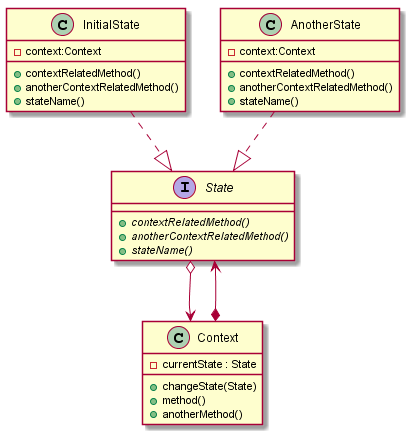
\includegraphics[keepaspectratio]{https://raw.githubusercontent.com/HowDoIGitHelp/CMSC23MDNotes/master/Markdown\%20Lecture\%20Notes\%20and\%20Lab\%20Exercises/uml/state.png}}
\caption{state pattern}
\end{figure}

The state may be required to contain backreference to the context object
that owns it. This is only required if state methods requires to
access/control the context that owns it.

\begin{figure}
\centering
\pandocbounded{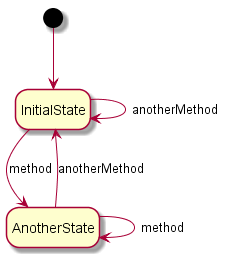
\includegraphics[keepaspectratio]{https://raw.githubusercontent.com/HowDoIGitHelp/CMSC23MDNotes/master/Markdown\%20Lecture\%20Notes\%20and\%20Lab\%20Exercises/uml/statediagram.png}}
\caption{state diagram}
\end{figure}

\subsection{Example}\label{behavioral-patterns.md__example-1}

\subsubsection{States of
matter}\label{behavioral-patterns.md__states-of-matter}

The state of any given matter is dependent on the pressure and
temperature of its environment. If you heat up some liquid enough it
will turn to gas, if you compress it enough it will become solid.

You are to build a less sophisticated version of this model in code.
Matter comes in three states, solid, liquid, and gas. The state of the
matter may change if you put/remove pressure on it or heat/cool it.

The state diagram would look something like this:

\begin{figure}
\centering
\pandocbounded{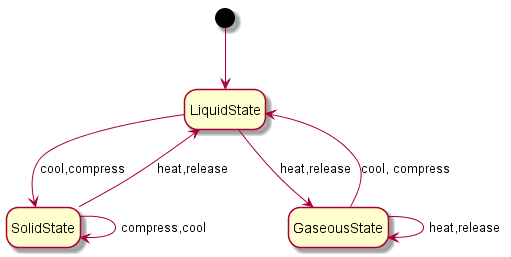
\includegraphics[keepaspectratio]{https://raw.githubusercontent.com/HowDoIGitHelp/CMSC23MDNotes/master/Markdown\%20Lecture\%20Notes\%20and\%20Lab\%20Exercises/uml/statediagramexample.png}}
\caption{state diagram example}
\end{figure}

To implement something like this, you would need to create matter which
owns an attribute called \texttt{state} which represents the matter's
current state. Since there are three states, you create three
realizations to a common abstraction to state.

When you compress/release/cool/heat the matter, you delegate the
appropriate behavior and state change inside \texttt{state}'s version of
that. Each \texttt{State} realization will need a backreference to the
\texttt{Matter} that owns it so that it can change it's state.

\begin{quote}
Delegating behavior to the composed state means that, when the
\texttt{Matter} instances invoke, \texttt{compress()},
\texttt{relaease()} \texttt{heat()}, and \texttt{cool()}, the composed
\texttt{State} owned by the matter calls its own version of
\texttt{compress()}, \texttt{relaease()} \texttt{heat()}, and
\texttt{cool()}.
\end{quote}

\begin{figure}
\centering
\pandocbounded{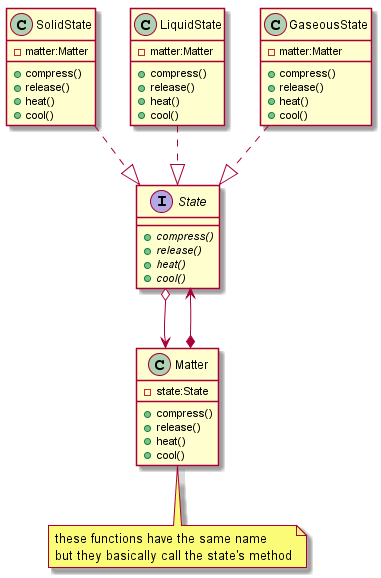
\includegraphics[keepaspectratio]{https://raw.githubusercontent.com/HowDoIGitHelp/CMSC23MDNotes/master/Markdown\%20Lecture\%20Notes\%20and\%20Lab\%20Exercises/uml/stateexample.png}}
\caption{state example}
\end{figure}

\begin{quote}
Matter owns an instance of \texttt{State}, and that instance has an
attribute called \texttt{matter}. The attribute \texttt{matter} is the
reference to the instance of \texttt{Matter} that owns it. The
\texttt{State} instance needs this reference so that it can change the
matter's state when it is compressed, released, heated, or cooled.
\end{quote}

\subsection{Why this is
elegant}\label{behavioral-patterns.md__why-this-is-elegant-1}

\begin{itemize}
\tightlist
\item
  \textbf{Single Responsibility Principle} - behavior related to state
  is delegated to the state itself.
\item
  \textbf{Open/Closed Principle} - You can incorporate new states to the
  system without touching any existing client code
\item
  Implementing this pattern will remove bulky and annoying state
  conditionals
\end{itemize}

\subsection{How to implement
it}\label{behavioral-patterns.md__how-to-implement-it-1}

\begin{enumerate}
\def\labelenumi{\arabic{enumi}.}
\tightlist
\item
  Create an abstract \texttt{State} that contains abstract methods for
  all state dependent behavior (context related behaviors that are
  dependent on context's state).
\item
  For every state the \texttt{Context} can have, create a realization of
  \texttt{State}.
\item
  \texttt{Context} owns an attribute that represents the current state
  (\texttt{currentState}) that it owns.
\item
  If the state needs to control the \texttt{Context} instance that owns
  it, add a backreference to \texttt{Context} inside state.
\item
  Whenever a \texttt{Context} instance performs state dependent methods,
  it calls \texttt{currentState.contextRelatedMethod()} instead so that
  its behavior is dependent on its current state.
\end{enumerate}

\section{Command Pattern}\label{behavioral-patterns.md__command-pattern}

\subsection{Problem}\label{behavioral-patterns.md__problem-2}

Sometimes, object behavior contain complicated constraints. Sometimes,
the system require the behavior to be invoked by an object but performed
by another (this is common in presentation layer/domain layer separation
in MVC enterprise systems). Sometimes, the system requires behavior to
be undone. Sometimes the system requires a history of the behaviors that
were being performed.

\begin{figure}
\centering
\pandocbounded{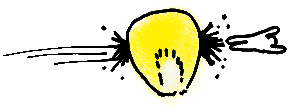
\includegraphics[keepaspectratio]{https://raw.githubusercontent.com/HowDoIGitHelp/CMSC23MDNotes/master/Markdown\%20Lecture\%20Notes\%20and\%20Lab\%20Exercises/copyright\%20free\%20drawings/Command.png}}
\caption{Command (What does this strange picture mean?)}
\end{figure}

\subsection{Solution}\label{behavioral-patterns.md__solution-2}

These problems have a common solution, the \textbf{command pattern}. A
\texttt{Command} is a more powerful version of a \texttt{Strategy}.
While both of them encapsulates behavior, a \texttt{Strategy} is just
that, a function wrapper. A \texttt{Command} on the other hand contains
which object performs the behavior, which parameters are needed to
perform the behavior, and how to undo the command (if needed).

Creating \texttt{Command}s, allow for more flexible behavior
responsibility assignments. A separate \texttt{Invoker} object triggers
the behavior by creating a command. This \texttt{Invoker} prepares the
command with the appropriate \texttt{Reciever} (the object performing
the command), and the appropriate parameters. The invoker then executes
the prepared command. The command doesn't actually do anything, it just
tells the \texttt{Reciever} to call the appropriate method.

This separation of responsibility allows for the creation of extra
features that may be required for your system:

\begin{itemize}
\item
  If you want to keep a history of the performed commands, the
  \texttt{Invoker} may keep a list of \texttt{Commands}. This way the
  data stored in the list history, is a perfect representation of the
  previous commands.
\item
  If you want the \texttt{Commands} to be undoable, you can store a
  backup of the receiver (and other affected objects) by the
  \texttt{Command} inside each instance of \texttt{Command} . Undoing a
  command will be as simple as restoring the receiver to its backup.
\end{itemize}

\begin{figure}
\centering
\pandocbounded{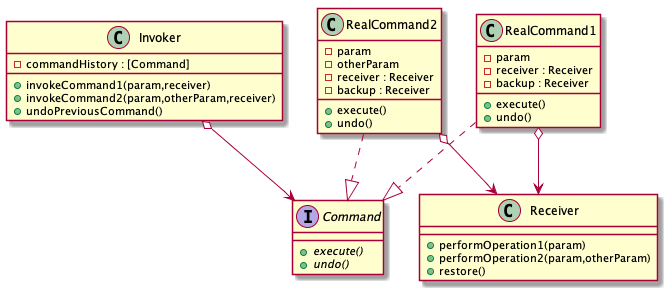
\includegraphics[keepaspectratio]{https://raw.githubusercontent.com/HowDoIGitHelp/CMSC23MDNotes/master/Markdown\%20Lecture\%20Notes\%20and\%20Lab\%20Exercises/uml/command.png}}
\caption{command pattern}
\end{figure}

\begin{quote}
Instead of passing the receiver in the \texttt{Invoker} methods, you can
create an attribute called receiver inside \texttt{Invoker}. But doing
this will make it so there is one \texttt{Receiver} instance for every
\texttt{Invoker} instance.

The commands should only affect the receiver. If the behavior that is
performed changes a lot of objects, then make a \texttt{Receiver} class
that encapsulates all of the affected objects. Doing this will make the
implementation of undo easier since the backup inside of the command
will simply be an older version of \texttt{Receiver}.

Different command realizations are not necessarily of the
same\texttt{Strategy}. That's why the parameters of the behavior are
stored as attributes of the command, not passed in the
\texttt{execute()} function. This is so that no matter what the command
is, all \texttt{execute()} functions will have the same type signatures.
\end{quote}

\subsection{Example}\label{behavioral-patterns.md__example-2}

\subsubsection{Zooming through a
maze}\label{behavioral-patterns.md__zooming-through-a-maze}

You're creating a maze navigation game thing. This is what the
application currently has right now:

\begin{itemize}
\tightlist
\item
  \texttt{Board} - this represents the layout of the maze. The layout is
  loaded from a file. It has these attributes:

  \begin{itemize}
  \tightlist
  \item
    \texttt{\_\_isSolid} - this is a 2 dimensional grid encoded as a
    nested list of booleans which represents the solid boundaries of the
    maze. For example if \texttt{\_\_isSolid{[}row{]}{[}col{]}} is true
    then it means that that cell on (row,col) is a boundary
  \item
    \texttt{\_\_start} - a tuple of two integers that represent where
    the character starts
  \item
    \texttt{\_\_end} - tuple of two integers that represent the position
    of the end of the maze
  \item
    \texttt{\_\_cLoc} - tuple of two integers that represents the
    current location of the character
  \item
    \texttt{moveUp()}, \texttt{moveDown()}, \texttt{moveLeft()},
    \texttt{moveRight()} - moves the character one space, in the
    respective direction. The character cannot move to a boundary cell,
    it will raise an error instead.
  \item
    \texttt{canMoveUp()}, \texttt{canMoveDown()},
    \texttt{canMoveLeft()}, \texttt{canMoveRight()} - returns true if
    the cell in the respective direction is not solid.
  \item
    \texttt{\_\_str()\_\_} string representation of the board. It shows
    which are the boundaries and the character location
  \end{itemize}
\end{itemize}

What's missing right now is controller support. This is how a player
controls the character on the maze:

\begin{itemize}
\tightlist
\item
  \texttt{dpad\_up()}, \texttt{dpad\_down()}, \texttt{dpad\_left()},
  \texttt{dpad\_right()} - The character dashes through the maze in the
  specified direction until it hits a boundary.
\item
  \texttt{a\_button()} - The character undoes the previous action it
  did.
\end{itemize}

To implement controller support you need to create a \texttt{Command}
abstraction which is realized by all controller commands. The
\texttt{Controller} (which represents the controller) is the invoker for
the commands. Since commands are undoable, this controller needs to keep
a command history, represented as a list. Every time a controller button
is pressed, it creates the appropriate \texttt{Command}, executes it and
appends it to the command history. Every time the \texttt{a\_button()}
is pressed to undo, the controller pops the last command from the
command history and undoes it.

\begin{figure}
\centering
\pandocbounded{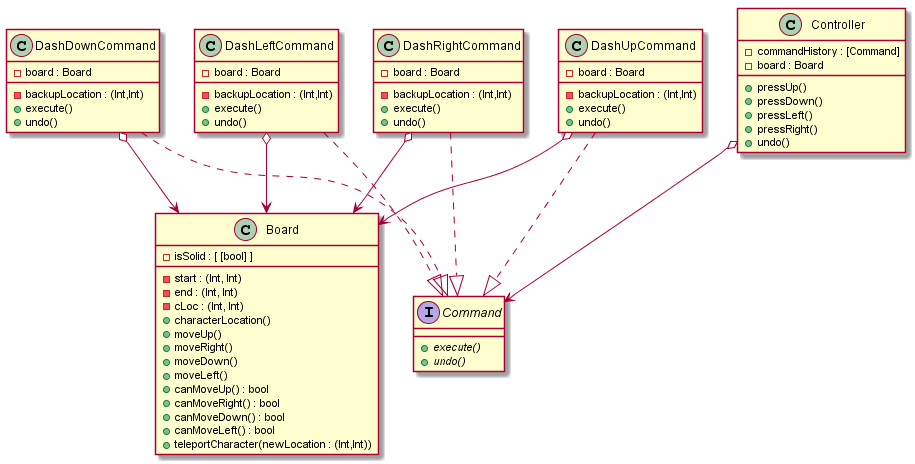
\includegraphics[keepaspectratio]{https://raw.githubusercontent.com/HowDoIGitHelp/CMSC23MDNotes/master/Markdown\%20Lecture\%20Notes\%20and\%20Lab\%20Exercises/uml/commandexample.png}}
\caption{command example}
\end{figure}

\subsection{Why this is
elegant}\label{behavioral-patterns.md__why-this-is-elegant-2}

\begin{itemize}
\tightlist
\item
  \textbf{Single Responsibility Principle} - The behavioral
  responsibilities in the system are thoroughly separated. One invokes
  the command, and the other performs the behavior associated with the
  command.
\item
  \textbf{Open/Closed Principle} - If there are more commands you want
  to add, you don't have to touch any existing code.
\item
  Switching between invokers and receivers is easily done
\item
  You can implement undo (and redo)
\item
  You can defer the execution of behavior
\item
  A command may be made of smaller simpler commands
\end{itemize}

\subsection{How to implement
it}\label{behavioral-patterns.md__how-to-implement-it-2}

\begin{enumerate}
\def\labelenumi{\arabic{enumi}.}
\tightlist
\item
  Create an abstraction \texttt{Command} that contains abstract method
  \texttt{execute()}, and other command related methods like
  \texttt{undo()}.
\item
  For every command, create a realization to \texttt{Command}. These
  commands uses a reference to a \texttt{Reciever} instance. This
  instance represents the instance/s that are affected whenever
  \texttt{Command} realizations are executed.
\item
  Create an \texttt{Invoker} class that will be responsible for
  instantiating, preparing, and executing commands. Inside these class
  are methods for invoking each commands. When these methods are called,
  the invoker does the following:

  \begin{enumerate}
  \def\labelenumii{\arabic{enumii}.}
  \tightlist
  \item
    Instantiate an instance of \texttt{Command} called \texttt{c} with
    the correct realization.
  \item
    select the receiver of the \texttt{Command}, including the related
    parameters.
  \item
    invoke \texttt{c.execute()}.
  \end{enumerate}
\item
  If the system supports undoable commands, the \texttt{Invoker} should
  keep a list of commands called \texttt{commandHistory} and each
  command instance should keep a reference called \texttt{backup} to
  enable restoration of \texttt{Reciever} instances.
\end{enumerate}

\section{Observer
Pattern}\label{behavioral-patterns.md__observer-pattern}

\subsection{Problem}\label{behavioral-patterns.md__problem-3}

What if you need to inform a lot of objects about the changes to some
interesting data? If you globalize the data and let your client objects
poll for changes all the time, this will affect the security and safety
of your interesting data. Plus, global data is something that should be
avoided as much as possible. Also, forcing your objects poll for changes
all the time will be inefficient if your interesting data has not
changed.

\begin{figure}
\centering
\pandocbounded{
\includegraphics[keepaspectratio]{https://raw.githubusercontent.com/HowDoIGitHelp/CMSC23MDNotes/master/Markdown\%20Lecture\%20Notes\%20and\%20Lab\%20Exercises/copyright\%20free\%20drawings/Observer.png}}
\caption{observer}
\end{figure}

\subsection{Solution}\label{behavioral-patterns.md__solution-3}

The responsibility of sharing information about the changes to
interesting data should not be placed in the clients of the data. You
should create a notifier class that encapsulates the interesting data.
This class should be responsible of notifying interested clients about
changes on the data.

To do this you need to encapsulate the interesting data (from now on
lets call it the \texttt{subject}), into a \texttt{Publisher} class. An
instance of this class will be responsible of notifying the observers
for any change in the \texttt{subject}. Whenever there are changes to
the subject, the \texttt{Publisher} instance calls
\texttt{notifyObservers()} so that all interested, observers will be
informed of the change. Any class that is potentially interested in the
\texttt{subject} should realize an \texttt{Observer} abstraction, which
in the bare minimum contains, the \texttt{update(updatedSubject)}
function. Inside \texttt{Publisher}'s \texttt{notifyObservers()} method,
every subscriber (an interested observer) is updated
(\texttt{subscriber.update()}).

Any instance of an \texttt{Observer} should be subscribed to the change
notifications using \texttt{Publisher}'s \texttt{subscribe()} function.
They can also be unsubscribed using the\texttt{unsubscribe()} function.

\begin{figure}
\centering
\pandocbounded{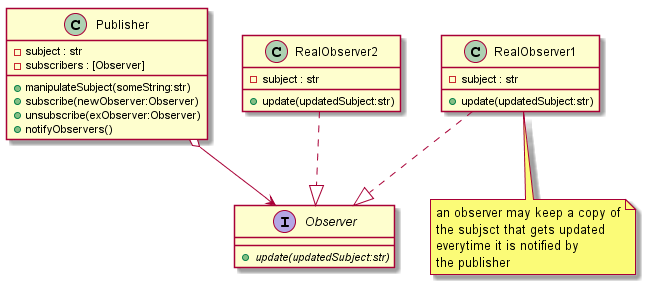
\includegraphics[keepaspectratio]{https://raw.githubusercontent.com/HowDoIGitHelp/CMSC23MDNotes/master/Markdown\%20Lecture\%20Notes\%20and\%20Lab\%20Exercises/uml/observer.png}}
\caption{observer}
\end{figure}

\begin{quote}
Whenever an observer has updated, the publisher needs to pass all the
necessary details in the notification. This is generally done by passing
the updated subject in the \texttt{update(updatedSubject)} method.

In some cases, the observer needs to keep a copy of the subject as an
attribute. Make sure to change the value of this attribute during
updates.

Make sure that changes to the subject are only done using the
\texttt{Publisher} class (\texttt{manipulateSubject()}). If you change
the subject without using \texttt{Publisher}'s methods, your subscribers
won't be notified.
\end{quote}

\subsection{Example}\label{behavioral-patterns.md__example-3}

\subsubsection{Push Notifier for Weather and
Headlines}\label{behavioral-patterns.md__push-notifier-for-weather-and-headlines}

You are creating a push notification system that works for multiple
platforms. You want to distribute information about the current weather
and news headlines. This system will be potentially used on many
platforms so you have to think about the maintainability issues for
adding new platform support.

To implement this, you have to apply the observer pattern. Your subject
would be \texttt{Weather} data and \texttt{Headline} data (which are
their own classes). These subjects should be encapsulated into a single
publisher class (which will be called \texttt{PushNotifier}).

Any platform, that is interested in the changes to the subject should
realize a \texttt{Subscriber} abstraction (Observer), which contains the
abstract method update().

\begin{figure}
\centering
\pandocbounded{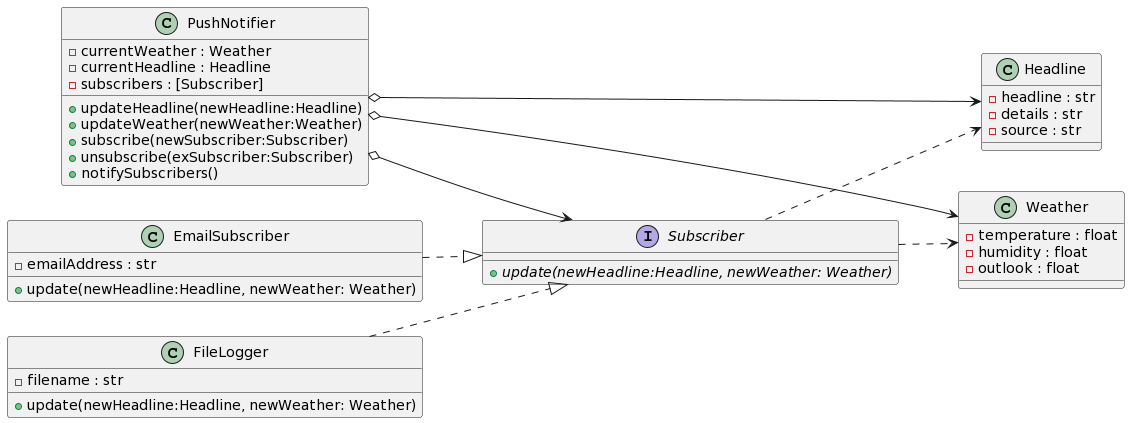
\includegraphics[keepaspectratio]{https://raw.githubusercontent.com/HowDoIGitHelp/CMSC23MDNotes/master/Markdown\%20Lecture\%20Notes\%20and\%20Lab\%20Exercises/uml/observerexample.png}}
\caption{observer example}
\end{figure}

\subsection{Why this is
elegant}\label{behavioral-patterns.md__why-this-is-elegant-3}

\begin{itemize}
\tightlist
\item
  \textbf{Open/Closed Principle} - You can add new \texttt{Observer}
  realizations seamlessly every time there are new objects that are
  interested in the subject.
\item
  A observer can be subscribed/unsubscribed during runtime
\end{itemize}

\subsection{How to implement
it}\label{behavioral-patterns.md__how-to-implement-it-3}

\begin{enumerate}
\def\labelenumi{\arabic{enumi}.}
\tightlist
\item
  Create an \texttt{Observer} abstraction that represents all classes
  that can potentially observe changes to the \texttt{Publisher}.
  \texttt{Observer} will contain the abstract method \texttt{update()}.
\item
  All classes that want to be notified about changes to the
  \texttt{subject} should realize \texttt{Observer}.
\item
  \texttt{Publisher} will either own/use an instance of the
  \texttt{subject} of interest. It will also use an attribute which is
  stores the list of \texttt{Observers} that are interested in the
  subject. To attach or detach \texttt{Observer}s, \texttt{Publisher}
  contains the methods \texttt{subscribe()} and \texttt{unsubscribe()}.
\item
  Every time \texttt{subject} is manipulated, it should be done through
  \texttt{Publisher} , because \texttt{Publisher} needs to notify all
  \texttt{Observers} in its observer list attribute after every
  manipulation. This notification is done through
  \texttt{notifyObservers()} after the end of every subject
  manipulation.
\item
  Inside the \texttt{Publisher}s \texttt{notifyObservers} method, every
  \texttt{Observer} in its list of observers invoke their
  \texttt{update()} method.
\end{enumerate}

\section{Template Method
Pattern}\label{behavioral-patterns.md__template-method-pattern}

\subsection{Problem}\label{behavioral-patterns.md__problem-4}

Say you have two or more \emph{almost} identical behaviors from
different classes. Rewriting these object behaviors as separate methods
for each class duplicates many parts of the code (especially if the
behavior has a lot of lines of code).

\begin{figure}
\centering
\pandocbounded{
\includegraphics[keepaspectratio]{https://raw.githubusercontent.com/HowDoIGitHelp/CMSC23MDNotes/master/Markdown\%20Lecture\%20Notes\%20and\%20Lab\%20Exercises/copyright\%20free\%20drawings/Template.png}}
\caption{template}
\end{figure}

\subsection{Solution}\label{behavioral-patterns.md__solution-4}

To avoid code duplication, you break down your code into individual
steps. By doing this you can create a superclass that contains the
implementation for all common steps. This superclass will also contain
the common implementation for the \textbf{template method}, the method
that combines all steps into the original object behavior. Differences
between steps will be resolved under different specializations of this
superclass.

\begin{figure}
\centering
\pandocbounded{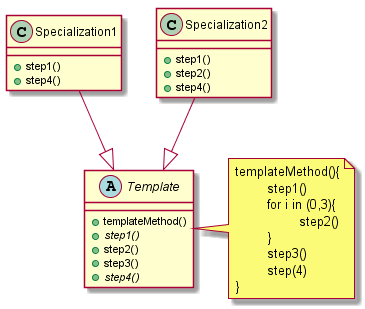
\includegraphics[keepaspectratio]{https://raw.githubusercontent.com/HowDoIGitHelp/CMSC23MDNotes/master/Markdown\%20Lecture\%20Notes\%20and\%20Lab\%20Exercises/uml/template.png}}
\caption{template method}
\end{figure}

If the exact instance of the class is a \texttt{Specialization1}, it
performs the template method with special versions of \texttt{step1()}
and \texttt{step4()} (since \texttt{Specialization1} overrides them) but
the other parts are inherited from the \texttt{Template}.

\begin{quote}
The steps in the superclass can be a mix of abstract methods and
concrete methods. Make a method abstract if you want to force all
specializations to override these steps. You'll want to do these if some
of the steps in your template doesn't have a default implementation.
\end{quote}

\subsection{Example}\label{behavioral-patterns.md__example-4}

\subsubsection{Brute Force
Recipe}\label{behavioral-patterns.md__brute-force-recipe}

If you write brute force algorithms as search problems, they will have a
common recipe. This is the reason why it is called the exhaustive search
algorithm. It will traverse all of the elements in the search space,
trying to check the validity of each element, until it completes the
solution

\textbf{Equality Search}

Search for integers equal to the target

\begin{Shaded}
\begin{Highlighting}[]
\CommentTok{\#searchSpace = [2,3,1,0,6,2,4]}
\CommentTok{\#target = 2}

\NormalTok{i }\OperatorTok{=} \DecValTok{0}
\NormalTok{solutions }\OperatorTok{=}\NormalTok{ []}
\NormalTok{candidate }\OperatorTok{=}\NormalTok{ searchSpace[}\DecValTok{0}\NormalTok{]}
\ControlFlowTok{while}\NormalTok{(i}\OperatorTok{\textless{}}\BuiltInTok{len}\NormalTok{(searchSpace)):}
    \ControlFlowTok{if}\NormalTok{ candidate }\OperatorTok{==}\NormalTok{ target:}
\NormalTok{        solutions.append(candidate)}
\NormalTok{    candidate }\OperatorTok{=}\NormalTok{ searchSpace[}\OperatorTok{++}\NormalTok{i]}
    
\CommentTok{\#solution = [2,2]}
\end{Highlighting}
\end{Shaded}

\textbf{Divisibility Search}

Search for integers divisible by the target

\begin{Shaded}
\begin{Highlighting}[]
\CommentTok{\#searchSpace = [2,3,1,0,6,2,4]}
\CommentTok{\#target = 2}

\NormalTok{i }\OperatorTok{=} \DecValTok{0}
\NormalTok{solutions }\OperatorTok{=}\NormalTok{ []}
\NormalTok{candidate }\OperatorTok{=}\NormalTok{ searchSpace[}\DecValTok{0}\NormalTok{]}
\ControlFlowTok{while}\NormalTok{(i}\OperatorTok{\textless{}}\BuiltInTok{len}\NormalTok{(searchSpace)):}
    \ControlFlowTok{if}\NormalTok{ candidate }\OperatorTok{\%}\NormalTok{ target }\OperatorTok{==} \DecValTok{0}\NormalTok{:}
\NormalTok{        solution.append(candidate)}
\NormalTok{    candidate }\OperatorTok{=}\NormalTok{ searchSpace[}\OperatorTok{++}\NormalTok{i]}
    
\CommentTok{\#solution = [2,0,6,2,4]}
\end{Highlighting}
\end{Shaded}

\textbf{Minimum Search}

No target, searches for the smallest integer

\begin{Shaded}
\begin{Highlighting}[]
\CommentTok{\#searchSpace = [2,3,1,0,6,2,4]}
\CommentTok{\#target = None}

\NormalTok{i }\OperatorTok{=} \DecValTok{1}
\NormalTok{solutions }\OperatorTok{=}\NormalTok{ [searchSpace[}\DecValTok{0}\NormalTok{]]}
\NormalTok{candidate }\OperatorTok{=}\NormalTok{ searchSpace[}\DecValTok{1}\NormalTok{]}
\ControlFlowTok{while}\NormalTok{(i}\OperatorTok{\textless{}}\BuiltInTok{len}\NormalTok{(searchSpace)):}
    \ControlFlowTok{if}\NormalTok{ candidate }\OperatorTok{\textless{}=}\NormalTok{ solutions[}\DecValTok{0}\NormalTok{]}
\NormalTok{        solutions[}\DecValTok{0}\NormalTok{] }\OperatorTok{=}\NormalTok{ candidate}
\NormalTok{    candidate }\OperatorTok{=}\NormalTok{ searchSpace[}\OperatorTok{++}\NormalTok{i]}
    
\CommentTok{\#solution = [0]}
\end{Highlighting}
\end{Shaded}

\textbf{Common Recipe}

\begin{Shaded}
\begin{Highlighting}[]
\NormalTok{i }\OperatorTok{=} \DecValTok{0}
\NormalTok{solutions }\OperatorTok{=}\NormalTok{ []}
\NormalTok{candidate }\OperatorTok{=}\NormalTok{ first()}
\ControlFlowTok{while}\NormalTok{(isStillSearching()):}
    \ControlFlowTok{if}\NormalTok{ valid(candidate):}
\NormalTok{        updateSolution(candidate)}
\NormalTok{    candidate }\OperatorTok{=} \BuiltInTok{next}\NormalTok{()}
\end{Highlighting}
\end{Shaded}

Because of this we can write a general brute force template method that
would return the solution to brute force problems. To do this you create
a superclass \texttt{SearchAlgorithm()} that contains the template
method for brute force algorithms. If you want to customize this
algorithm for special problems, all you have to do is to inherit from
\texttt{SearchAlgorithm} and override only the necessary steps.

\begin{figure}
\centering
\pandocbounded{\includesvg[keepaspectratio]{https://raw.githubusercontent.com/HowDoIGitHelp/CMSC23MDNotes/master/Markdown\%20Lecture\%20Notes\%20and\%20Lab\%20Exercises/uml/templateexample.svg}}
\caption{template example}
\end{figure}

\begin{quote}
is \texttt{isValid()} and \texttt{updateSolution(candidate)} is
different for each algorithm so it doesn't have a default
implementation. It would be best to make these steps abstract.
\end{quote}

\subsection{Why this is
elegant}\label{behavioral-patterns.md__why-this-is-elegant-4}

\begin{itemize}
\item
  \textbf{Open/Closed Principle} - The \texttt{Template} is open for
  extension but closed for modification
\item
  \emph{Encapsulate what varies} - steps can vary from specialization to
  specialization, therefore they are encapsulated into step methods.
\item
  Implementing this pattern will remove duplicate code in the common
  parts of the algorithm.
\item
  Clients may override only certain steps in a large algorithm, making
  it easier to create specializations
\end{itemize}

\subsection{How to implement
it}\label{behavioral-patterns.md__how-to-implement-it-4}

\begin{enumerate}
\def\labelenumi{\arabic{enumi}.}
\tightlist
\item
  Create an abstract class called \texttt{Template}. It contains the
  method \texttt{templateMethod()} broken down into separate steps
  through separate \texttt{step1()}, \texttt{step2()}, \ldots{} and etc.
  methods. When invoked \texttt{templateMethod()} will just call these
  step methods.
\item
  Each step method inside \texttt{Template} will contain the default
  implementation of that step. If there is no default implementation,
  the method should be abstract.
\item
  For every similar behavior to \texttt{templateMethod()} a
  specialization of \texttt{Template} is created. These methods will
  implement all abstract methods and override all step methods that vary
  for its behavior.
\end{enumerate}

\section{Iterator}\label{behavioral-patterns.md__iterator}

\subsection{Problem}\label{behavioral-patterns.md__problem-5}

One of the most common iteration recipes that you'll likely implement is
the \textbf{for-each} loop. This loop traverses a collection, and
performing some kind of operation along the way. Most programming
languages implement for each loops on built in collections like arrays,
sets, and trees. But what about non-built in collections?

\begin{figure}
\centering
\pandocbounded{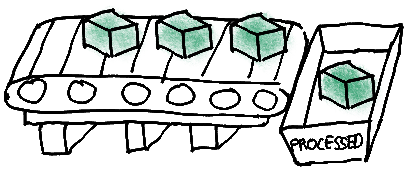
\includegraphics[keepaspectratio]{https://raw.githubusercontent.com/HowDoIGitHelp/CMSC23MDNotes/master/Markdown\%20Lecture\%20Notes\%20and\%20Lab\%20Exercises/copyright\%20free\%20drawings/Iterator.png}}
\caption{iterator}
\end{figure}

\subsection{Solution}\label{behavioral-patterns.md__solution-5}

For non built-in collections, you can create an iterator that does the
traversal for you. On the bare minimum these iterators will realize some
\texttt{Iterator} abstraction that contains the methods,
\texttt{next()}, and \texttt{hasNext()}. From these methods alone you
can easily perform complete traversals without knowing the exact type of
the collection:

\begin{Shaded}
\begin{Highlighting}[]
\NormalTok{    i }\OperatorTok{=}\NormalTok{ collection.newIterator()}
\ControlFlowTok{while}\NormalTok{ i.hasNext():}
    \BuiltInTok{print}\NormalTok{(i.}\BuiltInTok{next}\NormalTok{())}
\end{Highlighting}
\end{Shaded}

\begin{figure}
\centering
\pandocbounded{\includesvg[keepaspectratio]{https://raw.githubusercontent.com/HowDoIGitHelp/CMSC23MDNotes/master/Markdown\%20Lecture\%20Notes\%20and\%20Lab\%20Exercises/uml/iterator.svg}}
\caption{iterator}
\end{figure}

The \texttt{hasNext()} method, returns a boolean value that indicates
whether or not there are more elements to be traversed. The
\texttt{next()} method, returns the next element in the traversal.

A collection can have more than one \texttt{Iterator}s, if it makes
sense for the collection to be travsersed in more than one way. Despite
this possibility, a collection must have a default iterator which will
be the type of the new instance returned in the factory method,
\texttt{newIterator()}

\subsection{Why this is
elegant}\label{behavioral-patterns.md__why-this-is-elegant-5}

\begin{itemize}
\item
  \textbf{Single Responsibility Principle} - Traversal algorithms can
  now be placed into separate classes that interact with an iterator
  instead of the collection itself.
\item
  \textbf{Open/Closed Principle} - You can implement new types of
  collections and iterators without touching any existing code.
\item
  You can traverse all the elements in a collection, even if you don't
  know the exact type of the said collection.
\item
  Two iterators, can iterate over the same collection without problem as
  long as the iterators are of different instances.
\end{itemize}

\subsection{How to implement
it}\label{behavioral-patterns.md__how-to-implement-it-5}

\begin{enumerate}
\def\labelenumi{\arabic{enumi}.}
\tightlist
\item
  Create an abstraction called \texttt{Iterator} which contains the
  abstract methods \texttt{next()} and \texttt{hasNext()}.
\item
  Create an abstraction called \texttt{Collection} which contains the
  abstract method \texttt{newIterator()}.
\item
  For very collection that can be iterated through create a realization
  to \texttt{Collection}. Inside these \texttt{Collection} realizations,
  the \texttt{newIterator()} method must be implemented which simply
  returns a new instance of the default \texttt{Iterator}. (for
  collections that can be iterated through in more than one way, create
  different methods for creating other iterators as well but always keep
  \texttt{newIterator()} as the one that returns a new instance of the
  default iteration).
\item
  For every different way of iterating through a \texttt{Collection}
  realization, a realization to \texttt{Iterator} must be created as
  well.
\item
  \texttt{Iterator} realizations should contain an attribute that refers
  to the collection instance it is iterating through.
\end{enumerate}

\section{Optional
Reading}\label{behavioral-patterns.md__optional-reading}

Shvets A. (2018)
\href{https://sourcemaking.com/design_patterns/behavioral_patterns}{Behavioral
Patterns} Accessed August 31, 2020

\chapter{Structural
Patterns}\label{structural-patterns.md__structural-patterns}

\section{Introduction}\label{structural-patterns.md__introduction}

As your system evolves, the structure of your classes could get
complicated. As you introduce more features, your classes become bigger
and harder to maintain. To alleviate these issues, you can assemble
objects into maintainable structural patterns.

\section{Learning
Objectives}\label{structural-patterns.md__learning-objectives}

\begin{enumerate}
\def\labelenumi{\arabic{enumi}.}
\tightlist
\item
  Design systems that apply the decorator pattern
\item
  Design systems that apply the adapter pattern
\end{enumerate}

\section{Decorator
Pattern}\label{structural-patterns.md__decorator-pattern}

\subsection{Problem}\label{structural-patterns.md__problem}

Some of your classes require extra features that can be added and
removed during runtime. Sometimes you even need to support a set of
extra features that can be arbitrarily combined with each other. You
need to do this without breaking how these classes are being used by
their clients.

\begin{figure}
\centering
\pandocbounded{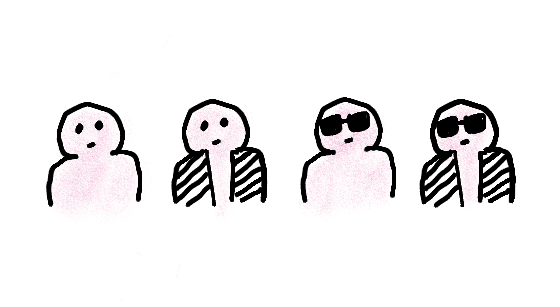
\includegraphics[keepaspectratio]{https://raw.githubusercontent.com/HowDoIGitHelp/CMSC23MDNotes/master/Markdown\%20Lecture\%20Notes\%20and\%20Lab\%20Exercises/copyright\%20free\%20drawings/Decorator.png}}
\caption{decorator}
\end{figure}

\subsection{Solution}\label{structural-patterns.md__solution}

To solve this issue, all you have to do is to apply the open/closed
principle. For every feature that can be arbitrarily added to some
simple class, you need to create a \texttt{Decorator} that extends the
features of classes using inheritance and composition at the same time.
The neat thing about this pattern is that the \texttt{Decorator}s will
have polymorphically the same type as the simple class due to
inheritance. \texttt{Decorator}s will also be able to control instances
of the simple class because of composition.

\begin{figure}
\centering
\pandocbounded{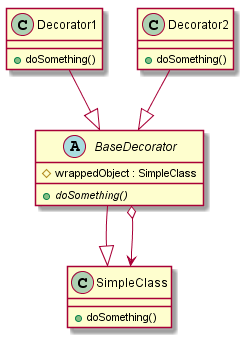
\includegraphics[keepaspectratio]{https://raw.githubusercontent.com/HowDoIGitHelp/CMSC23MDNotes/master/Markdown\%20Lecture\%20Notes\%20and\%20Lab\%20Exercises/uml/decorator.png}}
\caption{decorator}
\end{figure}

To create an instance of a \texttt{SimpleClass} decorated by
\texttt{Decorator1}, all you need to do is to wrap the
\texttt{SimpleClass} instance with an instance of \texttt{Decorator1}.
When this \texttt{Decorator1} instance, calls \texttt{doSomething()} it
calls the wrapped \texttt{SimpleClass} instance's \texttt{doSomething()}
and do some extra behavior.

\begin{Shaded}
\begin{Highlighting}[]
\CommentTok{\#Decorator1\textquotesingle{}s implementation of doSomething():}

\KeywordTok{def}\NormalTok{ doSomething(}\VariableTok{self}\NormalTok{):}
    \VariableTok{self}\NormalTok{.\_wrappedObject.doSomething()}
\NormalTok{    doSomthingExtra()}
\end{Highlighting}
\end{Shaded}

It would be handy to create a \texttt{BaseDecorator} abstract class that
is inherited by all decorators. It's not required but this class will
form a class hierarchy for all decorators. Plus, you can write all of
the common behavior and data into this class. It would be better for
this class's \texttt{doSomething()} to be abstract, since it doesn't
make sense for you to create instances of \texttt{BaseDecorator}.

\subsection{Example}\label{structural-patterns.md__example}

\subsubsection{Decorating
Sentences}\label{structural-patterns.md__decorating-sentences}

A sentence can be defined as a list of words (words are strings). The
string representation of a sentence is the concatenation of all of the
words in the list, separated by a space.

Instances of sentences can be printed with formatting:

\begin{itemize}
\item
  \textbf{bordered} - Given the sentence, \texttt{{[}"hey","there"{]}}
  it prints:

\begin{verbatim}
-----------
|hey there|
-----------
\end{verbatim}
\item
  \textbf{fancy} - Given the sentence, \texttt{{[}"hey","there"{]}} it
  prints:

\begin{verbatim}
-+hey there+-
\end{verbatim}
\item
  \textbf{uppercase} - Given the sentence, \texttt{{[}"hey","there"{]}}
  it prints:

\begin{verbatim}
HEY THERE
\end{verbatim}
\end{itemize}

The formatting of a sentence is decided during runtime. These formats
should also allow for combinations with other formats:

\begin{itemize}
\item
  \textbf{bordered fancy} - Given the sentence,
  \texttt{{[}"hey","there"{]}} it prints:

\begin{verbatim}
---------------
|-+hey there+-|
---------------
\end{verbatim}
\item
  \textbf{fancy uppercase} - Given the sentence,
  \texttt{{[}"hey","there"{]}} it prints:

\begin{verbatim}
-+HEY THERE+-
\end{verbatim}
\end{itemize}

To accomplish these features, you need to implement the decorator
pattern. Each formatting will be a decorator for \texttt{Sentence}
objects. These formats need to inherit from some abstract
\texttt{FormattedSentence} class. This abstract class is specified to
compose and inherit from sentence. The behavior that needs to be
decorated is the \texttt{\_\_str\_\_()} function since you need to
change how sentence is printed for every format.

\begin{figure}
\centering
\pandocbounded{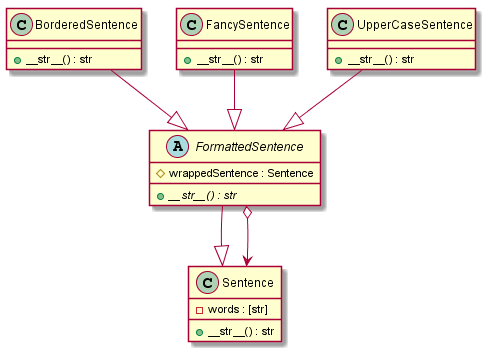
\includegraphics[keepaspectratio]{https://raw.githubusercontent.com/HowDoIGitHelp/CMSC23MDNotes/master/Markdown\%20Lecture\%20Notes\%20and\%20Lab\%20Exercises/uml/decoratorexample.png}}
\caption{decorator example}
\end{figure}

\subsection{Why this is
elegant}\label{structural-patterns.md__why-this-is-elegant}

\begin{itemize}
\tightlist
\item
  \textbf{Open/Closed Principle} - Decorators extend classes via
  inheritance. It is easier to add new decorators without touching any
  exiting code.
\item
  A class can have many variants because of diverse combinations of
  behaviors can be cleanly implemented using this pattern.
\item
  You can arbitrarily mix and match decorators without the worry of
  polymorphic incompatibility during runtime
\end{itemize}

\subsection{How to implement
it}\label{structural-patterns.md__how-to-implement-it}

\begin{enumerate}
\def\labelenumi{\arabic{enumi}.}
\tightlist
\item
  Create an abstract class \texttt{BaseDecorator} that specializes some
  \texttt{SimpleClass}. This \texttt{BaseDecorator} will also have the
  attribute \texttt{wrappedObject} which is a reference to an instance
  of the decorated \texttt{SimpleClass}. This attribute is set as
  protected so that it may be inherited by \texttt{BaseDecorator}s
  specializations. \texttt{BaseDecorator} also contains the abstract
  method \texttt{doSomething()}. This method's behavior, when invoked by
  \texttt{BaseDecorator}s specializations, changes depending on the
  decorations attached to \texttt{SimpleClass}
\item
  For every decoration, that can decorate \texttt{SimpleClass}, a
  specialization for \texttt{BaseClass} is created. These
  specializations implement \texttt{doSomething()} in a manner that
  augments/modifies \texttt{SimpleClass}'s own \texttt{doSomething()}
\end{enumerate}

\section{Adapter Pattern}\label{structural-patterns.md__adapter-pattern}

\subsection{Problem}\label{structural-patterns.md__problem-1}

As the system evolves, you'll likely encounter interfaces of instances
that are incompatible with their intended clients. These interfaces do
perform the necessary behavior, but maybe the method names are just
different. This happens quite a lot since the interface of the
dependency may be originally built for different reason. The interface
may be an external module imported on existing client code. You can just
change the incompatible interface to support the functionality you need
but this is not always possible and may introduce code duplication.

\begin{figure}
\centering
\pandocbounded{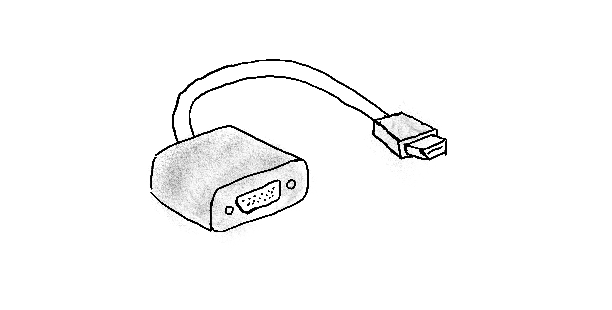
\includegraphics[keepaspectratio]{https://raw.githubusercontent.com/HowDoIGitHelp/CMSC23MDNotes/master/Markdown\%20Lecture\%20Notes\%20and\%20Lab\%20Exercises/copyright\%20free\%20drawings/Adapter.png}}
\caption{adapter}
\end{figure}

\subsection{Solution}\label{structural-patterns.md__solution-1}

In the same way a usb-c interface is usable on a usb 2.0 using an
adapter, you can use an incompatible service on a client as a compatible
instance using the adapter pattern.

Say you have an instance of \texttt{AbstractService} (it could be any
realization of \texttt{AbstractService}), that needs to be used like an
instance of \texttt{RequiredInterface} by some client. What you need to
do is to create an adapter to \texttt{AbstractService} called
\texttt{ServiceAdapter} which realizes \texttt{RequiredInterface}. To
adapt the instance of \texttt{AbstractService}, you have to compose it
inside the \texttt{ServiceAdapter}. So that \texttt{serviceMethod1()} is
adapted to \texttt{method1()}.

\begin{figure}
\centering
\pandocbounded{\includesvg[keepaspectratio]{https://raw.githubusercontent.com/HowDoIGitHelp/CMSC23MDNotes/master/Markdown\%20Lecture\%20Notes\%20and\%20Lab\%20Exercises/uml/adapter.svg}}
\caption{adapter}
\end{figure}

Whenever, a \texttt{ServiceAdapter} calls \texttt{method1()} it instead
delegates the behavior to the embedded service, which instead calls
\texttt{serviceMethod1()}

\subsection{Example}\label{structural-patterns.md__example-1}

\subsubsection{Printable
Shipments}\label{structural-patterns.md__printable-shipments}

Looking back at our previous lab exercises, some of the example classes
contain string representation but do not implement the
\texttt{\_\_str\_\_()} function. An example of this is \texttt{Shipment}
back from the factory method example. It does contain a string
representation builder called \texttt{shipmentDetails()}, but printing a
shipment is quite tedious since you have to print,
\texttt{s.shipmentDetails()}. You can replace the name of
\texttt{shipmentDetails()} to \texttt{\_\_str\_\_()} but this will
potentially affect other clients of shipment. You can add the
\texttt{\_\_str\_\_()} function which does exactly the same but this may
introduce unwanted code duplication.

The best solution for this problem is to create an adapter for shipment
called \texttt{PrintableShipment}. This adapter will realize some
\texttt{Printable} abstraction, which only contains the abstract method
\texttt{\_\_str\_\_()}.

\begin{figure}
\centering
\pandocbounded{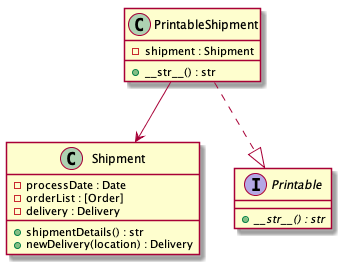
\includegraphics[keepaspectratio]{https://raw.githubusercontent.com/HowDoIGitHelp/CMSC23MDNotes/master/Markdown\%20Lecture\%20Notes\%20and\%20Lab\%20Exercises/uml/adapterexample.png}}
\caption{adapter example}
\end{figure}

\subsection{Why this is
elegant}\label{structural-patterns.md__why-this-is-elegant-1}

\begin{itemize}
\tightlist
\item
  \textbf{Open/Closed Principle} - Instead of changing existing
  incompatible interfaces, you can extend them by creating adapters.
\item
  \textbf{Interface Segregation Principle} - Instead of cluttering up
  your code with duplicate functions and unused interface methods, you
  instead create adapters only when it is needed.
\end{itemize}

\subsection{How to implement
it}\label{structural-patterns.md__how-to-implement-it-1}

\begin{enumerate}
\def\labelenumi{\arabic{enumi}.}
\tightlist
\item
  If you want an \texttt{AbstractService} to be used like a
  \texttt{RequiredInterface}, Create a \texttt{ServiceAdapter} that
  realizes \texttt{RequiredInterface} and contains an attribute
  \texttt{service} that is a reference to an instance of
  \texttt{AbstractService}.
\item
  Inside \texttt{ServiceAdapter}, the implementations of
  \texttt{RequiredInterface}'s abstract methods are merely calls to the
  methods of the reference \texttt{service}.
\end{enumerate}

\section{Composite (Optional
Read)}\label{structural-patterns.md__composite-optional-read}

\subsection{Problem}\label{structural-patterns.md__problem-2}

When entities in your system needs to be represented like trees, then
you represent them like trees.

\subsection{Solution}\label{structural-patterns.md__solution-2}

The composite pattern describes a tree structure described
polymorphically. A tree node can either be a general tree or a leaf. in
the composite pattern, a \texttt{Component} (tree node) can either be
\texttt{Composites} (general tree), or a \texttt{Leaf}. Leaves and
Composites are realizations of \texttt{Component}.

\begin{figure}
\centering
\pandocbounded{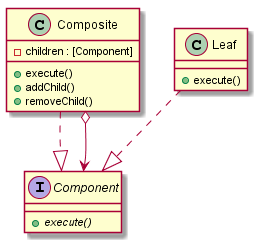
\includegraphics[keepaspectratio]{https://raw.githubusercontent.com/HowDoIGitHelp/CMSC23MDNotes/master/Markdown\%20Lecture\%20Notes\%20and\%20Lab\%20Exercises/uml/composite.png}}
\caption{composite}
\end{figure}

\subsection{Example}\label{structural-patterns.md__example-2}

\subsubsection{File System}\label{structural-patterns.md__file-system}

The file system in your computers are described using a tree structure.
The entities in your file system are either directories or files.

\begin{figure}
\centering
\pandocbounded{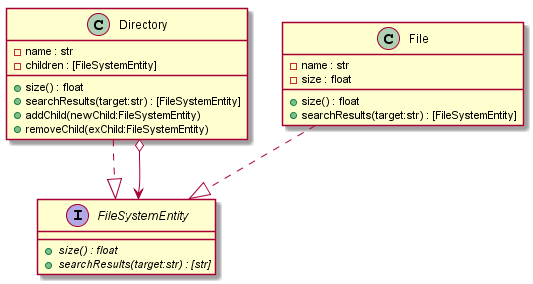
\includegraphics[keepaspectratio]{https://raw.githubusercontent.com/HowDoIGitHelp/CMSC23MDNotes/master/Markdown\%20Lecture\%20Notes\%20and\%20Lab\%20Exercises/uml/compositeexample.png}}
\caption{composite pattern}
\end{figure}

What you need to do is to implement a simulation of a file system. Each
node of the file system should be able to call the following methods:

\begin{itemize}
\tightlist
\item
  \textbf{\texttt{size()}} - the size of a \texttt{File} is based on the
  attribute size which is set during the initialization of the
  \texttt{File} instance. The size of a \texttt{Directory} is the size
  of all the \texttt{FileSystemEntities} inside it.
\item
  \textbf{\texttt{searchResults(target)}} - if used by a \texttt{File},
  if the name of the file matches the \texttt{target} it returns a list
  containing the \texttt{File}, if not it returns an empty list. If used
  by a \texttt{Directory} returns a list containing all the of the
  instances of \texttt{FileSystemEntity} (including itself) that matches
  the target inside the \texttt{Directory}.
\end{itemize}

\subsection{Why this is
elegant}\label{structural-patterns.md__why-this-is-elegant-2}

\begin{itemize}
\tightlist
\item
  \textbf{Open/Closed Principle} - You can introduce new component
  realizations in the system without touching any existing code.
\item
  Working with composite trees are easier because of the polymorphism in
  the pattern
\end{itemize}

\subsection{How to implement
it}\label{structural-patterns.md__how-to-implement-it-2}

\begin{enumerate}
\def\labelenumi{\arabic{enumi}.}
\tightlist
\item
  Create an abstraction called \texttt{Component} that contains the
  abstract methods that are supposed to be executed across all
  components.
\item
  The \texttt{Component} has two realizations, \texttt{Composite}s and
  \texttt{Leaf}s.
\item
  \texttt{Component} contains an attribute \texttt{children} which is a
  list of \texttt{Composite} instance references and the methods
  \texttt{addChild()} and \texttt{removeChild()} to attach/detach
  \texttt{Composite}s. It also has \texttt{execute()} which an
  implemented method from \texttt{Component}.
\item
  \texttt{Leaf} contains the method \texttt{execute()} as well.
\item
  When a \texttt{Composite}'s execute is invoked, it calls invokes all
  of its children's\texttt{execute()}. When \texttt{Leaf}'s execute is
  invoked it performs, leaf related behavior.
\end{enumerate}

\section{Facade (Optional
Read)}\label{structural-patterns.md__facade-optional-read}

\subsection{Problem}\label{structural-patterns.md__problem-3}

When your system becomes large enough, parts of the system which is
responsible for a single operation may involve interactions between
multiple classes. Creating flexible and maintainable systems tend to
look like this.

Looking from the outside, simple functionality (like borrowing a book or
depositing money to an account) will appear complex since it involves
multiple lines of object interaction.

\subsection{Solution}\label{structural-patterns.md__solution-3}

To solve this issue, you create a straightforward interface, that
contains methods to encapsulate complicated functionality in your
subsystem. Instead of using the internal classes to perform some
functionality, you call the facade interface's method instead.

\begin{figure}
\centering
\pandocbounded{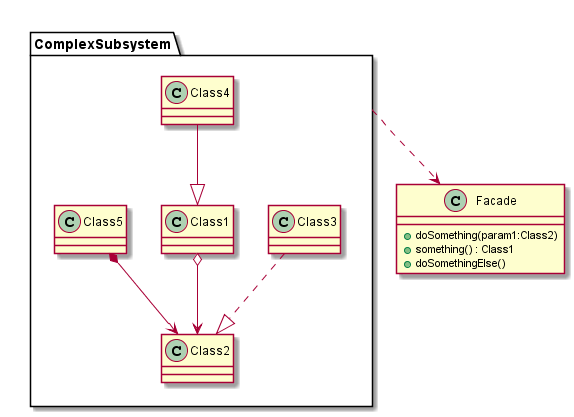
\includegraphics[keepaspectratio]{https://raw.githubusercontent.com/HowDoIGitHelp/CMSC23MDNotes/master/Markdown\%20Lecture\%20Notes\%20and\%20Lab\%20Exercises/uml/facade.png}}
\caption{facade}
\end{figure}

\subsection{Why this is
elegant}\label{structural-patterns.md__why-this-is-elegant-3}

\begin{itemize}
\tightlist
\item
  Implementing this pattern encapsulates complicated subsystem behavior
  into simple straightforward functions.
\end{itemize}

\section{Optional
Readings}\label{structural-patterns.md__optional-readings}

Shvets A. (2018)
\href{https://sourcemaking.com/design_patterns/structural_patterns}{Structural
Patterns} Accessed August 31, 2020

\chapter{Lab Exercise 1 (Structuring the Document)
(Optional)}\label{lab-exercise-1-structuring-the-document.md__lab-exercise-1-structuring-the-document-optional}

\begin{quote}
This is meant as review of imperative programming languages like C. This
Lab Exercise is optional.
\end{quote}

\section{Task}\label{lab-exercise-1-structuring-the-document.md__task}

A document is represented as a collection paragraphs, a paragraph is
represented as a collection of sentences, a sentence is represented as a
collection of words and a word is represented as a collection of
lower-case ({[}a-z{]}) and upper-case ({[}A-Z{]}) English characters.
\textbf{Create a C program that will convert a raw text document into
its component paragraphs, sentences and words}. To test your results,
queries will ask you to return a specific paragraph, sentence or word as
described below.

Words, sentences and paragraphs are represented using C structures

\subsubsection{words}\label{lab-exercise-1-structuring-the-document.md__words}

\begin{Shaded}
\begin{Highlighting}[]
\KeywordTok{struct}\NormalTok{ word }\OperatorTok{\{}
    \DataTypeTok{char}\OperatorTok{*}\NormalTok{ data}\OperatorTok{;}
\OperatorTok{\};}
\end{Highlighting}
\end{Shaded}

\subsubsection{sentences}\label{lab-exercise-1-structuring-the-document.md__sentences}

\begin{Shaded}
\begin{Highlighting}[]
\KeywordTok{struct}\NormalTok{ sentence }\OperatorTok{\{}
    \KeywordTok{struct}\NormalTok{ word}\OperatorTok{*}\NormalTok{ data}\OperatorTok{;}
    \DataTypeTok{int}\NormalTok{ word\_count}\OperatorTok{;}\CommentTok{//the number of words in a sentence}
\OperatorTok{\};}
\end{Highlighting}
\end{Shaded}

The words in a sentence are separated by one space. The last word does
not end in space ('' ``).

\subsubsection{paragraphs}\label{lab-exercise-1-structuring-the-document.md__paragraphs}

\begin{Shaded}
\begin{Highlighting}[]
\KeywordTok{struct}\NormalTok{ paragraph }\OperatorTok{\{}
    \KeywordTok{struct}\NormalTok{ sentence}\OperatorTok{*}\NormalTok{ data  }\OperatorTok{;}
    \DataTypeTok{int}\NormalTok{ sentence\_count}\OperatorTok{;}\CommentTok{//the number of sentences in a paragraph}
\OperatorTok{\};}
\end{Highlighting}
\end{Shaded}

The sentences in the paragraph are separated by one period (``.'').
There are no spaces after the period.

\subsubsection{document}\label{lab-exercise-1-structuring-the-document.md__document}

\begin{Shaded}
\begin{Highlighting}[]
\KeywordTok{struct}\NormalTok{ document }\OperatorTok{\{}
    \KeywordTok{struct}\NormalTok{ paragraph}\OperatorTok{*}\NormalTok{ data}\OperatorTok{;}
    \DataTypeTok{int}\NormalTok{ paragraph\_count}\OperatorTok{;}\CommentTok{//the number of paragraphs in document}
\OperatorTok{\};}
\end{Highlighting}
\end{Shaded}

The paragraphs in the document are separated by one newline
(\texttt{\textbackslash{}n}). The last paragraph does not end with a
newline.

The paragraphs in the document are separated by one
newline(\texttt{\textbackslash{}n}). The last paragraph does not end
with a newline.

For example:

\begin{verbatim}
Learning C is fun. 
Learning pointers is more fun.It is good to have pointers.
\end{verbatim}

The only sentence in the first paragraph could be represented as:

\begin{Shaded}
\begin{Highlighting}[]
\KeywordTok{struct}\NormalTok{ sentence first\_sentence\_in\_first\_paragraph}\OperatorTok{;}

\NormalTok{first\_sentence\_in\_first\_paragraph}\OperatorTok{.}\NormalTok{data }\OperatorTok{=} \OperatorTok{\{}\StringTok{"Learning"}\OperatorTok{,} \StringTok{"C"}\OperatorTok{,} \StringTok{"is"}\OperatorTok{,} \StringTok{"fun"}\OperatorTok{\};}
\end{Highlighting}
\end{Shaded}

The first paragraph itself could be represented as:

\begin{Shaded}
\begin{Highlighting}[]
\KeywordTok{struct}\NormalTok{ paragraph first\_paragraph}\OperatorTok{;}

\NormalTok{first\_paragraph}\OperatorTok{.}\NormalTok{data }\OperatorTok{=} \OperatorTok{\{\{}\StringTok{"Learning"}\OperatorTok{,} \StringTok{"C"}\OperatorTok{,} \StringTok{"is"}\OperatorTok{,} \StringTok{"fun"}\OperatorTok{\}\};}
\end{Highlighting}
\end{Shaded}

The first sentence in the second paragraph could be represented as:

\begin{Shaded}
\begin{Highlighting}[]
\KeywordTok{struct}\NormalTok{ sentence first\_sentence\_in\_second\_paragraph}\OperatorTok{;}

\NormalTok{first\_sentence\_in\_second\_paragraph}\OperatorTok{.}\NormalTok{data }\OperatorTok{=} \OperatorTok{\{}\StringTok{"Learning"}\OperatorTok{,} \StringTok{"pointers"}\OperatorTok{,} \StringTok{"is"}\OperatorTok{,} \StringTok{"more"}\OperatorTok{,} \StringTok{"fun"}\OperatorTok{\};}
\end{Highlighting}
\end{Shaded}

The second sentence in the second paragraph could be represented as:

\begin{Shaded}
\begin{Highlighting}[]
\KeywordTok{struct}\NormalTok{ sentence second\_sentence\_in\_second\_paragraph}\OperatorTok{;}

\NormalTok{second\_sentence\_in\_second\_paragraph}\OperatorTok{.}\NormalTok{data }\OperatorTok{=} \OperatorTok{\{}\StringTok{"It"}\OperatorTok{,} \StringTok{"is"}\OperatorTok{,} \StringTok{"good"}\OperatorTok{,} \StringTok{"to"}\OperatorTok{,} \StringTok{"have"}\OperatorTok{,} \StringTok{"pointers"}\OperatorTok{\};}
\end{Highlighting}
\end{Shaded}

The second paragraph could be represented as:

\begin{Shaded}
\begin{Highlighting}[]
\KeywordTok{struct}\NormalTok{ paragraph second\_paragraph}\OperatorTok{;}

\NormalTok{second\_paragraph}\OperatorTok{.}\NormalTok{data }\OperatorTok{=} \OperatorTok{\{\{}\StringTok{"Learning"}\OperatorTok{,} \StringTok{"pointers"}\OperatorTok{,} \StringTok{"is"}\OperatorTok{,} \StringTok{"more"}\OperatorTok{,} \StringTok{"fun"}\OperatorTok{\},} \OperatorTok{\{}\StringTok{"It"}\OperatorTok{,} \StringTok{"is"}\OperatorTok{,} \StringTok{"good"}\OperatorTok{,} \StringTok{"to"}\OperatorTok{,} \StringTok{"have"}\OperatorTok{,} \StringTok{"pointers"}\OperatorTok{\}\};}
\end{Highlighting}
\end{Shaded}

Finally, the document could be represented as:

\begin{Shaded}
\begin{Highlighting}[]
\KeywordTok{struct}\NormalTok{ document Doc}\OperatorTok{;}

\NormalTok{Doc}\OperatorTok{.}\NormalTok{data }\OperatorTok{=} \OperatorTok{\{\{\{}\StringTok{"Learning"}\OperatorTok{,} \StringTok{"C"}\OperatorTok{,} \StringTok{"is"}\OperatorTok{,} \StringTok{"fun"}\OperatorTok{\}\},} \OperatorTok{\{\{}\StringTok{"Learning"}\OperatorTok{,} \StringTok{"pointers"}\OperatorTok{,} \StringTok{"is"}\OperatorTok{,} \StringTok{"more"}\OperatorTok{,} \StringTok{"fun"}\OperatorTok{\},} \OperatorTok{\{}\StringTok{"It"}\OperatorTok{,} \StringTok{"is"}\OperatorTok{,} \StringTok{"good"}\OperatorTok{,} \StringTok{"to"}\OperatorTok{,} \StringTok{"have"}\OperatorTok{,} \StringTok{"pointers"}\OperatorTok{\}\}\};}
\end{Highlighting}
\end{Shaded}

Alicia has sent a document to her friend Teodora as a string of
characters, i.e.~represented by char* not a struct document. Help her
convert the document to struct document form by completing the following
functions:

\begin{itemize}
\tightlist
\item
  \texttt{void\ initialize\_document(char\ *text)} - to intialise the
  document. to return the paragraph in the document.
\item
  \texttt{struct\ paragraph\ kth\_paragraph(int\ k)} - return the kth
  paragraph in the document
\item
  \texttt{struct\ sentence\ kth\_sentence\_in\_mth\_paragraph(int\ k,\ int\ m)}
  - to return the kth sentence in the mth paragraph.
\item
  \texttt{struct\ word\ kth\_word\_in\_mth\_sentence\_in\_nth\_paragraph(int\ k,\ int\ m,\ int\ n)}
  - to return the kth word in the mth sentence of the nth paragraph.
\end{itemize}

\textbf{Input Format:}

The first line contains the integer \texttt{paragraph\_count}. Each of
the next \texttt{paragraph\_count} lines contains a paragraph as a
single string. The next line contains the integer \texttt{q}, the number
of queries. Each of the next \texttt{q} lines contains a query in one of
the following formats:

\begin{itemize}
\tightlist
\item
  \texttt{1\ k}: This corresponds to calling the
  function\texttt{kth\_paragraph}.
\item
  \texttt{2\ k\ m}: This corresponds to calling the function
  \texttt{kth\_sentence\_in\_mth\_paragraph}.
\item
  \texttt{3\ k\ m\ n}: This corresponds to calling the function
  \texttt{kth\_word\_in\_mth\_sentence\_in\_nth\_paragraph}.
\end{itemize}

\textbf{Constraints}

\begin{itemize}
\tightlist
\item
  The text which is passed to get\_document has words separated by a
  space, sentences separated by a period and paragraphs separated by a
  newline.
\item
  The last word in a sentence does not end with a space.
\item
  The last paragraph does not end with a newline.
\item
  The words contain only upper-case and lower-case English letters.
\item
  1 \textless= number of characters in the entire document \textless=
  1000 .
\item
  1 \textless= number of paragraphs in the entire document \textless= 5.
\end{itemize}

\textbf{Output Format}

Print the paragraph, sentence or the word corresponding to the query to
check the logic of your code.

\textbf{Sample Input 0}

\begin{Shaded}
\begin{Highlighting}[]
\DecValTok{2}
\NormalTok{Learning C is fun}\OperatorTok{.}
\NormalTok{Learning pointers is more fun}\OperatorTok{.}\NormalTok{It is good to have pointers}\OperatorTok{.}
\DecValTok{3}
\DecValTok{1} \DecValTok{2}
\DecValTok{2} \DecValTok{1} \DecValTok{1}
\DecValTok{3} \DecValTok{1} \DecValTok{1} \DecValTok{1}
\end{Highlighting}
\end{Shaded}

\textbf{Sample Output 0}

\begin{Shaded}
\begin{Highlighting}[]
\NormalTok{Learning pointers is more fun}\OperatorTok{.}\NormalTok{It is good to have pointers}\OperatorTok{.}
\NormalTok{Learning C is fun}
\NormalTok{Learning}
\end{Highlighting}
\end{Shaded}

\textbf{Explanation 0}

\begin{itemize}
\tightlist
\item
  The first query returns the second paragraph.\\
\item
  The second query returns the first sentence of the first paragraph.
\item
  The third query returns the first word of the first sentence of the
  first paragraph
\end{itemize}

\section{Assessment
Criteria}\label{lab-exercise-1-structuring-the-document.md__assessment-criteria}

\emph{This exercise is optional}

\chapter{Lab Exercise
2}\label{lab-exercise-2-exploring-haskell.md__lab-exercise-2}

\section{Task}\label{lab-exercise-2-exploring-haskell.md__task}

We've discussed functional programming paradigms using the language
haskell as a representative. For this exercise, you'll familiarize
yourselves on how to write pure functions in haskell. \textbf{Create a
haskell file (``.hs'') containing the following functions below.}

For those of you using REPL's haskell compiler add the following snippet
of code the the bottom of your function definitions. For those of you
using ghc in your computers ignore this.

\begin{Shaded}
\begin{Highlighting}[]
\OtherTok{main ::} \DataTypeTok{IO}\NormalTok{ ()}
\NormalTok{main }\OtherTok{=} \FunctionTok{return}\NormalTok{ ()}
\end{Highlighting}
\end{Shaded}

\subsubsection{Easy
functions}\label{lab-exercise-2-exploring-haskell.md__easy-functions}

\begin{itemize}
\tightlist
\item
  \texttt{cube\ ::\ Int\ -\textgreater{}\ Int} - Consumes an integer and
  produces the cube of that integer
\item
  \texttt{double\ ::\ Int\ -\textgreater{}\ Int} - Consumes an integer
  and produces the 2 times that integer
\end{itemize}

\subsubsection{\texorpdfstring{\textbf{Recursive
Functions}}{Recursive Functions}}\label{lab-exercise-2-exploring-haskell.md__recursive-functions}

\begin{itemize}
\item
  \texttt{modulus\ ::\ Int\ -\textgreater{}\ Int\ -\textgreater{}\ Int}
  - Consumes two integers \(x\) and \(m\) and produces \(x \mod m\)
\item
  \texttt{factorial\ ::\ Int\ -\textgreater{}\ Int} - Consumes an
  integer and produces the factorial of the integer
\item
  \texttt{summation\ ::\ Int\ -\textgreater{}\ Int} - Consumes a natural
  number and produces the summation of numbers from 1 to
  n.~\(\sum_{i=1}^{n}{i}\).

\begin{Shaded}
\begin{Highlighting}[]
\OtherTok{summation ::} \DataTypeTok{Int} \OtherTok{{-}\textgreater{}} \DataTypeTok{Int}
\NormalTok{summation n }\OtherTok{=} \KeywordTok{if}\NormalTok{ (n }\OperatorTok{\textless{}=} \DecValTok{1}\NormalTok{) }\KeywordTok{then}\NormalTok{ n }\KeywordTok{else}\NormalTok{ (n }\OperatorTok{+}\NormalTok{ (summation (n}\OperatorTok{{-}}\DecValTok{1}\NormalTok{)))}
\end{Highlighting}
\end{Shaded}
\end{itemize}

\subsubsection{Higher order
function}\label{lab-exercise-2-exploring-haskell.md__higher-order-function}

\begin{itemize}
\tightlist
\item
  \texttt{compose\ ::\ (Int\ -\textgreater{}\ Int)\ -\textgreater{}\ (Int\ -\textgreater{}\ Int)\ -\textgreater{}\ (Int\ -\textgreater{}\ Int)}
  - Consumes two functions \(f : \mathbb{Z} \to \mathbb{Z}\), and
  \(g:  \mathbb{Z} \to \mathbb{Z}\) and produces the function
  \(f \circ g\).
\item
  \texttt{subtractMaker\ ::\ Int\ -\textgreater{}\ (Int\ -\textgreater{}\ Int)}
  - Consumes an integer \(x\) and produces a function that consumes an
  integer \(y\) and produces \(x-y\)
\item
  \texttt{applyNTimes\ ::\ (Int\ -\textgreater{}\ Int)\ -\textgreater{}\ Int\ -\textgreater{}\ Int\ -\textgreater{}\ Int}
  - Consumes a function \(f: \mathbb{Z} \to \mathbb{Z}\) and and two
  integers \(n\) and \(x\). \texttt{applyNTimes} produces an integer
  which is the result of the function applied to \(x\), \(n\)-times. If
  \(n\) is less than or equal to 0 it must produce zero applications of
  \(f\) therefore it produces \(x\).
\end{itemize}

\section{Assessment
Criteria}\label{lab-exercise-2-exploring-haskell.md__assessment-criteria}

\begin{itemize}
\tightlist
\item
  Completeness of haskell functions - 40
\end{itemize}

\chapter{Lab Exercise 3 (Higher Order Functions for List
Comprehension)}\label{lab-exercise-3-higher-order-functions.md__lab-exercise-3-higher-order-functions-for-list-comprehension}

\section{Task}\label{lab-exercise-3-higher-order-functions.md__task}

After familiarizing yourselves with haskell functions, lets move on to
list comprehension functions. These functions are probably functional
programming's most well-known contribution to other paradigms. Although
these functions are already built in inside haskell, you are going to
make your own versions of it. \textbf{Create a haskell file (``.hs'')
containing the following functions below.} One of them
(\texttt{my\_filter}) is already written for you but please still
include this function in your haskell file.

\subsection{Lists in
Haskell}\label{lab-exercise-3-higher-order-functions.md__lists-in-haskell}

Before you start implementing the functions in this exercise, you need
to understand how lists work in Haskell. Haskell lists are written like
a list in math. The Haskell list:

\begin{Shaded}
\begin{Highlighting}[]
\NormalTok{[}\DecValTok{1}\NormalTok{,}\DecValTok{2}\NormalTok{,}\DecValTok{3}\NormalTok{,}\DecValTok{4}\NormalTok{,}\DecValTok{5}\NormalTok{]}
\end{Highlighting}
\end{Shaded}

is basically equivalent to the list: \[
[1,2,3,4,5]
\] One of the most important things about lists is that you can access
the list as a whole and you can access the elements inside the list. One
thing you can do is you can concatenate lists using the
\textbf{\texttt{++}} function:

\begin{Shaded}
\begin{Highlighting}[]
\NormalTok{ghci}\OperatorTok{\textgreater{}}\NormalTok{ [}\DecValTok{1}\NormalTok{,}\DecValTok{2}\NormalTok{,}\DecValTok{3}\NormalTok{,}\DecValTok{4}\NormalTok{,}\DecValTok{5}\NormalTok{] }\OperatorTok{++}\NormalTok{ [}\DecValTok{6}\NormalTok{,}\DecValTok{7}\NormalTok{,}\DecValTok{8}\NormalTok{]}
\NormalTok{[}\DecValTok{1}\NormalTok{,}\DecValTok{2}\NormalTok{,}\DecValTok{3}\NormalTok{,}\DecValTok{4}\NormalTok{,}\DecValTok{5}\NormalTok{,}\DecValTok{6}\NormalTok{,}\DecValTok{7}\NormalTok{,}\DecValTok{8}\NormalTok{]}
\end{Highlighting}
\end{Shaded}

You can find the length of the list using the \textbf{\texttt{length}}
function:

\begin{Shaded}
\begin{Highlighting}[]
\NormalTok{ghci}\OperatorTok{\textgreater{}} \FunctionTok{length}\NormalTok{ [}\DecValTok{1}\NormalTok{,}\DecValTok{2}\NormalTok{,}\DecValTok{3}\NormalTok{,}\DecValTok{4}\NormalTok{,}\DecValTok{5}\NormalTok{]}
\DecValTok{5}
\end{Highlighting}
\end{Shaded}

These are the different ways you can access the elements of the list and
the sublists in the list:

\textbf{\texttt{head}} takes a list and returns the first element of the
list

\begin{Shaded}
\begin{Highlighting}[]
\NormalTok{ghci}\OperatorTok{\textgreater{}} \FunctionTok{head}\NormalTok{ [}\DecValTok{1}\NormalTok{,}\DecValTok{2}\NormalTok{,}\DecValTok{3}\NormalTok{,}\DecValTok{4}\NormalTok{,}\DecValTok{5}\NormalTok{]}
\DecValTok{1}
\end{Highlighting}
\end{Shaded}

\textbf{\texttt{tail}} takes a list and returns the same list except the
first element of the list

\begin{Shaded}
\begin{Highlighting}[]
\NormalTok{ghci}\OperatorTok{\textgreater{}} \FunctionTok{tail}\NormalTok{ [}\DecValTok{1}\NormalTok{,}\DecValTok{2}\NormalTok{,}\DecValTok{3}\NormalTok{,}\DecValTok{4}\NormalTok{,}\DecValTok{5}\NormalTok{]}
\NormalTok{[}\DecValTok{2}\NormalTok{,}\DecValTok{3}\NormalTok{,}\DecValTok{4}\NormalTok{,}\DecValTok{5}\NormalTok{]}
\end{Highlighting}
\end{Shaded}

\textbf{\texttt{init}} takes a list and returns the same list except the
last element of the list

\begin{Shaded}
\begin{Highlighting}[]
\NormalTok{ghci}\OperatorTok{\textgreater{}} \FunctionTok{init}\NormalTok{ [}\DecValTok{1}\NormalTok{,}\DecValTok{2}\NormalTok{,}\DecValTok{3}\NormalTok{,}\DecValTok{4}\NormalTok{,}\DecValTok{5}\NormalTok{]}
\NormalTok{[}\DecValTok{1}\NormalTok{,}\DecValTok{2}\NormalTok{,}\DecValTok{3}\NormalTok{,}\DecValTok{4}\NormalTok{]}
\end{Highlighting}
\end{Shaded}

\textbf{\texttt{last}} takes a list and returns the last element in the
list

\begin{Shaded}
\begin{Highlighting}[]
\NormalTok{ghci}\OperatorTok{\textgreater{}} \FunctionTok{last}\NormalTok{ [}\DecValTok{1}\NormalTok{,}\DecValTok{2}\NormalTok{,}\DecValTok{3}\NormalTok{,}\DecValTok{4}\NormalTok{,}\DecValTok{5}\NormalTok{]}
\DecValTok{5}
\end{Highlighting}
\end{Shaded}

Using these functions you can traverse a list using the head-tail
recipe. For example, if you want to add 1 to each of the elements of the
array:

\begin{Shaded}
\begin{Highlighting}[]
\OtherTok{addone ::}\NormalTok{ [}\DataTypeTok{Int}\NormalTok{] }\OtherTok{{-}\textgreater{}}\NormalTok{ [}\DataTypeTok{Int}\NormalTok{]}
\NormalTok{addone l }\OtherTok{=} 
  \KeywordTok{if} \FunctionTok{length}\NormalTok{ l }\OperatorTok{==} \DecValTok{0} \KeywordTok{then}\NormalTok{ []}
  \KeywordTok{else}\NormalTok{ [(}\FunctionTok{head}\NormalTok{ l) }\OperatorTok{+} \DecValTok{1}\NormalTok{] }\OperatorTok{++}\NormalTok{ addone (}\FunctionTok{tail}\NormalTok{ l)}
\end{Highlighting}
\end{Shaded}

Let's dissect this function one by one, for the first line you can see
the type signature \texttt{{[}Int{]}-\textgreater{}{[}Int{]}} meaning
\texttt{addone} accepts a list of \texttt{Int}s and returns a list of
\texttt{Int}s. Any type \texttt{a} surrounded by brackets is a list of
\texttt{a}s (\texttt{{[}a{]}} is a list of \texttt{a}'s,
\texttt{{[}Char{]}} is a list of \texttt{Chars},
\texttt{{[}{[}Int{]}{]}} is a list of \texttt{{[}Int{]}}s or a list of
list of \texttt{Int}s).

In the second line were binding the list we are passing to \texttt{l}.

The third line refers to the base case, this happens when the list is
empty. When writing the base case, think about the most simple possible
list the function may be applied to. The simplest case would be an empty
list. When the list is empty we return \texttt{{[}{]}} which refers to
an empty list.

And finally the last line refers to the general case. Here we are see
the subexpression \texttt{{[}(head\ l)\ +\ 1{]}} which is a list
containing one element namely, the first element of the list plus 1. And
then we are concatenating this one element list to the result of the
call \texttt{addone\ (tail\ l)} which is a recursive call to the rest of
add one to the \texttt{tail} of l (or the rest of \texttt{l}). Assuming
\texttt{addone} works perfectly, the recursive call
\texttt{addone\ (tail\ l)} will return the tail of the \texttt{l} but
the elements are added with one. By concatenating
\texttt{{[}(head\ l)\ +\ 1{]}} with the result of this recursive call,
we complete the desired result.

\begin{itemize}
\item
  Implement the higher order functions,
  \texttt{my\_map},\texttt{my\_filter}, and \texttt{my\_foldl} and
  \texttt{my\_foldr}, \texttt{my\_zip}

  \begin{itemize}
  \item
    \textbf{\texttt{my\_map\ ::\ (a\ -\textgreater{}\ b)\ -\textgreater{}\ {[}a{]}\ -\textgreater{}\ {[}b{]}}}
    - The \texttt{my\_map} function accepts a function \[f\] and a list
    (with elements of type \texttt{A}) \[l=[l_1,l_2,l_3,...,l_n]\]. It
    returns the list (with elements of type \texttt{B}):
    \[l'=[f(l_1),f(l_2),f(l_3),...,f(l_4)]\]. The new list
    \texttt{my\_map} produces is a list which is the image of \texttt{l}
    from the function \texttt{f}.
  \item
    \textbf{\texttt{my\_filter\ ::\ (a\ -\textgreater{}\ Bool)\ -\textgreater{}\ {[}a{]}\ -\textgreater{}\ {[}a{]}}}
    - The \texttt{my\_filter} function accepts a predicate \[f\] and a
    list \[l=[l_1,l_2,l_3,\cdots,l_n]\]. \texttt{my\_filter} returns a
    new list \[l'\] such that the contents satisfy \[f(l_i)\] is true,
    retaining the order it appears in \[l\].

    BONUS (here's \texttt{my\_filter} solved for you, use this as a
    guide):

\begin{Shaded}
\begin{Highlighting}[]
\OtherTok{my\_filter ::}\NormalTok{ (a }\OtherTok{{-}\textgreater{}} \DataTypeTok{Bool}\NormalTok{) }\OtherTok{{-}\textgreater{}}\NormalTok{ [a] }\OtherTok{{-}\textgreater{}}\NormalTok{ [a]}
\NormalTok{my\_filter p l }\OtherTok{=} 
    \KeywordTok{if} \FunctionTok{length}\NormalTok{ l }\OperatorTok{==} \DecValTok{0} \KeywordTok{then}\NormalTok{ []}
    \KeywordTok{else}\NormalTok{ (}\KeywordTok{if}\NormalTok{ p (}\FunctionTok{head}\NormalTok{ l) }\KeywordTok{then}\NormalTok{ [}\FunctionTok{head}\NormalTok{ l] }\KeywordTok{else}\NormalTok{ []) }\OperatorTok{++}\NormalTok{ my\_filter p (}\FunctionTok{tail}\NormalTok{ l)}
\end{Highlighting}
\end{Shaded}

    The notable part of this \texttt{my\_filter}'s body is the last. The
    non-base case clause evaluates the following line

\begin{Shaded}
\begin{Highlighting}[]
\NormalTok{(}\KeywordTok{if}\NormalTok{ p (}\FunctionTok{head}\NormalTok{ l) }\KeywordTok{then}\NormalTok{ [}\FunctionTok{head}\NormalTok{ l] }\KeywordTok{else}\NormalTok{ []) }\OperatorTok{++}\NormalTok{ my\_filter p (}\FunctionTok{tail}\NormalTok{ l)}
\end{Highlighting}
\end{Shaded}

    The first part is the if-then-else clause
    \texttt{(if\ p\ (head\ l)\ then\ {[}head\ l{]}\ else\ {[}{]})} which
    evaluates to either the list containing the first element of
    \texttt{l} (\texttt{{[}head\ l{]}}) or an empty list
    (\texttt{{[}{]}}). If the first element (\texttt{head\ l}) satisfies
    the predicate \texttt{p} (therefore the if clause contains the
    expression \texttt{p\ (head\ l)} ), then the if-then-else clause
    evaluates to \texttt{{[}head\ l{]}} otherwise it evaluates to
    \texttt{{[}{]}}. Whatever, the \texttt{if-then-else} clause
    evaluates to is then concatenated to the result of the recursive
    call to the tail of \texttt{l} (\texttt{my\_filter\ p\ (tail\ l)}).
    Every time the function recurses, the first element is either
    concatenated or not concatenated to the rest of the list, this
    filtering out all elements that do not satisfy the predicate.
  \item
    \textbf{\texttt{my\_foldl\ ::\ (a\ -\textgreater{}\ a\ -\textgreater{}\ a)\ -\textgreater{}\ a\ -\textgreater{}\ {[}a{]}\ -\textgreater{}\ a}}
    - The \texttt{my\_foldl} function accepts a function \[f\], a list
    \[l=[l_1,l_2,l_3,...,l_n]\] and an initial value \[u\]. The
    \texttt{my\_foldl} function returns the value
    \[f(\cdots f(f(f(u,l_1), l_2),l_3) \cdots, l_n)\]. If \[l\] is empty
    \texttt{my\_foldl} returns \[u\].
  \item
    \textbf{\texttt{my\_foldr\ ::\ (a\ -\textgreater{}\ a\ -\textgreater{}\ a)\ -\textgreater{}\ a\ -\textgreater{}\ {[}a{]}\ -\textgreater{}\ a}}
    - The \texttt{my\_foldr} function accepts a function \[f\], a list
    \[l=[l_1,l_2,l_3,...,l_n]\] and an initial value \[u\]. The
    \texttt{my\_foldr} function returns the value
    \[f(l_1,f(l_2,f(l_3,\cdots f(l_n,u) \cdots )))\]. If \[l\] is empty
    `my\_foldlr returns \[u\].
  \item
    \textbf{\texttt{my\_zip\ ::\ (a\ -\textgreater{}\ b\ -\textgreater{}\ c)\ -\textgreater{}\ {[}a{]}\ -\textgreater{}\ {[}b{]}\ -\textgreater{}\ {[}c{]}}}
    - The \texttt{my\_zip} function accepts a function \[f\] and two
    lists \[l=[l_1,l_2,l_3,...,l_n]\], \[m=[m_1,m_2,m_3,...,m_n]\] and
    returns a new list,
    \[k=[f(l_1,m_1),f(l_2,m_2),f(l_3,m_3),\cdots,f(l_n,m_n)]\]
  \end{itemize}
\item
  Without using loops (use the functions above instead), write the
  following functions.

  \begin{itemize}
  \item
    \texttt{composeAll\ ::\ {[}(a\ -\textgreater{}\ a){]}\ -\textgreater{}\ (a\ -\textgreater{}\ a)}:
    given a list of \texttt{(a\ -\textgreater{}\ a)} functions, return
    the composition of all of them. For example, given the list of
    functions \[[f_1,f_2,f_3,\cdots, f_n]\], it produces the composition
    \(f_1 \circ f_2 \circ f_3 \circ \cdots \circ f_n\).
  \item
    \texttt{isPrime\ ::\ Int\ -\textgreater{}\ Bool} - Given an integer
    return true if the number is prime, false otherwise (hint: you can
    use \texttt{isDivisible} and \texttt{candidateFactors} along with
    the higher order functions above).
  \item
    \texttt{sumOfSquares\ ::\ {[}Int{]}\ -\textgreater{}\ Int} - Given a
    list of numbers, return the sum of the squares of the numbers
  \item
    \texttt{wholeName\ ::\ {[}String{]}\ -\textgreater{}\ {[}String{]}\ -\textgreater{}\ {[}String{]}\ -\textgreater{}\ {[}String{]}}
    - Given three lists, a list of first names, A, a list of middle
    names B, and a list of surnames C. Return a list of whole name
    strings (list of chars)
    (\texttt{{[}firstname{]}\ {[}middle\ initial{]}.\ {[}lastname{]}})
    where the length of the string (including spaces and period) is an
    even number. Example

\begin{Shaded}
\begin{Highlighting}[]
\NormalTok{ghci}\OperatorTok{\textgreater{}}\NormalTok{ wholeName [}\StringTok{"Foo"}\NormalTok{, }\StringTok{"Bar"}\NormalTok{, }\StringTok{"Foo"}\NormalTok{] [}\StringTok{"Middle"}\NormalTok{, }\StringTok{"Center"}\NormalTok{, }\StringTok{"Name"}\NormalTok{] [}\StringTok{"Lastn"}\NormalTok{, }\StringTok{"Surname"}\NormalTok{, }\StringTok{"Abcd"}\NormalTok{]}
\NormalTok{[}\StringTok{"Foo M. Lastn"}\NormalTok{, }\StringTok{"Bar C. Surname"}\NormalTok{]}
\end{Highlighting}
\end{Shaded}

    (``Foo N. Abcd'' is filtered out because it has 11 characters)
  \end{itemize}
\end{itemize}

\section{Assessment
Criteria}\label{lab-exercise-3-higher-order-functions.md__assessment-criteria}

\begin{itemize}
\tightlist
\item
  Completeness of haskell functions - 35
\end{itemize}

\chapter{Lab Exercise 4 (Drama in the Clue
Mansion)}\label{lab-exercise-4-drama-in-the-clue-mansion.md__lab-exercise-4-drama-in-the-clue-mansion}

\section{Task}\label{lab-exercise-4-drama-in-the-clue-mansion.md__task}

You can use a knowledge base to represent human relationship networks.
This is what you will be doing for this exercise. I've written a few
example facts, and rules as your guide below. \textbf{Create a prolog
knowledge base (``.pl'') containing the following facts. Also, create a
text file containing the answers to to queries you can below.}

\begin{itemize}
\tightlist
\item
  Create a knowledge base and place them all inside a file with a
  ``.pl'' extension

  \begin{enumerate}
  \def\labelenumi{\arabic{enumi}.}
  \tightlist
  \item
    \emph{Miss Scarlet, Mrs.~White, Mrs.~Peacock, Dr.~Orchid are female}
  \item
    Prof.~Plum, Colonel Mustard, and Rev.~Green are all male
  \item
    \emph{Miss Scarlet hates Rev.~Green.}
  \item
    Rev.~Green hates Miss Scarlet
  \item
    Prof.~Plum and Mrs.~White hate each other.
  \item
    Col. Mustard hates all females and Prof.~Plum.
  \item
    Miss Scarlet and Mrs.~Peacock both like Dr.~Orchid.
  \item
    Dr.~Orchid likes Mrs.~Peacock
  \item
    Miss Scarlet likes Mrs.~White
  \item
    Miss Scarlet and Prof.~Plum like each other.
  \item
    Prof.~Plum likes everyone Col. Mustard hates.
  \item
    \emph{People who hate each other are enemies}
  \item
    People who like each other are friends
  \item
    The enemies of someone's enemies is his/her friend.
  \end{enumerate}
\item
  Based on the knowledge base you created, ask it the following queries
  by running \texttt{swipl\ labExer4.pl}. Write the solutions to each
  query into a text file.

  \begin{enumerate}
  \def\labelenumi{\arabic{enumi}.}
  \tightlist
  \item
    \emph{Which pairs are enemies?}
  \item
    Which pairs are friends?
  \item
    Which people are liked by Prof.~Plum.
  \item
    Which people like themselves?
  \item
    Which males are liked by females? (this query must be written as a
    conjunction)
  \item
    Which people are hated by the one they like? (this query must be
    written as a conjunction)
  \end{enumerate}
\end{itemize}

\section{Some example facts and rules as
guide}\label{lab-exercise-4-drama-in-the-clue-mansion.md__some-example-facts-and-rules-as-guide}

(don't skip writing these facts and rules in your knowledge base so that
it works)

\begin{verbatim}
%Propositions in item 1
female(scarlet).
female(peacock).
female(orchid).

%Proposition in item 2 (Miss Scarlet hates Rev. Green)
hates(scarlet, green).

%Rule in item 12 (People who hate each other are enemies)
enemies(X,Y) :- hates(X,Y), hates(Y,X).
\end{verbatim}

\section{Some example
queries}\label{lab-exercise-4-drama-in-the-clue-mansion.md__some-example-queries}

(Although the answers are already provided here, still, copy them on the
text file containing the answers from the other queries).

You should get similar answers to the following queries

Which pairs are enemies?

\begin{verbatim}
?- enemies(A,B).
\end{verbatim}

\begin{verbatim}
A = scarlet,
B = green ;
A = green,
B = scarlet ;
A = plum,
B = white ;
A = white,
B = plum ;
false.
\end{verbatim}

Which males are liked by females?

\begin{verbatim}
?- likes(A,B), female(A), male(B).
\end{verbatim}

\begin{verbatim}
A = scarlet,
B = plum ;
false.
\end{verbatim}

\section{Assessment
Criteria}\label{lab-exercise-4-drama-in-the-clue-mansion.md__assessment-criteria}

\begin{itemize}
\tightlist
\item
  Completeness of knowledge base - 20
\item
  Accuracy of query results - 20
\end{itemize}

\chapter{Lab Exercise 5
(Snakes)}\label{lab-exercise-5-snakes.md__lab-exercise-5-snakes}

Implement the following functions:

\subsubsection{doubledInt}\label{lab-exercise-5-snakes.md__doubledint}

accepts an int and return the double of that int

\begin{Shaded}
\begin{Highlighting}[]
\KeywordTok{def}\NormalTok{ doubledInt(x:}\BuiltInTok{int}\NormalTok{) }\OperatorTok{{-}\textgreater{}} \BuiltInTok{int}\NormalTok{:}
    \ControlFlowTok{pass}
\end{Highlighting}
\end{Shaded}

\subsubsection{largest}\label{lab-exercise-5-snakes.md__largest}

accepts two floats and returns the larger value

\begin{Shaded}
\begin{Highlighting}[]
\KeywordTok{def}\NormalTok{ largest(x:}\BuiltInTok{float}\NormalTok{,y:}\BuiltInTok{float}\NormalTok{) }\OperatorTok{{-}\textgreater{}} \BuiltInTok{float}\NormalTok{:}
    \ControlFlowTok{pass}
\end{Highlighting}
\end{Shaded}

\subsubsection{verticalLine}\label{lab-exercise-5-snakes.md__verticalline}

accepts two (float,float) tuples which represent two points in a
cartesian plane (x,y) and returns true if the points describe a vertical
line and false otherwise

\begin{Shaded}
\begin{Highlighting}[]
\KeywordTok{def}\NormalTok{ verticalLine(a:}\BuiltInTok{tuple}\NormalTok{[}\BuiltInTok{float}\NormalTok{,}\BuiltInTok{float}\NormalTok{],b:[}\BuiltInTok{float}\NormalTok{,}\BuiltInTok{float}\NormalTok{] }\OperatorTok{{-}\textgreater{}} \BuiltInTok{bool}\NormalTok{:}
    \ControlFlowTok{pass}
\end{Highlighting}
\end{Shaded}

\subsubsection{primes}\label{lab-exercise-5-snakes.md__primes}

accepts an integer n and returns the first n primes

\begin{Shaded}
\begin{Highlighting}[]
\KeywordTok{def}\NormalTok{ primes(n:}\BuiltInTok{int}\NormalTok{) }\OperatorTok{{-}\textgreater{}} \BuiltInTok{list}\NormalTok{[}\BuiltInTok{int}\NormalTok{]:}
    \ControlFlowTok{pass}
\end{Highlighting}
\end{Shaded}

\subsubsection{fibonacci}\label{lab-exercise-5-snakes.md__fibonacci}

accepts an integer n and returns a the list containing the first n
elements of fibonacci sequence (starting with 0 and 1)

\begin{Shaded}
\begin{Highlighting}[]
\KeywordTok{def}\NormalTok{ fibonacci(n:}\BuiltInTok{int}\NormalTok{) }\OperatorTok{{-}\textgreater{}} \BuiltInTok{list}\NormalTok{[}\BuiltInTok{int}\NormalTok{]:}
    \ControlFlowTok{pass}
\end{Highlighting}
\end{Shaded}

\subsubsection{sortedIntegers}\label{lab-exercise-5-snakes.md__sortedintegers}

accepts a list of integers and sorts it from smallest to highest, please
do not use python's builtin sort, implement your own sort function

\begin{Shaded}
\begin{Highlighting}[]
\KeywordTok{def}\NormalTok{ sortedIntegers(l:[}\BuiltInTok{int}\NormalTok{]) }\OperatorTok{{-}\textgreater{}} \BuiltInTok{list}\NormalTok{[}\BuiltInTok{int}\NormalTok{]:}
    \ControlFlowTok{pass}
\end{Highlighting}
\end{Shaded}

\subsubsection{sublists}\label{lab-exercise-5-snakes.md__sublists}

accepts a list of integers and returns all the sublists of the list.
Sublists are contigous chunks of a list (including an empty list and the
list itself). \texttt{{[}1,2{]}}, \texttt{{[}2{]}}, \texttt{{[}{]}},
\texttt{{[}2,3,4{]}}, and \texttt{{[}1,2,3,4,5{]}} are sublists of
\texttt{{[}1,2,3,4,5{]}} but \texttt{{[}3,5{]}} and
\texttt{{[}1,2,3,4,6{]}} are not.

\begin{Shaded}
\begin{Highlighting}[]
\KeywordTok{def}\NormalTok{ sublists(l:}\BuiltInTok{list}\NormalTok{[}\BuiltInTok{int}\NormalTok{]) }\OperatorTok{{-}\textgreater{}} \BuiltInTok{list}\NormalTok{[}\BuiltInTok{list}\NormalTok{[}\BuiltInTok{int}\NormalTok{]]:}
    \ControlFlowTok{pass}
\end{Highlighting}
\end{Shaded}

\chapter{Lab Exercise 6 (Borrowing from the
Library)}\label{lab-exercise-6-borrowing-from-the-library.md__lab-exercise-6-borrowing-from-the-library}

\section{Task}\label{lab-exercise-6-borrowing-from-the-library.md__task}

You are to implement the following system. This system represents the
borrowing and returning functions of a library. Here's the class
diagram. \textbf{Edit the python file that came with this document.} The
edited file is what you are going to submit.

\begin{figure}
\centering
\pandocbounded{\includegraphics[keepaspectratio]{https://i.imgur.com/9zHBavi.png}}
\caption{UML}
\end{figure}

There is some code already written for you here:

\begin{Shaded}
\begin{Highlighting}[]
\ImportTok{from}\NormalTok{ abc }\ImportTok{import}\NormalTok{ ABC, abstractmethod}
\ImportTok{from}\NormalTok{ datetime }\ImportTok{import}\NormalTok{ date,timedelta}

\KeywordTok{def}\NormalTok{ daysBetween(date1:date, date2:date) }\OperatorTok{{-}\textgreater{}} \BuiltInTok{int}\NormalTok{:}
\NormalTok{    difference:}\BuiltInTok{int} \OperatorTok{=}\NormalTok{ date1 }\OperatorTok{{-}}\NormalTok{  date2}
    \ControlFlowTok{return}\NormalTok{ difference.days}

\KeywordTok{class}\NormalTok{ Page:}
    \KeywordTok{def} \FunctionTok{\_\_init\_\_}\NormalTok{(}\VariableTok{self}\NormalTok{, sectionHeader:}\BuiltInTok{str}\NormalTok{, body: }\BuiltInTok{str}\NormalTok{):}
        \VariableTok{self}\NormalTok{.\_\_sectionHeader }\OperatorTok{=}\NormalTok{ sectionHeader}
        \VariableTok{self}\NormalTok{.\_\_body }\OperatorTok{=}\NormalTok{ body}

\KeywordTok{class}\NormalTok{ BorrowableItem(ABC):}
    \AttributeTok{@abstractmethod}
    \KeywordTok{def}\NormalTok{ uniqueItemId(}\VariableTok{self}\NormalTok{) }\OperatorTok{{-}\textgreater{}} \BuiltInTok{int}\NormalTok{:}
        \ControlFlowTok{pass}
    \AttributeTok{@abstractmethod}
    \KeywordTok{def}\NormalTok{ commonName(}\VariableTok{self}\NormalTok{) }\OperatorTok{{-}\textgreater{}} \BuiltInTok{str}\NormalTok{:}
        \ControlFlowTok{pass}



\KeywordTok{class}\NormalTok{ Book(BorrowableItem):}
    \KeywordTok{def} \FunctionTok{\_\_init\_\_}\NormalTok{(}\VariableTok{self}\NormalTok{, bookId:}\BuiltInTok{int}\NormalTok{, title:}\BuiltInTok{str}\NormalTok{, author:}\BuiltInTok{str}\NormalTok{, publishDate:date, pages: }\BuiltInTok{list}\NormalTok{[Page]):}
        \VariableTok{self}\NormalTok{.\_\_bookId }\OperatorTok{=}\NormalTok{ bookId}
        \VariableTok{self}\NormalTok{.\_\_title }\OperatorTok{=}\NormalTok{ title}
        \VariableTok{self}\NormalTok{.\_\_publishDate }\OperatorTok{=}\NormalTok{ publishDate}
        \VariableTok{self}\NormalTok{.\_\_author }\OperatorTok{=}\NormalTok{ author}
        \VariableTok{self}\NormalTok{.\_\_pages }\OperatorTok{=}\NormalTok{ pages}
    \KeywordTok{def}\NormalTok{ coverInfo(}\VariableTok{self}\NormalTok{) }\OperatorTok{{-}\textgreater{}} \BuiltInTok{str}\NormalTok{:}
        \ControlFlowTok{return} \StringTok{"Title: "} \OperatorTok{+} \VariableTok{self}\NormalTok{.\_\_title }\OperatorTok{+} \StringTok{"}\CharTok{\textbackslash{}n}\StringTok{Author: "} \OperatorTok{+} \VariableTok{self}\NormalTok{.\_\_author}
    \KeywordTok{def}\NormalTok{ uniqueItemId(}\VariableTok{self}\NormalTok{) }\OperatorTok{{-}\textgreater{}} \BuiltInTok{int}\NormalTok{:}
        \ControlFlowTok{return} \VariableTok{self}\NormalTok{.\_\_bookId}
    \KeywordTok{def}\NormalTok{ commonName(}\VariableTok{self}\NormalTok{) }\OperatorTok{{-}\textgreater{}} \BuiltInTok{str}\NormalTok{:}
        \ControlFlowTok{return} \StringTok{"Borrowed Item:"} \OperatorTok{+} \VariableTok{self}\NormalTok{.\_\_title }\OperatorTok{+} \StringTok{" by "} \OperatorTok{+} \VariableTok{self}\NormalTok{.\_\_author}


\KeywordTok{class}\NormalTok{ LibraryCard:}
    \KeywordTok{def} \FunctionTok{\_\_init\_\_}\NormalTok{(}\VariableTok{self}\NormalTok{, idNumber: }\BuiltInTok{int}\NormalTok{, name: }\BuiltInTok{str}\NormalTok{, borrowedItems: }\BuiltInTok{dict}\NormalTok{[BorrowableItem,date]):}
        \VariableTok{self}\NormalTok{.\_\_idNumber }\OperatorTok{=}\NormalTok{ idNumber}
        \VariableTok{self}\NormalTok{.\_\_name }\OperatorTok{=}\NormalTok{ name}
        \VariableTok{self}\NormalTok{.\_\_borrowedItems }\OperatorTok{=}\NormalTok{ borrowedItems}
    \KeywordTok{def}\NormalTok{ borrowItem(}\VariableTok{self}\NormalTok{,item:BorrowableItem, date:date):}
        \VariableTok{self}\NormalTok{.\_\_borrowedItems[item] }\OperatorTok{=}\NormalTok{ date}
    \KeywordTok{def}\NormalTok{ borrowerReport(}\VariableTok{self}\NormalTok{) }\OperatorTok{{-}\textgreater{}} \BuiltInTok{str}\NormalTok{:}
\NormalTok{        r:}\BuiltInTok{str} \OperatorTok{=} \VariableTok{self}\NormalTok{.\_\_name }\OperatorTok{+} \StringTok{"}\CharTok{\textbackslash{}n}\StringTok{"}
        \ControlFlowTok{for}\NormalTok{ borrowedItem }\KeywordTok{in} \VariableTok{self}\NormalTok{.\_\_borrowedItems:}
\NormalTok{            r }\OperatorTok{=}\NormalTok{ r }\OperatorTok{+}\NormalTok{ borrowedItem.commonName() }\OperatorTok{+} \StringTok{", borrow date:"} \OperatorTok{+} \BuiltInTok{str}\NormalTok{(}\VariableTok{self}\NormalTok{.\_\_borrowedItems[borrowedItem]) }\OperatorTok{+} \StringTok{"}\CharTok{\textbackslash{}n}\StringTok{"}
        \ControlFlowTok{return}\NormalTok{ r}
\end{Highlighting}
\end{Shaded}

Creating an instance of a \texttt{BorrowableItem} (in this case an
instance of the particular realization, \texttt{Book}) is done using the
following code.

\begin{Shaded}
\begin{Highlighting}[]
\NormalTok{b:BorrowableItem }\OperatorTok{=}\NormalTok{ Book(}\DecValTok{10991}\NormalTok{,}\StringTok{"Corpus Hermeticum"}\NormalTok{, }\StringTok{"Hermes Trismegistus"}\NormalTok{, date(}\DecValTok{1991}\NormalTok{,}\DecValTok{1}\NormalTok{,}\DecValTok{9}\NormalTok{), [])}
\BuiltInTok{print}\NormalTok{(b.commonName()) }\CommentTok{\#commonName() returns the string representation of a borrowable item}
\end{Highlighting}
\end{Shaded}

Creating an instance of a \texttt{LibraryCard} is done using the
following.

\begin{Shaded}
\begin{Highlighting}[]
\NormalTok{l:LibraryCard }\OperatorTok{=}\NormalTok{ LibraryCard(}\DecValTok{9982}\NormalTok{,}\StringTok{"Rubelito Abella"}\NormalTok{,\{\})}
\end{Highlighting}
\end{Shaded}

A library card instance borrows something using the
\texttt{borrowItem(item:BorrowableItem,\ date:date)} method. Inside the
method, a new entry in the dictionary is created, with \texttt{item} as
the key and \texttt{date} as the borrow date. The method
\texttt{borrowerReport()} prints the library card owners name and the
items he/she has borrowed.

\begin{Shaded}
\begin{Highlighting}[]
\NormalTok{l.borrowItem(b,date(}\DecValTok{2019}\NormalTok{,}\DecValTok{9}\NormalTok{,}\DecValTok{25}\NormalTok{))}
\BuiltInTok{print}\NormalTok{(l.borrowerReport())}
\end{Highlighting}
\end{Shaded}

\begin{verbatim}
Rubelito Abella
Borrowed Item:Corpus Hermeticum by Hermes Trismegistus, borrow date:2019-09-25
\end{verbatim}

\subsection{Some notes on the type
annotations}\label{lab-exercise-6-borrowing-from-the-library.md__some-notes-on-the-type-annotations}

\begin{itemize}
\tightlist
\item
  \texttt{date} - is a type from the \texttt{datetime} library from
  python. You can see the library import above the code. In this system
  we use \texttt{date} to represent dates and calculate
  \texttt{daysBetween}.
\item
  \texttt{dict{[}BorrowableItem,date{]}} - this is the type of
  \texttt{LibraryCard}'s attribute:\texttt{\_\_borrowedItem}. It is a
  dictionary with \texttt{BorrowableItem}s as the key and \texttt{date}s
  as the \textbf{borrow date} (not the due date) of the associated key.
  Please refer to \href{https://hackmd.io/@RubAbella/Syz0e_k8B}{Python
  Introduction} for more info on dictionaries.
\end{itemize}

\subsection{What you should
do:}\label{lab-exercise-6-borrowing-from-the-library.md__what-you-should-do}

\subsubsection{\texorpdfstring{The class definitions above are still
missing \texttt{Periodical} and
\texttt{PC}.}{The class definitions above are still missing Periodical and PC.}}\label{lab-exercise-6-borrowing-from-the-library.md__the-class-definitions-above-are-still-missing-periodical-and-pc.}

\begin{itemize}
\tightlist
\item
  a \textbf{\texttt{Periodical}} represents a periodical (newspaper,
  magazines, etc). It is a realization of a \texttt{BorrowableItem}. It
  contains the following methods and attributes:

  \begin{itemize}
  \tightlist
  \item
    \texttt{\_\_init\_\_}: initializes a periodical instance with the
    attributes \texttt{\_\_periodicalID:int}, \texttt{\_\_title:str},
    \texttt{\_\_issue:date}, \texttt{\_\_pages:list{[}Page{]}}
  \item
    \texttt{\_\_periodicalID:int}: unique id for a periodical
  \item
    \texttt{\_\_title:str}: The title of the periodical (``National
    Geographic'', ``New York Times'')
  \item
    \texttt{\_\_issue:date}: The date when the issue was published
  \item
    \texttt{\_\_pages:list{[}Page{]}}: A list of \texttt{Page}s that
    represent the contents
  \item
    \texttt{uniqueItemId()}: Returns \texttt{periodicalID}
  \item
    \texttt{commonName():str}: (Implementation of the abstract method
    from \texttt{BorrowableItem}). It returns the title and the issue
    date in year-month-day format as a string for example ``National
    Geographic issue: 2001-4-6'')
  \end{itemize}
\item
  a \textbf{\texttt{PC}} represents a library PC. It is a realization of
  a \texttt{BorrowableItem}. It contains the following methods and
  attributes:

  \begin{itemize}
  \tightlist
  \item
    \texttt{\_\_init\_\_}: initializes a PC instance with the attribute
    \texttt{\_\_pcID:int}.
  \item
    \texttt{\_\_pcID:int} : unique id for a PC
  \item
    \texttt{uniqueItemId():int}: Returns \texttt{\_\_pcID}
  \item
    \texttt{commonName():str}: (Implementation of the abstract method
    from \texttt{BorrowableItem}). It returns
    ``PC\textless\_\_pcID\textgreater'' (the string ``PC'' followed by
    the value attribute \texttt{\_\_pcID}, for example ``PC1342'')
  \end{itemize}
\end{itemize}

\subsubsection{\texorpdfstring{Add the following methods to
\texttt{LibraryCard} and implement
them}{Add the following methods to LibraryCard and implement them}}\label{lab-exercise-6-borrowing-from-the-library.md__add-the-following-methods-to-librarycard-and-implement-them}

\begin{itemize}
\tightlist
\item
  \textbf{\texttt{returnItem(b:BorrowableItem):}} : returns nothing, it
  removes the \texttt{BorrowableItem}, \texttt{b} from the
  \texttt{\_\_borrowedItems} dictionary.
\item
  \textbf{\texttt{penalty(b:BorrowableItem,today:date):float}} : returns
  a float which is the calculated penalty for \texttt{BorrowableItem},
  \texttt{b} when returned today. Every day after the due date the
  penalty increases by 3.5. An item which is overdue for 4 days has a
  penalty of 14.
\item
  \textbf{\texttt{itemsDue(today:date):list{[}BorrowableItem{]}}} :
  returns a list of \texttt{BorrowableItem}s which are on or past the
  due date. The due date for a \texttt{Book} is 7 days, a
  \texttt{Periodical} is 1 day, and a \texttt{PC} is 0 days.
\item
  \textbf{\texttt{totalPenalty(today:date):float}} : returns a float
  which is the total penalty for all the overdue items when calculated
  today.
\end{itemize}

\begin{quote}
The parameter \texttt{today:date} represents the date today. For example
\texttt{itemsDue(today:date)} will return a list of
\texttt{BorrowableItem}s past the due date if if the date was
\texttt{today}.
\end{quote}

Feel free (in fact you are encouraged) to add extra methods to any of
the classes above that will help you in implementing the whole system.
Just make sure the extra methods don't unnecessarily expose hidden
attributes.

\subsection{Self-testing}\label{lab-exercise-6-borrowing-from-the-library.md__self-testing}

Test your code using the included \texttt{tests.py} file. First make
sure that the file name of the python script containing your system is
``\texttt{lab6.py}''. Make sure that both \texttt{tests.py} and
\texttt{lab6.py} are on the same library. The aforementioned steps are
necessary so that \texttt{tests.py} successfully imports the classes and
functions of \texttt{lab6.py}.

Run \texttt{tests.py} using the command \texttt{python\ tests.py}.
Running \texttt{tests.py} on your IDE should also work. If your code
passes the test cases, you should find the following results:

\begin{verbatim}
> python tests.py
\end{verbatim}

\begin{verbatim}
polymorphism test:
OK
returning items test:
OK
penalty test:
OK
total penalty test:
OK
\end{verbatim}

\section{Assessment
Criteria}\label{lab-exercise-6-borrowing-from-the-library.md__assessment-criteria}

\begin{itemize}
\tightlist
\item
  Completeness of \texttt{BorrowableItems} attributes and methods - 20
\item
  Completeness of \texttt{LibraryCard} methods - 20
\item
  Correctness of attribute and methods names - 10
\end{itemize}

\chapter{Lab Exercise 7 (Designing an OOP
System)}\label{lab-exercise-7-designing-an-oop-system.md__lab-exercise-7-designing-an-oop-system}

Links to relevant notes and videos -
\href{https://hackmd.io/@RubAbella/BJQc35DNP}{OOPython Notes} -
\href{https://www.youtube.com/watch?v=Djjc2k1_6WE}{OOPython Video} -
\href{https://hackmd.io/@RubAbella/BJBHus-YS}{UML} -
\href{https://hackmd.io/@RubAbella/rk9RvE5Ew}{Exceptions} -
\href{https://hackmd.io/@RubAbella/Syz0e_k8B}{Python Introduction Notes}

\section{Task}\label{lab-exercise-7-designing-an-oop-system.md__task}

\textbf{Banking System}

\textbf{You are to design a banking system that supports the following
features:}

Before you start writing code for the system. Create a UML diagram that
represents the system.

\begin{itemize}
\item
  3 kinds of bank accounts:

  \begin{itemize}
  \tightlist
  \item
    payroll - this account can withdraw funds. This account can receive
    funds from transfers but it cannot transfer.
  \item
    debit - this account can withdraw and deposit. This account can
    transfer funds to any account. Each month the balance compoundingly
    increases based on an interest rate. This account has a required
    balance that must be kept every month. If this balance is not kept
    the account becomes inactive (It's up to you to set that required
    balance amount).
  \item
    credit - this account can withdraw. Withdrawing increases the credit
    balance (the amount owed). This account has a credit limit. The
    credit balance cannot exceed this credit limit. It can deposit which
    basically deducts the deposited amount from the current credit
    balance. This account can also transfer funds to any account which
    also increases the credit balance. It also has an interest rate
    where the credit balance increases compundingly each month. (it's
    also up to you to set the credit limit)
  \end{itemize}
\item
  applying all account changes - every month this is invoked, this
  changes the debit balances and credit balances based on interest. It
  also changes account status (deactivating/activating) once this
  triggers. (Note: you do not actually need to implement this in such a
  way that the changes happens automatically every month. Assume that
  this method is invoked every month)
\item
  fund transfer from one account to another (all kinds of accounts can
  be transferred to, Note: do not allow a debit accounts to transfer an
  amount greater than the balance or a credit account to transfer an
  amount that will make the credit balance exceed the credit limit)
\item
  deactivate and activate accounts
\item
  account withdrawal (do not allow withdrawals that exceed the balance
  and the credit limit as well)
\item
  account deposit (payroll accounts can't deposit)
\item
  show the balance report of an account
\item
  show account information (name of the account owner, type of the
  account and active/inactive status of the account)
\end{itemize}

You can place all of the classes into a single python file and you can
also separate them into their own python files (just make sure you're
importing correctly). If you put them all into a single python file,
submit the python file. If you separate them into multiple python files,
package them all into a zipped folder and submit the zipped folder.

\emph{Feel free to add your own extra methods and extra features to this
system. This is an open ended design exercise, go ahead and be creative.
For example, I have not specified how the system might react if there
are invalid withdrawals or transfers, it's up to you to implement those
(do you print a message? or raise an error?)There is no single correct
class architecture for this system.}

\emph{I'm not actually expecting you to build perfectly a elegant
architecture for this system, this exercise's purpose is to get you used
to building OOP systems from scratch.}

\chapter{Lab Exercise 8
(Shipment)}\label{lab-exercise-8-shipment.md__lab-exercise-8-shipment}

\section{Task}\label{lab-exercise-8-shipment.md__task}

\subsubsection{Online Marketplace
Delivery}\label{lab-exercise-8-shipment.md__online-marketplace-delivery}

Consider you're developing the product delivery side of an online
marketplace app (think Amazon/Lazada). Your app is on its early stage so
their is only one delivery option, standard nationwide delivery that
takes a minimum of 7 days.

What you have is \texttt{Shipment} class that contains a
\texttt{StandardDelivery} class. Inside the shipment class is the
\texttt{shipmentDetails()} builder which builds a string representing
the details of the shipment, this includes the delivery details (which
requires access to the composed \texttt{StandardDelivery} instance).
Inside the constructor of \texttt{Shipment} an instance of
\texttt{StandardDelivery} is created so that every \texttt{Shipment} is
set to be delivered using standard delivery.

\begin{figure}
\centering
\pandocbounded{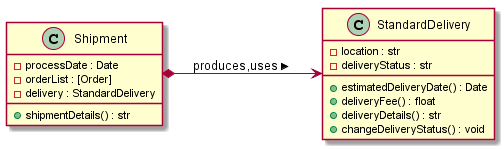
\includegraphics[keepaspectratio]{https://raw.githubusercontent.com/HowDoIGitHelp/CMSC23MDNotes/master/Markdown\%20Lecture\%20Notes\%20and\%20Lab\%20Exercises/uml/nonfactorymethodExample.png}}
\caption{online marketplace}
\end{figure}

\begin{Shaded}
\begin{Highlighting}[]
\ImportTok{from}\NormalTok{ datetime }\ImportTok{import}\NormalTok{ date,timedelta}

\KeywordTok{class}\NormalTok{ Order:}
    \KeywordTok{def} \FunctionTok{\_\_init\_\_}\NormalTok{(}\VariableTok{self}\NormalTok{,productName:}\BuiltInTok{str}\NormalTok{, productPrice:}\BuiltInTok{float}\NormalTok{):}
        \VariableTok{self}\NormalTok{.\_\_productName }\OperatorTok{=}\NormalTok{ productName}
        \VariableTok{self}\NormalTok{.\_\_productPrice }\OperatorTok{=}\NormalTok{ productPrice}
    \KeywordTok{def}\NormalTok{ orderString(}\VariableTok{self}\NormalTok{) }\OperatorTok{{-}\textgreater{}} \BuiltInTok{str}\NormalTok{:}
        \ControlFlowTok{return} \StringTok{"}\SpecialCharTok{\%s}\StringTok{ P}\SpecialCharTok{\%.2f}\StringTok{"} \OperatorTok{\%}\NormalTok{ (}\VariableTok{self}\NormalTok{.\_\_productName,}\VariableTok{self}\NormalTok{.\_\_productPrice)}
    \KeywordTok{def}\NormalTok{ price(}\VariableTok{self}\NormalTok{) }\OperatorTok{{-}\textgreater{}} \BuiltInTok{float}\NormalTok{:}
        \ControlFlowTok{return} \VariableTok{self}\NormalTok{.\_\_productPrice}

\KeywordTok{class}\NormalTok{ StandardDelivery:}
    \KeywordTok{def} \FunctionTok{\_\_init\_\_}\NormalTok{(}\VariableTok{self}\NormalTok{,location:}\BuiltInTok{str}\NormalTok{):}
        \VariableTok{self}\NormalTok{.\_\_location }\OperatorTok{=}\NormalTok{ location}
        \VariableTok{self}\NormalTok{.\_\_deliveryStatus }\OperatorTok{=} \StringTok{"Processing"}
    \KeywordTok{def}\NormalTok{ deliveryDetails(}\VariableTok{self}\NormalTok{) }\OperatorTok{{-}\textgreater{}} \BuiltInTok{str}\NormalTok{:}
\NormalTok{        r }\OperatorTok{=} \StringTok{"STANDARD DELIVERY}\CharTok{\textbackslash{}n}\StringTok{DELIVER TO:}\SpecialCharTok{\%s}\CharTok{\textbackslash{}n}\StringTok{DELIVERY STATUS: }\SpecialCharTok{\%s}\CharTok{\textbackslash{}n}\StringTok{DELIVERY FEE: P}\SpecialCharTok{\%.2f}\StringTok{"} \OperatorTok{\%}\NormalTok{ (}\VariableTok{self}\NormalTok{.\_\_location,}\VariableTok{self}\NormalTok{.\_\_deliveryStatus,}\VariableTok{self}\NormalTok{.deliveryFee())}
        \ControlFlowTok{return}\NormalTok{ r}
    \KeywordTok{def}\NormalTok{ deliveryFee(}\VariableTok{self}\NormalTok{) }\OperatorTok{{-}\textgreater{}} \BuiltInTok{float}\NormalTok{:}
        \ControlFlowTok{return} \DecValTok{500}
    \KeywordTok{def}\NormalTok{ estimatedDeliveryDate(}\VariableTok{self}\NormalTok{,processDate:date) }\OperatorTok{{-}\textgreater{}} \BuiltInTok{float}\NormalTok{:}
        \ControlFlowTok{return}\NormalTok{ processDate }\OperatorTok{+}\NormalTok{ timedelta(days }\OperatorTok{=} \DecValTok{7}\NormalTok{)}
    \KeywordTok{def}\NormalTok{ changeDeliveryStatus(}\VariableTok{self}\NormalTok{,newStatus:}\BuiltInTok{str}\NormalTok{):}
        \VariableTok{self}\NormalTok{.\_\_deliveryStatus }\OperatorTok{=}\NormalTok{ newStatus}

\KeywordTok{class}\NormalTok{ Shipment:}
    \KeywordTok{def} \FunctionTok{\_\_init\_\_}\NormalTok{(}\VariableTok{self}\NormalTok{, orderList:}\BuiltInTok{list}\NormalTok{[Order], processDate: date, location):}
        \VariableTok{self}\NormalTok{.\_orderList }\OperatorTok{=}\NormalTok{ orderList}
        \VariableTok{self}\NormalTok{.\_processDate }\OperatorTok{=}\NormalTok{ processDate}
        \VariableTok{self}\NormalTok{.\_delivery }\OperatorTok{=}\NormalTok{ StandardDelivery(location)}

    \KeywordTok{def}\NormalTok{ totalPrice(}\VariableTok{self}\NormalTok{) }\OperatorTok{{-}\textgreater{}} \BuiltInTok{str}\NormalTok{:}
\NormalTok{        t }\OperatorTok{=} \FloatTok{0.0}
        \ControlFlowTok{for}\NormalTok{ order }\KeywordTok{in} \VariableTok{self}\NormalTok{.\_orderList:}
\NormalTok{            t}\OperatorTok{+=}\NormalTok{order.price()}
        \ControlFlowTok{return}\NormalTok{ t}

    \KeywordTok{def}\NormalTok{ shipmentDetails(}\VariableTok{self}\NormalTok{) }\OperatorTok{{-}\textgreater{}} \BuiltInTok{str}\NormalTok{:}
\NormalTok{        r }\OperatorTok{=} \StringTok{"ORDERS:"} \OperatorTok{+} \BuiltInTok{str}\NormalTok{(}\VariableTok{self}\NormalTok{.\_processDate) }\OperatorTok{+} \StringTok{"}\CharTok{\textbackslash{}n}\StringTok{"}
        \ControlFlowTok{for}\NormalTok{ order }\KeywordTok{in} \VariableTok{self}\NormalTok{.\_orderList:}
\NormalTok{            r }\OperatorTok{+=}\NormalTok{ order.orderString() }\OperatorTok{+} \StringTok{"}\CharTok{\textbackslash{}n}\StringTok{"}
\NormalTok{        r }\OperatorTok{+=} \StringTok{"}\CharTok{\textbackslash{}n}\StringTok{"}
\NormalTok{        r }\OperatorTok{+=} \StringTok{"TOTAL PRICE OF ORDERS: P"}  \OperatorTok{+} \BuiltInTok{str}\NormalTok{(}\VariableTok{self}\NormalTok{.totalPrice()) }\OperatorTok{+} \StringTok{"}\CharTok{\textbackslash{}n}\StringTok{"}
\NormalTok{        r }\OperatorTok{+=} \VariableTok{self}\NormalTok{.\_delivery.deliveryDetails() }\OperatorTok{+} \StringTok{"}\CharTok{\textbackslash{}n\textbackslash{}n}\StringTok{"}
\NormalTok{        r }\OperatorTok{+=} \StringTok{"PRICE WITH DELIVERY FEE : P"} \OperatorTok{+} \BuiltInTok{str}\NormalTok{(}\VariableTok{self}\NormalTok{.totalPrice()}\OperatorTok{+}\VariableTok{self}\NormalTok{.\_delivery.deliveryFee()) }\OperatorTok{+} \StringTok{"}\CharTok{\textbackslash{}n}\StringTok{"}
\NormalTok{        r }\OperatorTok{+=} \StringTok{"ESTIMATED DELIVERY DATE: "} \OperatorTok{+} \BuiltInTok{str}\NormalTok{(}\VariableTok{self}\NormalTok{.\_delivery.estimatedDeliveryDate(}\VariableTok{self}\NormalTok{.\_processDate))}
        \ControlFlowTok{return}\NormalTok{ r}

\NormalTok{o }\OperatorTok{=}\NormalTok{ [Order(}\StringTok{"Surface Pro 7"}\NormalTok{,}\DecValTok{40000}\NormalTok{),Order(}\StringTok{"Zzzquil"}\NormalTok{,}\DecValTok{900}\NormalTok{)]}
\NormalTok{s }\OperatorTok{=}\NormalTok{ Shipment(o,date(}\DecValTok{2019}\NormalTok{,}\DecValTok{11}\NormalTok{,}\DecValTok{1}\NormalTok{),}\StringTok{"Cebu City"}\NormalTok{)}
\BuiltInTok{print}\NormalTok{(s.shipmentDetails())}
\end{Highlighting}
\end{Shaded}

This system does work. It works but it is still inelegant. As soon as
your app grows, you will incorporate new delivery options like express
delivery, or pickups or whatever. Every time you need to add a new
delivery method you will need to perform surgery in \texttt{Shipment}
since the \texttt{StandardDelivery} instance is created inside the
constructor of \texttt{Shipment}. \texttt{Shipment}'s code is too
coupled with \texttt{StandardDelivery}.

To solve this you need to implement the factory method pattern. Right
now shipment is a factory since it constructs its own instance of
\texttt{StandardDelivery}. To refactor this into elegant code, you need
to so create an abstraction called\texttt{Delivery} first to support
polymorphism. Inside \texttt{Shipment} instead of creating instances of
\texttt{Delivery}'s using a constructor, you invoke a factory method
that encapsulates the instantiation of \texttt{Delivery}. In this case
we name this method \texttt{newDelivery()}. All it does is return an
instance of \texttt{StandardDelivery} using its constructor.

\begin{figure}
\centering
\pandocbounded{\includegraphics[keepaspectratio]{https://raw.githubusercontent.com/HowDoIGitHelp/CMSC23MDNotes/master/Markdown\%20Lecture\%20Notes\%20and\%20Lab\%20Exercises/uml/factorymethodExample.png}}
\caption{online marketplace}
\end{figure}

In this new architecture, whenever there are new delivery methods a
shipment could have, all you have to do is to create a realization of
that delivery method. In this case the new delivery method is
\texttt{ExpressDelivery} which delivers the next day but is twice as
expensive. And instead of changing \texttt{Shipment} (violates
Open/Closed Principle), you make an extension to \texttt{Shipment}. This
extension is the specialization to shipment called
\texttt{ExpressShipment} (a shipment that uses express delivery). In
this specialization, you only need to override the factory method
delivery, so that every instance of delivery construction creates
\texttt{ExpressDelivery}. The difference between
\texttt{ExpressDelivery} and \texttt{Delivery} is that
\texttt{ExpressDelivery} has a delivery fee of 1000 and the estimated
delivery date is one day after the processing date.

\textbf{Complete the system using the factory method pattern.}

\section{Assessment
Criteria}\label{lab-exercise-8-shipment.md__assessment-criteria}

\begin{itemize}
\tightlist
\item
  Completeness of the pattern - 40
\item
  Elegance of method and attribute naming - 10
\end{itemize}
